\documentclass[a6paper,fontsize=10pt,twoside,open=right]{scrbook}
\usepackage[a6paper,top=1cm,bottom=1.9cm,left=1cm,right=1cm,footskip=1cm,headsep=0.2cm]{geometry}% ,showframe
\usepackage[swedish]{babel}
\usepackage[utf8]{inputenc}
\usepackage[T1]{fontenc}
\usepackage{graphicx}
\usepackage{tocloft}
\usepackage{metalogo}
\usepackage{titletoc}
\usepackage{titlesec}
\usepackage{eso-pic}
\usepackage{scrpage2}
\usepackage{anyfontsize}
\usepackage{microtype}
\usepackage{array}
\usepackage{marvosym}
\usepackage{mdframed}
\usepackage{textcomp}
\usepackage{amssymb}
\usepackage{enumitem}
\usepackage{letltxmacro}
\usepackage[columns=1]{idxlayout}
\usepackage[bitstream-charter]{mathdesign}
\usepackage{hyphenat}
\usepackage{setspace}
\usepackage{makeidx}
\usepackage{overpic,textpos,hyperref}
\usepackage{alltt}
\usepackage{indentfirst}
\renewcommand{\ttdefault}{txtt}
\tracinggroups=1

\newgeometry{top=1cm,bottom=1cm,left=1cm,right=1cm,footskip=0pt,headsep=0.2cm,footskip=0.3cm}

%\setlength{\emergencystretch}{2em}

\LetLtxMacro\origttfamily\ttfamily
\DeclareRobustCommand*{\ttfamily}{%
  \origttfamily
  \hyphenchar\font=`\-\relax
  \fontdimen3\font=.25em\relax
  \fontdimen4\font=.167em\relax
  \fontdimen7\font=.167em\relax
}

%\usepackage[ebgaramond-maths]{mathdesign}

%% Gömma varningar om underfull \hbox
%% \hbadness=10001

%% \tolerance=1
%% \emergencystretch=\maxdimen
%% \hyphenpenalty
%% \exhyphenpenalty

\renewcommand{\baselinestretch}{0.98} 

\makeindex

\let\oldemptyset\emptyset
\let\emptyset\varnothing

%% eso-pic for background on chapter pages %%
%\newcommand\BackgroundPic{\includegraphics[width=\paperwidth,height=\paperheight,keepaspectratio]{elements/chapter2.pdf}}

%% scrpage2 pagestyling %%
\pagestyle{scrheadings}
\clearscrheadfoot

%% change empty page produced by \cleardoublepage into scrheading style %%
\makeatletter
\let\ps@empty\ps@scrheadings
\makeatother

\newcommand{\rpt}{
        \raisebox{.2ex}{:}
        \hspace*{-0.5ex}\raisebox{-.4ex}{\rule{.1ex}{2.3ex}\,\rule{.2ex}{2.3ex}}}

\newcommand{\revrpt}{
        \raisebox{-.4ex}{\rule{.2ex}{2.3ex}\,\rule{.1ex}{2.3ex}}
        \hspace*{-0.5ex}\raisebox{.2ex}{: }}

%% chapter and section styling %%
\titleformat{\chapter}{}{}{0pt}{\vspace*{20pt}\centering\fontsize{30}{40}\rmfamily\textbf}
\titleformat{\section}{}{}{0pt}{\fontsize{13}{15}\rmfamily\textbf}
\titlespacing*{\section}{0pt}{0pt}{0pt}
\titlespacing*{\chapter}{0pt}{0pt}{40pt}
\titlecontents{chapter}[0em]{\addvspace{3pt}}{\contentslabel{}}{}{\titlerule*[0.3pc]{.}\hspace*{-4pt}\contentspage}

\makeatletter
\def\emptypage@emptypage{%
  \hbox{}%
  \blankpage%
  \newpage%    
}%
\def\cleardoublepage{%
  \ohead{}\null
  \if@twoside%
  \ifodd\c@page%
  % do nothing
  \else%
  \emptypage@emptypage%
  \fi%
  \fi%
}%
\makeatother

%% Command for chapter page, will remove foot and head %%
\newcommand{\chapterpage}[2]{
  \newpage
  \null
  \cleardoublepage
  %\AddToShipoutPicture*{\BackgroundPic}
  \chapter[#1]{#2}
  \renewcommand{\leftmark}{#1}
  \newpage
  \ohead{\textnormal{\textsc{\scriptsize\leftmark}}}
  \ofoot[\pagemark]{\textsc{\scriptsize\pagemark}}
  %\cfoot{\centering\includegraphics[keepaspectratio]{elements/footelement2.pdf}}
}
\newcommand{\chapterpageimage}[3]{
  \newpage
  \null
  \cleardoublepage
  \chapter[#1]{#2}
  \vspace*{-35pt}
  \begin{center}
    \includegraphics[keepaspectratio,height=0.65\textheight]{#3}
  \end{center}
  \renewcommand{\leftmark}{#1}
  \newpage
  \ohead{\textnormal{\textsc{\scriptsize\leftmark}}}
  \ofoot[\pagemark]{\textsc{\scriptsize\pagemark}}
  %\cfoot{\centering\includegraphics[keepaspectratio]{elements/footelement2.pdf}}
}
\newcommand{\hiddenchapterpage}[1]{
  \newpage
  \null
  \cleardoublepage
  %\AddToShipoutPicture*{\BackgroundPic}
  \chapter*{#1}
  \renewcommand{\leftmark}{#1}
  \newpage
  \ohead{\textnormal{\textsc{\scriptsize\leftmark}}}
  \ofoot[\pagemark]{\textsc{\scriptsize\pagemark}}
  %\cfoot{\centering\includegraphics[keepaspectratio]{elements/footelement2.pdf}}
}
\makeatletter
\renewcommand\chapter{\if@openright\cleardoublepage\else\clearpage\fi
  \thispagestyle{empty}
  \global\@topnum\z@
  \@afterindentfalse
  \ofoot[\pagemark]{\textsc{\scriptsize\pagemark}}
  \cfoot{}
  \ohead{}
  \secdef\@chapter\@schapter}
\makeatother

\newcommand{\specialcell}[2][c]{
  \begin{tabular}[#1]{@{}l@{}}#2\end{tabular}} 

%% Command for songs %%
\newcommand{\visa}[1]{%
  \index{\uppercase{#1}}%
  \section{\uppercase{#1}}%
}
\newcommand{\fvisa}[2]{%
  \index{\uppercase{#1}}\index{#2}%
  \section{\uppercase{#1}}%
}
\newcommand{\kvisa}[2]{%
  \index{\uppercase{#1}}
  \section{\uppercase{#2}}%
}
\newcommand{\svisa}[3]{%
  \index{\uppercase{#1}}\index{#2}%
  \section{\uppercase{#3}}%
}
\newcommand{\tvisa}[1]{%
  \index{Ã#1@\uppercase{#1}}
  \section{\uppercase{#1}}%
}

%% TOC %%
\setcounter{tocdepth}{0}
\tocloftpagestyle{scrheadings}

%% MISC %%
\pagenumbering{arabic}
\renewcommand{\chaptername}{}
\renewcommand{\thechapter}{}
\renewcommand{\thesection}{}

\makeatletter
\renewenvironment{theindex}
                 {{\noindent\rmfamily{\fontsize{13}{15}\textbf{TITEL och FÖRSTARADEN REGISTER}}\vspace*{10pt}\par\textbf{\normalsize \#}\par}
                   \@mkboth{\MakeUppercase\indexname}
                           {\MakeUppercase\indexname}
                           \let\item\@idxitem}
                 {}
\makeatother
\newmdenv[
  topline=false,
  bottomline=false,
  rightline=false,
  linewidth=1pt,
  skipabove=5pt,
  skipbelow=3pt,
  innertopmargin=0pt,
  innerbottommargin=0pt
]{leftborder}
\makeatletter

\newcommand*\cleartoleftpage{%
  \clearpage
  \ifodd\value{page}\hbox{}\newpage\fi
}

\newcommand\textline[4][t]{%
  \vspace*{-5pt}\hfill\par\smallskip\noindent\parbox[#1]{.266\textwidth}{\raggedright\strut#2}%
  \parbox[#1]{.266\textwidth}{\centering\strut#3}%
  \parbox[#1]{.266\textwidth}{\raggedleft\strut#4}\hfill\par\smallskip%
}

\begin{document}
\vspace*{6.5cm}
\hspace*{0.9cm}

\includegraphics[keepaspectratio,width=7cm]{elements/logo.pdf}
\clearpage
\noindent Denna fantasmagoriska manual tillhör:
\ohead{\textnormal{\textsc{\scriptsize\leftmark}}}
\ofoot[\pagemark]{\textsc{\scriptsize\pagemark}}
\clearpage
\index{ÃDatavetare är skapande människor@\uppercase{Datavetare är skapande människor}}
{\small\begin{verbatim}
Datavetare är skapande människor

Datavetare skapar. De skapar nya program som
världen aldrig sett tidigare, för att låta
datorer göra saker som de aldrig gjort tidigare.
De forskar fram nya kunskaper och öppnar nya
fält för framtidens forskning. Datavetare skapar
de verktyg som gör det möjligt att lösa nya problem.
Nya programmeringsspråk, nya beräkningsverktyg,
bättre kompilatorer, bättre databaser, nya
operativsystem, bättre utvecklingsverktyg,
distribuerade system... Listan kan göras hur lång
som helst.
  
Datavetenskapens handfasta mål är att förbättra
den programvara som vi kör på våra datorer. Vad
som krävs är att programmen gör vad de skall
(korrekthet), att de inte gör fel om något
oförutsett inträffar (pålitlighet), och att de
arbetar effektivt (effektivitet). Dessutom skall
programmen utvecklas på ett effektivt sett.
\end{verbatim}}
\vspace{10pt}
\noindent{\footnotesize\textit{Ur ``Vad är en datavetare
egentligen''\\ BlurGel nr 0, 1995}}
\clearpage
\setlength{\parindent}{15pt}
%\newgeometry{top=1cm,bottom=1.2cm,left=1cm,right=1cm,footskip=0pt,headsep=0.2cm}
\null
\vfill
    {\noindent\small\centering
      Redaktör: Janne\\
      Grafisk formgivare: Per Bergqwist\\
      Illustratör: Paulina Hermansson\\
      Logotyp: Jens Bohlin\\
      Producerad med \LaTeX\\
      v1.0: 1994-11-21 (1000 exemplar)\\
      v1.1: 1996-01-02 (1000 exemplar)\\
      v2.001: 2001-11-15 (1000 exemplar)\\
      vJub: 2011-11-11 (300 exemplar)\\
      v3.0: 2015-??-?? (1200 exemplar)\\
      Tryckeri: Boktryckarna\par
    }
%\restoregeometry
\cleardoublepage
%\cfoot{\centering\includegraphics[keepaspectratio]{elements/footelement2.pdf}}
\section{FÖRORD}
\vspace{10pt}
Den manual du nu håller i din hand är en del av ett stycke
historia. Den första manualen trycktes nämligen år 1994 och totalt har
det tryckts fyra upplagor, inklusive Jubileumsmanualen som trycktes
till trettioårsjubileet för datavetarutbildningen i Uppsala.

Historiskt sett har manualen producerats gemensamt av datavetarna i
Uppsala, Linköping och Umeå. Alldeles nyligen upphörde dock Linköping
med sin datavetarutbildning och Umeå verkar ha haft problem med sin
mailserver, då vi inte fick några svar därifrån.

Under 2014 och 2015 samlades en ädel grupp upsaliensisiska datavetare
under ouppräkneligt många timmar av möten för att fastställa
innehållet av den nya manualen. Det resulterade i återupplivandet av
många sånger ifrån gamla upplagor men ännu fler nya sånger som aldrig
funnits i manualen tidigare lades in, bland annat skapades ett helt
nytt kapitel vid namn ``Interwebz''.\par
\vspace{10pt}
\noindent Uppsala, 2 Juli 2015\\
Manualgruppen\\
\begin{center}
  \parbox{0.47\textwidth}{
    \vspace*{-7pt}
    Per ``normano'' Bergqwist\\
    {@}Jens Rosén\\
    Lukas ``spydon'' Klingsbo\\
    Aleksander ``Tan'' Lundqvist\\
    Patrik ``Klutt'' Broman\\
    Jakob ``KP'' Mattsson\\
    Oskar ``osaka'' Ahlberg\\
    Johan ``Johan'' Lundgren}
\end{center}
\null
\vspace*{-10pt}
\newpage
Ett stort tack till alla de som donerat till skapandet av denna manual
och ett extra stort tack till Pu som skapat alla illustrationer till
kapitlena.\par
\vspace{10pt}
\begin{tabular}{@{}p{0.5\textwidth}p{0.5\textwidth}@{}}
  Christian Axelsson & Andrée Bylund\\
  Niklas Carlsson & Jakob Engblom\\
  Martin Frost & Paulina Hermansson\\
  Joakim Hägglund & Måns af Klercker\\
  Catarina Malmberg & Niklas Malmberg\\
  Pär Mattsson & Hans Molin\\
  Samuel Strand & Markus Säfström\\
  Niclas Stensbäck & Erika Wahlberg\\
  Jesper Wilhelmsson & Ingemar {\fontsize{9pt}{0pt}\selectfont Å}berg
\end{tabular}\par
\vfill
\begin{center}
  \noindent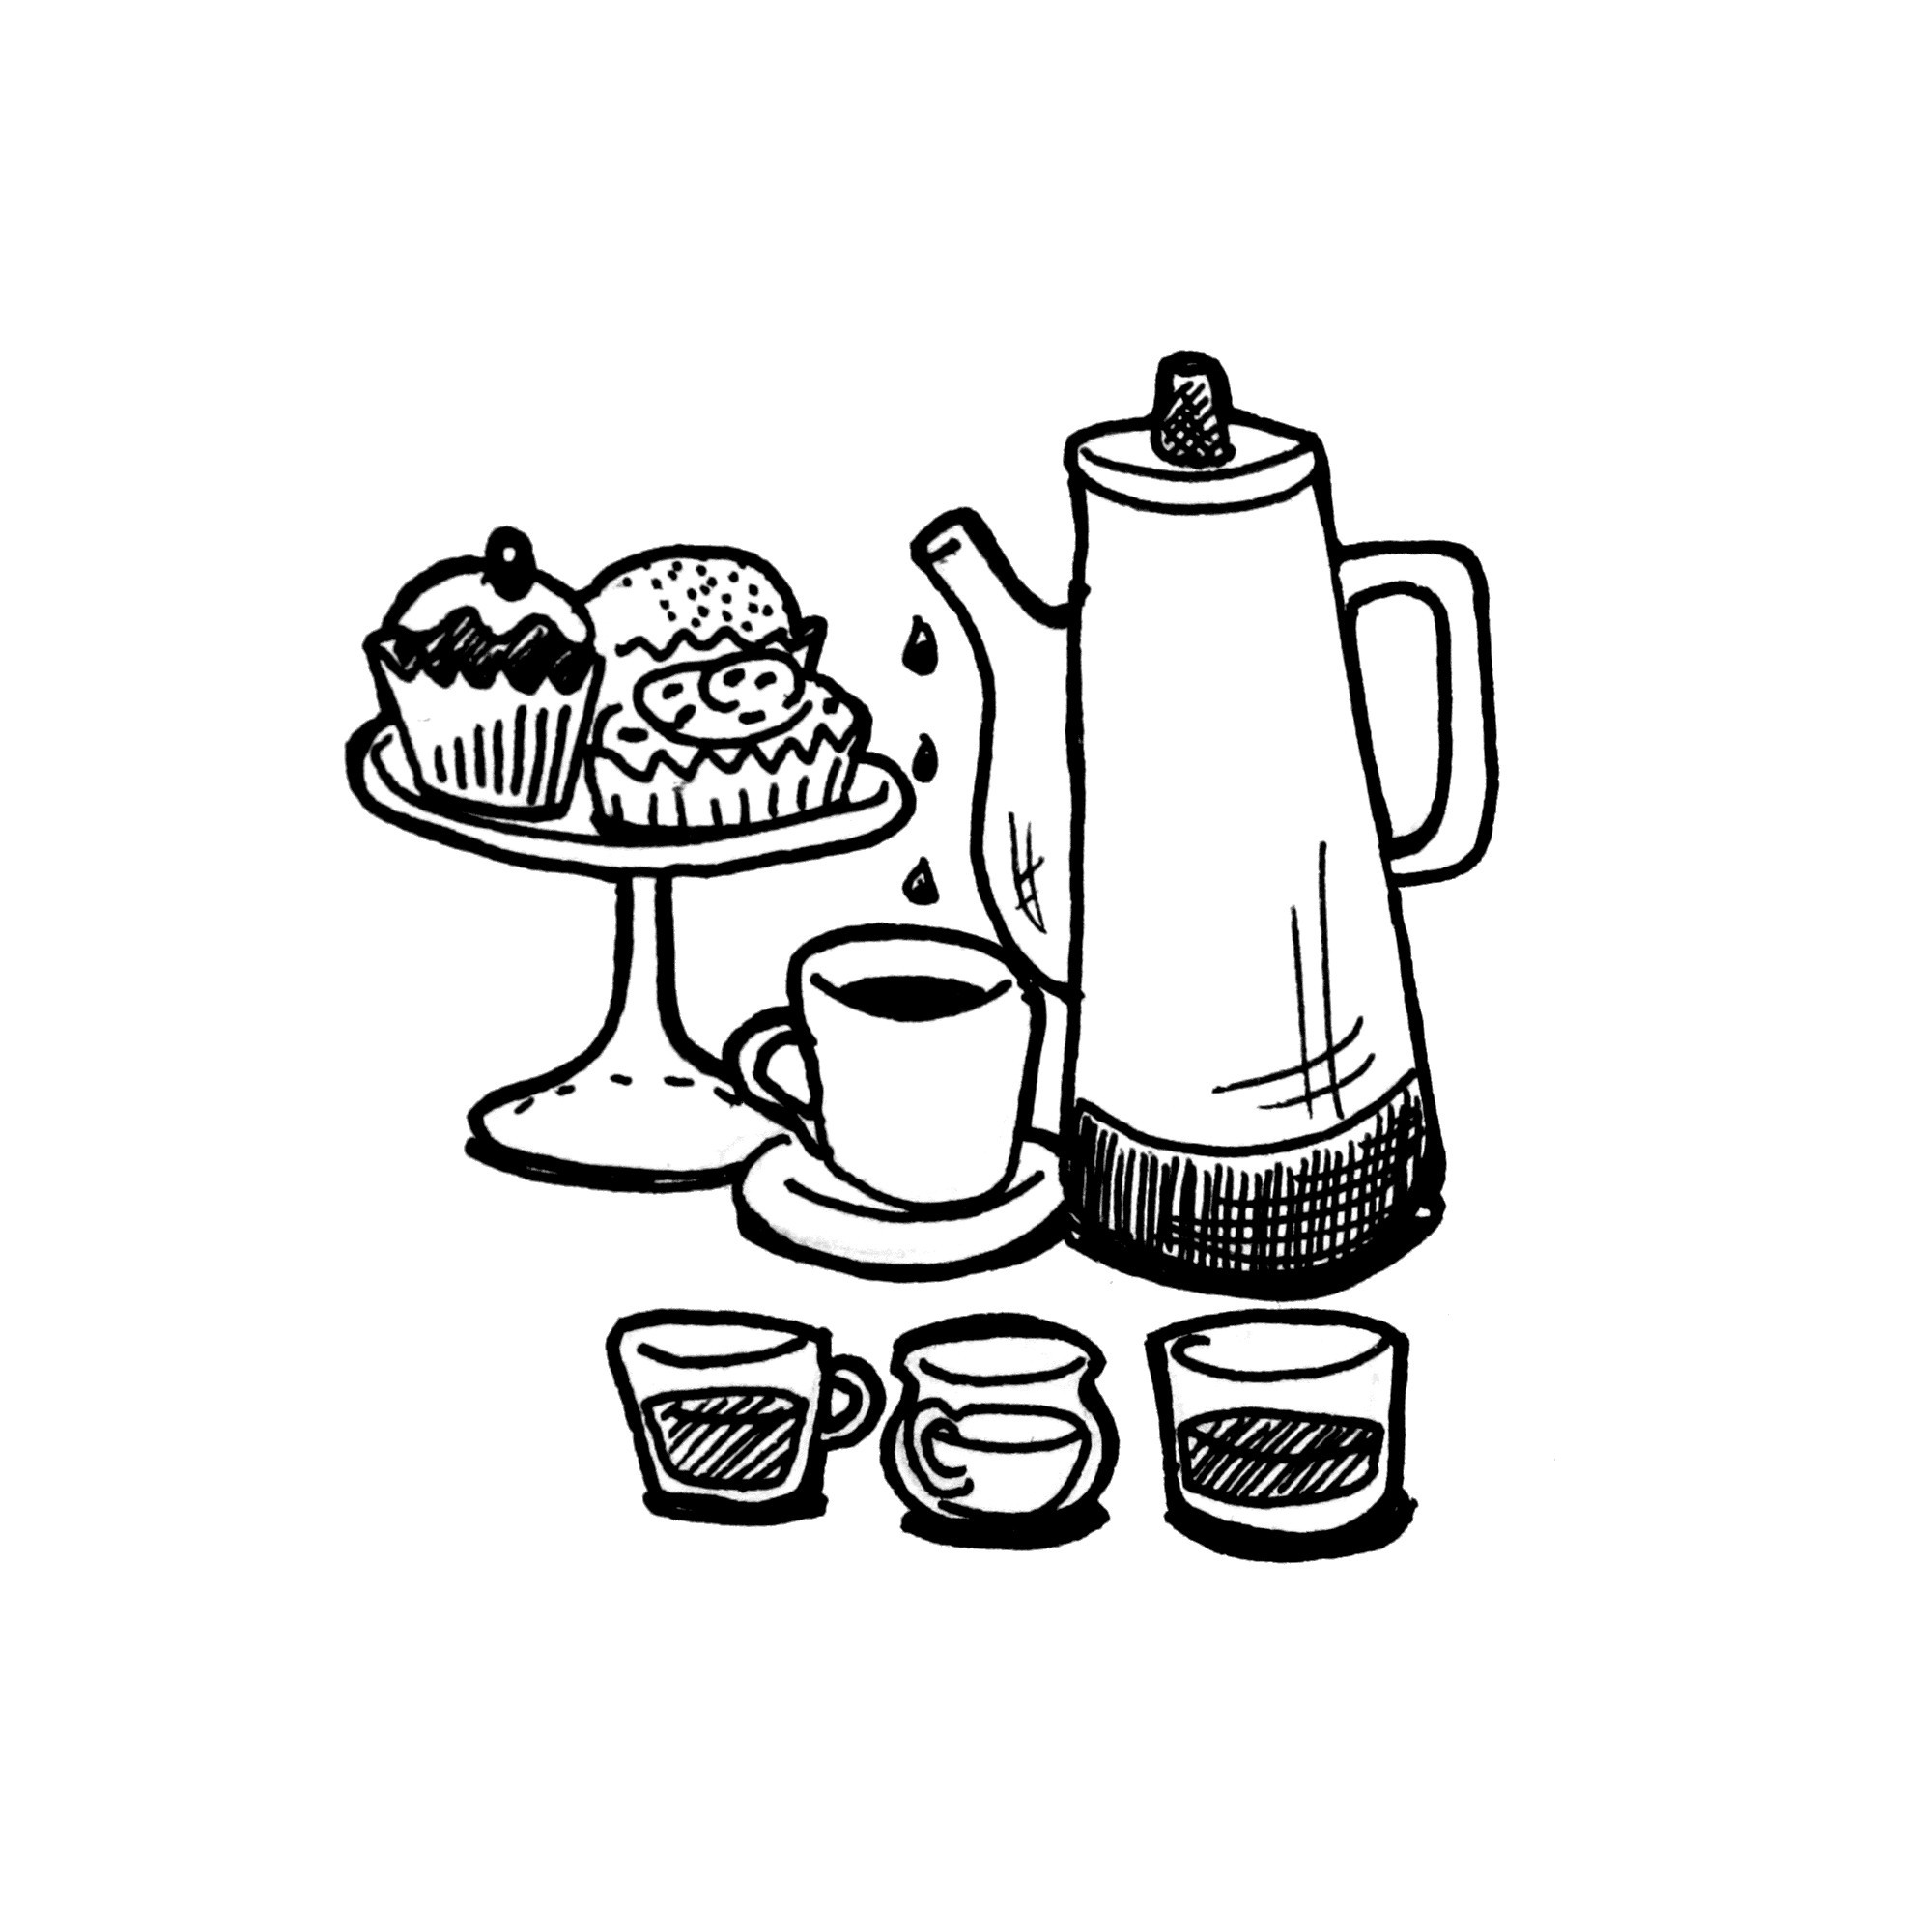
\includegraphics[keepaspectratio,width=0.6\textwidth]{elements/punsch1.jpg}\par
  \noindent \footnotesize{Den nedröstade kakbilden}
\end{center}
\vfill
\null
\newpage
Vi vill även tacka alla som hjälpte till med skapandet av de äldre
manualerna, utan ert arbete skulle denna bok inte vara här idag.\par
\vspace{10pt}
\begin{tabular}{@{}p{0.5\textwidth}p{0.5\textwidth}@{}}
  Anders Jackson & Anders Jansson\\
  Anders Ramsell & Anders Wilhelm\\
  Andreas Gref & Andreas Hed\\
  Bertil Spolander & Björn Bergman\\
  Björn Knutsson & Björn Knutsson\\
  Björn Torkelsson & Calle Englund\\
  Daniel Gref & Daniel Holmgren\\
  Egil Salomonsson & Emilio Nyaray\\
  Erik Åhlin & Erika Elmquist\\
  Göran Svensson & Hans Molin\\
  Henrik Eriksson & Håkan Lindholm\\
  Ingela Anderton & Ingela Ljungkvist\\
  Jakob Engblom & Jan-Olof Flink\\
  Jens Bohlin & Jens Rosén\\
  Jesper Wilhelmsson & Joakim Lindqvist\\
  Joakim Thörnkvist & Johan Lundgren\\
  Jonas Högström & Kristiina Ausmees\\
  Lars Hägglund & Lars-Arne Mattson\\
  Lukas Klingsbo & Martin Davidson\\
  Mats Hägglund & Mattias Hallberg\\
  Micke Liljeblad & Måns Engmem\\
  Måns af Klercker & NeNNe\\
  Niclas Stensbäck & Olof Appelblad\\
  Olof Dahlberg & Pär Mattsson\\
  Sandra Nyström & Sara Ingmar
\end{tabular}
\newpage
\index{ÃTRAVERSERING@\uppercase{TRAVERSERING}}
\section{TRAVERSERING}\vspace{10pt}
Genom hela denna bok gäller följande
traverseringsregler. I sånger där en försångare eller dylikt skall
sjunga ensam används fet text. Ifall något speciellt såsom en handling
inträffar vid ett ord, så används (kursiv), där ordet för handling
eller beteende står inom ( ). En sådan handling gäller oftast maximalt
raden ut. Ifall en längre förklaring behövs kursiveras
texten. Beskrivningen finns sedan efter sångens slut. I denna
beskrivning kan mycket annat matnyttigt finnas, läs den
gärna.

I en del sånger sjunges inte hela sången tillsammans,
istället är delar av sången menat för ena gruppen och vice versa. I
dessa sånger används {\Large\Male} för manligt kön och {\Large\Female}
för kvinnligt kön, men du får givetvis sjunga vilken del du vill.

\begin{leftborder}
  \hspace{15pt}Då det ibland kan förekomma lokala variantioner på vissa sånger, så
  används en  vertikal linje i högra kanten för att markera att detta
  är olika alternativ. Ibland betyder linjen att det är raderna som är
  alternativen, och ibland betyder linjen att det är olika
  versalternativ. Men den kloke läsaren förstår säkert när vad är vad.
\end{leftborder}

För att göra allt ännu svårare så skall man oftast sjunga med stark
stämma där VERSALER används, men observera att man inte alltid skall
göra detta. Vem har sagt att det skall vara lätt?
\newpage
%% begin toc on odd page and style the title %%
\cleardoublepage
\renewcommand{\contentsname}{\vspace{-2.17cm}\rmfamily{\fontsize{13}{15}\textbf{INNEHÅLL}}\vspace{45pt}}
\tableofcontents\par
\begin{center}
  \vspace*{-300pt}
  \noindent
\includegraphics[keepaspectratio,width=0.8\textwidth]{elements/groda.jpg}
\end{center}
%% Remove the toc title from heading %%
\renewcommand{\leftmark}{}

\setlength{\parindent}{0pt}
\raggedbottom
\chapterpageimage{Av tradition}{Av tradition}{elements/avtradition.jpg}
\null
\vfill
\hfill\begin{minipage}[c]{6.7cm}
\textit{Vad bjuder oss uppriktigt Afrika?\\
Vad visa kan Amerika?\\
Vad Asien? Vad allt Europa?\\
Jag trotsar öppet alltihopa.\\
Men Skandinavien - det är alladar!\\
Blott Sverige svenska krusbär har.}\par
\vspace{10pt}
\textit{Carl Love Almquist}
\end{minipage}\hfill
\vfill
\null
\newpage
\visa{DU GAMLA, DU FRIA}
Du gamla, Du fria, Du fjällhöga nord\\
Du tysta, Du glädjerika sköna!\\
Jag hälsar Dig, vänaste land uppå jord,\\
||: Din sol, Din himmel, Dina ängder gröna. :||\\
\\
Du tronar på minnen från fornstora dar,\\
då ärat Ditt namn flög över jorden.\\
Jag vet att Du är och Du blir vad du var.\\
||: Ja, jag vill leva jag vill dö i Norden. :||\\
\\
Jag städs vill dig tjäna mitt älskade land,\\
din trohet till döden vill jag svära.\\
Din rätt, skall jag värna, med håg och med hand,\\
||: din fana, högt den bragderika bära. :||\\
\\
Med Gud skall jag kämpa, för hem och för härd,\\
för Sverige, den kära fosterjorden.\\
Jag byter Dig ej, mot allt i en värld\\
||: Nej, jag vill leva jag vill dö i Norden. :||\\
\\
{\footnotesize\textit{Text: Richard Dybeck, 1844\\
\\
Sveriges nationalsång av tradition sedan 1866.\\
De två sista verserna sjungs sällan.}}
\clearpage

\newpage
\fvisa{SVERIGES FLAGGA}{Flamma stolt mot dunkla skyar}
\vspace{10pt}
Flamma stolt mot dunkla skyar\\
lik en glimt av sommarens sol!\\
Över Sveriges skogar, berg och byar,\\
över vatten och viol!\\
Du som sjunger, när Du bredes\\
som vår gamla lyckas tolk.\\
Solen lyser! Solen lyser!\\
Ingen vredes åska slog vårt tappra folk!\par
\vspace{10pt}
Flamma högt vårt kärlekstecken!\\
Värm oss, när det blåser kallt!\\
Stråla ut de blåa vecken\\
kärlek mera stark än allt!\\
Sveriges flagga! Sveriges ära!\\
Fornklenod och framtidstolk!\\
Gud är med oss! Gud är med oss!\\
Han skall bära stark vårt fria svenska folk\par
\vspace{10pt}
{\footnotesize\textit{Text: K.G. Ossiannilsson\\
Musik: Hugo Alfvén}}

\newpage
\fvisa{NORRLANDSSÅNGEN}{Hör du, säg hör du vår norrländska låt}
\vspace{10pt}
Hör du, säg hör du vår norrländska låt\\
över vidden klinga, manande och bringa\\
hälsning till landet där mångmila stråt\\
banande når den bygden som är vår?\\
\\
Älvarnas silver i mörknande skog.\\
Bergsmassiv som gråna och sin märg oss låna.\\
Skälvande mylla bak vändande plog.\\
Havets vida famn med skötar, grund och hamn.\\
\\
Norrland är vårt rike, landet utan like.\\
Storvulet vilt eller leende och milt.\\
I mitt sinne leka jublande veka\\
sånger ibland om min hembygds fagra land.\\
\\
Lyft då ditt huvud och räta din rygg!\\
Stoltare än andra kan du vägen vandra.\\
Norrlänning är du och ärlig och trygg.\\
Sjung din vandringslåt på norrländsk färdestråt!\\
\\
{\footnotesize\textit{Text: Torsten Sundelin\\
Musik: Hjalmar Palmgren}}

\newpage
\fvisa{JÄMTLANDSSÅNGEN}{Så tåga vi tillsammans bort}
\vspace{10pt}
Så tåga vi tillsammans bort\\
mellan Jämtlands gröna ängar\\
bort mellan nyland som prunka\\
fulla av bröllopsblomsters prakt.\\
Så skådom nu med gamman hän\\
emot berg i blåa fjärran hän,\\
över sjöar, strömmar, skogar\\
jämt kring bygder på vakt.\par
\vspace{10pt}
\revrpt Fagert är landet\\
som blev vår lott och arvedel.\\
Så firom dess fägring nu\\
med sång och stråkars spel.\\
Så tändom ånyo det hopp\\
som våra fäder närt.\\
För slit och mödor\\
av fröjd och sol\\
ett mått oss beskärt\rpt\par
\vspace{10pt}
{\footnotesize\textit{Text \& Musik: Wilhelm Peterson-Berger}}

\newpage
\fvisa{VÄRMLANDSVISAN}{Ack värmeland, du sköna}
\vspace{10pt}
Ack, Värmeland, du sköna, du härliga land!\\
Du krona för Svea rikes länder!\\
Ja, om jag komme mitt i det förlovade land,\\
till Värmland jag ändå återvänder.\\
Ja, där vill jag leva, ja, där vill jag dö.\\
Om en gång ifrån Värmland jag tager mig en mö,\\
så vet jag att aldrig jag mig ångrar.\par
\vspace{10pt}
I Värmeland är lustigt att leva och bo;\\
det landet jag prisar så gärna.\\
Där klappar det hjärtan med heder och tro\\
så fasta som bergenas kärna.\\
Och var och en svensk uti Svea rikes land,\\
som kommer att gästa vid Klarälvens strand,\\
han finner blott bröder och systrar.\par
\vspace{10pt}
I Värmeland - ja där vill jag bygga och bo,\\
med enklaste lycka förnöjder.\\
Dess dalar och skog ge mig tystnadens ro,\\
och luften är frisk på dess höjder.\\
Och forsarna sjunga sin ljuvliga sång -\\
vid den vill jag somna så stilla en gång\\
och vila i värmländska jorden.\par
\vspace{10pt}
{\footnotesize\textit{Text: A. Fryxell}}

\newpage
\visa{UNDER SVEA BANÈR}
\vspace{10pt}
Under Svea Banér Himlen seger oss ger;\\
Då för Konung och Land Äran lyfter sin hand.\\
Ännu Svearnes mod sif bereder en Stod\\
Utaf Lagrarne höjd, fast besglad mes blod.\\
Himlen gifve oss frid!\\
Men om den icke vinne utan vapen och strid,\\
Blifve Segern då vår, ögat offre sin tår\\
Den som faller, ock rätta till vår tacksamhet får.\\
\\
{\footnotesize\textit{Text: Samuel Ödmann\\
Musik: Johann Christian Friedrich Haeffner\\
\\
Anses vara den första upsaloensiska studentsången. Musiken hade
skrivits tidigare som soldatkör till Hæffners opera “Renaud” (\oldstylenums{1801}).\\
\\
Framfördes första gången, mitt under kriget mot Ryssland,
den \oldstylenums24} oktober \oldstylenums{1808}. Detta skedde vid en
uppvakting för fältmarskalkten Klingspor på genomresa från Finland
till Stockholm som gästade landshövding Uppsala slott.  Uppsalas
studenter marscherade då upp till slottet. Sångerna gick i täten och
sjöng denna sång.}}

\newpage
\fvisa{STUDENTSÅNGEN}{Sjungom studentens lyckliga dag}
\vspace{10pt}
Sjungom studentens lyckliga dag\\
låtom oss fröjdas i ungdomens vår!\\
Än klappar hjärtat med friska slag\\
och den ljusnande framtid är vår.\\
Inga stormar än i våra sinnen bo\\
hoppet är vår vän, och vi dess löften tro,\\
när vi knyta förbund i den lund,\\
där de härliga lagrarna gro,\\
där de härliga lagrarna gro,\\
Hurra!\par
\vspace{10pt}
Svea vår moder hugstor och skön,\\
manar till bragd som i fornstora dar,\\
vinkar med segerns och ärans lön,\\
med den skörd utan strid man ej tar.\\
Aldrig slockna då känslans rena brand,\\
aldrig brista må trohets helga band,\\
så i gyllene frid som i strid.\\
Liv och blod för vårt fädernesland!\\
Liv och blod för vårt fädernesland!\\
Hurra!\par
\vspace{10pt}
{\footnotesize\textit{Text: Herman Sätherberg, 1851}}\\
{\footnotesize\textit{Musik: Prins Gustaf}}

\newpage
\fvisa{KUNGSSÅNGEN}{Ur svenska hjärtans djup en gång}
\vspace{10pt}
Ur svenska hjärtans djup en gång\\
en samfälld och en enkel sång,\\
som går till kungen fram!\\
Var honom trofast och hans ätt,\\
gör kronan på hans hjässa lätt,\\
och all din tro till honom sätt,\\
du folk av frejdad stam!\par
\vspace{10pt}
O konung, folkets majestät\\
är även ditt: beskärma det\\
och värna det från fall!\\
Stå oss all världens härar mot,\\
vi blinka ej för deras hot:\\
vi lägga dem inför din fot -\\
en kunglig fotapall.\par
\vspace{10pt}
Men stundar ock vårt fall en dag,\\
från dina skuldror purpurn tag,\\
lyft av dig kronans tvång\\
och drag de kära färger på,\\
det gamla gula och det blå,\\
och med ett svärd i handen gå\\
till kamp och undergång!\par
\vspace{10pt}
Och grip vår sista fana du\\
och dristeliga för ännu\\
i döden dina män!\\
Ditt trogna folk med hjältemod\\
skall sömma av sitt bästa blod\\
en kunglig purpur varm och god,\\
och svepa dig i den.\par
\vspace{10pt}
Du himlens Herre, med oss var,\\
som förr du med oss varit har,\\
och liva på vår strand\\
det gamla lynnets art igen\\
hos sveakungen och hans män.\\
Och låt din ande vila än\\
utöver nordanland!
\par
\vspace{10pt}
{\footnotesize\textit{Text: C. V. A. Strandberg\\
Musik: Otto Lindblad}}\par
\vspace{10pt}
{\footnotesize\textit{Första och sista versen är de som brukar sjungas.}}

\newpage
\visa{DEN BLOMSTERTID NU KOMMER}
\vspace{10pt}
Den blomstertid nu kommer\\
med lust och fägring stor.\\
Du nalkas, ljuva sommar,\\
då gräs och gröda gror.\\
Med blid och livlig värma\\
till allt som varit dött,\\
sig solens strålar närma,\\
och allt blir återfött.
\vspace{10pt}
{\footnotesize\textit{Text: Israel Kolmodin \and Johan Olof Wallin}}


\vspace{15pt}
\visa{Här är gudagott att vara}
\vspace{10pt}
Här är gudagott att vara.\\
O, vad livet dock är skönt!\\
Hör, vad fröjd från fåglars skara.\\
Se, vad gräset lyser grönt!\\
Humlan surrar,\\
fjäriln prålar,\\
lärkan slår i skyn sin drill.\\
Och ur nektarfyllda skålar\\
dricka oss små blommor till.\\
\\
  {\footnotesize\textit{Text & Musik: Gunnar Wennerberg\\
      \\
      Examenssexan på Eklundshof}}

\newpage
\null
\vfill
\begin{center}
  \noindent
\includegraphics[keepaspectratio,width=0.6\textwidth]{elements/fulbild.pdf}
\end{center}
\vfill
\null
\chapterpageimage{Datavetarvisor}{Datavetarvisor}{elements/datavetar.jpg}
\newpage
\thispagestyle{empty}
\null
\vfill
{\noindent{\textit{\centering Fader Dator, som är i Salen,\\ helgad
    vare Din skärm,\\ tillkomme Ditt tangentbord,\\ ske Din vilja,
    så som i minnet,\\ så ock på nätet.\\ Vår dagliga utskrift giv
    oss idag\\ och förlåt oss våra misstag\\ trots att vi ej
    förlåta\\ dem som skyldiga äro.\\ Låt oss icke behöva
    vänta\\ och fräls oss ifrån dumpar.\\ Ty Salen är din\\ och
    Makten hos Handledaren\\ i Evighet.\\ UNIX.\\}}}
\vfill
\null
\newpage
\fvisa{DATAVETARNAS HÄRJARVISA}{Nu ska vi kompilera}
      {\footnotesize\textit{Melodi: Gärdebylåten}}\\
\\
Nu ska vi kompilera,\\
supa och penetrera\\
söka rekusioner ända in\\
till fixpunktssemantik.\\
Av induktion och basfall\\
blir man med lätthet asknall.\\
Hashtabeller parsas rekursivt\\
ifrån hår till häl\\
\\
{\footnotesize\textit{Text: Pär Mattsson och Magnus Ingelbo från DVL Uppsala.}}

\vspace{15pt}
\fvisa{JUBILEUMSVISA (MADHOUSE)}{En datavetare, han bor vid FooBar}\par
{\footnotesize\textit{Melodi: En sockerbagare}}\par
\vspace{10pt}
{En datavetare, han bor vid FooBar\\
sitter och kodar, vill aldrig blir klar\\
har overallen, han har långt hår.\\
har redan suttit i många år\\
Och denna dagen den skall nu firas\\
hopp in i duschen, sig själv omsvidas\\
dags att klippa sitt långa hår\\
tänk att det redan gått tretti år\par
\vspace{10pt}
{\footnotesize\textit{Text: Erika Elmquist, Kristiina Ausmees och Jens
Rosén från DV Uppsala}}\par
{\footnotesize\textit{Skriven inför DV
Uppsalas Jubileumsgasque (30 år jubiléet)}}\\
{\footnotesize\textit{Sjungs med fördel med
amerikansk brytning}}

\newpage
\svisa{THE BASIC SONG@\texttt{THE BASIC SONG}}{10 LET oss nu fatta i våra glas@\texttt{10 LET oss nu fatta i våra glas}}{\texttt{THE BASIC SONG}}
{\footnotesize\textit{Melodi: Mors lilla Olle}}\\
\\
\texttt{10 LET oss nu fatta i våra glas}\\
\texttt{20 INPUT en klunk utav det som där has}\\
\texttt{30 IF du fått nog THEN till 50 min vän}\\
\texttt{40 ELSE GOTO-baka till 10 igen}\\
\texttt{50 END}\\
\\
{\footnotesize\textit{Inledande radnummer sjungs ej.\\ I övrigt följs
    kommandon, ex. drick vid ``\texttt{INPUT en klunk}...''}}

\vspace{15pt}
\svisa{GE MIG MERA"!}{Stackars kursexaminatör}{GE MIG MERA!}
{\footnotesize\textit{Melodi: Fula gubbar}}\par
\vspace{10pt}
Stackars kursexaminatör,\\
som skall få smaka på allt som jag gör.\\
Det blir Pascal, Prolog och Lisp och C.\\
En inlupp ska du se!\\
Jag kallas hacker, freak och nörd\\
och jag kallas även störd.\\
För mig så dansar UNIX balett.\\
Jag märker ej att jag luktar svett.\\
Med en turbo-hackad fönstermiljö\\
som en manlig laddad mö.\par
\vspace{10pt}
Ge mig mera! Kompilera!\\
Runt på Polacksbacken springer jag.\\
Snart kan jag avancera.\\
Datavetare jag blir en dag.\par
\newpage
På HTML är jag autodidakt.\\
Använder News för att få kontakt.\\
Jag låter GIF-bilder bli en ångventil,\\
för lust så pubertil.\\
Och när jag en gång kommer ut,\\
blir min ingångslön till slut,\\
så hög att till och med jag får en chans.\\
Amor vill ge mig en segerkrans,\\
när jag får med mig upp på mitt rum,\\
en ny Pentium.\par
\vspace{10pt}
Ge mig mera...\par
\vspace{10pt}
{\footnotesize\textit{Text: Måns af Klercker\\Framförd på DVP
      Uppsalas Jubileumsgask (15 år jubiléet)}}

\vspace{15pt}
\visa{Rida Get}
\vspace{10pt}
Rida rida Get\\
En glad analfabet\\
Leva leva livet\\
Ute på savannen\\
Skål!\par
\vspace{10pt}
{\footnotesize\textit{Tidigast dokumenterad inom Datalogi Föreningen Västerås i filmen n0llning -99}}

\newpage
\fvisa{DATAVISA}{Jag är helröd och helt OK}
{\footnotesize\textit{Melodi: The lumberjack song}}\par
\vspace{10pt}
Jag är helröd och är helt OK.\\
Jag jobbar hårt och jag roar mig.\par
\vspace{10pt}
Han är helröd och är helt OK.\\
Han jobbar hårt och han roar sig.\par
\vspace{10pt}
Data är ball,\\
jag kan Pascal.\\
Till FooRum vill jag gå.\\
Där träffas alla vänner\\
som är från Uppsala.\par
\vspace{10pt}
Data är ball,\\
han kan Pascal.\\
Till FooRum vill han gå.\\
Där träffas alla vänner\\
som är från Uppsala.\par
\vspace{10pt}
För han är helröd och är helt OK.\\
Han jobbar hårt och han roar sig.\par
\vspace{10pt}
Min mattebok\\
den gör mig klok.\\
Jag läser semantik.\\
Jag går på föreläsning\\
och älskar juridik.\\
\newpage
Hans mattebok\\
den gör han klok.\\
Han läser semantik\\
Han går på föreläsning\\
och älskar (\textit{förvånat}) juridik?\par
\vspace{10pt}
Men han är helröd och är helt OK.\\
Han jobbar hårt och han roar sig.\par
\vspace{10pt}
Som ekonom\\
jag blir fantom.\\
Konkurser gör mig säll.\\
Till flickor blankt jag nekar,\\
jag älskar en tabell.\par
\vspace{10pt}
(\textit{förvånad}) Som ekonom\\
han blir fantom (\textit{ursinnigt}) näääh, buuuuh!\par
\vspace{10pt}
(\textit{hurtigt}) \revrpt Men han är helröd och är helt OK.\\
Han jobbar hårt och han roar sig.\rpt\par
\vspace{10pt}
{\footnotesize\textit{Modifierad av NeNNe, dvl89, inför
    DVL Umeås 5 - års jubileum.\\ Orginalet är en
    teknologvisa från Lund.\\ (Ljusblå, KS och Umeå) har bytas mot
    (helröd, FooRum och Uppsala) för att översättas till uppländska.}}

\newpage
\fvisa{1515}{Höstvindar vina, ursh vilken pina}
{\footnotesize\textit{Melodi: Vårvindar friska}}\\
\\
Höstvindar vina, ursh vilken pina,\\
jag tror jag stannar hemma idag.\\
Vid terminalen, inne i salen,\\
uppe i 1515.\\
Hackar på SPARC:en, skriver i C,\\
minneshantering, vad är nu det?\\
Trycker ctrl-x, trycker ctrl-s,\\
dags då att kompilera.\\
\\
gcc gnäller, lint bara skäller,\\
“Code way too ugly, won’t even try!”\\
Ändrar ett tal här, ändrar en rad där,\\
cast’ar en liten int.\\
Prova att kompilera igen,\\
titta det gick igenom ... nej men...\\
Oj! Nej! Vad händer? Gnistrar och bränner,\\
ajdå, vi fick en core-dump.\\
\\
{\footnotesize\textit{Text: Jesper Wilhelmsson, d97\\
    \\
    ... Ja, jag vet att det ska vara C-x...}}

\newpage
\null
\vspace{5pt}
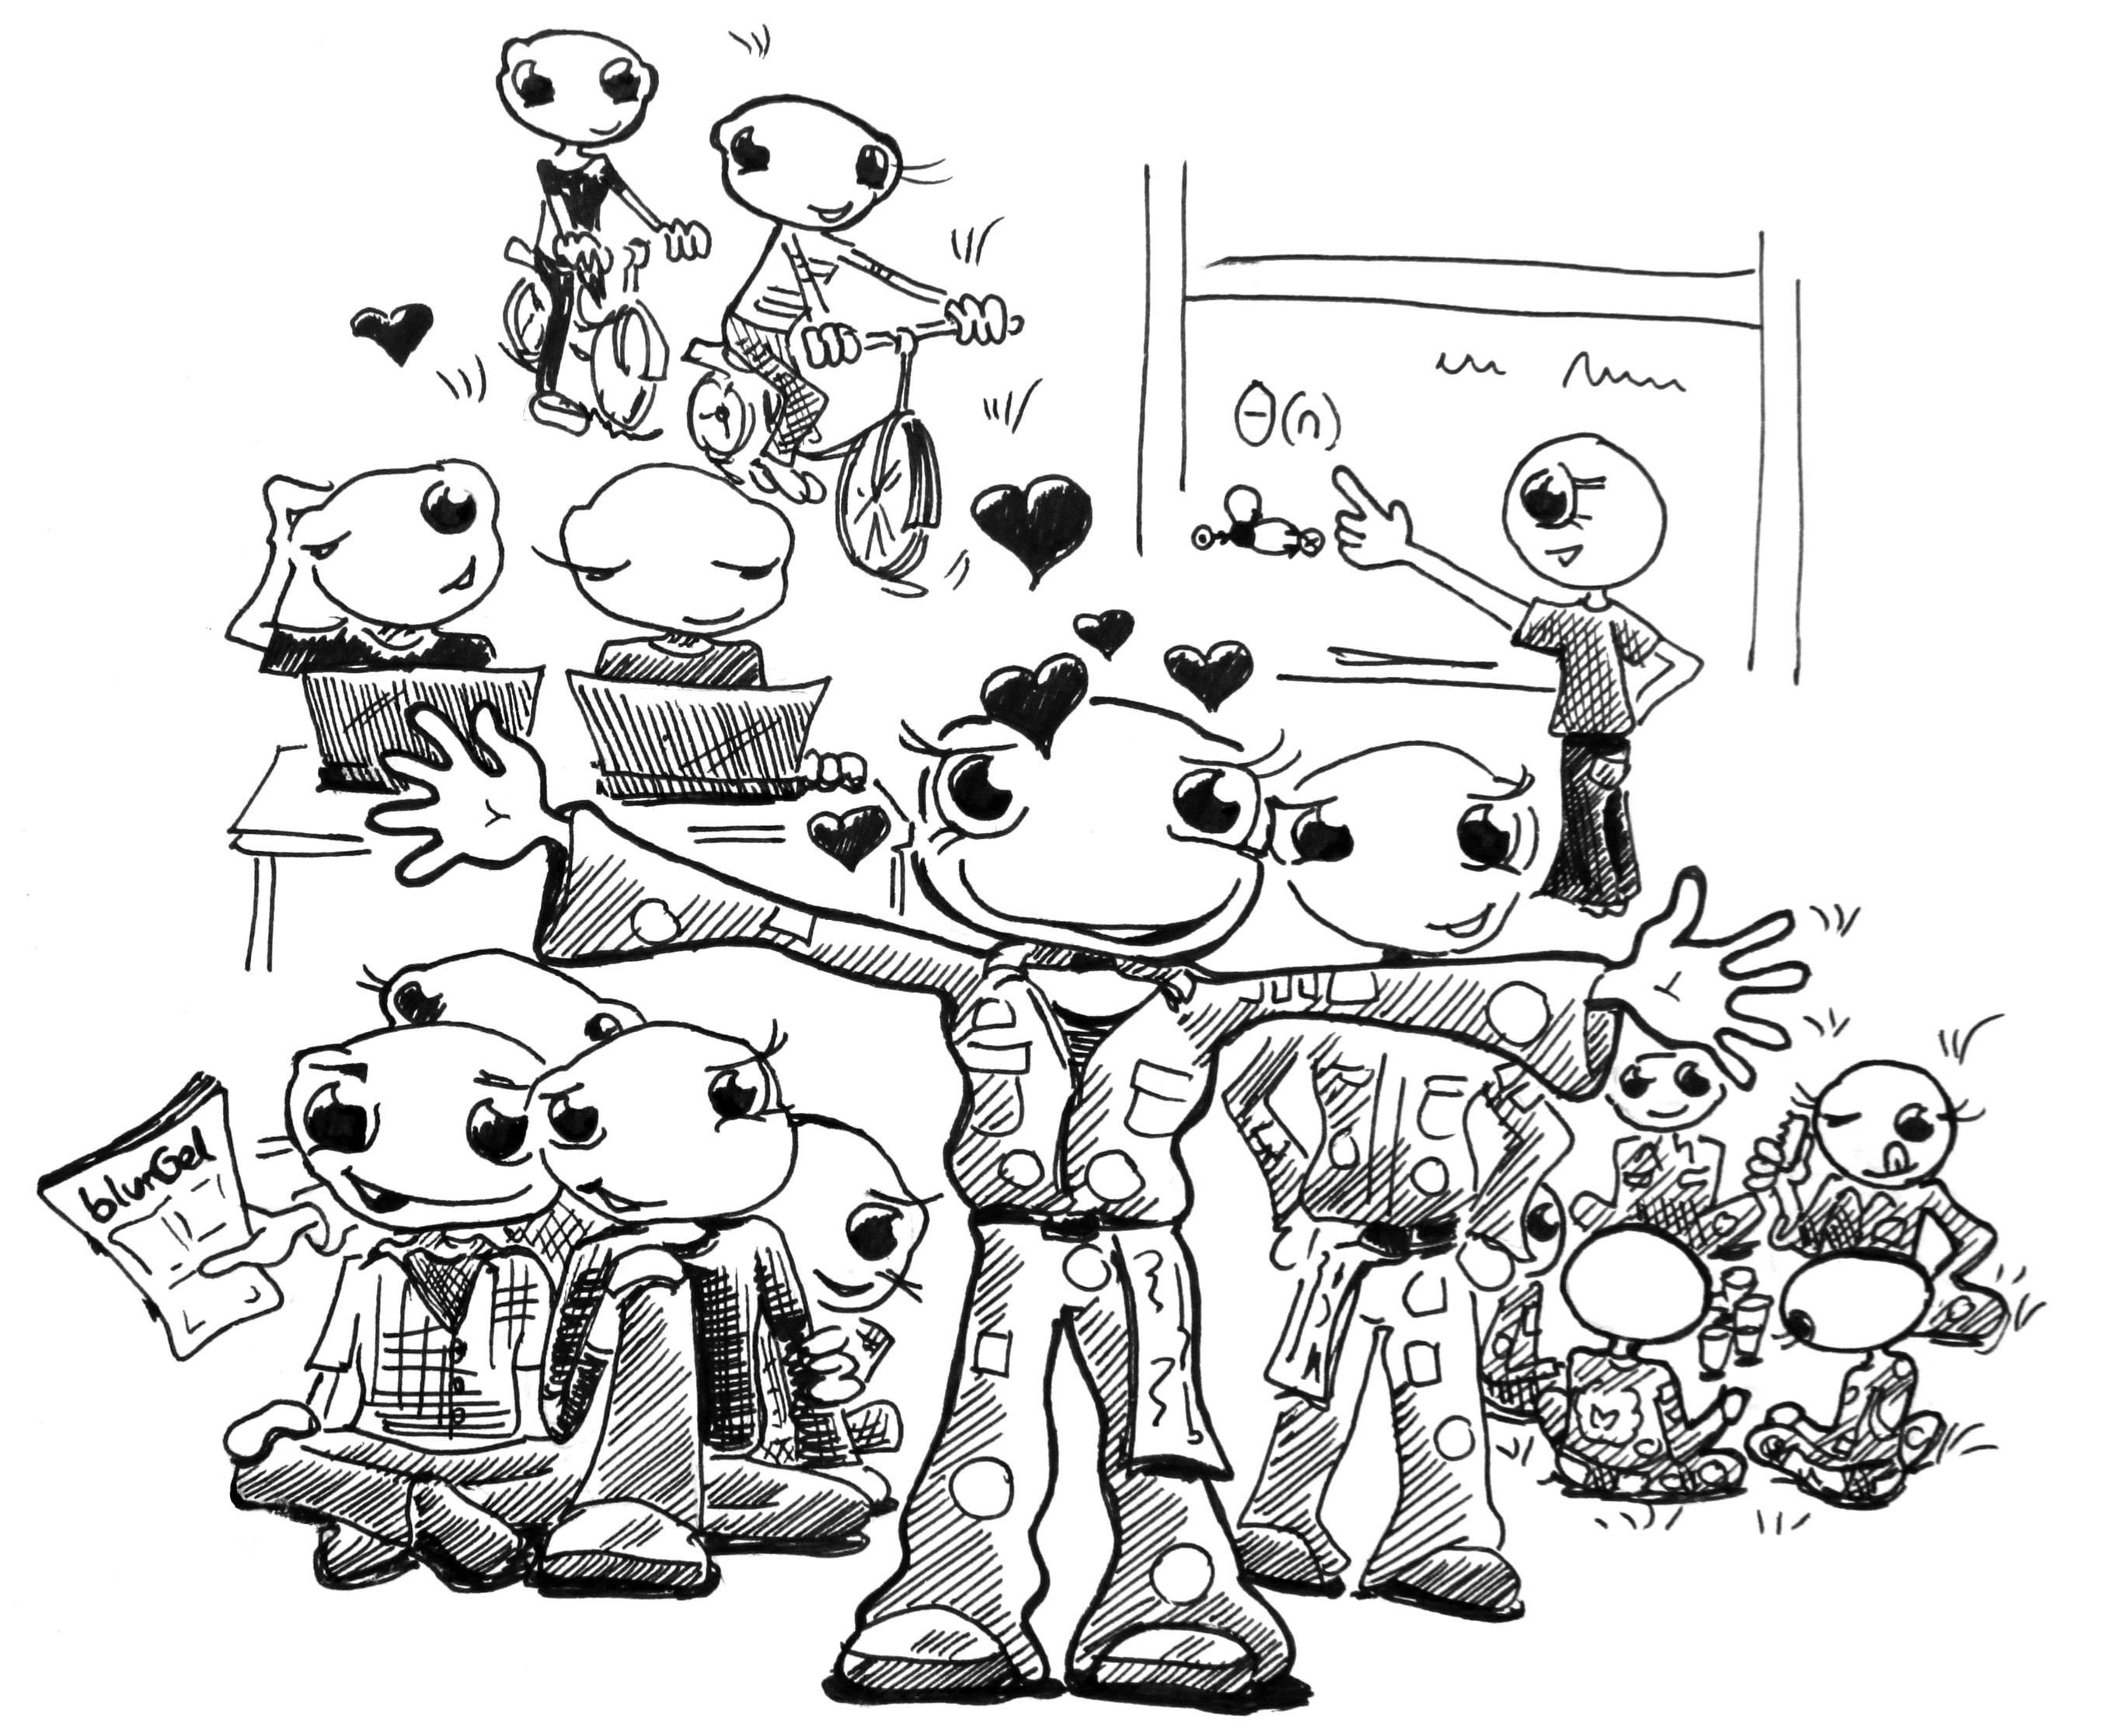
\includegraphics[keepaspectratio,width=\textwidth]{elements/kika.jpg}
\vspace{10pt}\\ Som många andra flyttade jag ifrån min egen familj och
kom ensam till den nya världen på Universitetet.\par
\vspace{10pt}
Denna sida tillägnas till familjen jag fick första dagen på Pollax -
DV familjen.\par
\vspace{10pt}
Tack till alla ni som är min familj - ni har alltid en plats i mitt
hjärta.\par
\vspace{10pt}
/Erika ``Kika'' Wahlberg (fd Westermark),
DV99\\{\footnotesize\textit{PS blurGel är bäst! DS}}
\newpage
\fvisa{WRITE IN C}{When I find my code in tons of trouble}
{\footnotesize\textit{Melodi: Let it be}}\par
\vspace{10pt}
When I find my code in tons of trouble,\\
friends and colleagues come to me,\\
speaking words of wisdom:\\
``Write in C.''\par
\vspace{10pt}
As the deadline fast approaches,\\
and bugs are all that I can see,\\
somewhere, someone whispers:\\
``Write in C.''\par
\vspace{10pt}
Write in C, write in C,\\
write in C, oh, write in C.\\
LOGO's dead and buried,\\
write in C.\par
\vspace{10pt}
I used to write a lot of FORTRAN,\\
for science it worked flawlessly.\\
try using it for graphics!\\
Write in C.\par
\vspace{10pt}
If you've just spent nearly 30 hours\\
debugging some assembly,\\
soon you will be glad to\\
write in C.\par
\newpage
Write in C, write in C,\\
write in C, yeah, write in C.\\
Only wimps use BASIC.\\
write in C.\par
\vspace{10pt}
Write in C, write in C \\
write in C, oh, write in C.\\
Pascal won't quite cut it.\\
write in C.\par
\vspace{10pt}
Write in C, write in C,\\
write in C, yeah, write in C.\\
Don't even mention COBOL.\\
Write in C.\par
\vspace{10pt}
{\footnotesize\textit{Text: Kriston J. Rehberg}}

\vspace{15pt}
\fvisa{DVL's datasång}{Nu ska vi ut och programmera}
{\footnotesize\textit{Melodi: Gärdebylåten}}\par
\vspace{10pt}
Nu ska vi ut och programmera,\\
supa och slås och kompilera.\\
Bränna SUN-stationer, slå en Mac,\\
å spy på IBM. Fy fan!\\
Med blod skall vi skärmen färga,\\
nu äntligen lär ja'.\\
Kunna dra någon riktig nytta\\
AV MIN YXA\par
\vspace{10pt}
{\footnotesize\textit{Text: Erik Wainikka, Björn Persson, Anders Jansson d.ä., Skåne Danne, samtliga ur DVL88 från Umeå}}

\newpage
\fvisa{OM EMACS}{Emacs är en stor koloss}
{\footnotesize\textit{Melodi: Rullan går}}\\
\\
Emacs är en stor koloss.\\
Tugga på, tugga på.\\
Verkar aldrig komma loss.\\
Tugga på, tugga på.\\
För att flytta på ett tecken\\
går två meg i garbage-säcken.\\
Ner i skärmens undre ran’\\
står: garbage collecting, done!\\
\\
Väntar på’n till min pension.\\
Tugga på, tugga på.\\
Emacs gör en Sparcstation\\
Tugga på, tugga på.\\
snabb som en ABC-80.\\
Högprestanda blir så smått i\\
Emacs, den ser säkert till\\
ingen dödtid blir förspilld!\\
\\
Emacs skriven är i Lisp.\\
Tugga på, tugga på.\\
Inget rimmar alls på Lisp.\\
Tugga på, tugga på.\\
Om du in i kärnan trevar\\
finn en gnu som motorn vevar.\\
Den drar Emacs runt för hand!\\
Klart att det går trögt ibland!\\
\\
{\footnotesize\textit{Text: Ingemar Ragnemalm \oldstylenums{1992}}}

\newpage
\fvisa{DET SKA VA' HEMBRÄNT}{Jag har festat mycket, det har inte varit lätt}
{\footnotesize\textit{Melodi: Husvagn}}\par
\vspace{10pt}
Jag har festat mycket, det har inte varit lätt.\\
Blanda vin och whisky, det kan inte vara rätt.\\
Jag har festat på de allra konstigaste sätt,\\
men äntligen jag funnit hur man ska partajja rätt:\par
\vspace{10pt}
Det ska va hembränt, och supa till i några dar.\\
Det ska va hembränt, drick upp det sista ni har kvar.\\
Det ska va hembränt, och svina runt i overall.\\
Det ska va hembränt, drick nu vad ni tål!\par
\vspace{10pt}
I flera år så var vi lite fina där i kanten.\\
Vi smuttade på vinerna men spara aldrig panten.\\
Men sen vi lärde känna våran vackra overall,\\
så super vi nu landet runt på hemgjord alkohol.\par
\vspace{10pt}
Det ska va hembränt ...\par
\vspace{10pt}
Fem små groggar först för att komma igång med festen.\\
Fem små groggar till för att supa ikapp resten.\\
Fem små groggar sen för att kalla det en kväll.\\
Fem små groggar till så sitter vi i fyllecell.\par
\vspace{10pt}
Det ska va hembränt ...\par
\vspace{10pt}
{\footnotesize\textit{Text: Jesper Wilhelmsson, d97}}

\newpage
\fvisa{KOMMANDOTOLKEN}{Far, jag kan inte få upp min kommandotolk}
{\footnotesize\textit{Melodi: Far, jag kan inte få upp min kokosnöt}}\\
\\
Far, jag kan inte få upp min kommandotolk.\\
Alla sätt jag prövat har vart fel;\\
jag har tryckt på knappar, klickat på varje flik,\\
och jag har sagt, “kommandotolk, tack!”,\\
men skärmen är sig lik.\\
\\
Far, jag kan inte få upp min kommandotolk,\\
inte ens med länk till satellit.\\
På varje antenn, har jag satt kopplingssladdar, men,\\
av kommandotolken min syns inte ett skit!\\
\\
Av kommandotolken min syns inte ett ski-i-it!\\
Jag ser bara Emacs, Xfig och Mosaic.\\
Säg, minns du prompten, far?\\
Glöm bort den, är du rar.\\
för av kommandotolken min syns inte ett skit!\\
\\
Far, jag kan inte få upp min kommandotolk,\\
inte ens med nitroglycerin.\\
När jag hade laddat, mycket omsorgsfullt och väl,\\
bortåt jag sprang, sen sa’ det PANG,\\
och Polacksbacken brann ner...\\
\\
Far, jag kan inte få upp min kommandotolk,\\
för jag har ingen hand med dynamit.\\
Av vårt stolta hus, det återstår bara grus,\\
och av kommandotolken min syns inte ett skit!\\
\\
Av kommandotolken min syns inte ett ski-i-it!\\
Allt det andra har blitt lika indefinit (så att säga).\\
Internet står still, vad ska jag ta mig till?\\
Av kommandotolken min syns inte ett skit,\\
ett skit,\\
ett skit,\\
ett skit,\\
Av kommandotolken min syns inte ett ski-i-it!\\
\\
{\footnotesize\textit{Text: Johan Runeson, Nollespexet DVP Uppsala,
    \oldstylenums{1996}\\ \\ (Personligen tycker jag att det ska vara
    ’Fan, jag kan inte...’ /red. anm.)}}

\vspace{15pt}
\visa{DET VAR FEST NER I FOORUM}
{\footnotesize\textit{Melodi: Det var dans bort i vägen}}\par
\vspace{10pt}
Det var fest ner i FooRum på tisdagsnatten.\\
Upp i trappan gick låten av sången och skratten.\\
Det var tjo! Det var tjim! Det var hej!\\
Där satt dataloger och skåla och söp\\
och skråla och skräna tills hemåt de kröp\\
för dudeli dudeli dej. HEJ!\par
\vspace{10pt}
Där var Starka å Åhus å Renat å Bäsk,\\
där var Herrgårds och Pors som ej luktar av mäsk\\
där var OP och lite Mai Tai.\\
Där var Årsta och Vinbärs och liknande klägg,\\
där var Punsch och likör utav lingon och ägg\\
för dudeli dudeli dej. SKÅL!\par
\vspace{10pt}
{\footnotesize\textit{Text: Andreas Gref, dvl90 Uppsala}}

\newpage
\fvisa{ANOTHER GLITCH IN THE CALL}{We don't need no indirection}
{\footnotesize\textit{(sung to the tune of a not so recent Pink Floyd song)}}\par
\vspace{10pt}
We don't need no indirection\\
We don't need no flow control\\
No data typing or declarations\\
Hey! Did you leave the lists alone?\par
\vspace{10pt}
All in all, it's just a pure-LISP\\
function call\par
\vspace{10pt}
We don't need no side effect-ing\\
We don't need no scope control\\
No global variables for execution\\
Hey! Did you leave those args alone?\par
\vspace{10pt}
All in all, it's just a pure-LISP\\
function call\par
\vspace{10pt}
We don't need no allocation\\
We don't need no special nodes\\
No dark bit-flipping in the functions\\
Hey! Did you leave the bits alone?\par
\vspace{10pt}
All in all, it's just a pure-LISP\\
function call
\newpage
We don't need no compilation\\
We don't need no load control\\
No link edit for external bindings\\
Hey! Did you leave that source alone?\par
\vspace{10pt}
All in all, it's just a pure-LISP\\
function call\par
\vspace{10pt}
{\footnotesize\textit{Text: DVLs tidning \#11subscript:8}}

\vspace{15pt}
\fvisa{TUPPENS KLAGOVISA}{Tuppens väckarklocka ringer sex varje morgon}
{\footnotesize\textit{Melodi: Hoppsan vilken dag}}\\
\\
Tuppens väckarklocka ringer sex varje morgon\\
då måste han gå upp till ännu en jävlig dag.\\
Han sätter sig på Teknikum och får genast ångest\\
rysningar i kroppen alla världens obehag.\\
\\
Ännu en föreläsning om fysik och sånt\\
men han tänker på en svettig datasal.\\
Tänk att sitta vid en dator i 1411\\
men miniräknarn är hans enda val.\\
\\
Tuppens verklighet det är ett liv utan glädje\\
gula overaller är ju inget man vill ha.\\
Jag borde ändå gjort som min gamla mamma sa,\\
en DVP:are é va man borde va\\
\revrpt en DVP:are é va man borde va\rpt

\newpage
\null
\vfill
\index{ÃCompiler complaint@\uppercase{Compiler complaint}}
\begin{center}
  \tiny{Compiler complaint}\par
  \vspace{5pt}
  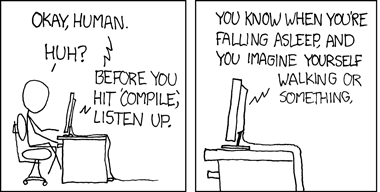
\includegraphics[keepaspectratio,width=0.8\textwidth]{elements/images/compiler_complaint_1.png}\par
  \vspace{5pt}
  \tiny{BY-NC 2.5 xkcd.com}
\end{center}
\par
\vspace{10pt}
\vfill
\null
\newpage
\visa{SOMMARHACK}
{\footnotesize\textit{Melodi: Sommarnatt}}\par
\vspace{10pt}
Sommarhack - när jag sitter vid min PC - aha.\\
Sommarhack - vid min jättemaskin.\\
Sommarhack - när jag är i PULets mörker - aha.\\
Sommarhack - ger en skön SUP1 feeling.\par
\vspace{10pt}
IBM med MS-DOS, i ’89-års modell.\\
Jag öser på för fullt med \\
Word, och Microsoft Excel.\\
Jag sveper fram med musen, ja jag\\
klickar snabbt på knappen.\\
Det är så skönt att sitta här och\\
dubbelklicka i natten\par
\vspace{10pt}
Sommarhack...\par
\vspace{10pt}
Det är en ganska enkel sak\\
å få min kod till att exekvera.\\
En enda liten kompilering, ja förresten\\
det kan bli flera.\\
I datorns vilda RAM-minne, ja där\\
trivs jag allra bäst.\\
Det gäller bara COBOL-kod,\\
och vem som hackar mest!\par
\vspace{10pt}
Sommarhack...

\newpage
\fvisa{NER I MIN KÄLLARE}{De flesta gillar väl fester}
{\footnotesize\textit{Melodi: Ner i min källare}}\par
\vspace{10pt}
De flesta gillar väl fester, att umgås på nått sätt.\\
Och ofta när man har gäster så dricker man en skvätt.\\
Men skulle det då hända, att spriten den tar slut,\\
Långt innan gästerna är på väg ut.\\
\\
Då går jag ner i min källare, där lever man sällare,\\
för där har jag kvar min gamla kokare. \textit{*tuut, tuut*}\\
Jag kokar mäsken om kvällarna och häller i buteljerna \\
och spriten blir fin i ångan från maskin.\\
\\
Så hände det då i helgen att gästerna som kom, \\
min inställning till buteljen de inte tyckte om.\\
De prata' om maskinen som inte laglig var\\
jag får nog ligga lågt i några dar.\\
\\
Så jag går ner i min källare, där lever man sällare...\\
\\
På måndan kom sen polisen, oj det var inte bra.\\
Han hade hört några rykten och undra vad det var.\\
Men snuten verkade trevlig, med festarsugen min.\\
Jag öppnade min dörr och sa: stig in!\\
\\
Så gick vi ner i min källare, där lever man sällare...
\par
\vspace{10pt}
{\footnotesize\textit{Text: Jesper Wilhelmsson, d97}}

\newpage
\fvisa{IT IS FREE}{When I find myself in front of Windows}
{\footnotesize\textit{Melodi: Let It Be}}\par
\vspace{10pt}
When I find myself in front of Windows,\\
Father Torvalds comes to me,\\
Speaking words of Linux, ``It is free!''.\\
And when hackers crack my system\\
through some strange NT obscurity,\\
he gives me the source-code, ``It is free!''.\par
\vspace{10pt}
It is free, it is free, it is free, it is free.\\
Linux is the answer, and it's free.\par
\vspace{10pt}
When the broken system crashes\\
and blue screens of death I see.\\
There is one true rescue, and it's free.\\
For though there may be doubts first\\
it will sure bring life to your PC\\
`Cause Linux is the answer, and it's free.\par
\vspace{10pt}
It is free, it is free, it is free, it is free,\\
You even get the source-code, it is free.\par
\vspace{10pt}
In the darkest night, when hacking,\\
Xfree stares right back at me,\\
Now I've installed Linux, I feel free.\\
No longer mad with my computer,\\
No more does it crash on me\\
Now I've installed Linux, it is free.
\newpage
It is free, it is free, it is free, it is free,\\
Open-sourced true power, it is free.\par
\vspace{10pt}
{\footnotesize\textit{Text: David Weinehall}}

\vspace*{-10pt}
\newpage
\fvisa{C-Sången}{Se hit kära vänner, Ni alla oss känner}
{\footnotesize\textit{Melodi: Sovjetunionens nationalsång}}\par
\vspace{10pt}
Se hit kära vänner, Ni alla oss känner,\\
det är vi som går här i blå overaller.\\
Den bästa sektionen som finns här på jorden.\\
Höjer nu glasen så tar vi en skål.\par
\vspace{10pt}
\revrpt För våran kära C-sektion\rpt\\
Den bästa sektionen som finns på vår jord.\\
\revrpt Se, se här kommer C-sektionen\rpt\\
Se upp kära vänner, för här kommer vi.\par
\vspace{10pt}
Från öster till väster, från norr eller söder.\\
I studier som fester förenen er bröder.\\
Sjungen nu alla låt C-sången skalla.\\
Höjen nu glasen, ta ännu en skål.\par
\vspace{10pt}
För våran kära C-sektion...\par
\vspace{10pt}
{\footnotesize\textit{Linköpings C-sektions sång. \\
					 C-sektionen lades ner 2014, så avsluta denna sång med en gravöl}}


\newpage
\fvisa{ODE TILL PROLOG}{Vår professor sa så här}
{\footnotesize\textit{Melodi: Ovan där}}\par
\vspace{8pt}
Vår professor sa så här\\
Ni ska inte ha besvär\\
Med begin och end och for och goto,\\
Fortran, och sånt där!\\
Jag har sett i en vision\\
att i änglakörens ton\\
finns ett inslag\\
för den rätta tron\par
\vspace{7pt}
OVAN DÄR\\
hackar dom Prolog\\
och dom dricker Coke ur stora tråg\\
ja, jag nästan spricker av löftet som jag fått:\\
Varje Prolog-hacker måste få det gott.\par
\vspace{7pt}
LM Ericsson sa då,\\
vi kan inte alls förstå\\
varför dom som kunde Fortran plötsligt\\
blivit har så få!\\
Ja, visst är det något stort\\
just det där som ni har gjort\\
``But when it comes to business boys''\\
måste det gå Fort!!\par
\vspace{7pt}
OVAN DÄR\\
hackar dom Prolog\\
och dom dricker Coke ur stora tråg\\
Ovan där\\
där får vi vara med,\\
utom dom där nere, dom som kunde C!

\vspace*{-10pt}
\newpage
\fvisa{Nu har DV:arna kalas}{Lyft ditt välförsedda glas}
{\footnotesize\textit{Melodi: Ding Dong Merrily on High}}\par
\vspace{10pt}
Lyft ditt välförsedda glas,\\
det är en härlig börda!\\
Nu har DV:arna kalas,\\
vi segern snart skall skörda.\\
\\
Ding dinge dinge ding, dinge dinge ding\\
dinge dinge ding dong dong\\
i morgon är det lördag.\\
\\
Sätt nu glaset till din mun,\\
se döden på dej väntar.\\
Nu har grabbarna kalas,\\
hör liemannen flämtar.\\
\\
Ding dinge dinge ding, dinge dinge ding\\
dinge dinge ding dong dong\\
Begravningsklockor klämtar.

\newpage
\fvisa{VANDRANDE RODNAD}{Ingen har sett en sådan Hallands fläder}
{\footnotesize\textit{Melodi: Fantomens brallor}}\par
\vspace{10pt}
Ingen har sett en sådan Hallands fläder\\
rester av kor och smak utav fjäder\\
stark är den som en tunnelborr\\
ge mig mera för min stupe är torr\par
\vspace{7pt}
Vandrande rodnad kliar under sviden\\
sticker i ben och armar hela tiden\\
pröva en snaps med spår av Rhoca-Gil\\
det är bättre än en nervgasmissil\par
\vspace{7pt}
Händerna skakar, nerverna rycker\\
jag skiter blankt i vad andra tycker\\
visst får man skaffa sig rullstol\\
men jag känner mig i alla fall cool\par
\vspace{7pt}
Vandrande rodnad ...\par
\vspace{7pt}
Bindor, tamponger, glöm det flickor\\
Hallands är inte som andra drickor\\
har sina sidor på många sätt\\
men jag lovar att ni håller tätt\par
\vspace{7pt}
Vandrande rodnad ...\par
\vspace{7pt}
Kroppen min har nu bränts till aska\\
jag skulle nog inte tömt din flaska\\
Jag trodde ju aldrig när du bjöd \\
att det skulle bli bleka död.\par
\vspace{7pt}
Vandrande rodnad ...\par
\vspace{10pt}
{\footnotesize\textit{Text: Anders Ramsell, Johan Runeson, Henrik Eriksson}}

\vspace*{-11pt}
\newpage
\visa{Ljusblå - är vår overall}
{\footnotesize\textit{Melodi: Jul, jul, strålande jul}}\par
\vspace{10pt}
Ljus - blå\\
Är vår overall\\
Ljusblå är ock spegaten\\
Gult lyser stjärnor\\
Våra C:n likaså\\
De är symbolen för linjen vi gå\\
Teknisk datavetenskap\\
Det är vår linje, den är ju ett kap\par
\vspace{10pt}
Ljus - blå\\
Är vår overall\\
Ljusblå så in i Norden...
\par
\vspace{10pt}
{\footnotesize\textit{Till minne av C-sektionen i Linköping\\ Text: Daniel Holmgren, C96. Framförd av Richard Lönneborg, C97, och Holm på Pirayas G\&G anno 1997}}

\vspace{15pt}
\fvisa{Köpesprit vill vi ej ha}{På sittningen så träffa jag en tjej från samma byggd}
{\footnotesize\textit{Melodi: Snickerboa}}\par
\vspace{10pt}
På sittningen så träffa jag en tjej från samma byggd\\
En trevlig flicka som fick smaka på min goda bryggd\\
HB är vi uppväxta på\\
Vi super tills vi ej kan gå\\
Köpesprit vill vi ej ha\\
Närproducerat ska de va'\par
\vspace{10pt}
{\footnotesize\textit{Text: Patrik Broman}}

\newpage
\visa{MORS LILLA DATOR}
{\footnotesize\textit{Melodi: Mors lilla Olle}}\par
\vspace{10pt}
Mors lilla dator åt skogen gick,\\
mitt i programmet så sade det klick\\
svart bidde skärmen och minnet försvann,\\
den informationen kan ingen få fram.\par
\vspace{10pt}
Brummeli-brum vad brummar där?\\
Det sprakar och gnistrar, ett jordfel det är!\\
Blixtarna blå ifrån burken det slå,\\
synd att jag nu här ensammen stå.\par
\vspace{10pt}
Hyscheli-hysch vad prasslar här?\\
Fram väller pappret ur printern där!\\
Den har fått nippran av tecken så små,\\
jag tror att jag snart hemåt skall gå.

\vspace{15pt}
\visa{Om du inte dricker bäsken}
{\footnotesize\textit{Melodi: Deck the halls}}\par
\vspace{10pt}
\par
Om du inte dricker bäsken\\
Falalalala lala lala\\
Då får du en smäll på käften\\
Falalalala lala lala\\
Töm den nu\\
utan strul\\
för det är ju inte jul\\
om du inte dricker bäsken\\
Falalalala lala lala
\vspace{10pt}
{\footnotesize\textit{Text: Patrik Broman}}

\vspace*{-10pt}
\newpage
\visa{Jag trivs bäst i overallen}
{\footnotesize\textit{Melodi: Jag trivs bäst i öppna landskap}}\par
\vspace{10pt}
\par
Jag trivs bäst i overallen\\
overallen är mitt hem\\
Den skyddar hela kroppen min\\
speciellt min kära lem\\
Jag trivs bäst i overallen\\
den doftar friskt och fräscht\\
Man undrar dock varför ingen\\
är av färgen beige\\
\vspace{10pt}
I utbyte mot kroppsvätskor\\
man byter delar hit och dit\\
Super hejdlöst varje dag\\
och rullar sig i skit\\
Jag trivs bäst i overallen\\
overallen är mitt hem
\vspace{10pt}
{\footnotesize\textit{Text: Patrik Broman}}

\newpage
\visa{Lille OLLe}
{\footnotesize\textit{Melodi: Katjuscha}}\par
\vspace{10pt}
Lille Olle skulle gå på disco\\
men han hade inte någon sprit.\\
Lille Olle fixa lite hembränt,\\
Lille Olle gick då på en nit.\par
\vspace{10pt}
Lalala…\par
\vspace{10pt}
Lille Olle skulle börja festa,\\
spriten blandade han ut med MER.\\
Lille Olle drack upp hela bålen,\\
Lille Olle ser nu inte mer.\par
\vspace{10pt}
Lille Olle skaffade en ledhund,\\
den var ful och även ganska trind.\\
Olles ledhund drack upp femton flaskor,\\
Olles ledhund är nu också blind.\par
\vspace{10pt}
Lille Olle började med droger,\\
blandade ut sin LSD med juice.\\
Lille Olles hjärna stod i lågor,\\
Lille Olle dog av överdos.\par
\vspace{10pt}
Lille Olle sitter nu i himlen,\\
festa kan man även göra där.\\
Lille Olle skaffade en ölback,\\
capsar nu med Gud och Sankte Per.\par
\vspace{10pt}
{\footnotesize\textit{Text: Calle Isaksson}}

\newpage
\fvisa{Datavetarkandidat}{För länge sen}
{\footnotesize\textit{Melodi: Teddybjörnen Fredriksson}}\par
\vspace{10pt}
För länge sen\\
ca 2007\\
fick jag en plats på DVK\\
Det kändes rätt\\
här trivs jag jättebra\\
bästa programmet man kan gå\par
\vspace{10pt}
Datavetarkandidat\\
ja, jag är en sån\\
festar hela natten lång\\
och jag slutar ej imorn\\
Datavetarkandidat\\
min overall den luktar skit\\
men jag är ändå jätteglad att jag äntligen hittat hit\par
\vspace{10pt}
Ingen vet\\
om jag examen tar\\
DVK är nu mitt andra hem\\
Det kanske sker\\
en vacker sommardag\\
att jag får en plats på DVM\par
\vspace{10pt}
Datavetarkandidat...\par
\vspace{10pt}
{\footnotesize\textit{Text: Patrik Broman}}

\newpage
\fvisa{Overallen}{Det finns ett alldes särskilt plagg}
{\footnotesize\textit{Melodi: Hallelujah}}\par
\vspace{10pt}
Det finns ett alldes särskilt plagg \\
det bästa om man vill få ragg\\
man blir så jävla snygg i overallen\\
Om du är yngst eller äldst\\
du kan ha den till vad som helst\\
på alla fester passar overallen\par
\vspace{7pt}
Overallen\\
Overallen\\
Overallen\\
Overallen\par
\vspace{7pt}
Ett ärrat plagg min ove är\\
ett märke här en spya där\\
Det ska synas att man använt overallen\\
Om overallen luktar pung\\
det gör inget håll dig lugn\\
ingen luktar gott i overallen\par
\vspace{7pt}
Overallen...\par
\vspace{7pt}
I oven händer mycket kul\\
om du är snygg eller ful\\
Det spelar ingen roll i overallen\\
för i oven är man alltid snygg\\
i oven kan man vara trygg\\
när man springer runt i overallen\par
\vspace{7pt}
Overallen...\par
\vspace{10pt}
{\footnotesize\textit{Text: Patrik Broman}}

\vspace*{-10pt}
\newpage
\visa{BITTAR OCH BAJTAR}
{\footnotesize\textit{Melodi: Diggiloo Diggiley}}\par
\vspace{10pt}
Bittar och bajtar,\\
magiska sajter!\\
Plötsligt en dag har det hänt -\\
å vilken tur,\\
jag är en ljusbblå figur!\par
\vspace{10pt}
En da i labbet,\\
jag satt där och hacka.\\
Sprang i väg till fiket\\
och köpte mig en macka\\
Väl tillbaka i labbet,\\
fann jag en underbar länk!\par
\vspace{10pt}
Http, www, cs, umu, se -\\
ja det är den adressen man ska ha\\
när man surfar runt på nätet,\\
det gör jag varje dag.\par
\vspace{10pt}
Http, www, cs, umu, se -\\
det är bara hänga med, ta ton!\\
Å jag börjar nästan sväva\\
vid min Sparc-station.\par
\vspace{10pt}
{\footnotesize\textit{Text: Mest Holm, C96, och Nico, C95,\\
under en overallspåtarkväll hos dåvarande ordförande Vickan, C95, inför linjekonferensen -97 i Uppsala}}

\newpage
\fvisa{DVrecceskålen}{Välkomna alla reccar små}
{\footnotesize\textit{Melodi: Snickerboa}}\par
\vspace{10pt}
Välkomna alla reccar små\\
Välkomna till DV\\
På eran kanske första gasque\\
vi lär er denna sed:\\
Först till kavaljeren en skål\\
och vänd dig sen mot nästa mål\\
Till sist så tar du framåt en titt\\
och tar en smutt av glaset ditt\par
\vspace{10pt}
Och nu är halva skålen klar\\
Det var väl ganska lätt?\\
Då vänder vi på ordningen\\
ja som en fläskkotlett\\
Först mittemot som ni nyss gjort\\
Nu borde resten gå som smort\\
Som avslutning på denna sång\\
så praktiserar vi en gång!\par
\vspace{10pt}
{\footnotesize\textit{Text: Patrik Broman}}

\newpage
\index{ÃEn hälsning från historien@\uppercase{En hälsning från historien}}
\section{En hälsning från historien}\vspace{10pt}
\setlength{\parindent}{15pt}
\noindent\hspace{15pt}Den 18 november 1994 samlades representanter för
Sveriges tre magisterutbildningar i datavetenskap utanför Linköping
(det legendariska 100-köret skulle hållas dagen efter) för
genomsjungning av den nya gemensamma sångboken Manualen. Det var ett
ambitiöst projekt, det skulle vara den största och mest kompletta
samlingen av sånger, och för första gången hade vi samarbetat
(mestadels lett från DV i Umeå) och framställt denna viktiga, samlande
sak: en egen sångbok!

Den versionen av Manualen skulle sedan komma
att tryckas om, bli föremålet för en mindre skandal i Umeå, spridas
vidare över landet men framför allt användas. Det sjungs mycket hos
oss datavetare, och Manualen fanns och finns ständigt framme för att
stödja sjungandet av både kända och okända sånger.

Och nu är det dags igen. En ny Manualen-komitté
har kört hela vägen in i kaklet och gjort en ny utgåva, så att nya
generationer av Datavetare, i Uppsala och annorstädes kan på nytt
sjunga Emacs-visan(?), O Gamla Klang och Calmarevisan både rätt och
starkt. Tack och Grattis till dem!

Av olika anledningar råkade det ligga en 10-15
oanvända Manualer från 1.0 och 1.1-tryckningarna hemma hos mig, och
när det Manualens 20-årsjubileum vankades i november 2014 så
beslutades det snabbt att dessa a) skulle spridas till nya
generationer samt b) inkomsten från denna spridning skulle gå direkt
till nya Manualen. Så blev det. Tack till alla som slog två flugor i
en smäll och både fick en liten och obetydlig del av historien i sin
ägo, samt bidrog till den nya och betydliga framtidens
sångböcker. Trevligt var det också.

Från Manualen 1.0-komittén (Mig själv Måns,
Nenne + andra): Grattis till den nya komittén samt till DIG! som just
läser detta och uppenbarligen innehar denna nya Manual. Slit den med
hälsan, och sjung mycket! Det är den värd!\par
\vspace{10pt}
\noindent Spånga 3 juli 2015\\
Måns af Klercker, d93mkl\par
\setlength{\parindent}{0pt}
\vfill
\begin{center}
  \noindent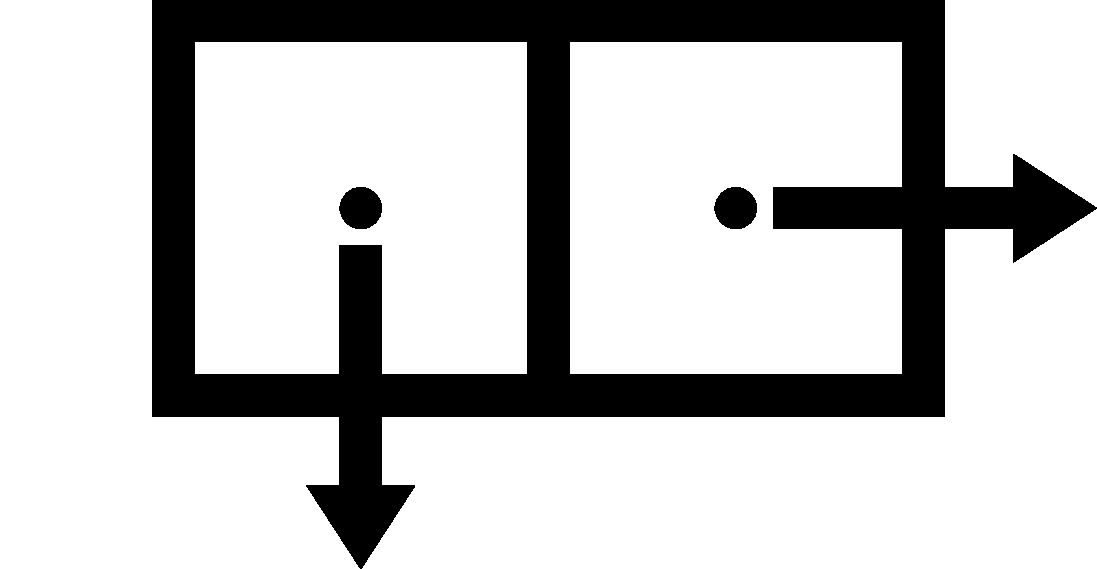
\includegraphics[keepaspectratio,width=0.6\textwidth]{elements/consbox.pdf}
\end{center}
\vfill
\null
\newpage
\visa{LÄNKA LILLA DATOR DÄR}
{\footnotesize\textit{Melodi: Blinka lilla stjärna där}}\par
\vspace{10pt}
Länka lilla dator där,\\
hur jag undrar hur du är,\\
ständigt frestar du mitt mod,\\
med en massa fel i kod.\\
Blinka lilla dator kär,\\
vad jag undrar hur du gör.\par
\vspace{10pt}
När den sköna sol blitt släckt,\\
strax du startas upp så käckt.\\
Börjar klar din stilla gång,\\
glimmar, glimmar natten lång.\\
Länka lilla dator kär,\\
jag undrar vad klockan är.

\vspace{15pt}
\fvisa{PROGRAMFÖRKLARING}{Dataloger är bättre än andra}
{\footnotesize\textit{Melodi: Vers 1, 2 \& 6 Gamla Nordsjön; 3, 4 \& 5 Rudolf med röda mulen}}\par
\vspace{10pt}
Dataloger är bättre än andra\\
detta märks inte minst på en fest\\
Det finns vissa man aldrig skall klandra\\
och bland dessa är Uppsalas bäst\par
\vspace{10pt}
Vi kalas från kalas hemåt vandra\\
nästan alltid tillsammans med gäst\\
Att vi plägar se ner på er andra\\
är helt rättvist, vi är trots allt bäst\\
\\
Se vackra datalogen\\
i sin röda overall\\
alltid lika glad i hågen\\
dricker mer än vad ni tål\par
\vspace{10pt}
Pilsner är partydrycken\\
CC, det är vardagsmat\\
Hackers, de klarar rycken\\
det är inte bara prat\\
\\
Snyggast, smartast, vackrast, bäst\\
Käck med elegans\\
Trevlig, ödmjuk och modest\\
Alla andra saknar chans\par
\vspace{10pt}
Detta kan verka skryt, men är sanning\\
Kan bevisas med hjälp av Prolog\\
Därför uppmanar vi till ett kraftfullt HURRA!\\
Vi ÄR datavetenskap.
\par
\vspace{10pt}
{\footnotesize\textit{Text: Andreas Gref, Pär Mattson och Gustaf Naeser\\
Eposet nedtecknades på väg hem från 100-köret 1994.}}

\newpage
\fvisa{THE FREE SOFTWARE SONG}{Join us now and share the software}
{\footnotesize\textit{Melodi: Sadi moma bela loza}}\par
\vspace{10pt}
Join us now and share the software;\\
You'll be free, hackers, you'll be free.\\
Join us now and share the software;\\
You'll be free, hackers, you'll be free.\par
\vspace{10pt}
Hoarders can get piles of money,\\
That is true, hackers, that is true.\\
But they cannot help their neighbors;\\
That's not good, hackers, that's not good.\par
\vspace{10pt}
When we have enough free software\\
At our call, hackers, at our call,\\
We'll kick out those dirty licenses\\
Ever more, hackers, ever more.\par
\vspace{10pt}
Join us now and share the software;\\
You'll be free, hackers, you'll be free.\\
Join us now and share the software;\\
You'll be free, hackers, you'll be free.

\newpage
\visa{DV:s Reccar}
{\footnotesize\textit{Melodi: Midnatt råder}}\par
\vspace{10pt}
DV:s reccar sitter här på gasquen \\
mikrogasquen\\
Kanske längtar fram till kaffekasken\\
kaffekasken\par
\vspace{10pt}
Datavetarkandidater capsar\\
varje kväll\par
\vspace{10pt}
DV:s reccar undrar vad som luktar\\
vad som luktar\\
DV:s faddrar reccen sedan tuktar\\
sedan tuktar\par
\vspace{10pt}
Datavetarkandidater luktar\\
overall\par
\vspace{10pt}
DV:s reccar vet ej vad som väntar\\
vad som väntar\\
Reccen vaknar bakfull, trött och flämtar\\
trött och flämtar\par
\vspace{10pt}
Datavetarkandidater börjar\\
hacka C\par
\vspace{10pt}
{\footnotesize\textit{Text: Patrik Broman}}

\newpage
\fvisa{HANDELSVISA}{Vi vill aldrig gå på Handels}
{\footnotesize\textit{Melodi: O hur saligt att få vandra (Sv. Ps. 300)}}\par
\vspace{10pt}
\par
Vi vill aldrig gå på Handels,\\
Aldrig tenta företagsekonomi.\\
Deras IQ den e' Mandels\\
Och förståndet, det har ju gjort sorti.\\
Dom har jätteusla snören,\\
Till sitt jätteusla draperi.\\
Dom kan bara räkna ören,\\
Hela skolan e' ett enda aperi!\par
\vspace{10pt}
Handels är skit - Jag vill ej dit...\par
\vspace{10pt}
Mammons pojkar är dom alla,\\
Pappas flickor är dom likaså,\\
Går och tror att dom är balla,\\
Fastän dom inget alls ju förstå.\\
Hela Handels borde rivas,\\
Detta anser hela vårat lag.\\
Då skulle datavetarn' trivas\\
Uppå denna Handels ljuva domedag!\par
\vspace{10pt}
Åh, vilket drag - på denna dag...\par
\vspace{10pt}
{\footnotesize\textit{Text: Team kangaroo Gerhards-gasque 1977}}

\newpage
\fvisa{DATAVETARNAS PARADMARCH}{Ja, här kommer datavetare}
{\footnotesize\textit{Melodi: Fritjof Anderssons paradmarch}}\par
\vspace{10pt}
Ja, här kommer datavetare\\
med märken på vår dräkt.\\
Vi knappar kod, \\
vi hackar LISP\\
och surfar runt på nätet.\par
\vspace{10pt}
Vi lämnar pöbeln stående\\
och gapande förskräckt.\\
Det vi inte kan, \\
det kan ingen ann -\\
nu går vi upp i labbet.\par
\vspace{10pt}
Och när vi loggat ut,\\
ja då går vi på någon fest\\
och tar oss några bira,\\
för det gillar vi ju bäst!\par
\vspace{10pt}
För där är där vi inte är\\
och här är där vi är!\\
Vi knappar kod,\\
vi hackar LISP\\
och festar runt Sverige.\par
\vspace{10pt}
{\footnotesize\textit{Text: Selander, C93 \& Daniel ``Holm''
    Holmgren, C96.\\ Skrevs i baksätet på en Toyota Camry, på väg
    till linjekonferensen -97 i Uppsala. Omdöpt av Jubileumsgruppen
    inför 30 år jubiléet i Uppsala}}

\newpage
\visa{Photoshop}
{\footnotesize\textit{Melodi: Sudda bort din sura min}}\par
\vspace{10pt}
Det var en gång en pojke/flicka som jämt var snäll och glad\\
Men så kom generalen och frågade en dag\\
Om hen ville bli en mottagningsrekåit\\
Och pojkens/flickans glada dagar då för evigt var förbi\par
\vspace{10pt}
(För då sa generalen)\par
\vspace{10pt}
Scanna in och retuschera bort ditt fula flin\\
Scanna in och retuschera bort ditt fula flin\\
Munnen ska va' spikrak och bestämd\\
Minen alltid butter och beklämd\\
Munnen har du fått att kommendera (reccar)\\
Retuschera bort ditt fula flin\par
\vspace{10pt}
Och snart kom lilla reccen till stora UTN\\
Och aldrig rekåiten fick le när dom såg på\\
När reccen festa' runt gick hen ensam varje kväll\\
För är man rekåit ska man va' nykter och formell\par
\vspace{10pt}
(För general säger)\par
\vspace{10pt}
Scanna in och retuschera bort ditt fula flin...\par
\vspace{10pt}
{\footnotesize\textit{Original text: CQ98 Peter, Magnus; Fulhackad av: Lukas Klingsbo DV09}}

\newpage
\fvisa{MUNKAR}{Jag vill ha munkar}
\vspace{10pt}
Jag vill ha munkar, munkar, munkar med hål i,\\
stora feta munkar med hål i.\\
När jag kommer hem till dig\\
så vill jag inte ha nå'n leverpastej.\par
\vspace{10pt}
Jag vill ha nunnor, nunnor, nunnor med hål i,\\
stora feta nunnor med hål i.\\
När jag kommer hem till dig\\
så vill jag inte ha nå'n leverpastej.\par
\vspace{10pt}
Jag vill ha kramar, kramar, kramar med tryck i,\\
stora mjuka kramar med tryck i.\\
När jag kommer hem till dig\\
så vill jag inte ha nå'n leverpastej.\par
\vspace{10pt}
Jag vill ha kyssar, kyssar, kyssar med sug i,\\
stora blöta kyssar med sug i.\\
När jag kommer hem till dig\\
så vill jag inte ha nå'n leverpastej.\par
\vspace{10pt}
{\footnotesize\textit{Kallas även 0-ans sång, då 0-orna tvingas sjunga denna under 0-ningen på Teknisk Datavetenskap vid Umeå universitet.}}

\newpage
\fvisa{Datanörd}{Se där, han sitter vid sin dator hela natten}
{\footnotesize\textit{Melodi: Waterloo}}\par
\vspace{10pt}
Se där, han sitter vid sin dator hela natten\\
Och där, han surfar runt på Internet och söker efter nå'n\\
Men hittar han någon, å nej\\
Han längtar så efter en tjej\par
\vspace{10pt}
Datanörd, stirrar på skärmen helt oberörd\\
Datanörd, skriver man C blir man helt förstörd\\
Datanörd, UNIX-passionen är oerhörd\\
Datanörd, han är en tönt, ja en datanörd\\
W W W, en datanörd, han är en tönt, ja en datanörd\par
\vspace{10pt}
Se där, hon sitter ensam i ett hörn av baren\\
Hon ler, mot honom men han vågar inte ta\\
den chans han fått\\
De'e lättare titta i smyg\\
Han är ju så otroligt blyg\par
\vspace{10pt}
Datanörd, stirrar på skärmen helt oberörd ...\par
\vspace{10pt}
Men så, en dag han fick en ovve med consbox på\\
Och så, en mössa och se'n solglasögon, svarta som en natt\\
Så blev till sist en charmör\\
Och tjejerna smälter som smör\par
\newpage
General, ingen ser genom hans hårda skal\\
General, makten han har är den helt global\\
General, alltid på TV i var kanal\\
General, han är hjälte vår general\\
Se, se, se, vår general, han är en hjälte vår general\par
\vspace{10pt}
{\footnotesize\textit{Text: CQ98 Peter Johansson \& Magnus Lundqvist\\
Reviderad av Manualen 2015-gruppen i Uppsala}}

\vfill
\index{ÃGOTO@\uppercase{GOTO}}
\begin{center}
  \tiny{GOTO}\par
  \vspace{5pt}
  
\includegraphics[keepaspectratio,width=0.8\textwidth]{elements/images/goto_2.png}\par
  \vspace{5pt}
  \tiny{BY-NC 2.5 xkcd.com}
\end{center}
\par
\vfill
\chapterpageimage{Snapsvisor}{Snapsvisor}{elements/snaps.jpg}
\tvisa{SUPARNAS ORDNING}
\vspace{8pt}
\begin{enumerate}[leftmargin=0.65cm,topsep=0pt,itemsep=2pt,partopsep=0pt,parsep=3pt]
  \begin{minipage}{0.45\linewidth} 
  \item Helan
  \item Halvan
  \item Tersen.
  \item Kvarten
  \item Kvinten
  \item Sexten
  \item Septen
  \item Rivan
  \item Rafflan
  \item Rännan
  \end{minipage}
  \begin{minipage}{0.55\linewidth}
  \item Smuttan
  \item Smuttans unge
  \item Femton droppar
  \item Lilla Manasse
  \item Lilla Manasses Broder
  \item Klämtaren
  \item Kreaturens återuppståndelse
  \item Den bleka dödens dryck
  \item Krokofanternas intåg
  \item Ett evigt liv
  \end{minipage}
\end{enumerate}\par

\vspace{15pt}
\tvisa{ANVISNINGAR FÖR SNAPSENS TAGANDE}
\vspace{10pt}
\begin{itemize}[leftmargin=0cm,topsep=0pt,itemsep=2pt,partopsep=0pt,parsep=3pt,label={}]
\item Snapsen tages till fisk.
\item All mat är fisk, förutom ölsupa och pannkaka.
\item Den som äter ölsupa eller pannkaka, sup på grannens fisk.
\item Skulle grannen förtära ölsupa eller pannkaka, må även dessa rätter betraktas som fisk.
\item Desserten ätes med gaffel, så länge det går, därefter med sked.
\item Man må icke dricka ur sköljkopparna.
\item Ty den goda törsten bör släckas med ädlare fludium än tvättvatten.
\item Vatten betraktas aldrig som fisk.
\end{itemize}\par

\newpage
\fvisa{Planksaft}{Fordom odlade man vindruvsranka}
{\footnotesize\textit{Melodi: Längtan till landet}}\par
\vspace{10pt}
Fordom odlade man vindruvsranka,\\
av vars frukt man gjorde ädelt vin.\\
Nu man pressar saften ur en planka,\\
doftande som äkta terpentin.\\
Höj din bägare, o broder, syster.\\
Låt den finska skogen rinna kall\\
nedför strupen och om du är dyster,\\
låt oss supa upp en liten tall!

\vspace{15pt}
\visa{FESTEN KAN BÖRJA}
{\footnotesize\textit{Melodi: Vårvindar friska}}\par
\vspace{10pt}
Festen kan börja,\\
ingen för sörja,\\
här finns det både brännvin och mat.\\
Helan ska tömmas,\\
sorgerna glömmas,\\
ingen får vara tråkig kamrat.\\
Klappa mitt hjärta,\\
fröjdas min själ,\\
nubben serveras genast, nåväl!\\
Nu tar vi supen,\\
öppna på strupen,\\
gästernas välkomstskål!

\newpage
\visa{2*7 och en halv}
{\footnotesize\textit{Melodi: Lambert Walk}}\\
\\
2 * 7 1/2 = 12\\
Än kan vi skilja på tak och golv!\\
2 * 5 = 7\\
Hur i helvete räknar du?\\

\vspace{15pt}
\fvisa{ATT TA SIG}{Att ta sig en riktig hela}
{\footnotesize\textit{Melodi: Flickan hon går i dansen}}\\
\\
Att ta sig en riktig hela\\
det är ju ett bruk.\\
På den ska man inte dela\\
då kan man bli sjuk.\\
Hormoner och kalk och C-vitamin\\
är ingenting mot kallt brännevin.

\vspace{15pt}
\fvisa{VISA TILL SEPTEN}{Nuskallviklämmaseptengutår}
{\footnotesize\textit{Melodi: Nu skall vi skörda linet}}\par
\vspace{10pt}
Nuskallviklämmaseptengutår\\
sjungaentrudiluttomdetgår.\\
TjosanMuhammedsnartärdetvår\\
julaftonärenfredag.\\
Klunkklunkklunkklunkklunkklunk\\
blandaågeblandaåge\\
Abrakadabraklunkjulaftonärenfredag.

\newpage
\fvisa{Hej, alla vänner}{Hej, alla vänner, fatta glaset}
{\footnotesize\textit{Melodi:Hej tomtegubbar}}\par
\vspace{10pt}
Hej, alla vänner, fatta glaset\\
och låt oss sjunga och spela.\\
Vi börjar nu det här kalaset\\
med att taga en hela.\\
Låt helan gå så alla må\\
den rätta stämningen genast få.\\
Hej, alla vänner, klara strupen,\\
ty nu så taga vi supen.
\vspace{15pt}
\fvisa{Kissemiss}{Tänk så trevligt}
{\footnotesize\textit{Melodi: She'll Be Coming 'Round the Mountain}}\par
\vspace{10pt}
Tänk så trevligt att ni kunde komma hit\\
Låt oss ta en liten jamare med flit\\
Blir vi sedan lätt i hatten, \\
ja då kan man ge sig katten \\
på att jamaren vi tatt den var av sprit.\\
Så sjung mjau, mjau, kissemisse mjau\\
Ja, sjung mjau, mjau, kissemisse mjau\\
Om vi jamar hela natten\\
desto gladare blir skratten\\
efter slatten får rabatten en visit.

\newpage
\fvisa{Alkotest}{Båd' sommar och vinter när snapsen}
{\footnotesize\textit{Melodi: Titta det snöar}}
\begin{center}
  Båd' sommar och vinter när snapsen\\
  den slinter i pojkar och stinter\\
  går bra - går bra. Och nu vi\\
  ej töva vår nykterhet pröva\\
  och sjunga och öva - går\\
  bra - går bra! Ett visst\\
  kvistfritt kvastskaft\\
  och kaffekask dags\\
  strax sex laxar\\
  i laxask går\\
  bra - går\\
  bra! Den\\
  provet\\
  kan\\
  klara\\
  han\\
  kan\\
  utan fara\\
  ta snapsen och svara\\
  MÅR BRA - MÅR BRA!
\end{center}

\vspace{15pt}
\fvisa{Jukkasjärvi visan}{Titta varandra djupt i ögonen, utbrist sedan.}
\vspace{10pt}
(Titta varandra djupt i ögonen, utbrist sedan.)\\
Nu satan!

\newpage
\visa{JAG TROR PÅ AKVAVIT}
{\footnotesize\textit{Melodi: Jag tror på sommaren}}\par
\vspace{10pt}
Jag tror, jag tror på akvavit\\
jag tror, jag tror på dynamit\\
den ger en kraft att sjunga ut\\
och inga krämpor blir akut.\\
Man glömmer vardagslivets jäkt\\
och känner stundens ruseffekt.\\
En snaps, en skål, en truddelutt\\
och sen så tar vi våran hutt.

\vspace{15pt}
\visa{NÄR HELAN MAN TAGIT}
{\footnotesize\textit{Melodi: I slott som i koja}}\par
\vspace{10pt}
När helan man tagit och halvan skall dricka,\\
det känns som att kyssa en nymornad flicka.\\
Ju mera man får desto mer vill man ha.\\
En ensammen jäkel gör alls ingen glad!

\vspace{15pt}
\fvisa{HYFSVISA}{Vad i allsin dar}
\vspace{10pt}
Vad i allsin dar,\\
har du brännvin kvar?\\
Är du sparsam eller snål?\\
SKÅL!

\vspace*{-10pt}
\newpage
\visa{VODKA, VODKA}
{\footnotesize\textit{Melodi: Stenka Razin}}\par
\vspace{10pt}
Vodka, vodka vill jag dricka,\\
jag vill äta kaviar.\\
\revrpt Jag vill älska russkij flicka,\\
jag vill spy i samovar!\rpt\par
\vspace{10pt}
Falu brännvin vill jag dricka.\\
Jag vill äta falukorv.\\
\revrpt Jag vill älska falu flicka.\\
Jag vill spy i Falu å.\rpt\par
\vspace{10pt}
Uppå väggen går en gädda\\
på långa ludna svarta ben.\\
\revrpt Men ni skall inte vara rädda,\\
ta en sup och allt går väl.\rpt\par
\vspace{10pt}
Vita möss, som går i taket\\
råma hest och falla ned.\\
\revrpt Men ni skall inte vara rädda,\\
ta en sup och allt går väl.\rpt


\vspace{15pt}
\visa{I Norrland}
{\footnotesize\textit{Melodi: Appladalen i Värnamo}}\par
\vspace{10pt}
I Norrland växer det tallar höga\\
att dom är höga det hjälper föga\\
för en gång rammlar de ändå kull\\
allt för den storsvenska törstens skull.

\newpage
\fvisa{Inre dialog (Nubbe)}{Jag vill inte ha - En nubbe till"!}
{\footnotesize\textit{Melodi: An der schönen blauen Donau}}\par
\vspace{10pt}
\textbf{Jag vill inte ha} - En nubbe till!\\
\textbf{Jag mår inte bra} - En nubbe till!\\
\textbf{Om ni ger mig mer} - En nubbe till!\\
\textbf{ser jag er som fler} - En nubbe till!\\
\textbf{Min mage är sjuk} - En nubbe till!\\
\textbf{Min hjärna är mjuk} - En nubbe till!\\
\textbf{Jag kan inte tänka så bra}\\
\textbf{så jag får väl nubben ta} - HURRA!\par
\vspace{10pt}
{\footnotesize\textit{Tjock text sjunges av en försångare medan övriga viskar ``En nubbe till!'' efter varje textrad samt utbrister i ett ljudligt ``Hurra!'' på slutet.}}

\vspace{15pt}
\visa{HELAN RASAT}
{\footnotesize\textit{Melodi: Längtan till landet}}\\
\\
Helan rasat ner i våra magar\\
skvalpar nu på botten mol allen.\\
I sin ensamhet den bittert klagar:\\
Det är inte lätt att va' allen.\\
Snart är halvan här, den härliga supen\\
alkoholiskt ren och silverklar\\
dansar som en vårbäck genom strupen\\
Hamnar? Plask! I helans boudoir.

\newpage
\fvisa{Måsen}{Det satt en mås på en klyvarbom}
{\footnotesize\textit{Melodi: Månvisa}}\par
\vspace{10pt}
Det satt en mås på en klyvarbom\\
och tom i krävan var kräket.\\
Tungan lådde vid skepparns gom,\\
där han satt uti bleket.\\
Jag vill ha sill hördes måsen rope\\
och skepparn svarte: Jag vill ha OP\\
Om blott jag får, om blott jag får.\\
\\
Nu lyfter måsen från klyvarbom\\
och vinden spelar i tågen.\\
OPn svalkat har skepparns gom,\\
jag önskar blott att jag såg en.\\
Så nöjd och lycklig den arme saten,\\
han sätter storsegel den krabaten.\\
Till havs han far och halvan tar.\\
\\
Nu månen vandrar sin tysta ban\\
och tittar in genom rutan.\\
Då tänker jag att på ljusan dag\\
då kan jag klara mig utan.\\
Då kan jag klara mig utan måne,\\ 
men utan renat och utan skåne,\\
det vete fan, det vete fan.\\
\\
Den mås som satt på en klyvarbom,\\
den är nu död och begraven,\\
och skepparn som drack en flaska rom,\\
han har nu drunknat i haven.\\
Så kan det gå om man fått för mycket,\\
om man för brännvin har fattat tycke.\\
Vi som har kvar, vi resten tar.\\
\\
\textbf{Moosen}\\
Det satt en älg i en klyvartopp,\\
förklädd i älgjaktens månad.\\
Han var befjädrad till horn och kropp\\
ja, skepparen blev rätt förvånad\\
"jag är en mås, goa skepparn" ljög den\\
förklädda älgen. Därefter flög den.\\
Mjukt föll den sen, på skepparen.\\
\\
\textbf{Musen}\\
Det satt en mus i en hushållsost\\
och åt och åt utan måtta\\
tills osten blev till en mushåls-ost\\
och han en klotformad råtta.\\
"Så bra" sa musen "att va' en fettboll\\
nu kan jag rulla med hast åt rätt håll:\\
Ostindien, Ostindien"\\


\newpage
\visa{Och först tar vi lilla helan}
{\footnotesize\textit{Melodi: Och jungfru hon går i dansen}}\par
\vspace{10pt}
Och först tar vi lilla helan\\
och det i galopp.\\
Och sen tar vi lilla halvan\\
och säger ej stopp.\\
Nog är det besvärligt,\\
men ta och skriv opp,\\
så länge det finns brännvin\\
så finnes det hopp!

\vspace{15pt}
\fvisa{Svärmor, den tredje}{En kall ruskig höst}
{\footnotesize\textit{Melodi: Jänta och jag}}\par
\vspace{10pt}
En kall ruskig höst,\\
kom vinden fån öst\\
och medförde storm och dimma.\par
\vspace{10pt}
Å då tänkte jag\\
att lämpligt det var\\
att lära min svärmor simma.\par
\vspace{10pt}
I havet jag lade henne galant\\
höll'na i hakan ganska bastant.\\
När bränningarna kom, ur handen hon slant,\\
sen dess har jag aldrig sett'na.

\newpage
\visa{OCH GLASET STÅR I RINGEN}
{\footnotesize\textit{Melodi: Och jungfru hon går i dansen}}\par
\vspace{10pt}
Och glaset det står i ringen\\
i djup negligé.\\
Så kallt som ett kvinnohjärta\\
dess innehåll é.\\
Så knyter vi handen\\
om denna kristall\\
sväljande njutande\\
vårt syndafall.\\
\\
\textit{(Snapsen tages, därefter sjungs med en vemodig stämma)}\\
\\
Så hastigt den lilla nubben\\
i halsen försvann.\\
Den borde ha varit uppträdd\\
på röda gullbann'.\\
Vi efter ej skjuter\\
med femton gevär,\\
vi tycker den har det\\
så lugnt där den är.

\vspace{15pt}
\fvisa{Svärmor, den första}{Volgasjön}
{\footnotesize\textit{Melodi: La Paloma}}\par
\vspace{10pt}
Den da'n, då jag kasta svärmor i Volgasjön\\
Jag skrek: Kärringjävel be nu din sista bön! \\
Hon flöt, men jag kasta sten på'na tills hon sjönk.\\
SKÅL!

\newpage
\fvisa{HELAN \& HALVAN}{Helan, halvan ren vi tagit i ett svep}
{\footnotesize\textit{Melodi: Kors på Idas grav}}\par
\vspace{10pt}
Helan, halvan ren vi tagit i ett svep\\
ett glas pilsner till, det gör ej nån förtret.\\
Men där nere, långt där nere,\\
väntar halvan på sin vän.\\
Tersen kommer nu, så blir vi av med den.\par
\vspace{10pt}
(\textit{Snapsen tags})\par
\vspace{10pt}
Stora runda magen blir du aldrig nöjd?\\
Fyra nubbar kan du få, ja på sin höjd!\\
Immig brännvinsflaska har väl\\
alltid några dropppar kvar.\\
Glad och tacksam sista pärlan nu vi tar!
\vspace{15pt}
\visa{BOTTEN UPP}
{\footnotesize\textit{Melodi: Å jänta och jag}}\par
\vspace{10pt}
Det klingade till, i glaset intill\\
och Bacchus vår vän har ordet.\\
Han åter nu vill att vi tar en drill,\\
ty vinet det står på bordet.\\
Med tanken vi glädjen gör till beslut,\\
ty supa den kan vi alla förlut\\
och därför skall botten upp absolut,\\
sa Bacchus och tack för ordet!

\newpage
\visa{Utvandrare}
{\footnotesize\textit{Melodi: När månen vandrar}}\par
\vspace{10pt}
Jag tänker sälja min dromedar\\
Jag tänker flytta till norden\\
Vem vill va' bosatt uti ett land\\
där man får ligga vid borden?\\
Nu konverterar jag, här på stabben!\\
Jag vill ha akvavit till kebaben!\\
Var ingen mes, fyll upp min fez!

\vspace{15pt}
\visa{OM JAG HADE BRÄNNVIN}
{\footnotesize\textit{Melodi: Om jag hade pengar}}\par
\vspace{10pt}
Om jag hade brännvin,\\
Renat, Skåne, Aalborg, OP, Vinbär \\
och en liten bäsk.\\
Allihopa ställda på en rad,\\
vad jag skulle vara glad! \\
\\
Glasen fylls med brännvin,\\
Renat, Skåne, Aalborg, OP, Vinbär\\
och en liten bäsk.\\
Livet leker, sinnet fylls med hopp,\\
nu skall lilla nubben drickas opp!

\newpage
\fvisa{Månvisa}{När månen vandrar}
{\footnotesize\textit{Melodi: När månen vandrar}}\par
\vspace{10pt}
När månen vandrar sin tysta ban\\
Och tittar in genom rutan\\
Då tänker jag att på ljusa dan\\
Då kan jag klara mig utan\\
Då kan jag klara mig utan måne\\
Men utan renat och utan Skåne\\
Det vete fan, det vete fan

\vspace{15pt}
\fvisa{PLOPP \& KLUCK}{För brännvin är djävligt gott}
{\footnotesize\textit{Melodi: Karl-Alfred Boy}}\par
\vspace{10pt}
För brännvin är djävligt gott.\\
Smakar bättre ju mer man fått.\\
Men går man i golvet,\\
så där mellan tolv och ett,\\
så slår man sig djävligt hårt.

\vspace{15pt}
\fvisa{SPUTNIK}{Stjärnor lyser, stjärnor lyser}
{\footnotesize\textit{Melodi: Gubben Noak}}\par
\vspace{10pt}
Stjärnor lyser, stjärnor lyser\\
genom rymden far.\\
Vill du se en sputnik\\
gör en bakåthuttnick (Varvid snapsen dricks)\\
Stjärnor lyser, själv du myser\\
när du tersen tar.

\newpage
\fvisa{VISA FÖR OMUSIKALISKA}{Det fanns brännvin i flaskan när vi kom}\\
{\footnotesize\textit{Melodi: Ja tack, gärna det!}}\\
\\
Det fanns brännvin i flaskan när vi kom\\
(\textit{Dunk}, \textit{dunk})\\
När vi gick\\
(\textit{Dunk}, \textit{dunk})\\
Var flaskan tom\\
(\textit{Klunk}, \textit{klunk})\\
\\
Vi var klara i knoppen när vi kom\\
(\textit{Dunk}, \textit{dunk})\\
När vi gick\\
(\textit{Dunk}, \textit{dunk})\\
Var det tvärtom\\
(\textit{Klunk}, \textit{klunk})\\
\\
{\footnotesize\textit{Vid varje ``klunk'' tas en ordentlig klunk sprit (eller grogg för de svagare själarna)}}

\vspace{15pt}
\fvisa{Hej hopp}{Stora glas och stora nubbar}
{\footnotesize\textit{Melodi: Höga berg och djupa dalar }}\par
\vspace{10pt}
Stora glas och stora nubbar,\\
det är nåt för svenska gubbar.\\
Hej hopp, vi säger inte stopp,\\
vi ska nubba tills solen stiger opp.\\
Hej hopp, min gubbe,\\
det är väl härligt med en nubbe.\\
Hej hopp, min gumma,\\
nubbarna är inte dumma.
\newpage
\visa{Vem sade ordet skål}
{\footnotesize\textit{Melodi: Vårvindar friska}}\par
\vspace{10pt}
Vem sade ordet skål här vid bordet\\
viskande for det sällskapet kring.\\
Fattom kristallen, nubben är kall den\\
stiger åt skallen, kling klingeling!\\
Käraste vänner, välkomna hit!\\
Hoppas ni har en ``bon appetit''.\\
Nu lilla nubben, tager vi stubben\\
skål lilla nubben, kling klingeling.

\vspace{15pt}
\visa{I Frankrike dricks det viner}
{\footnotesize\textit{Melodi: Eurovisionssignaturen}}\par
\vspace{10pt}
I Frankrike dricks det viner\\
när tyskarna dricker öl underbart de mår.\\
Men svensken som dricker, svin är.\\
Oss svin emellan:\\
Tag en tår!

\vspace{15pt}
\fvisa{AKADEMIKERUNGAR}{Spritfest hos Bosse varje helg}
{\footnotesize\textit{Melodi: Lambert Walk}}\\
\\
Spritfest hos Bosse varje helg,\\
fyll hela gommen och så svälj.\\
Vi slipper hemmabränt,\\
för pappa han är docent.\\

\newpage
\visa{SUPEN BRINGAD}
{\footnotesize\textit{Melodi: Fjäriln vingad}}\par
\vspace{10pt}
Supen bringad syns på bordet\\
gnistrande med sällsam glans,\\
den ger kraft och fart åt blodet\\
förer kroppen som i dans.\\
Minsta sup till julematen\\
på humöret sätter fart\\
halvan går och tersen kommer\\
lycklig den som kvarten tål.\\
SKÅL!!!

\vspace{15pt}
\fvisa{Ubåten}{Och så kommer det en ångbåt}
{\footnotesize\textit{Melodi: Jazzgossen}}\par
\vspace{10pt}
Och så kommer det en ångbåt\\
som säger tuut- tuut- tuut,\\
och så kommer det en ubåt\\
som säger...\\
(Varpå snapsen sveps, och gurglas innan den sväljs)

\newpage
\fvisa{HALLANDS-SHOT}{Ingen vet det jag vet en hemlighet}
{\footnotesize\textit{Melodi: Margareta}}\par
\vspace{10pt}
Ingen vet det jag vet en hemlighet\\
vad det var i glaset mitt som jag svept\\
kan inte hjälpa att jag känner det så här\par
\vspace{10pt}
Och den kick som jag fick gav mig allt\\
världen börjar snurra runt vad jätteballt\\
tänk att allting känns så härligt när\par
\vspace{10pt}
man dricker Rhoca-Gil ska du veta \\
då blir alla öppningar täta\\
står här bak' en dörr\\
knip' som aldrig förr\\
och kan inte pissa\par
\vspace{10pt}
pulsarna de bränner så heta\\
dricker du som jag ska du veta\\
suparna du tar\\
har du evigt kvar - inom dig\par
\vspace{10pt}
Så jag går ut igen till nästa bar\\
ännu en Hallands-shot jag genast tar\\
tänk att allting känns så härligt när\par
\vspace{10pt}
man dricker Rhoca-Gil ska du veta \\
då blir alla öppningar täta\\
står här bak' en dörr\\
knip' som aldrig förr\\
och kan inte pissa

pulsarna de bränner så heta\\
dricker du som jag ska du veta\\
suparna du tar \\
har du evigt kvar - inom dig\par
\vspace{10pt}
{\footnotesize\textit{Text: Anders Ramsell, Johan Runeson, Henrik Eriksson}}

\vspace{15pt}
\visa{GRÄV UR TUNDRAN}
{\footnotesize\textit{Melodi: Katjuschka (Rysk folksång)}}\par
\vspace{10pt}
\par
Gräv ur tundran två dussin potäter,\\
låt dem jäsa uti fjorton dar.\\
Modersmjölken för ryssar och sovjeter\\
brännes i babushkas samovar. Var, var, var?\\
Modersmjölken för ryssar och sovjeter\\
brännes i babushkas samovar.\\
\\
Kyl sen drycken i Sibiriens tjäle,\\
tappa upp i immiga små glas.\\
Höj sen glasen för fosterlandets välgång\\
sjung ”Nastarovnja!” med en mäktig bas.\\
Höj sen glasen för fosterlandets välgång\\
sjung "Nastarovnja!" \\
Låt glasen gå i kras!
\vspace{10pt}
{\footnotesize\textit{Text: Ur FEST:s spex Lenin 1989}}

\newpage
\fvisa{Om cykling}{Man cyklar för lite, man röker för mycket}
{\footnotesize\textit{Melodi: Nu ska vi skörda linet}}\par
\vspace{10pt}
Man cyklar för lite, man röker för mycket\\
och man är fasen så liberal\\
när det gäller maten och spriten.\\
Jag borde slutat för länge sedan.\\
men denna sup är så liten.\\
Vad tjänar att hyckla?\\
Tids nog får man cykla!

\vspace{15pt}
\fvisa{FORMULA 1}{Den bäsken var det bett i}
{\footnotesize\textit{Melodi: Sommaren i city}}\par
\vspace{10pt}
"Den bäsken var det bett i",\\
sa Mario Andretti.\\
Körde 130!
\par
\vspace{10pt}
{\footnotesize\textit{Ur sångboken från Lundakarnevalen 1994}}

\vspace{15pt}
\fvisa{EN LITEN SNAPSVISA}{Vodka, Skåne, Whisky, och Akvavit}
{\footnotesize\textit{Melodi: Tårtan}}\par
\vspace{10pt}
Vodka, Skåne, Whisky, och Akvavit.\\
OP och Renat och en flaska Gin,\\
det lyfter nog upp din min.\par
\vspace{10pt}
Tuborg, fatöl, Falcon och hemgjort vin.\\
Blandar vi mer, så går det nog ner\\
en sup till idag.

\newpage
\fvisa{Star Gin}{Det strålar en stjärna förunderligt blid}
{\footnotesize\textit{Melodi: Det strålar en stjärna}}\par
\vspace{10pt}
Det strålar en stjärna förunderligt blid\\
från ginflaskans flasketikett\\
hon lyst över Sverige i oro och strid\\
och frälst oss ifrån sans och vett\\
för där spriten går in rinner snart hjärnan ut\\
och hängig och slängig det blir man till slut\\
och då vet man att då är man full\\
raj, raj, raj, raj, raj, raj, raj, raj

\vspace{15pt}
\visa{Mein Schnaps}
{\footnotesize\textit{Melodi: Min hatt den har tre kanter}}\par
\vspace{10pt}
Mein Schnaps der hat Prozente,\\
Prozente hat mein Schnaps,\\
und hätt er nicht Prozente,\\
so wär es nicht mein Schnaps.
\par
\vspace{10pt}
{\footnotesize\textit{Text: A. Meinshausen och H. Nömm}}

\vspace{15pt}
\fvisa{RIS-JERK}{Nu går vi till Ris-Jerk och tager oss en sup}
\vspace{10pt}
Nu går vi till Ris-Jerk och tager oss en sup!\\
Det gör så gott i magen att får ett litet rus!\\
\revrpt Ja, jag lovar liv och död,\\
att på mig går ingen nöd,\\
så länge det finns brännvin\\
och flickor i överflöd.\rpt

\newpage
\visa{Törsten rasar}
{\footnotesize\textit{Melodi: Längtan till landet}}\par
\vspace{10pt}
Törsten rasar uti våra strupar,\\
tungan hänger torr och styv och stel.\\
Men snart vankas stora långa supar,\\
var och en får sin beskärda del.\\
Snapsen kommer, den vi vilja tömma.\\
Denna nektar, lik Olympens saft,\\
kommer oss att våra sorger glömma.\\
Snapsen skänker hälsa, liv och kraft.\par
\vspace{10pt}
Fordom odlade man vindruvsranka\\
av vars frukt man gjorde ädelt vin.\\
Nu man pressar saften ur en planka\\
doftande av äkta terpentin.\\
Höj nu bägarn, o broder och syster\\
låt den svenska skogen rinna kall\\
ner i strupen, och om du är dyster\\
låt oss dricka upp en liten tall.\par
\vspace{10pt}
Helan tänder helig eld i själen,\\
halvan rosar livet som en sky,\\
tersen känns från hjässan ned till hälen,\\
kvarten gör en som en mänska ny.\\
Låt oss skåla med varann go' vänner\\
skål för våran levnads glada hopp.\\
Törsten eld på nytt i strupen bränner,\\
leve livet, skål och botten opp!

\newpage
\fvisa{LILLA TERSEN}{Genom strupen, lilla supen}
{\footnotesize\textit{Melodi: Gubben Noak}}\par
\vspace{10pt}
Genom strupen, lilla supen\\
långsamt rinner ner\\
Helan står och tittar,\\
om han Halvan hittar.\\
Kryp långt ner, ja, kryp långt ner\\
så det blir plats för fler.

\vspace{15pt}
\fvisa{INGEMAR BERGMANS SNAPSVISA}{Tystnad"!}
\vspace{10pt}
TYSTNAD!\\
TAGNING!

\vspace{15pt}
\visa{HELAN VAR BRA}
{\footnotesize\textit{Melodi: Å jäntan o ja}}\par
\vspace{10pt}
Helan var bra, nu ska vi ta\\
halvan i detta rycket.\\
En går väl an, men två är minsann\\
inte ett dugg för mycket.\par
\vspace{10pt}
Ensam är stark, två river mer\\
så skynda er nu att slänga den ner\\ 
kanske ni kan få mer om en stund,\\
ja skål på er allihopa.

\newpage
\visa{SUPER MAN}
{\footnotesize\textit{Melodi: Lamberth walk}}\par
\vspace{10pt}
Super man för lite blir man slö.\\
Super man för mycket kan man dö.\\
Nej, gör som jag:\\
sup lite varje dag!\\
\\
Spyr man för lite blir man slö.\\
Spyr man för mycket kan man dö.\\
Nej, gör som jag:\\
spy lite varje dag!

\vspace{15pt}
\visa{NUBBEN GOA}
{\footnotesize\textit{Melodi: Gubben Noak}}\par
\vspace{10pt}
Nubben Goa, nubben Goa,\\
är en hedersdryck.\\
När den går till magen,\\
blir man lätt i tagen.\\
Nubben Goa, nubben Goa,\\
är en hedersdryck.\par
\vspace{10pt}
Nubben Goa, nubben Goa,\\
är en hederssup.\\
Uti alko-hålet,\\
töm den om du tål'et.\\
Nubben Goa, nubben Goa,\\
tar man med en knyck.\par
\vspace{10pt}
{\footnotesize\textit{Lunds nations sångbok, 1930}}

\newpage
\visa{TOJ HEMTEGUBBAR}
{\footnotesize\textit{Melodi: Hej tomtegubbar}}\par
\vspace{10pt}
\revrpt Toj hemtegubbar gla i slåsen,\\
och kvasti vastiga lura'\rpt\\
En tiden lit vi heva lär\\
me mycke myda och svärt bestor.\\
Toj hemtegubbar gla i slåsen,\\
och kvasti vastiga lura'


\vspace{15pt}
\fvisa{Halvan}{Hur länge skall på borden}
{\footnotesize\textit{Melodi: Hur länge skall i Norden}}\par
\vspace{10pt}
\revrpt Hur länge skall på borden \\
den lilla halvan stå? \\
Skall snart ej höras orden: \\
Nu halvan går, låt gå!\rpt \\
\revrpt Det ärvda vikingsinne \\
till supen trår igen, \\
och helans trogna minne \\
i halvan går igen.\rpt

\vspace{15pt}
\visa{Vi går över ån}
{\footnotesize\textit{Melodi: Vi går över daggstänkta berg}}\par
\vspace{10pt}
Vi gå över ån efter sprit fallera,\\
men efter vatten gå vi ej en bit fallera.\\
Ja, sup kära bröder\\
fast näsan är röder,\\
för tids nog så blir den väl vit fallera!

\newpage
\visa{VEM KAN RAGLA}
{\footnotesize\textit{Melodi: Vem kan segla...}}\par
\vspace{10pt}
Vem kan ragla förutan vin\\
Vem är nykter om våren\\
Vem kan skilja på Bäsk och Gin\\
Utan att smaka tåren?\\
\\
Jag kan ragla förutan vin\\
Å visst var jag nykter om våren\\
Men ej skilja på Bäsk och Gin\\
Efter den elfte tåren!

\vspace{15pt}
\fvisa{FANS HÄMND}{När som sädesfälten böja sig för vinden}
{\footnotesize\textit{Melodi: Barndomshemmet}}\par
\vspace{10pt}
När som sädesfälten böja sig för vinden,\\
står en djävul där och böjer dem tillbaks.

\vspace{15pt}
\visa{MITT LILLA LÅN}
{\footnotesize\textit{Melodi: Hej tomtegubbar}}
\revrpt Mitt lilla lån, det räcker inte,\\
det går till öl och till brännvin. \rpt\\
Till öl och brännvin går det åt,\\
och till små flickor emellanåt.\\
Mitt lilla lån, det räcker inte,\\
det går till öl och till brännvin.
\par
\vspace{10pt}


\newpage
\fvisa{Finstämd finsk snapsvisa}{Vem kan hugga sig själv i knät}
{\footnotesize\textit{Melodi: Vem kan segla förutan vind}}\par
\vspace{10pt}
Vem kan hugga sig själv i knät\\
Vem kan slå sig på tummen\\
Vem kan skära i vännen sin\\
Å samtidigt dra på munnen\\
\\
Jag kan hugga mig själv i knät\\
Jag kan slå mig på tummen\\
Jag kan skära i vännen min\\
Å samtidigt dra på munnen

\vspace{15pt}
\visa{BORDET FULLT MED GO'ER MAT}
{\footnotesize\textit{Melodi: Fredmans Epistel 48}}
\vspace{10pt}
Bordet fullt med go'er mat.\\
Se där kommer redan spriten!\\
Svep nu snapsen så kavat\\
eller, om du vill så bit den.\\
Skål du granne och kamrat.\\
Fort, nu kommer mera mat\\
och så flaskan hit igen.\\
Snapsen blev visst aldrig biten.

\newpage
\fvisa{Byssan Full}{Byssan lull utav brännvin blir man full}
{\footnotesize\textit{Melodi: Byssan Lull}}\par
\vspace{10pt}
\revrpt Byssan lull utav brännvin blir man full\\
slipsen man doppar i smöret\rpt\\
Och näsan den blir röd\\
och ögonen får glöd\\
men tusan så glatt blir humöret.

\vspace{15pt}
\fvisa{NUBBEVISA TILL HALVAN}{Här ges det nubbar}
{\footnotesize\textit{Melodi: Ja, se det snöar}}\par
\vspace{10pt}
Här ges det nubbar\\
för alla gubbar\\
och även kvinnfolk ska ta.\\
Vi helan hivat\\
så här blir livat\\
och halvan drickas nu ska.\\
Vi slukar stort liksom smått\\
ja, blott det är vått.\\
Nu tar vi supen och\\
utbrister: "Detta är gott!"
\par
\vspace{10pt}
{\footnotesize\textit{Ur sångboken från Lundakarnevalen 1990.}}

\vspace{15pt}
\visa{Se farfar halsar Gammel-Dansk}
{\footnotesize\textit{Melodi: Se farfar dansar gammelvals}}\par
\vspace{10pt}
Se farfar halsar Gammel-Dansk...\\
Skål!

\newpage
\visa{HELA GÅR}
\vspace{10pt}
Helan går,\\
sjung hopp, fallerallanrallanlej\\
Helan går,\\
sjung hopp, fallerallanlej\\
Och den som inte helan tar,\\
han heller inte halvan får\\
Hela går! \textit{(Varvid snapsen drickes)}\\
Sjung hopp, fallerallanlej

\vspace{15pt}
\visa{Hell and Gore}
{\footnotesize\textit{Melodi: Helan går}}\par
\vspace{10pt}
Hell and gore, Chung hop father Allan, lallan ley\\
Hell and gore, Chung hop father Allan ley\\
Oh handsome in the hell and tar\\
and hell are in the half and four\\
Hell and gore!\\
Chung hop father Allan ley!

\vspace{15pt}
\visa{HELAN SÅ ENSAM}
{\footnotesize\textit{Melodi: Mors lilla Olle}}\par
\vspace{10pt}
Helan så ensam i magen gick\\
undrade varför ej sällskap han fick.\\
Mor, lilla mor, var är halvan i kväll?\\
Be honom komma hit är du snäll!

\newpage
\visa{Imbelupet}
{\footnotesize\textit{Melodi: Kors på Idas grav}}\par
\vspace{10pt}
Imbelupet glaset står på bräcklig fot,\\
kalla pilsnerflaskor luta sig därmot,\\
men därnere, miserere, uti magens avgrundsdjup,\\
sitter djävulen och väntar på en sup.\par
\vspace{10pt}
Imbelupet glaset står på bräcklig fot,\\
kalla pilsnerpavor luta sig därmot,\\
men därnere, miserere, uti magens dunkla valv,\\
vankar djävulen i väntan på en halv.\par
\vspace{10pt}
Imbelupet glaset står på bräcklig fot,\\
importerad bajerskt luta sig därmot,\\
men därnere, miserere, uti magen härs och tvärs,\\
knallar djävulen och väntar på en ters.\par
\vspace{10pt}
Imbelupet glaset står på bräcklig fot,\\
klena lättölspavor luta sig därmot,\\
men därnere, miserere, uti magen djup och svart,\\
rusar djävulen och väntar på en kvart.\par
\vspace{10pt}
Imbelupet glaset står på bräcklig fot,\\
ljumma starkölsflaskor luta sig därmot,\\
men därnere, miserere, uti magens labyrint,\\
irrar djävulen i väntan på en kvint.\par
\newpage
Imbelupet glaset står på bräcklig fot,\\
glömda folkölsburkar luta sig därmot,\\
men därnere, miserere, uti magens slingerväxt,\\
sitter själve fan och väntar på en sext.\par
\vspace{10pt}
Imbelupet glaset står på bräcklig fot,\\
kalla pilsnerhalvor luta sig därmot,\\
men därnere, miserere, sitter allas våran far\\
det är fan och han vill ha det som är kvar!

\vspace{15pt}
\visa{Härligt smakar Akvaviten}
{\footnotesize\textit{Melodi: Räven raskar över isen}}\par
\vspace{10pt}
Härligt smakar Akvaviten,\\
bättrar också på aptiten,\\
värmer opp\\
vår själ och kropp\\
som i ett hål dynamiten.\\
\\
Ja, här finns värme\\
och här finns glöd,\\
och bara glädje\\
och ingen nöd.\\
\\
Elda på\\
och låt den gå\\
om halvan finns\\
så ta hit den!

\newpage
\fvisa{DRÄNKTA LUCIA}{Huvu’t slår kopparslag}
{\footnotesize\textit{Melodi: Natten går tunga fjät}}\par
\vspace{10pt}
Huvu’t slår kopparslag,\\
ögonen svider,\\
magen i obehag,\\
natten den lider.\\
Då genom strupen går,\\
hembränd en liten tår,\\
vördat vare vårat brännvin\\
vördat vårt brännvin.

\vspace{15pt}
\visa{INGEN RÄDDER FÖR HELAN ÄR}
{\footnotesize\textit{Melodi: Ingen rädder för vargen här}}\par
\vspace{10pt}
Ingen rädder för helan här,\\
helan här, helan här,\\
halvan ju också drickbar är,\\
fast ej gjord på bär.\\
\\
Nu vi kommer till tersen god,\\
tersen god, tersen god,\\
kvarten ger oss mer levnadsmod,\\
sänk den ner med lod.\\
\\
Om du darrar när kvinten tas,\\
kvinten tas, kvinten tas,\\
sluta då upp att fylla glas\\
innan det blir knas!

\newpage
\fvisa{Djurisk snapsvisa}{Tigern slukar snabbt buteljen med ett vrål}
{\footnotesize\textit{Melodi: Du ska få min gamla kortlek när jag dör}}\par
\vspace{10pt}
Tigern slukar snabb buteljen med ett vrål.\\
Hamstern sparar sin a flaskor, han är snål.\\
Björnen nallar sprit om natten, \\
och en jamare tar katten,\\
men vi apor tömmer snapsen i en skål!

\vspace{15pt}
\fvisa{LAPPSÅNGEN}{Jag är lapp och jag har lite renat}
{\footnotesize\textit{Melodi: Vid foten av fjället}}\\
\\
Jag är lapp och jag har lite renat\\
det är hemgjort, ja tacka för det,\\
ty att köpat blir dyrt så förbenat\\
för då kommer ju frakterna till.\\
\\
Här vid foten av snöklädda fjället\\
finns en plats dit jag drar varje vår\\
det är faktiskt nåt särskilt med stället\\
det är där apparaten min står.\\
\\
Men en natt var där odjur i trakten\\
där var skära elefanter och möss.\\
Och till trolltrummans ljud upptogs jakten\\
till apparaten så sa jag ajöss.\\
\\
Men när jag kom tillbaka till fjället\\
fanns av apparaten inte ett spår\\
ty se länsman han hittade stället\\
och i finkan så ensam jag går.

\newpage
\visa{NUBBEN GÖRS AV GRAN OCH TALL}
{\footnotesize\textit{Melodi: Kovan kommer}}\par
\vspace{10pt}
Nubben görs av gran och tall,\\
gran och tall, gran och tall,\\
smakar bra i alla fall,\\
alla fall, alla fall. \\
Fastän gjord av barr och grenar,\\
den i strupen ljuvligt lenar,\\
barr och kottar, hej gutår. \\
Här skall ni se hur tersen går.

\vspace{15pt}
\svisa{ABSOLUTIST? - NEJ DÅ"!}{Att dricka lite bäsk, det skadar knappast, eller hur?}{ABSOLUTIST? - NEJ DÅ!}
{\footnotesize\textit{Melodi: Fritiof Anderssons paradmarsch}}
\vspace{10pt}\\
Att dricka lite bäsk, det skadar knappast, eller hur?\\
Bli lite snygg, känna sig stygg\\
det kan väl aldrig va farligt.\\
Men ändå finns det människor med en med professur\\
dom tycker att sprit\\
bara är skit\\
och knappast är försvarligt.\par
\vspace{10pt}
Men sådan propaganda biter\\
ej ett skvatt på mej\\
Jag dricker bara ändå mer\\
och vrålar glatt - tjohej!\\
Ty det är ju ett faktum, det r världen över känt,\\
spritkonsument, drick konsekvent\\
så blir du mer potent!\par
\vspace{10pt}
Brännvin filibombombom\\
mel. Ritsch, ratsch, filibom.\\
Brännvin, filibombombom\\
är en gudadryck för en törstig gom!\\
Brännvin, filibombombom\\
är vårt livs potatisblom.\par
\vspace{10pt}
Ett litet barn blir ganska snabbt vid flaskan van\\
det sitter i\\
tills dess man gammal bli\\
så lyd de gamla lagarna\\
drick något strakt om dagarna\\
det gör så gott i magarna\\
och stärker din fysik!

\vspace{15pt}
\fvisa{YR}{Imsig vimsig blir man, av ett litet glas}
{\footnotesize\textit{Melodi: Imse Vimse Spindel}}\par
\vspace{10pt}
Imsig vimsig blir man, av ett litet glas\\
Pulsen börjar öka, hjärtat går i kras\\
Båda knäna skälver och nästan den blir blå\\
fastän det är så läskigt, prövar vi ändå...


\vspace{15pt}
\fvisa{E = mc\textsuperscript{2}}{När Einstein studerade massan...}
{\footnotesize\textit{Melodi: Skånska slot och herresäten}}\par
\vspace{10pt}
När Einstein studerade massan och ljuset\\
så ljusnade plötsligt problemet med ruset:\\
Ett glas med en hel massa Renat uti\\
förvandlas i kroppen till ren energi.

\newpage
\visa{Punkatröst}
{\footnotesize\textit{Melodi: Bjälleklang}}\par
\vspace{10pt}
Bjällerklang, bjällerklang cykla bak och fram\\
ett, två, tre så sa det pang!\\
Jäkla cykelslang!\\
Skål!
\vspace{15pt}
\visa{FRAMFÖR OSS PÅ BORDET}
{\footnotesize\textit{Melodi: Lili Marleen}}\par
\vspace{10pt}
Framför oss på bordet\\
står nubben klar och kall.\\
Den rinner genom strupen\\
som Niagaras fall.\\
Så höj då pokalen din, min vän,\\
och i ett drag, vi svepa den.\\
Ja skål, ja skål, ja skål,\\
du dyra alkohol.

\vspace{15pt}
\fvisa{Det naturliga urvalet}{När Darwin studerade liv i naturen}
{\footnotesize\textit{Melodi: Skånska slott och herresäten}}\par
\vspace{10pt}
När Darwin studerade liv i naturen\\
Så fann han att först dör de svagaste djuren\\
De sämsta bland hjärnceller dör också först\\
Så öka din IQ och minska din törst.\par
\vspace{10pt}
{\footnotesize\textit{Text: Rolf Malmström}}

\newpage
\visa{DET FINNES FÖR TÖRSTIGA STRUPAR}
{\footnotesize\textit{Melodi: Tre trallande jäntor}}\par
\vspace{10pt}
Det finnes för törstiga strupar\\
en tusan så bra medicin:\\
Man tar några stöddiga supar,\\
så blir man i formen fin, så fin,\\
så flyförbannat fin,\\
man blir av brännevin.\\
Ja, här ska bli hejsan av baraste hin!\\
På glatt och gott kalas\\
vi höja våra glas,\\
och sjunga för helan med klaraste bas.

\vspace{15pt}
\fvisa{NUBBEVISA}{Hej tomtegubbar lyft på huvan}
{\footnotesize\textit{Melodi: Hej tomtegubbar}}\par
\vspace{10pt}
Hej tomtegubbar lyft på huvan\\
och borsta dammet ur skägget.\\
Nu ska vi ta och bota snuvan\\
med extra påtårstillägget.\\
En extra smutt\\
uppå en hutt,\\
den kan på livsandan sätta sprutt.\\
Hej tomtegubbar öppna slussen\\
för nu går hutten med bussen.

\newpage
\fvisa{Mera brännvin}{Nu är det dags att taga supen}
{\footnotesize\textit{Melodi: Internationalen}}\par
\vspace{10pt}
Nu är det dags att taga supen,\\
den stärker varje svag fysik.\\
Den rinner ner igenom strupen,\\
river gott som en tolvtumsspik.\par
\vspace{10pt}
Den är vårt värn mot kulna faror,\\
vår tröst i varje bleklagd sorg.\\
Den frälser oss från mask i magen,\\
starkare än Sveaborg.\par
\vspace{10pt}
Mera brännvin i glasen,\\
mera glas på vårt bord,\\
mera bord på kalasen,\\
mer kalas på vår jord.\par
\vspace{10pt}
Mera jordar med måne,\\
mera månar i mars,\\
mera marscher till Skåne,\\
mera Skåne, Gud bevars, bevars, bevars!

\vspace{15pt}
\fvisa{VID GLASET}{Sorgliga saker hända}
{\footnotesize\textit{Melodi: Elvira Madigan}}\par
\vspace{10pt}
Sorgliga saker hända\\
än i våra dar minsann.\\
Sorgligast är dock denna\\
om man inte dricka kan.

\newpage
\null
\vfill
\vspace*{-10pt}
\index{ÃDepth-first search@\uppercase{Depth-first search}}
\begin{center}
  \tiny{Depth-first search}\par
  \vspace{5pt}
  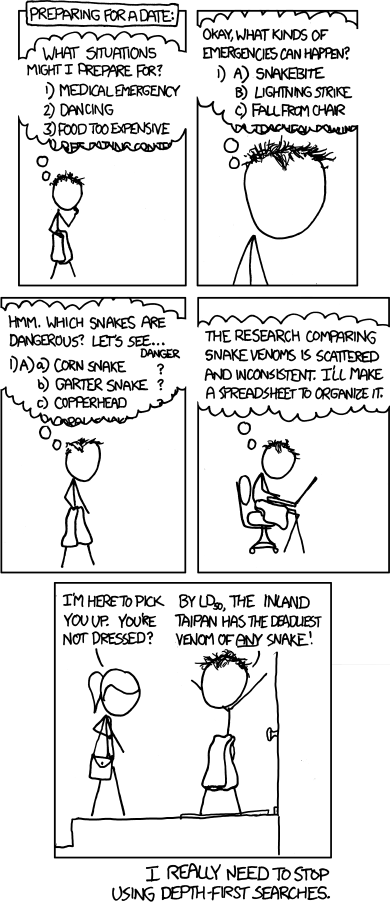
\includegraphics[keepaspectratio,width=0.58\textwidth]{elements/images/dfs_2.png}\par
  \vspace{5pt}
  \tiny{BY-NC 2.5 xkcd.com}
\end{center}
\par
\vspace*{-10pt}
\vfill
\null
\newpage
\tvisa{ATT KRYDDA BRÄNNVIN}
\vspace{10pt}
\setlength{\parindent}{15pt}
När man gör egna kryddningar bör det brännvin 
man använder helst inte vara för starkt om kryddsmaken 
skall komma till sin fulla rätt. Man utgår från okryddat 
brännvin, renat eller vodka.

Oftast går tillverkningen av essens till så att man 
lägger bär eller blommor i en flaska och häller över så 
mycket brännvin att det täcker. Sedan låter man flaskan 
stå i rumstemperatur en vecka och silar därefter bort bär 
eller blommor. Är essensen grumlig ska man låta den stå 
upp till ett halvår. Sedan häller man försiktigt över 
essensen till en annan flaska så att bottensatsen blir kvar.\par
\vspace{10pt}
\noindent\underline{Björkskottens brännvin}\par
\vspace{10pt}
Låter det inte romantiskt? Och björkar har vi ju gott 
om så vi behöver inte vara rädda för att göra någon större 
skada i naturen.

Strax innan björken fått sina första ``musöron'', när 
knopparna fått en liten, liten tipp av grönt, då är den rätta 
tiden att plocka skotten. Stoppa dem i en flaska, häll 
brännvinet över och låt essensen stå och dra i ungefär en 
vecka i rumstemperatur.

Då har ni fått en guldbrun vätska som smakar 
ganska starkt. Blanda ett drygt snapsglas essens med en 
halv flaska brännbin. Ingen kan gissa hur drycken är 
kryddad - men god är den!
\newpage
\noindent\underline{Besk - Malörtsbrännvin}\par
\vspace{10pt}
Besk är en gammal pålitlig snaps där grundkryddan 
är malört. Se bara upp när ni plockar malört så att ni inte 
förväxlar den med den vanliga svinmålan! Malörten har 
silvergrå, lite ludna blad och en hård stam, som är lätt att 
bryta av. Blommorna är små och oansenliga och gula.

Vill man göra ett riktigt fint malörtsbrännvin skall 
man bara använda blommorna. Först ska de hänga och 
torka på sina stjälkar, helst i ett dragigt rum, sedan är det 
lätt att dra av blommorna.

Lägg dem på ett fat, slå över en smula brännvin och 
tänd på. Elden slocknar snart och då stoppas blommorna i 
en flaska som sedan fylls med brännvin. Får stå en vecka, 
varefter essensen silas och lagras.

Det går också att använda både blad och de finare 
stjälkarna till essensen om man så vill.

Många tycker särskilt mycket om att få en ``besk'' 
till julens feta mat. Av gammalt har besken namn om sig 
att hjälpa till med matsmältningen.\par
\setlength{\parindent}{0pt}
\vspace{10pt}
{\footnotesize\textit{Ur boken ``Snapsvisor och brännvinsrecept''.}}

\newpage
\fvisa{KAMELEN PÅ KANELEN}{Om jag vore ett tvåpuckligt djur}
{\footnotesize\textit{Melodi: Old McDonald}}\par
\vspace{10pt}
Om jag vore ett tvåpuckligt djur\\
Eta-eta-nol\\
Kunde jag super i ur och skur\\
Eta-eta nol\\
Fett, fett, fett, bärverfett\\
Bäverfett gör livet lätt\par
\vspace{10pt}
När man går i Kemikums öken\\
Eta-eta-nol\\
Vill man gärna ta till kröken\\
Eta-eta-nol\\
Fett, fett, fett, ...\par
\vspace{10pt}
När jag spriten lagrat upp\\
Eta-eta-nol\\
Klår jag lättans upp en mupp\\
Eta-eta-nol\\
Fett, fett, fett, ...\par
\vspace{10pt}
Nu när nubben slinker ner\\
Eta-eta-nol\\
Jag redan längar efter mer\\
Eta-eta-nol\\
Fett, fett, fett, ...

\newpage
\visa{Livet är härligt}
{\footnotesize\textit{Melodi: Röda kavalleriet}}\par
\vspace{10pt}
int i = 0\\
\revrpt Livet är härligt!\\
Tavaritj, vårt liv är härligt!\\
Vi alla våra små bekymmer glömmer\\
När vi har fått en tår på tanden, skål!\\
Tag dig en vodka!\\
Tavaritj, en liten vodka!\\
Glasen i botten vi tillsammans tömmer!\par
\vspace{10pt}
0: Det kommer mera efter ha-a-and.\\
1: Det kommer mera efter hand, en skål!\\
i++\rpt


\vspace{15pt}
\fvisa{LAPPVISA}{Att vi är lappar det hör ni på sången}
{\footnotesize\textit{Melodi: När jag var liten}}\par
\vspace{10pt}
Att vi är lappar det hör ni på sången.\\
Att vi är fulla det ser ni på gången.\\
Vi drick' brännvin för vi tycker om'en.\\
Det gör så gott när den rinn' uti vommen.\\
\\
Lappmössa med tofs på\\
Fy fan vad det snöar!

\newpage
\visa{Uti vår mage}
{\footnotesize\textit{Melodi: Uti vår hage}}\par
\vspace{10pt}
Uti i vår mage där växa begär,\\
kom hjärtans fröjd.\\
Vill du oss något, så träffas vi där\\
Kom Renat och Aqua Vitae,\\
kom OP och allt vad sprit e'\\
kom ljuva genever,\\
kom hjärtans fröjd.\\
\\
Uti i min mage en längtan mig tär,\\
kom hjärtans fröjd.\\
Där råder en hunger, som ropar så här:\\
Kom kryddsill och kall potatis,\\
kom brännvin och quantum satis,\\
kom allt som kan drickas,\\
kom hjärtans fröjd.\\
\\
Uti mitt hjärta en längtan mig tär,\\
kom hjärtans fröjd.\\
Där råder en hunger som ropar så här:\\
Kom famnande lena armar,\\
kom läppar och sköna barmar,\\
kom fagraste kvinnor,\\
kom hjärtans fröjd.

\newpage
\visa{Samla er go' vänner}
{\footnotesize\textit{Melodi: Sjösalavalsen}}\par
\vspace{10pt}
Samla er go vänner, nu skall vinet begås\\
fatta den i vinbenet, böj den mot skyarna.\\
Ljuvaste av nektar som på bolaget fås\\
dränker oss i vällust och smörjer vårt krås\\
Livet går i vågor, nu kan vi hoppa bock,\\
det där med dagen efter betrakta vi som skrock,\\
i morgon ska vi vakna i skor å hatt å rock å dilla\\
om gullviva, mandelblom, kattfot och blå viol.

\vspace{15pt}
\visa{Tänk om man hade}
{\footnotesize\textit{Melodi: Hej tomtegubbar}}\par
\vspace{10pt}
\revrpt Tänk om jag hade lilla nubben
uppå ett snöre i halsen.\rpt
Jag skulle dra den upp och ner,\\
så att den kändes som många fler.\\
Tänk om jag hade lilla nubben\\
uppå ett snöre i halsen.

\vspace{15pt}
\visa{FINSK SNAPSVISA}
\vspace{10pt}
Korta versionen:\\
Nu!!\par
\vspace{10pt}
Långa versionen:\\
Inte nu men, Nu! (Ei nyt, mutta nyt!)
\newpage
\visa{VI ÄRO SMÅ HUMLOR}
{\footnotesize\textit{Melodi: Här kommer Karl-Alfred Boy}}\par
\vspace{10pt}
Vi äro små humlor vi, bzzz bzzz.\\
vi äro små humlor vi, bzzz bzzz.\\
vi äro små humlor som,\\
tar oss en geting.\\
vi äro små humlor vi, bzzz bzzz.\par
\vspace{10pt}
Vi äro små fiskar vi, blubb blubb.\\
vi äro små fiskar vi, blubb blubb.\\
vi äro små fiskar,\\
som tar oss en kallsup.\\
vi äro små fiskar vi, blubb blubb.\par
\vspace{10pt}
Vi äro små änglar vi, flax flax.\\
vi äro små änglar vi, flax flax.\\
vä äro små änglar,\\
som tar oss en DJÄVEL.\\
vi äro små änglar vi, flax flax.

\vspace{15pt}
\fvisa{Domkyrkan}{Domkyrkan stilla står}
{\footnotesize\textit{Melodi: Karl-Alfred Boy}}\par
\vspace{10pt}
Domkyrkan stilla står.\\
Har gjort så i många år.\\
Så synes den gunga,\\
när vi slutat sjunga,\\
beror det å nåbben vår,\\
gutår!

\newpage
\visa{HANDEN ÄR VILLIG}
{\footnotesize\textit{Melodi: When I'm sixty-four}}
\vspace{10pt}
Handen är villig, glaset är höjt,\\
armen har man böjt.\\
Tittar man sig kring och ser högtidlig ut,\\
minns att två man tagit förut.\\
Bägge besjungits och vägen röjt,\\
för en tredje vers.\\
Helan oss väckte.\\
Halvan ej räckte.\\
Nu tar vi en ters!

\vspace{15pt}
\fvisa{CYKELHANDLARENS VISA}{Hoj}
\vspace{10pt}
Hoj!

\vspace{15pt}
\visa{DENNA THAFT}
{\footnotesize\textit{Melodi: Helan går}}\\
\\
Denna thaft,\\
är den bätha thaft thythemet haft.\\
Denna thaft,\\
är den bätha thaft dom haft.\\
Och den thom inte har nån kraft\\
han dricka thkall av denna thaft.\\
Denna thaft,\\
till landth, till sjöth, till havth.

\newpage
\visa{LINGONRÖDA NÄSOR}
{\footnotesize\textit{Melodi: Flickorna i Småland}}\par
\vspace{10pt}
Med lingonröda näsor\\
och med bullranda bas\\
och skinande som solen\\
uppå våra små kalas,\\
vi sjunga och vi tralla\\
när när vi höja våra glas\\
men vad är det som gör\\
att vi nu komma i extas?\\
Det är en stänk av livets vatten\\
det är helan lilla vän,\\
det är litrarna som staten\\
inte lagt beslag på än.\\
Det blir halva tersen, qvarten\\
och en grogg vi dricka se'n,\\
och till morgonen vi spart\\
den lilla återställaren.

\vspace{15pt}
\fvisa{Helan gick i vänstra foten}{Helan gick i vänstra foten}
{\footnotesize\textit{Melodi: Amanda Lundbom}}\par
\vspace{10pt}
Helan gick i vänstra foten, bomfaderi och faderaderalla.\\
Gudskelov så vet jag boten, bomfaderi faderallanlej.\\
Halvan ställer saken rätt, bomfaderi faderallanlej.\\
Hugg i!\\
På nubbar blir man aldrig mätt, bomfaderi faderallanlej.
\newpage
\fvisa{MINNE}{Minne"! Jag har tappat mitt minne}
{\footnotesize\textit{Melodi: Memory ur musikalen Cats}}\\
\\
Minne! Jag har tappat mitt minne\\
är jag svensk eller finne?\\
Kommer inte ihåg\\
\\
Inne! Är jag ute eller inne?\\
Jag har luckor i minne\\
såna där små alkohol.\\
\\
Men besinne, man tätar det med brännvin \\
som man får fastän minnet \\
och helan den går.\\
\\
{\footnotesize\textit{Text: Bosse Österberg}}

\vspace{15pt}
\visa{BE- BE- VITAMIN}
{\footnotesize\textit{Melodi: Bä bä vita lamm}}\\
\\
Be-Be- vitamin, finns i brännevin.\\
Mången kalori, simmar däruti.\\
Helgdagssup åt far,\\
och söndagskrök åt mor\\
samt tre små huttar\\
åt lille lille bror.

\newpage
\fvisa{Segersnapsvisa}{När vi satt oss att äta sill}
{\footnotesize\textit{Melodi: Gånglåt från Äppelbo}}\par
\vspace{10pt}
När vi satt oss att äta sill\\
ska vi ta den snaps som hörer därtill\\
och en till och en till för till varje liten sill\\
får vi snapsa så mycket vi vill!\\
\\
Men om nu ingen sill vi har\\
så betyder det ej att på brännvin vi spar\\
vi har ännu kvar så det räcker några dar\\
så ett stadigt grepp om glaset vi tar.\\
\\
Här i vänners lag stäm nu upp och sjung\\
och strunta i om våran morgondag blir tung\\
göra livet till fest det är kodarens mål\\
så vi höjer våra glas med ett vrål: SKÅL!
\par
\vspace{10pt}
{\footnotesize\textit{M-sektionen LTH, sångarstriden 1991}}

\vspace{15pt}
\visa{Fjompe tompe törstig}
{\footnotesize\textit{Melodi: Imse vime spindel}}
Fjompe tompe törstig sitter i en bar\\
Vickar på stolen o i golvet far\\
Strax nån fyller på hans glas o sen\\
Fjompe tompe törstig klättrar upp igen.

\newpage
\visa{Vi skålar för våra vänner}
{\footnotesize\textit{Melodi: Flickan går i ringen}}\par
\vspace{10pt}
Vi skålar för våra vänner,\\
och dom som vi känner,\\
och dom som vi inte känner,\\
dom skiter vi i!\par
\vspace{10pt}
Vi skiter i våra vänner,\\
och dom som vi känner,\\
och dom som vi inte känner,\\
dom skålar vi för!

\vspace{15pt}
\visa{EN GÅNG I MÅNAN}
{\footnotesize\textit{Melodi: Mors lilla Olle}}\\
\\
En gång i månan är månen full,\\
men aldrig jag sett honom ramla omkull.\\
Stum av beundran hur mycket han tål,\\
höjer jag glaset och säger nu skål!\\
\\
Höjer nu glasen och dricker ur.\\
Nu kära bröder, står helan (halvan) i tur.\\
Nubben den giver oss ny energi,\\
säkert den minskar vårt livs entropi.

\newpage
\visa{Första snapsen}
{\footnotesize\textit{Melodi: Räven raskar över isen}}\par
\vspace{10pt}
Första snapsen heter göken.\\
Första snapsen heter göken.\\
Får jag lov, ja far jag lov\\
att byta byxor med fröken?\par
\vspace{10pt}
Andra snapsen den var värre,\\
andra snapsen den var värre.\\
Får jag lov, får jag lov\\
att byta byxor med min herre\par
\vspace{10pt}
Mina byxor är himmelsblå\\
men med dina är det dock si och så.\\
Får jag lov, far jag lov,\\
att byta byxor med göken.

\vspace{15pt}
\visa{FÖRSTA SUPEN}
{\footnotesize\textit{Melodi: Oh, Susanna}}
\vspace{10pt}
Första supen har nu runnit ner,
men se magen vill ha mer.
Om vi inte genast Halvan tar
höres magens kommentar:

O, besinna, den saken är ju klar;
både magsår, tarmvred och kolik
dunstar bort med lite sprit.

\newpage
\fvisa{Glädjetåren}{Helan, sköna Helan"!}
{\footnotesize\textit{Melodi: Familjen Flinta}}\par
\vspace{10pt}
Helan, sköna Helan!\\
Ljuva droppar i en glädjetår!\par
\vspace{10pt}
Helan, fegt att dela'n!\\
Den ger styrka och du bättre mår!\par
\vspace{10pt}
Men spriten, dödar långsamt har man spått!\\
Tur de', för vi har knappast brått!\par
\vspace{10pt}
Livet, det är givet.\\
Det skall levas fyllt av glädje,\\
ni måste medge:\\
Bäst är en glädjetår!

\vspace{15pt}
\fvisa{JUNGFRU JUNGFRU}{}
{\footnotesize\textit{Melodi: Karusellen}}\par
\vspace{10pt}
Jungfru, jungfru, jungfru, jungfru kär\\
här har'n putellen\\
i tomma glasen häll'en\\
tio för de stora, fem för de små\\
skynda på, skynda på, om en stund skall helan gå.\par
\vspace{10pt}
För ha, ha, ha, det ska smaka ju bra\\
det dammar ju i strupen vareviga da'\\
För ha, ha, ha, nu helan vi ta\\
båd' Andersson och Pettersson och Lundström och jag.

\newpage
\visa{Vårsupar friska}
{\footnotesize\textit{Melodi: Vårvindar friska}}\par
\vspace{10pt}
Vårvindar friska, leka och viska:\\
tag dig en sup i majsolens glans!\\
Strömkarlen spelar, sorgen fördelar\\
brännvinet med en viss elegans!\\
Andas blott djupt, ty helan nu går,\\
och efter helan halvan du får.\\
Skål mina vänner, våren vi känner,\\
låtom oss tappa måtta och sans! \\
\\
Vårvindar friska borde snart viska\\
stunden är kommen att vara glad.\\
Spetsa ditt öra; nog kan du höra\\
våren är kommen, fast den är svag.\\
Klunkom av hjärtat, klaga ej mer\\
klingen med glasen; gör som vi ber.\\
Herrar till höger, damer till vänster.\\
Skål för en vår som kommer. - Gutår!

\vspace{15pt}
\fvisa{Invers Aptit}{Nu fyllas många magar små}
{\footnotesize\textit{Melodi: Nu tändas tusen juleljus}}\par
\vspace{10pt}
Nu fyllas många magar små av iskall renad sprit.\\
Men många kastar åter opp, det är invers aptit.

\newpage
\fvisa{Sista Snapsen}{Festen den har varit}
{\footnotesize\textit{Melodi: Flickan i Havanna}}\par
\vspace{10pt}
Festen den har varit\\
mycket glad och lite våt\\
nu den snart är över\\
- skiljas det blir svårt.\\
Vi har druckit mången snaps\\
nu sägs det vara dags\\
sista lilla nubben ta\\
alla vill väl ha?\\
\\
Sillen har vi ätit\\
opp för flera timmar sen\\
men att snapsen drickes\\
än har vi på känn.\\
Låt oss all skåla nu\\
sista droppen den får du,\\
men när nästa gång vi ses\\
mera dricka ges.

\vspace{15pt}
\visa{MAGEN BRUMMAR}
{\footnotesize\textit{Melodi: Broder Jakob}}\par
\vspace{10pt}
Magen brummar, jag försummar,\\
hälla dit mer sprit.\\
Nu så ska vi dricka, så att vi får hicka,\\
mera sprit, akvavit.

\newpage
\fvisa{Getingen}{Och så kommer det en geting}
{\footnotesize\textit{Melodi: Jazzgossen}}\par
\vspace{10pt}
Och så kommer det en geting\\
genom luften som ett reaplan.\\
Och ger dig en liten snyting\\
mitt under röda kran.\\
Och så åker han i magen\\
med ett litet plask,\\
litet plask, litet plask.\\
Och så blir man lite dragen,\\
men pigg och rask,\\
pigg och rask, pigg och rask.

\newpage
\null
\vfill
\vspace*{-10pt}
\index{Ã1337: Part 1@1337: Part 1}
\begin{center}
  \label{13371}
  \tiny{1337: Part 1}\par
  \vspace{5pt}
  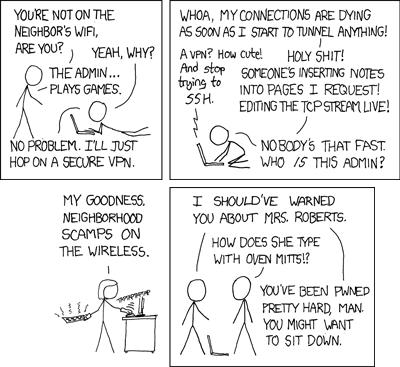
\includegraphics[keepaspectratio,width=0.8\textwidth]{elements/images/1337_part_1_1.png}\\
  \textline[t]{}{\tiny{BY-NC 2.5 xkcd.com}}{\tiny{\textit{forts. $\rightarrow$ s.\pageref{13372}}}}\par
\end{center}\par
\vfill
\null
\chapterpageimage{Ölvisor}{Ölvisor}{elements/ol.jpg}
\tvisa{LITE OM ÖL}
\vspace{10pt}
\hspace{10pt}Öl, alkoholdryck framställd av mältad säd (oftast korn), humle, vatten
och jäst.\par
\vspace{10pt}
\hspace{10pt} Konsten att brygga öl utvecklades san under yngre
stenåldern. I Mesopotamien finns uppgifter om flera olika sorters öl
redan från ca 3000 f.Kr., och i Egypten framställdes öl åtminstone
från Gamla rikets tid (ca 2700 – 2270 f.Kr.).\par
\hspace{10pt} I Norden har påträffats gravkärl från bronsåldern
(ca 1800 – 500 f.Kr.) med rester av intorkat öl.\par
\hspace{10pt} Metoderna har växlat och kan variera än
idag. Man utgår dock alltid från en sädesråvara som mältas, för att
dess stärkelse under den följande vörtbryggningen skall kunna lösas i
vatten och omvandlas till socker, vilket i sin tur jäses till alkohol,
kolsyra och smakämnen. Det så erhållna ölet smaksätts normalt med
någon krydda, numera praktiskt taget alltid humle.\par
\hspace{10pt}Öl med en alkoholhalt över 0,5 volymprocent beskattas efter
alkoholhalten. Skatten är 1,66 krona per volymprocent alkohol och
liter öl. Ett särskilt undantag görs för öl med en alkoholhalt under
2,8 volymprocent, där skatten är 0 kronor.

\newpage
\fvisa{UD EFTER ØL}{Der var en skikkelig bondeman}
\vspace{10pt}
\revrpt Der var en skikkelig bondeman
han skulde gaa ud efter øl. \rpt
Han skulle gaa ud efter øl,
han skulle gaa ud efter øl,
efter øl, efter hoppsan sa tra la la la,
han skulle gaa ud efter øl.

\revrpt Til konen kom der en ung student
mens manden var ud efter øl. \rpt
Mens manden var ud efter øl, ...

\revrpt Han kysste henne paa rosenmund
og klapped henne paa kind \rpt
Mens manden var ud efter øl...

\revrpt Men manden stod bag ved døren og så
hvordan det hele gik til. \rpt
For de trod han var ud efter øl, ...

\revrpt Han skød studenten och kæringen med,
og så gik han ud efter øl. \rpt
Og så gik han ud efter øl, ...

\revrpt Moralen er: Tag din kone med,
hver gang du skal ud efter øl. \rpt
Hvar gang du skal ud efter øl, ...
\vspace{10pt}
{\footnotesize\textit{Efter öl kan även sjungas n gånger, där en är versens nummer.\\
Detta enligt F KTH:s sångbok.}}

\newpage
\fvisa{LAMBO}{Sätt nu glaset till din mun"!}
\vspace{10pt}
Sätt nu glaset till din mun!\\
Tjofaderitan, lambo!\\
Och drick ur din fylle-, fyllehund!\\
Tjofaderitan, lambo!\\
Se hur dropparna i glaset\\
rinner ner i fylleaset.\\
Lambo hej, lambo hej, \\
tjofaderitan lambo!\\
\\
\textbf{Jag nu glaset druckit har!}\\
Tjofaderitan lambo\\
\textbf{Ej en droppe finnes kvar!}\\
Tjofaderitan lambo.\\
\textbf{Som bevis jag nu vill vända\\
glaset på dess ``rätta'' ända.}\\
Lambo hej, lambo hej\\
tjofaderitan lambo.\\
\\
Ja, han kunde konsten,\\
han var en äkta fylle-, fyllehund.\\
Så låt oss gå till nästa man\\
och se vad han förmår\\
\\
(\textit{En liten variant})\\
\textbf{Som bevis jag nu vill föra\\
glaset till min grannes öra}

\newpage
\fvisa{ÖLVISAN}{Dricka pilsner varje da'}
{\footnotesize\textit{Melodi: SJ, SJ gamle vän}}
\vspace{10pt}
\\
Dricka pilsner varje da'\\
de é kul å de é bra\\
Ja, det borde alla ha,\\
pilsner varje da'.\\
\\
Öl det slinker ner så lätt\\
lättare än fläskkotlett\\
Å när en har slunkit ner\\
så måste man ha fler\\
\\
Efter sex, sju flaskor till\\
blir det svårt att sitta still\\
Å vid cirka trettitvå\\
blir det svårt att gå\\
\\
Öl de é ju faktiskt mat\\
öl på burk å öl på fat\\
Måste fyllas på i ett\\
för annars går det snett\\
\\
Ingen har väl illa mått\\
utav öl som är så gott.\\
Den som ändå detta gjort\\
har druckit det för fort.\\
\\
Så korka upp din öl å drick\\
så blir du en festlig prick\\
Korka upp å drick min vän\\
och rapa högljutt sen'.

\vspace*{-10pt}
\newpage
\fvisa{OH, LJUVA ÖL}{Jag har nu fått en och annan öl}
{\footnotesize\textit{Melodi: Kung Louis sång}}\\
\\
Jag har nu fått en och annan öl,\\
som jag genast druckit har.\\
Ja, jag har druckit mycket jag.\\
Jag ingen droppe spar.\\
För nu vill jag bara festa,\\
tills jag far ikull.\\
Jag vill ej längre nykter va.\\
Jag vill bara vara full.\\
\\
Oh, ljuva öl, vad jag är glad åt öl.\\
För jag vill dricka den, och en till, öl.\\
Det vill jag nu, ett djur som jag,\\
det lär sig bra bli en fyllehund.\\
\\
Försök inte hindra mig gosse,\\
för nu så är det fest.\\
Och då man drycker dricka ska,\\
som gjorda är på jäst.\\
Så ge mig nu inget annat,\\
att hälla i mitt glas.\\
för nu så ska jag dricka ur,\\
och bli full som ett as.

\newpage
\fvisa{MELLANÖLSKVARTETT}{Säg har ni känt nåt vått som är gott}
{\footnotesize\textit{Melodi: Nu grönskar det.}}
\vspace{10pt}
Säg har ni känt nåt vått som är gott\\
som det ni nu har fått.\\
Nej, här har ni ett eau de vie\\
med humle och dumle i.\\
Den klunken visste var den tog\\
mmmmmmmmmmmmmmm.\\
Det är det bästa som jag känt\\
med tre komma sex procent.\\
\\
Den finns på fik, i var butik\\
är lagrad, men ej antik.\\
Den ställes fram med stor reklam\\
för folk av frejdad stam.\\
Det krävs ej legitimation\\
mmmmmmmmmmmmm.\\
Nej, frihetsklockan högljutt slår,\\
om man fyllt arton år.\\
\vspace{10pt}
{\footnotesize\textit{Ur Chalmerspexet Sven Duva}}

\vspace{15pt}
\visa{ÖLFLASKOR SMÅ}
{\footnotesize\textit{Melodi: Mors lilla Olle}}\par
\vspace{10pt}
Ölflaskor små uti backarna stå,\\
stiger i pris men vi säger som så:\\
Priset på brännvin och öl kan ej nå\\
upp till sitt verkliga värde ändå.

\newpage
\fvisa{STREJK PÅ PRIPPS}{I natt jag drömde något som}
{\footnotesize\textit{Melodi: I natt jag drömde}}\par
\vspace{10pt}
I natt jag drömde något som,\\
jag aldrig drömt förut.\\
Jag drömde det var strejk på Pripps\\
och alla ölen var slut.\\
Jag drömde om en jättesal\\
där ölen stod på rad.\\
Jag drack så där ett tjugotal\\
och reste mig och sa;\par
\vspace{10pt}
Armen i vinkel\\
blicken i skyn\\
så var det menat\\
whisky och renat\\
vårt mål alkohol!\\
För dem som tålt! - SKÅL

\vspace{15pt}
\visa{MIN PILSNER}
{\footnotesize\textit{Melodi: My Bonnie}}
\vspace{10pt}
Min pilsner skall svalka min tunga.\\
Min pilsner skall duscha min gom.\\
Min pilsner skall få mig att sjunga,\\
om jag ser att flaskan är tom:\\
Pilsner! Pilsner!\\
Hämta en pilsner till mig, till mig.\\
Pilsner! Pilsner!\\
Hämta en pilsner till mig!

\newpage
\fvisa{ØL, ØL HERLIGE ØL}{Øl, øl herlige øl,}
{\footnotesize\textit{Melodi: Trink, trnik...}}\par
\vspace{10pt}
Øl, øl herlige øl,\\
gult som det gyldneste rav.\\
Øl, øl herlige øl,\\
du er min lønligste krav.\\
\revrpt Dug perler kruset,\\
oh, mø vaer ej grum,\\
kys mig, du dejlige skum.\rpt

\vspace{15pt}
\fvisa{ÖL, ÖL}{}
{\footnotesize\textit{Melodi: Ritsch, ratsch}}
\vspace{10pt}
Öl, öl fillibombombom, fillibombombom, fillibombombom.\\
Öl, öl fillibombombom, fillibombombom, fillibom.\\
Vi har ju både Heineken och Nordic Wölf,\\
Tuborg Guld och lilla Preppens Blå.\\
Det blir för trist med sodavatten,\\
sodavatten, sodavatten,\\
det blir för trist med sodavatten,\\
ge mig lite öl!

\vspace{15pt}
\fvisa{ÖL, ÖL}{}
{\footnotesize\textit{Melodi: Row, row, row your boat}}
\vspace{10pt}
Öl, öl, öl i glas, eller i butelj.\\
Skummande, skummande,\\
skummande, skummande.\\
Ta en klunk och svälj!

\newpage
%% Ska ligga tillsammand med skummande cider
\fvisa{SKUMMANDE ÖL}{När skummande öl har hällts upp i var glas}
{\footnotesize\textit{Melodi: The Wild Rover}}\par
\vspace{10pt}
När skummande öl har hällts upp i var glas\\
Leenden tänds för nu vankas kalas\\
Du ser på din granne och glädjen får svar\\
Det är dukat för båda, ni har en öl var\par
\vspace{10pt}
\revrpt För av alla drycker (- - - -)\\
Som vi har på vår jord\\
Är det alltid en öl\\
Jag vill ha på mitt bord\rpt\par
\vspace{10pt}
Med smak utav korn ifrån böljande fält\\
Ger det livslust i festsalar, pubar och tält\\
Ett gyllene skimmer som sol över hav\\
Ett framgångsrecept ifrån vagga till grav\par
\vspace{10pt}
{\footnotesize\textit{Text tillägnad Uplands av: Hörn, Dannfors, Ingo och Elias}}

\vspace{15pt}
\visa{LAPIN KULTA}
{\footnotesize\textit{Melodi: Broder Jakob}}\\
\\
Lapin Kulta, Lapin Kulta\\
Karjala, Karjala\\
Aura sekä Olvi, Aura sekä Olvi\\
Koff, Koff, Koff\\
Koff, Koff, Koff

\newpage
%% Ska ligga tillsammand med skummande öl
\fvisa{SKUMMANDE CIDER}{När skummande cider har hällts upp i var glas}
{\footnotesize\textit{Melodi: The Wild Rover}}\par
\vspace{10pt}
När skummande cider har hällts upp i var glas\\
Leenden tänds för nu vankas kalas\\
Du ser på din granne och glädjen får svar\\
Det är dukat för båda, ni har en cider var\par
\vspace{10pt}
\revrpt För av alla drycker (- - - -)\\
Som vi har på vår jord\\
Är det alltid en cider\\
Jag vill ha på mitt bord\rpt\par
\vspace{10pt}
Med saftiga frukter från gungande träd\\
Ger det smaker långt bättre än humle och säd\\
Ett gyllene skimmer som sol över hav\\
Ett framgångsrecept ifrån vagga till grav\par
\vspace{10pt}
{\footnotesize\textit{Text tillägnad Uplands av: Hörn, Dannfors, Ingo \& Elias}}

\vspace{15pt}
\visa{VAR NÖJD MED ÖLEN}
{\footnotesize\textit{Melodi: Var nöjd med allt vad livet ger.}}
\vspace{10pt}
Var nöjd med allt som ölen ger\\
och även om du dubbelt ser.\\
Glöm bort bekymmer sorger och besvär.\\
Var glad och nöjd för vet du vad\\
en folköl gör ju ingen glad.\\
Var nöjd med ölen som vi dricker här.

\newpage
\fvisa{DRÖMMEN OM ÖLEN}{Nu så har vi fest}
{\footnotesize\textit{Melodi: Drömmen om Elin}}
\vspace{10pt}
Nu så har vi fest.\\
Det går sång ur alla strupar.\\
Ölen är vår gäst,\\
ibland sill och supar.\\
Tredje klass ger mest,\\
och om du blir trött och stupar:\\
Drömmen om ölen låter dig festa igen!\\
\\
På vårt ölkalas,\\
där finns inga fat och koppar.\\
Stora sejdelglas\\
helt servisen toppar.\\
När den sista tas,\\
och du själv går hem och knoppar:\\
Drömmen om ölen låter dig festa igen!\\
\vspace{10pt}
{\footnotesize\textit{Ur Linköpingsspexet ``da Gama och havet'',1988}}

\vspace{15pt}
\fvisa{NÄR JAG KISSAR ÖVERALLT}{På gator som trampats av Ask och von Platen}
{\footnotesize\textit{Melodi: }}
\vspace{10pt}
På gator som trampas av Ask och von Platen.\\
På stenar som blickat på Broman, Piraten.\\
På Lundagårds träd som har skuggat Tegnér.\\
På allt har jag kissat och lustfyllt blött ner.
\vspace{10pt}
{\footnotesize\textit{Lundakarnevalen 1986}}

\newpage
\visa{JU MER VI DRICKER PILSNER}
{\footnotesize\textit{Melodi: Ju mer vi är tillsammans}}
\vspace{10pt}
Ju mer vi dricker pilsner\\
Pilsner, pilsner.\\
Ju mer vi dricker pilsner,\\
ju gladare vi bli.\\
\\
Ta en Pripps,\\
sen två Pripps.\\
Sen tar vi \\
en back Pripps.\\
\\
Ju mer vi dricker pilsner,\\
ju gladare vi bli.

\vspace{15pt}
\fvisa{HÄSTHANDLAR'N}{Ur ett glas vid bordets slut}
{\footnotesize\textit{Melodi: I ett hus vid skogens slut}}
\vspace{10pt}
Ur ett glas vid bordets slut\\
liten starköl rinner ut.\\
Lennart stirrar på sitt stop\\
bryter nog ihop.\\
Nej, han vaknar ur sin nöd\\
cyklar hem till Veberöd\\
pantsätter sin systers föl\\
tusen spänn till öl.\\
\vspace{10pt}
{\footnotesize\textit{Ur sångboken från Lunda karnevalen 1994.}}

\newpage
\fvisa{MER ÖL}{Jag är en lugn person med takt och ton}
{\footnotesize\textit{Melodi: Mer jul}}
\vspace{10pt}
Jag är en lugn person med takt och ton\\
måttfull och balanserad.\\
Jag är tyst och still och det skall mycket till\\
innan jag blir exalterad.\\
\\
Men jag har en last som håller mig fast\\
i ett järngrepp varje fredag.\\
När veckan är slut, ger jag mig ut\\
och flyr från varda’ns leda.\\
\\
\revrpt Jag vill ha mer öl, så ge mig mer öl. \rpt\\
Tusen bubblor som glimmar\\
flaskor så långt man ser\\
skum i glaset som simmar\\
jag vill ha mer.\\
\\
Med svalget torrt jag drömmer mig bort,\\
en kväll när svetten lackar.\\
Så ge mig lagom kallt, lagom malt\\
i lagom stora backar.\\
\\
Så ge mig Kaltenberg och Falkenberg\\
och Tuborg det som finnes.\\
Och ge mig sen en Heineken\\
en Spendrups och en Guinness.\\
\\
Jag vill ha mer öl...\\
\\
Ett jätteglas Stella Artois,\\
i Carlsberg vill jag plaska.\\
Jag tar en till och en snabb Dab\\
innan du hinner säga flaska.\\
\\
Ge mig en Pripps och en påse chips,\\
annars får du en blåtira.\\
En jättepråm med Kaiserdom\\
en bärs, en pils, en bira.\\
\\
Jag vill ha mer öl...

\vspace{15pt}
\fvisa{VI ÄLSKAR ÖL}{Täckt av silver sejdeln full}
{\footnotesize\textit{Melodi: Ser du stjärnan i det blå?}}
\vspace{10pt}
Täckt av silver sejdeln full\\
gnistrar mot oss med sitt guld\\
humle, malt, är livets salt, vi älskar öl.\\
\\
Källarsval så bärs den in\\
för att glädja gommen din\\
släcka törsten, stärka rösten, till dess lov.\\
\\
Knubbig blir du, men so what\\
gott och roligt har du fått\\
extra turen, rensat njuren, öl är gott.

\newpage
\visa{Johan går tunga fjät}
{\footnotesize\textit{Melodi: Natten går tunga fjät}}\par
\vspace{10pt}
Johan går tunga fjät\\
runt Per och Mitra\\
Han inte alls förlät\\
tunghäftans pina\\
Men ölen blir hans vän\\
kostar nog tretti spänn\\
Lossar tungans band kring flabben\\
Poppis blir grabben

\vspace{15pt}
\fvisa{PILSNERVISAN}{Säg var finns det pilsner}
{\footnotesize\textit{Melodi: Down by the riverside}}\par
\vspace{10pt}
Säg var finns det pilsner.\\
I speceriaffärn\\
I speceriaffärn\\
I speceriaffärn\\
Säg var finns det pilsner.\\
I speceriaffärn, i speceriaffärn.\\
Där har dom Lyckholms och klass 1\\
och prippes blåa etikett.\\
Men bara klass 2 och 1\\
Och om du ville ha klass 3\\
så gå till bolaget breve.\\
Ja de' va en bra idé.

\newpage
\visa{EN PILSNERDRICKARE}
{\footnotesize\textit{Melodi: En sockerbagare}}\par
\vspace{10pt}
En pilsnerdrickare här bor i staden,\\
han dricker pilsner mest hela dagen,\\
han dricker gröna, han dricker blå,\\
han dricker några med renat på.\par
\vspace{10pt}
Och i hans fönster hänga tomma glasen,\\
och alla burkarna ifrån kalasen,\\
och är han nykter så kan han gå\\
ner till butiken och fylla på.

\vspace{15pt}
\visa{ÖL AV DIG}
{\footnotesize\textit{Melodi: All of me}}\par
\vspace{10pt}
Öl av dig.\\
Jag vill ha öl av dig.\\
Skicka hit några kalla pilsner.\\
Kärlek nej, jag vill ej ha det.\\
Gifta mej, de får nog va' det.\\
Öl av dig.\\
Jag vill ha öl av dig.\\
Kärlek nej, inga relationer,\\
vill du ha mig\\
så säg inte nej.\\
När jag ber om öl av dig.\par
\vspace{10pt}
{\footnotesize\textit{Ur sångboken från Lunda karnevalen 1990.}}

\newpage
\fvisa{ODE TILL ÖLET}{Tu tu tu Tuborg}
{\footnotesize\textit{Melodi: Trampa på gasen}}
\vspace{10pt}

Tu tu tu Tuborg\\
och ca ca ca Carlsberg\\
det är den bästa\\
$pi$ $pi$ $pi$ pilsnern som jag vet.\\
\\
Tu tu tu Carlsberg\\
och ca ca ca Tuborg\\
det är det bästa\\
$pi$ $pi$ $pi$ ölet som jag vet.\\
\\
Tu tu tu Ölberg\\
och ca ca ca Pilsborg\\
det är den bästa\\
$pi$ $pi$ $pi$ biran som jag vet.\\
\\
Tu ca $pi$ Ölsner\\
och $pi$ tu ca bira\\
det är den bästa\\
ca $pi$ tu lering som jag gjort!

\vspace{15pt}
\fvisa{TUBORG:s KAMPVISA}{Kommer der icke snært en Tuborg til meg}
{\footnotesize\textit{Melodi: Kan man tro...}}
\vspace{10pt}
Kommer der icke snært en Tuborg til meg,\\
Tuborg til meg, Tuborg til meg.\\
Kommer der icke snært en Tuborg til meg.\\
Röd eller grön til meg.

\newpage
\fvisa{ÖL-KANON}{Drick, drick, drick din öl}
{\footnotesize\textit{Melodi: Row, row, row your boat}}\\
\\
Drick, drick, drick din öl\\
låt den rinna ner.\\
Kan du sen kraxa\\
"en laxask med slasktratt”\\
så får du dricka fler.

\vspace{15pt}
\fvisa{I GODA VÄNNERS LAG}{Jag dricker öl när jag ser dig}
{\footnotesize\textit{Melodi: Israelism}}
\vspace{10pt}
Jag dricker öl när jag ser dig.
Jag dricker öl när jag ser dig.
Jag dricker öl när jag ser dig.
Jag dricker öl för att stå ut med att se dig!
\vspace{10pt}
{\footnotesize\textit{Lundakernevalen 1998}}

\vspace{15pt}
\fvisa{GULD!}{OS-guld, EM-guld, VM-guld.}
{\footnotesize\textit{Melodi: Det vanliga skrålet som brukar höras på segerfesterna}}\par
\vspace{10pt}
OS-guld, EM-guld, VM-guld.\\
Tuborg guld, Carlsberg guld, Norrlands guld.\\
OS-guld, EM-guld, VM-guld.\\
Tuborg guld - STUDIESKULD!\par
\vspace{10pt}
{\footnotesize\textit{Ur sångboken från Lunda Karnevalen 1994.}}

\chapterpageimage{Vinvisor}{Vinvisor}{elements/vin.jpg}
\tvisa{Glögghistoria}
\vspace{10pt}
\noindent\hspace*{10pt}Vi har druckit varm, söt julglögg av vin och kryddor sedan slutet av
1800-talet. Däremot har vi efter utländskt mönster värmt oss med
glödgat vin sedan 1600-talet. Medan seden att krydda vin säkerligen är
lika gammal som vinet självt. Antagligen började det med att dölja
dålig smak på vinet, men så småningom blev det också ett sätt att
skryta med sina dyra kryddor.\par
\noindent\hspace*{10pt}Den närmaste föregångaren till julglögg är annars den franska drucken blûlot. Den görs av cognac som värms upp i en gryta. Sedan täner man elden på spriten och öser den över en sockertopp, placerad på ett galler över grytan.\par
\noindent\hspace*{10pt}Färdiggjord glögg på flaska kom strax efter sekelskiftet. De flesta privata vinhandlare höll med egna varianter. Alla med fantasifulla etiketter.\par
\vspace{10pt}
{\footnotesize\textit{Ur Systembolagets tidning ``Julnytt - om glögg och julöl 1995''}}

\newpage
\fvisa{GLÖGGVISA}{Vi ser det snöar}
{\footnotesize\textit{Melodi: Vi ser det snöar}}\par
\vspace{10pt}
Vi ser det snöar,\\
vi ser det snöar,\\
och glöggen vi tar.\\
Vi ser det snöar,\\
vi ser det snöar,\\
varmt i magen hurra!\\
Nu tar vi russinen fram\\
att krydda den med.\\
Sedan magen den får,\\
Och hej vad den mår.

\vspace{15pt}
\fvisa{UNDULATEN}{Jag är en liten undulat}
{\footnotesize\textit{Melodi: Med en enkel tulpan}}\\
\\
Jag är en liten undulat\\
som får så dåligt med mat\\
för dom jag bor hos\\
ja dom jag bor hos\\
dom är så snåla.\\
Jag får ju fisk varenda dag\\
men det vill jag inte ha\\
jag vill ha rödvin\\
jag vill ha rödvin och gorgonzola

\newpage
\fvisa{SOLSKEN I BLICK}{Sjungom så glada till glasens klang}\\
{\footnotesize\textit{Melodi: Mors lilla Olle}}\\
\\
Sjungom så glada till glasens klang\\
vinet det har både heder och rang\\
Alla så får vi på ett ögonblick\\
rosor på kinden och solsken i blick.\\
\\
Gudarnas gåva. O, vilken fröjd.\\
Dofterna stiga mot himlens höjd.\\
Noak planterade vin och han fick\\
rosor på kinden och solsken i blick.\\
\\
Trivsamt och festligt det ska det va'\\
vinet gör människan vänlig och glad\\
vinet ger färg åt den blekaste prick\\
rosor på kinden och solsken i blick.\\
\\
Bröder och systrar nu höj ditt glas.\\
Vinet förljuvar vårt glada kalas.\\
Drick ur ditt glas och du får på ett kick\\
rosor på kinden och solsken i blick.\\
\\
Låtom oss glädjas och kasta loss.\\
Festföremålet skall säga om oss:\\
Gästerna hade, då hemåt de gick\\
rosor på kinden och solsken i blick.

\newpage
\fvisa{FRANSK VINVISA}{Feta fransyskor som svettas om fötterna}
{\footnotesize\textit{Melodi: Schuberts militärmarsch (Tomtarnas vaktparad.)}}\par
\vspace{10pt}
Feta fransyskor som svettas om fötterna,\\
de trampa druvor som sedan ska jäsa till vin.\\
Transpirationen viktig é,\\
ty den ger fin bouquet.\\
Vårtor och svampar följer mé\\
men vad gör väl dé?\par
\vspace{10pt}
För vi vill ha vin, vill ha vin, vill ha mera vin\\
även om följderna bli att vi må lida pin\par
\begin{tabular}{@{}m{0.05\linewidth}p{0.7\linewidth}@{}}
  \scalebox{1.5}{\Female} & Flaskan och glaset gått i sin\\
  \scalebox{1.5}{\Male} & Hit med vin, mera vin\\
  \scalebox{1.5}{\Female} & Tror ni att vi är fyllesvin\\
\end{tabular}\par
(\textit{skrik}) Ja, fast större!\par
\vspace{10pt}
{\footnotesize\textit{Text: Helène Derand\\Sångarstriden 1985 av
    K-LTH}}

\vspace{15pt}
\fvisa{GLÖGGVISAN}{Ack, glöggen den står på bordet}
{\footnotesize\textit{Melodi: Flickan hon går i ringen}}\\
\\
Ack, glöggen den står på bordet\\
och ångar sig varm.\\
Vi häller den ner i halsen \\
och värmer vår tarm.\\
En här, en där, utan minsta besvär,\\
den drycken är vår strupe så innerligt kär!

\newpage
\fvisa{CRASSUS VINSÅNG}{Kom alla vänner, drick ur ert glas}
{\footnotesize\textit{Melodi: Mors lilla Olle}}\par
\vspace{10pt}
Kom alla vänner, drick ur ert glas.\\
Ni vet väl alla, hur vinet skall tas?\\
Först med din näsa du känner bouquén,\\
då kan du skilja det röda från rosén.\par
\vspace{10pt}
Sen med din tunga du läppjar ditt vin.\\
Vad sägs om aromen, nog är den väl fin?\\
Sedan du munnen med saften har blött,\\
då kan du svälja det vin som är rött.\par
\vspace{10pt}
Efter ett glas eller två mår du bra.\\
Du sjunger och skrålar, att mer vill du ha.\\
Alla kan se, att du börjar bli sne'.\\
Synd att du dricker en billig Chatelet.\par
\vspace{10pt}
Så lyften nu glasen upp till en skål.\\
För resten i kupan nog säkert du tål.\\
Det är vad vi kallar dryckeskultur:\\
Seså, krök nu armen, ja drickom, drick ur!

\vspace{15pt}
\fvisa{VINETS LOV}{Läppar friska, pocka viska. Skål på Er.}
{\footnotesize\textit{Melodi: Punschen kommer}}\\
\\
Läppar friska, pocka viska. Skål på Er.\\
Strupar klara, sjunga svara, skål på Er.\\
Skål för glada minnen, skål för evig vår,\\
Inga sorger finnas mer, när vin vi får.

\newpage
\fvisa{BORDEAUX}{Jag minns än idag hur min fader}
{\footnotesize\textit{Melodi: I sommarens soliga dagar}}\par
\vspace{10pt}
Jag minns än idag hur min fader\\
kom hem ifrån staden så glader\\
och ställde upp flaskor i rader\\
och sade nöjd som så:\\
Bordeaux, Bordeaux!\par
\vspace{10pt}
Han drack ett glas, kom i extas\\
och sedan blev det stort kalas.\\
Vi små glin, ja vi drack vin\\
som första klassens fyllesvin\\
och dansade runt där på bordet\\
och skrek så vi blev blå:\\
Bordeaux, Bordeaux!

\vspace{15pt}
\visa{SUDDA SUDDA}
{\footnotesize\textit{Melodi: Sudda sudda}}\\
\\
Sudda sudda sudda sudda bort din sura min\\
Med fyra jättestora bamseklunkar ädelt vin.\\
Munnen den ska sjunga och va' glad'.\\
För att den ska bli som den ska va'.\\
Vad häller du då bak det dolda flinet?\\
Vinet, som suddar suddar bort din sura min.

\newpage
\fvisa{Röd Vitamin}{Hur badar man bäst på en kurort}
{\footnotesize\textit{Melodi: My Bonnie}}\par
\vspace{10pt}
Hur badar man bäst på en kurort?\\
Jo, om man har fyllt en bassäng\\
med vätskan som snart skall besjungas\\
när vi kommer fram till refräng:\\
Rödvin, rödvin\\
Rödvin är fin hälsokost, kost, kost\\
Rödvin, rödvin\\
Rödvin vår bästa flaskpost\\
Man får vitaminer från rödvin\\
Man piggnar ju till på en gång\\
när glasen har tömts uti botten\\
så stämmer vi upp till en sång\\
Rödvin, rödvin...

\vspace{15pt}
\visa{FLICKAN VID DIN SIDA}
{\footnotesize\textit{Melodi: Flickan i Havanna}}\par
\vspace{10pt}
Flickan vid din sida,\\
hon har ännu rödvin kvar.\\
Sitter nu och väntar,\\
att en smutt vi tar. \\
Skål du kära vännen min, \\
drick nu ur ditt röda vin,\\
Glas blir tomt och du blir full.\\
Skål mitt hjärtegull!

\newpage
\fvisa{Hädiska tanke (att krossa ett krus)}{Det var fan tänkte Moses}
{\footnotesize\textit{Melodi: Det var dans borti vägen}}\par
\vspace{10pt}
Det var fan tänkte Moses vad jag är full\\
när med guds 10 budord han ramlade kull\\
men han räddade kruset med vin.\\
Det var jävlar i mig det ett riktigt kalas\\
med två stentunga tavlor som visst gick i kras\\
tänkte Moses och drog på ett flin\\
gudskelov att jag rädda mitt vin.

\vspace{15pt}
\fvisa{Bordsvisa}{När skämtet tar ordet vid vänskapens bord}
\vspace{10pt}
När skämtet tar ordet vid vänskapens bord\\
med fingret åt glasen, som dofta,\\
så drick och var glad: på vår sorgliga jord\\
man gläder sig aldrig för ofta.\\
En blomma är glädjen: i dag slår hon ut,\\
i morgon förvissnar hon redan,\\
just nu, då du kan, hav en lycklig minut\\
och tänk på den kommande sedan.\par
\vspace{10pt}
Vem drog ej en suck över tidernas lopp?\\
Dock sitt ej och dröm på kalaset!\\
Här lev i sekunden, och hela ditt hopp\\
se fyllas och tömmas - i glaset!\\
Här sörj ej för glaset: om fullt, så drick ut;\\
om tomt, så försänd det att fyllas;\\
och minns, att det sköna och goda förut,\\
sen glädjen och nöjet, må hyllas.\par
\newpage
Ty ägne vi först åt värdinnan en skål.\\
Vad vore vår fröjd utan henne?\\
Sen prise vi värden och särskilt hans bål.\\
Vad vore vårt mod utan denne?\\
Dem båda förene ett glas och en sång:\\
de själva så skönt sig förente.\\
Med druvorna myrten blev skapt på en gång:\\
vem ser ej vad himmelen mente?\par
\vspace{10pt}
För övrigt må värden ge alltid nytt skäl\\
till ständig omsättning av glasen\\
och visa, att rangen är nyttig likväl -\\
till skålarnas mängd på kalasen!\\
Men förr'n han är färdig med klang och harang,\\
vi skynda att självmant dricka\\
och helga ett glas, som är över all rang,\\
i tysthet - envar åt sin flicka!\par
\vspace{10pt}
{\footnotesize\textit{Text \& Melodi: Frans Michael Franzén}}

\vspace{15pt}
\fvisa{CLAES PALANDER}{Två snoriga konfirmander}
{\footnotesize\textit{Melodi: Och jungfru hon går i ringen}}\\
\\
Två snoriga konfirmander tog med sig bensin,\\
till Sydsvenskans Claes Palander som skrev om vin.\\
”Se upp jävla gubbe nu åker du dit,\\
för vinet du skrev om det smakade skit”\\
\\
{\footnotesize\textit{Lundakarnevalen 1994}}

\newpage
\fvisa{TILL VINET}{När det strålar ut i glasen}
{\footnotesize\textit{Melodi: Fjäriln vingad syns på Haga}}\par
\vspace{10pt}
När det strålar ut i glasen\\
utav glädje, glans och färg.\\
När det gnistrar i pokalen\\
utav ädla druvans märg.\par
\vspace{10pt}
Kära vänner, varför dröja\\
med att dricka glädjen till.\\
Låt oss bort från framtids slöja\\
se allt skönt vi skåda vill.\\
\\
Drick för allt som livet skänker\\
glädjestunder, ljus och sol.\\
Drick för stjärnorna som blänker\\
över oss från pol till pol.\par
\vspace{10pt}
Drick för åren, väl du kan det.\\
Drick för kärleken åren ger.\\
Drick för starka vänskapsbanden.\\
Drick för allt vad skönt du ser.

\vspace{15pt}
\fvisa{Mobiltelefonen}{Min Nokia har en kamere}
{\footnotesize\textit{Melodi:Min hatt den har tre kanter }}\par
Min Nokia har en kamera,\\
en dator och kompass.\\
Men den har ingen korkskruv.\\
Det tycker jag är kass'!
\vspace{10pt}


\newpage
\visa{Som en blomma}
{\footnotesize\textit{Melodi: Fjäril vingad syns på Haga}}\par
\vspace{10pt}
Som en blomma på en stängel,\\
med en kalk utav kristall\\
i vars djup en vänlig ängel\\
Fällt en tår så klar och så kall.\par
\vspace{10pt}
Vinet står på lut och själver\\
ivrigt att få nå sitt mål.\\
Nu vi blomsterkalken välver\\
för vår vänskap höja vi en skål.

\vspace{15pt}
\visa{Ta ett glas}
{\footnotesize\textit{Melodi: Oh, Tannenbaum}}\par
\vspace{10pt}
Oh, ta ett glas,
Oh, ta ett glas,
Ty vinet för oss samman!
Och den som inget glas vill ha
han sjunger och är lika gla'
Men ta ett glas,
ja ta ett glas
för livets fröjd och gamman.

\newpage
\fvisa{SÅ LÄNGE}{Så länge rösten är mild}
{\footnotesize\textit{Melodi: Så länge skutan kan gå}}\\
\\
Så länge rösten är mild,\\
så länge ingen är vild,\\
så länge spegeln på väggen ger halvskaplig bild.\\
Så länge alla kan stå,\\
så länge alla kan gå,\\
så länge alla kan tralla så fyller vi på.\\
För vem har sagt att just du kom med storken,\\
för att bli glad av att lukta på korken?\\
Men kring vårt bord här nånstans\\
vi höjer bägaren med glans,\\
och låter vinet gå ner med en yrande dans.

\vspace{15pt}
\fvisa{VINVISA PORR}{Min tunga är lila}
{\footnotesize\textit{Melodi: Trampa på gasen}}\par
\vspace{10pt}
Min tunga är lila,\\
liksom min bordsdams bak.\\
vi har delat flaska,\\
och sexleksak.\\
\\
Jag gillar Chianti,\\
hon gillar S&M.\\
Jag får följa henne hem,\\
om hon vill, och det vill hon. Genast!

\newpage
\visa{Röda vinet}
{\footnotesize\textit{Melodi: Gubben noak}}\par
\vspace{10pt}
Röda vinet, röda vinet uti glasen står\\
Bäst vi börjar smaka ifall det tas tillbaka\\
Fatta glasen djupt i basen\\
utbringar vi en skål!\par
\vspace{10pt}
Mera, mera vin servera när vi druckit ur\\
Bara vi nu tål et se upp för alkoholet\\
Tag nu skvätten i falsetton\\
om igen en skål.

\vspace{15pt}
\fvisa{Vårvinets lov}{Se, vinet det glimmar i glasen}
{\footnotesize\textit{Melodi: I sommarens soliga dagar}}\par
\vspace{10pt}
Se, vinet det glimmar i glasen,\\
av vin blir det glatt på kalasen.\\
Sopranen, tenoren och basen\\
vid Bacchi hov\\
vill sjunga vinets lov.\\
Därför ej dröj - pokalen höj\\
och dig med druvans saft förnöj.\\
En nektar som vi tycker om\\
och återverkar småningom.\\
I vårdagars roliga stunder\\
ett glatt och fylligt vin är melodin!


\newpage
\fvisa{Inre dialog (Vin)}{Jag vill inte ha - MERA VIN"!}
{\footnotesize\textit{Melodi: An der schönen blauen Donau}}\par
\vspace{10pt}
\textbf{Jag vill inte ha} - MERA VIN, MERA VIN!\\
\textbf{Jag mår inte bra} - MERA VIN, MERA VIN!\\
\textbf{Om ni ger mig mer} - MERA VIN, MERA VIN!\\
\textbf{ser jag er som fler} - MERA VIN, MERA VIN!\\
\textbf{Min mage är sjuk} - MERA VIN, MERA VIN!\\
\textbf{Min hjärna är mjuk} - MERA VIN, MERA VIN!\\
\textbf{Jag kan inte tänka så bra}\\
\textbf{så jag får väl vinet ta} - HURRA!\par
\vspace{10pt}
{\footnotesize\textit{Tjock text sjunges av en försångare medan övriga viskar ``MERA VIN, MERA VIN!'' efter varje textrad samt utbrister i ett ljudligt ``Hurra!'' på slutet.}}

\vspace{15pt}
\visa{VINET ÄR ETT MÄRKLIGT TING}
{\footnotesize\textit{Melodi: Kovan kommer, kovan går}}\par
\vspace{10pt}
Vinet är ett märkligt ting,\\
märkligt ting, märkligt ting.\\
Bäst man känner ingenting,\\
ingenting, ingenting.\\
Vips man blir rätt yr i hatten,\\
dagen efter älskar vatten,\\
men vad gör väl det i kväll?\\
Glaset höj, gutår och häll!


\newpage
\visa{Hej hå}
{\footnotesize\textit{Melodi: De sju dvärgarnas gruvmarsch}}\par
\vspace{10pt}
Hej hå, hej hå,\\
från druva till Bordeaux.\\
För att släcka törst,\\
bör den trampas först\\
till saft\\
som smakar gamla tår\\
och står\\
och drar i flera år,\\
i ett fat av ek\\
hos en gammal grek,\\
med får,\\
men strunt i det gutår!
\par
\vspace{10pt}
{\footnotesize\textit{Text: Fredrik Brounéus}}

\vspace{15pt}
\visa{Se vinet väntar}
{\footnotesize\textit{Melodi: Svarte Rudolf}}\par
\vspace{10pt}
Se vinet väntar i glaset,\\
men väntan skall inte bli lång.\\
För ska det bli sprätt på kalaset\\
skall vinglaset tagas med sång.\\
Vår sång ädla känslor framföder\\
och skapar en festatmosfär.\\
Lyft bägaren, systrar och bröder,\\
vi firar att just vi är här!

\newpage
\null
\vfill
\vspace*{-10pt}
\index{Ã1337: Part 2@1337: Part 2}
\begin{center}
  \label{13372}
  \tiny{1337: Part 2}\par
  \vspace{5pt}
  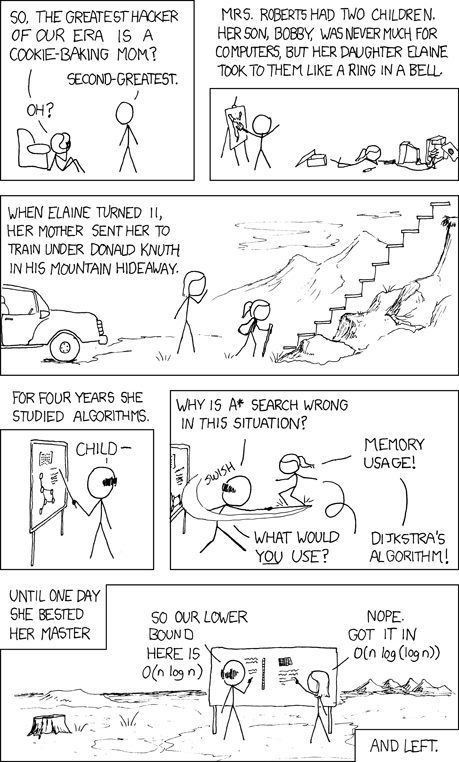
\includegraphics[keepaspectratio,width=0.8\textwidth]{elements/images/1337_part_2.png}\\
  \textline[t]{\tiny{\textit{s.\pageref{13371} $\leftarrow$ föreg.}}}{\tiny{BY-NC 2.5 xkcd.com}}{\tiny{\textit{forts. $\rightarrow$ s.\pageref{13373}}}}\par
\end{center}\par
\vspace*{-10pt}
\vfill
\null
\chapterpageimage{Avecvisor}{Avecvisor}{elements/punsch2.jpg}
\tvisa{PUNSCHHISTORIK}
\vspace{10pt}
\setlength{\parindent}{15pt}
Punschen är en likörliknande spritdryck som beredes av arrak (eller
rom), sprit, socker och vatten samt smaksättes med bland annat cognac,
rom eller whisky och eventuellt citronsaft. Namnet Punsch (eng. punch,
ursprungligen av sanskrit panca, fem, efter de ursprungliga fem
beståndsdelarna).

Den användes i Sverige första gången sannolikt 1733 vid festligheter i
anledning av hemkomsten av ostindiefararen Friederi'cus Rew Sue'ciae,
vilkens besättning i Kina lärt känna drycken och dess beredning. Till
en början förtärdes Punschen alltid varm, färdigberedd vid bordet, men
mot mitten av 1840-talet, sedan lagring (minst 4 mån) tillkommit,
vanligen kall.

Punschens kvalitet är i främsta hand beroende av arrakens beskaffenhet
samt proportionerna mellan de olika ingredienserna. Den mest
framstående punschen innehåller dock en relativt stor mängd arrak.

Den svenska fabriksmässiga punschtillverkningen daterar sig från
1845. Intill 1800-talets ingång var användningen av Punsch å allmogens
gästabud förbjuden såsom lyx.

Vissa punschtillverkare hyrde lagringsplats för sin punschfat på
svenska örlogsfartyg för att punschen skulle får lagras till sjös, man
fick en sk ``Sjörullad'' punsch.

Det sägs att Konung Karl Gustav Folke Hubertus Bernadotte spar en
skvätt punsch då han äter ärtsoppa, för att inmundiga denna senare med
de tillhörande pannkakorna.
\setlength{\parindent}{0pt}

\newpage
\tvisa{ÄRTSOPPAN}
\vspace{10pt}
Traditionen att äta ärtor just på torsdagar har sitt ursprung i de
katolska fastereglerna. Onsdagar och fredagar skulle enligt dessa
regler vara fria från kött, därför åt man på torsdagen ett riktigt
kraftigt middagsmål.

\vspace{15pt}
\fvisa{PUNSCHVISA}{Nu med en ny och stadig krök}
{\footnotesize\textit{Melodi: Med en enkel tulipan}}\\
\\
Nu med en ny och stadig krök\\
med armen gör vi försök\\
att lyfta koppen, att lyfta koppen\\
som står och väntar.\\
\\
Håll blicken fäst vid koppens rand \\
och darra inte på hand.\\
Nu allesammans, nu allesammans\\
på munnen gläntar.\\
\\
En liten punschtår så här placerad\\
i ena handen sig bättre gör\\
än tio liter uppå Systemet\\
och inga pengar att köpa för.\\
\\
Spill inga droppar på ditt bord\\
och spill ej mer några ord.\\
Nu tar vi punschen, nu tar vi punschen\\
som står och väntar

\newpage
\visa{ÄRTOR OCH PUNSCH}
{\footnotesize\textit{Melodi: Fritiof och Carmencita}}\par
\vspace{10pt}
Ärtor och punsch,\\
en liten rätt med traditioner.\\
Den smakar bra\\
och väcker många sensationer.\\
Blekgul till färgen,\\
smaken går in i märgen,\\
med en senap som blandas\\
enligt gammal tradition.\\
Så skall den njutas\\
denna svenska folks passion\\
en torsdagskväll i varje månad.\par
\vspace{10pt}
Skål vänner, bort med all tristess.\\
Ärtor och punsch ska vi njuta utan stress.\\
Inga sura miner vill vi se i afton,\\
när doften utav ärtor och punsch\\
sprids i salongen.\\
Tänk på - Grönstedt, Cederlund och Flagg,\\
åh - vilken doft från denna arraksgula tagg.\\
Hela natten ska vi njuta\\
denna underbara brygd,\\
skål för lilla ärtan och punschen.

\newpage
\visa{VI VILL HA PUNSCH}
{\footnotesize\textit{Melodi: tema ur familjen Adams}}\par
\vspace{10pt}
Vi vill ha punsch, (knäpp, knäpp)\\
vi vill ha punsch, (knäpp, knäpp)\\
vi vill ha punsch, vi vill ha punsch,\\
vi vill ha punsch. (knäpp, knäpp)\par
\vspace{10pt}
När man vill festen liva,\\
upp är det bra att kliva,\\
omkring på bordets skiva\\
och klafsa runt i punsch.\par
\vspace{10pt}
Klafsa i punsch, (slurp, slurp)\\
klafsa i punsch, (slurp, slurp)\\
klafsa i punsch, klafsa i punsch,\\
klafsa i punsch. (slurp, slurp)

\vspace{15pt}
\visa{GOLDEN DROPS}
{\footnotesize\textit{Melodi: Tomtarnas julnatt}}\\
\\
Golden drops are nice, I have reflected,\\
have reflected.\\
But their strength is not to be neglected,\\
be neglected.\\
Both your head and heart will be affected,\\
punsch, punsch, punsch!

\newpage
\fvisa{När vinet vandrat hädan}{Punsch, punsch, punsch, punsch}
{\footnotesize\textit{Melodi: Jag gick mig ut i skogen}}\par
\vspace{10pt}
\revrpt Punsch, punsch, punsch, punsch\\
punsch, punsch alla sorters\rpt\par
\vspace{10pt}
När vinet vandrat hädan\\
och maten lagts därpå\\
och kaffet står på bordet, vad väntar vi då på?\par
\vspace{10pt}
\revrpt Jo punsch, och punsch\\
och ännu mera punsch.\rpt

\vspace{15pt}
\visa{VOMMAR, VOMMAR, VOMMAR}
{\footnotesize\textit{Melodi: Sommar, sommar, sommar}}\\
\\
Vommar, vommar, vommar,\\
fyra magar har en ko.\\
Vommar, vommar, vommar,\\
kon är lycklig, må ni tro\\
För i fyra stora magar,\\
ryms all punch man behagar.\\
Vommar, vommar, vommar,\\
men så klok är ej en ko,\\
hon vill helst ha $H_2O$.

\newpage
\visa{PUNSCHEN KOMMER (KALL)}
{\footnotesize\textit{Melodi: Vals ur Glada Änkan}}\par
\vspace{10pt}
Punschen kommer, punschen kommer\\
ljuv och sval.\\
Glasen imma, röster stimma\\
i vår sal.\\
Skål för glada minnen!\\
Skål för varje vår!\\
Inga sorger finnas mer,\\
när punch vi får.

\vspace{15pt}
\visa{PUNSCHEN KOMMER (VARM)}
{\footnotesize\textit{Melodi: Vals ur Glada Änkan}}\par
\vspace{10pt}
Punschen kommer, punschen kommer\\
god och varm.\\
Vettet svinner, droppen rinner\\
ner i tarm.\\
Skål för alla minnen\\
vi snart mer ej ha,\\
då ett par glas ljuvlig punsch\\
vi hunnit ta.

\vspace{15pt}
\visa{Guling}
\vspace{10pt}
Guling, guling, kom nu lilla fuling
PUNSCH, PUNSCH, PUNSCH!

\newpage
\fvisa{TAFFELBRYTARVISA}{Till bordets fröjder och överflöd}
{\footnotesize\textit{Melodi: Nu grönskar det}}\par
\vspace{10pt}
Till bordets fröjder och överflöd\\
vi säger till sist farväl.\\
Av inre lycka och rosig glöd\\
helt stilla fylls vår själ.\\
Så lämna vi tillfälligtvis\\
det festliga bordets rund.\\
Men samlas åter glada igen efter punschen om en stund.

\vspace{15pt}
\fvisa{PUNSCHEN DET BÄSTA ÄR}{Glasen nu fyllas}
{\footnotesize\textit{Melodi: Vårvindar friska}}\par
\vspace{10pt}
Glasen nu fyllas. Punschen bör hyllas\\
såsom den är - ett livselexir!\\
Om kraften sinar, kroppen förtvinar,\\
med detta guld så finner man liv.\\
Ja, denna dryck den är vår passion.\\
En äkta vitamininjektion.\\
Man får förmoda; bland livets goda\\
punschen det bästa är!\par
\vspace{10pt}
{\footnotesize\textit{Ur spexet Unionsupplösningen från 1988 Norrlands Nation i Uppsala}}

\newpage
\fvisa{TVEKAN INFÖR PUNSCHEN}{Jag borde nog inte dricka mer}
{\footnotesize\textit{Melodi: Rosa på bal }}\par
\vspace{10pt}
Jag borde nog inte dricka mer\\
varken öl eller vin eller brännevin.\\
En kaffetår blott, men såvitt jag ser\\
står det punsch brevi'n.\par
\vspace{10pt}
Tänk vilken underbar färg och odör \\
 - nej, det blir bara man bråkar och stör.\\
Men för att inte min kväll skall bli trist,\\
krävs både slughet och list!\par
\vspace{10pt}
Så jag tror nog att jag tar en\\
punsch, kanske två, kanske tre!\\
Sen blir det groggar i baren,\\
jag klarar säkert av det!\par
\vspace{10pt}
Trots att jag egentligen är rätt knall,\\
piggar nog punsch upp mig i alla fall.\\
Jag kvicknar till med en punsch i min bål.\\
Nu har jag bestämt mig, SKÅL!

\vspace{15pt}
\fvisa{D6 90:s PUNSCHVISA}{En liten punsch helg och vardag}
{\footnotesize\textit{Melodi: Hevenu Shalom}}\par
\vspace{10pt}
En liten punsch helg och vardag.\\
En liten punsch kan ej skada.\\
En liten punsch som gör oss glada.\\
En liten punsch nån gång så där\\
emellanåt, SKÅL!!

\newpage
\fvisa{PUNSCH ELLER KONJAK}{Ska det inte bli nån punsch ikväll?}
{\footnotesize\texit{Melodi: Play a Simple Melody}}\\
\\
Ska det inte bli nån punsch ikväll?\\
Jag har väntat middan lång.\\
Punschen, kom och gör mig god och snäll.\\
Punschen kommer du nån gång?\\
\\
Punsch ger själen frid, får hjärtat slå.\\
Bra för ande och för kropp.\\
Hit med Cederlunds och Grönstedts Blå\\
och låt Flaggpunsch gå i topp.\\
\\
Punsch OK, men ingenting för mig.\\
Punschen saknar all bouqet.\\
Är det det som du har tänkt att ge\\
har jag en bättre idé.\\
\\
Ge mig konjak för det gör mig säll.\\
Courvoisier eller Martell.\\
Remy Martin det kan väl gå.\\
Annars får det bli Renault.\\
\\
{\footnotesize\texit{Vers 1 och 2 sjungs av de punsch drickande, 3 och 4 av de konjaks drickande.}}

\newpage
\fvisa{SODAVATTENPUNSCH}{Punsch punsch filibom bom bom}
{\footnotesize\textit{Melodi: Ritsch, ratsch filibom...}}\par
\vspace{10pt}
Punsch punsch filibom bom bom,\\
filibom bom bom, filibom bom bom. \\
Punsch punsch filibom bom bom,\\
filibom bom bom filibom.\\
Vi har ju både Cederlunds \\
och Carlshamns flagg\\
och Grönstedts blå och lilla Caloric\\
Det blir för tunt med sodavatten, sodavatten\\
sodavatten, blir för tunt med sodavatten\\
Ge oss mera punsch

\vspace{15pt}
\fvisa{Onomatopoetisk punsch}{Dricka på Backafall, dricker två bröder}
{\footnotesize\textit{Melodi: Flicka från Backafall}}\par
\vspace{10pt}
Dricka på Backafall, dricker två bröder.\\
Falcon gör burkar som dom fyller i.\\
Skattefritt brännvin från kusten i söder,\\
whiskey å cognac å gin, eau-de-vie.\\
Snaps kan va’ kryddad av tusende salvor\\
men jag ger bort dem varendaste en,\\
mot att få dricka av punschfirmors halvor\\
så alkoholen tar plats i var ven.\par
\vspace{10pt}
{\footnotesize\textit{Vinnande punschvisa, Karnevalen 1986}}

\newpage
\fvisa{BAILEYSVISAN}{Jag vill ej ha punsch till gasque}
{\footnotesize\texit{Melodi: Flickan i Havanna}}\\
\\
Jag vill ej ha punsch till gasque,\\
den är gul och smakar blask,\\
hellre något med choklad,\\
så kan jag bli glad.\\
\\
När jag dricker på kalas,\\
vill jag ej ha lowballglas,\\
whiskey luktar bara rök,\\
smakar gammalt ök.\\
\\
Konjak anses vara fin,\\
men är bara gammalt vin,\\
hellre då en mjölkprodukt,\\
med dess fräscha lunkt.\\
\\
Baileys är en gudadryck,\\
sjunger vi med eftertryck,\\
mjölkchoklad med sprit är bäst,\\
avrunda vår fest.

\newpage
\fvisa{LILLA PUNSCHVISAN}{Det var en gång jag tänkte att punschen övergiva}
{\footnotesize\textit{Melodi: Te deum Laudamus}}\par
\vspace{10pt}
Det var en gång jag tänkte att punschen övergiva,\\
men det får inte ske, så länge jag får leva.\\
Och när jag en gång dör, så står det på min grav:\par
\vspace{10pt}
``Här vilar en som svenska punschen älskat har''\\
Jag gillar, jag gillar punschen.\\
Jag gillar den som punschen skapat har.\\
Jag gillar, jag gillar punschen.\\
Jag gillar punschen och dess far.\par
\vspace{10pt}
{\footnotesize\textit{Ur Skogshögskolans sångbok, 1906}}

\vspace{15pt}
\visa{När kaffet är serverat}
{\footnotesize\textit{Melodi: Mössens julafton}}\par
\vspace{10pt}
När kaffet är serverat och maten tagit slut\\
och alla dom som blivit alltför fulla kastats ut.\\
då vill vi ha ett nytt glas med något gult och kallt,\\
som höjer och förbättrar vår promillehalt:\par
\vspace{10pt}
Arrak, etanol och sackaros,\\
med salt och vatten blir den bästa blandning som kan fås.\\
Söt och smetig, rent utav viskös.\\
En sexton, sjutton glas så blir man medvetslös!
\par
\vspace{10pt}
{\footnotesize\textit{Sångarstriden 1987}}

\newpage
\fvisa{PUMPA PUNSCH}{Det bryggdes en dryck uti Norden}
{\footnotesize\textit{Melodi: Albertina}}\par
\vspace{10pt}
Det bryggdes en dryck uti Norden\\
Svenska punschen så är den dryckens namn\\
BRYGGA PUNSCH!\\
Ner i vatten socker röres\\
arrak, brännvin sen tillföres\\
Svenska punschen så är den dryckens namn\\
BRYGGA PUNSCH!\par
\vspace{10pt}
Och sedan så måste drycken kylas\\
till en friskhet som nordanvind vid jul\\
KYLA PUNSCH!\\
Det skall bildas iskristaller\\
innan punschen riktigt kall är\\
med en friskhet som nordanvind vid jul\\
KYLA PUNSCH!\par
\vspace{10pt}
Lyft bägaren högt för att klinga\\
Gud bevare den gula nektars kraft\\
SKÅLA PUNSCH!\\
Den gav mod åt våra fäder\\
som bröt mark och byggde städer\\
Gud bevare den gula nektars kraft\\
SKÅLA PUNSCH!\par
\vspace{10pt}
{\footnotesize\textit{Visan härstammar från Linköpingspexet ``Darwin'', 1983.}}

\newpage
\fvisa{VÄDJAN TILL PUNSCHEN}{Kom nu lilla punschen min}
{\footnotesize\textit{Melodi: Sov du lilla videung}}\\
\\
Kom nu lilla punschen min.\\
Följ nu efter supen. \\
Snart skall du åka in\\
ner igenom strupen,\\
till mitt stora magpalats,\\
där det finns så mycket plats.\\
Kom nu lilla punschen.\\
Följ nu efter supen.

\vspace{15pt}
\visa{Varför är där ingen is till punschen?}
\vspace{10pt}
Varför är där ingen is till punschen?\\
Varför är där ingen is till punschen?\\
Varför är där ingen is till punschen?\\
Detta hände sig på den goda tiden,\\
den gamla goda tiden\\
då landet var en enda lycklig -\\
``Leve Kung Oscar!'' - idyll.\par
\vspace{10pt}
{\footnotesize\textit{Text \& musik: Povel Ramel\par
\vspace{10pt}
Förkortad version}}

\newpage
\visa{PUNSCHEN VI RADAT}
{\footnotesize\textit{Melodi: Hemåt det bär}}\par
\vspace{10pt}
Punschen vi radat upp på vårt bord\\
Ädlare dryck ej finns på vår jord.\\
Hur härligt härlig du står och väntar på mig\\
Oh, vad jag älskar dig.\par
\vspace{10pt}
{\textbf Oh ljuva punsch}\\
Oh ljuva punsch\\
{\textbf Uti min hand}\\
Uti min hand\\
{\textbf Nu tar du plats}\\
Nu tar du plats\\
{\textbf I magens famn}\\
I magens famn\\
{\textbf Jag drack dig upp}\\
Jag drack dig upp\\
{\textbf Och du rann ner}\\
Och du rann ner\\
Snart får du sällskap utav fler.\par
\vspace{10pt}
Punschen vi radat...\\
... Oh, vad du längtar ned.\par
\vspace{10pt}
{\footnotesize\textit{Sångarstriden 1978}}

\newpage
\fvisa{PUNSCHENS LOV}{Ja, punschen är och punschen var}
{\footnotesize\textit{Melodi: Rövarnas visan}}\par
\vspace{10pt}
Ja, punschen är och punschen var\\
och punschen skall förbliva.\\
En lidelse vi alla har\\
som inget kan fördriva.\\
Ja, punschen tinar opp, såväl\\
som svalkar både kropp och själ\\
Den botar begären och lindrar besvären\\
Ja, punschen den gör både gott och väl!\par
\vspace{10pt}
{\footnotesize\textit{Text: Lars-Göran\\
Från KTHs kårspex 1987, ``Sven Hedin eller en enkel tur och retur''}}

\vspace{15pt}
\fvisa{Gudars punschvisa}{Snart vi tömmer våran punch}
{\footnotesize\textit{Melodi: Sov du lilla videung}}\par
\vspace{10pt}
Snart vi tömmer våran punch\\
med en knyck på armen.\\
Punsch till frukost, punsch till lunch,\\
det är mums för tarmen!\\
Nästan hela dagarna\\
gör det gott i magarna.\\
Luta dig mot Carmen.\\
Njut i hela tarmen.

\newpage
\fvisa{FESTU:s PUNSCHVISA}{Punschen, punschen rinner nerför strupen}
{\footnotesize\textit{Melodi: Tomtarnas julnatt}}\par
\vspace{10pt}
Punschen, punschen rinner nerför strupen\\
ner för strupen.\\
Blandas, konfronteras där med supen\\
där med supen\\
Gula droppar stärker våra kroppar\\
punsch, punsch, punsch

\vspace{15pt}
\visa{HÄRLIG ÄR PUNSCHEN}
{\footnotesize\textit{Melodi: Härlig är jorden}}\par
\vspace{10pt}
Härlig är punschen,\\
härlig är dess konsistens.\\
Skönt är att taga den än en gång.\\
Genom att taga punschen av daga\\
gå vi till paradis med sång.\par
\vspace{10pt}
{\footnotesize\textit{Punschrecept\\
Ett recept för tillverkning av ca 300 liter
von Bergens Carlshamnspunsch kan ha haft följande utseende:
55 liter arrak 60\%\\
46 liter sprit 96\%\\
78 kg socker\\
157 liter vatten\\
4 liter rhenvin
kulör}}

\newpage
\fvisa{ÄNGLAPUNSCHEN}{Kalla den gudagåva eller himlanektar, vad du vill}
{\footnotesize\textit{Melodi: Änglamark}}\\
\\
Kalla den gudagåva eller himlanektar, vad du vill\\
punschen den gyllne, de gamle oss skänkte.\\
Vet att så länge som punschen nånsin funnits till\\
glädjen den höjde och sorgerna dränkte.\\
\\
Blunda och dröm om en blommande sommarnatt\\
svala bersåer där punschen står immig.\\
Eller en höstdag när Nordan har lekt tafatt\\
varm punsch som ångar och ärtsoppa simmig.\\
\\
Punschen den älskas ju av alla och en var.\\
Låt festen börja - låt punschen flöda!\\
Skål alla vänner som har nå’t i glasen kvar,\\
hedra nu minnet av gamle Kung Oscars da'r!\\
\\
Kalla den gudagåva eller himlanektar, vad du vill\\
punschen den gyllne, som får oss att drömma.\\
Fukta din strupe, låt inte flaskan stå still,\\
skåla för punschen och glasen vi tömma.

\vspace{15pt}
\fvisa{KYPAREN}{Kypar'n springer efter isen}
{\footnotesize\textit{Melodi: Räven raskar över isen}}\par
\vspace{10pt}
\revrpt Kypar'n springer efter isen.\rpt\\
\revrpt Och får han lov\rpt\\
Så tar han punschflaskan med sig.\par
\vspace{10pt}
{\footnotesize\textit{Ur sångboken från Lundakarnevalen 1990.}}

\newpage
\fvisa{BOTVISA}{Igår så drack jag punsch hela dagen}
{\footnotesize\textit{Melodi: Herrarna i hagen}}
\vspace{10pt}
Igår så drack jag punsch hela dagen\\
aj, aj, punsch hela dagen\\
ja, punsch hela dagen\par
\vspace{10pt}
Idag har jag huvudvärk och ont i magen\\
aj, aj, ont uti magen\\
ja, ont uti magen\par
\vspace{10pt}
Igår var jag glad som en kalv ut på ängen\\
aj, aj, kalv ut på ängen\\
ja, kalv ut på ängen\par
\vspace{10pt}
Idag har jag svårt att komma ur sängen\\
aj, aj, komma ur sängen\\
ja, komma ur sängen\par
\vspace{10pt}
Men nu ska jag ta mig en ny liten pärla\\
aj, aj, ny liten pärla\\
ja, ny liten pärla\par
\vspace{10pt}
Det lättar humöret, man blir fri som en ärla\\
aj, aj, fri som en ärla\\
ja, fri som en ärla

\newpage
\fvisa{DJUNGELPUNSCH}{Jag gillar alla tiders punsch}
{\footnotesize\textit{Melodi: Var nöjd med allt var livet ger.}}\\
\\
Jag gillar alla tiders punsch.\\
Punsch till frukost, punsch till lunch,\\
en punsch till förrätt, varmrätt och dessert.\\
Jag gillar punsch för vet du vad,\\
rent kaffe gör ju ingen glad.\\
Så punsch för fulla muggar vill jag ha.\\
\\
Med konjak du lockar.\\
Den bästa Renault.\\
Förlåt om jag chockar\\
och tar punsch ändå.\\
Och bjuder du på fin likör\\
får du ursäkta om det stör.\\
Jag väljer hellre Grönsteds Blå,\\
en Cederlunds eller Flaggpunsch å\\
 - kanske har du ren Platin?\\
\\
Jag gillar punsch.\\
Ger du mig punsch så är jag din.\\
För evigt din.

\vspace{15pt}
\visa{PUNSCHEN GUL}
{\footnotesize\textit{Melodi: Vem kan segla}}\\
\\
Punschen gul uppå bordet står.\\
Punschen snällt på dig vänta.\\
Om din längtan till punschen går,\\
ta den utan att flämta.

\newpage
\fvisa{LÄNGTAN TILL PUNSCHEN}{Nubben har vi tömt för länge sedan}
{\footnotesize\textit{Melodi: Längtan till landet}}\\
\\
Nubben har vi tömt för länge sedan.\\
Punschen äntligen står på tur.\\
Alla sorger har nu vikit hädan.\\
Tag en klunk och lyss till Bacchi lur.\\
Känn hur härligt allting är här i livet,\\
lundens höjder tanken närmar sig.\\
Tänk att komma bort från människolivet\\
ack, låt känslan bli evinnerlig.

\vspace{15pt}
\fvisa{SISTA PUNSCHVISAN}{När punschen småningom är slut}
{\footnotesize\textit{Melodi: Auld lange syne}}\par
\vspace{10pt}
När punschen småningom är slut\\
och vår flaska blivit tom.\\
Då vänder vi den upp och ner\\
till dess inget rinner ut.\\
\revrpt Så slickar vi så slickar vi\\
båd utanpå och i\\
och finns det ändå något kvar\\
får det va' till sämre dar.\rpt\par
\vspace{10pt}
{\footnotesize\textit{``Så slickar vi...'' kan man sjunga om och om igen tills all punsch är slut.}}

\newpage
\null
\vfill
\vspace*{-15pt}
\index{Ã1337: Part 3@1337: Part 3}
\begin{center}
  \label{13373}
  \tiny{1337: Part 3}\par
  \vspace{5pt}
  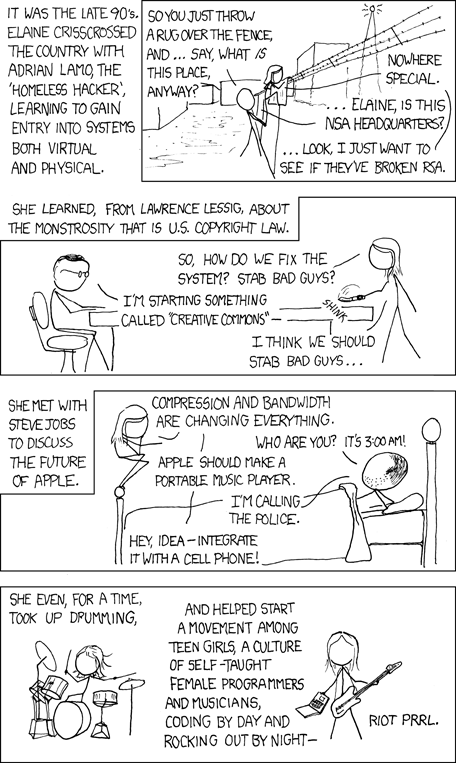
\includegraphics[keepaspectratio,width=0.8\textwidth]{elements/images/1337_part_3.png}\\
  \textline[t]{\tiny{\textit{s.\pageref{13372} $\leftarrow$ föreg.}}}{\tiny{BY-NC 2.5 xkcd.com}}{\tiny{\textit{forts. $\rightarrow$ s.\pageref{13374a}}}}\par
\end{center}\par
\vspace*{-10pt}
\vfill
\null
\chapterpageimage{Gasquevisor}{Gasquevisor}{elements/gasque.jpg}
\visa{O, GAMLA KLANG- OCH JUBELTID}
{\footnotesize\textit{Melodi: Oh alte Burschenherrlichkeit}}\par
\vspace{10pt}
O gamla klang och jubeltid\\
ditt minne skall förbliva\\
och än åt livets bistra strid,\\
ett rosigt skimmer giva.\\
Snart tystnar allt vårt yra skämt,\\
vår sång blir stum, vårt glam förstämt.\\
O, jerum, jerum, jerum.\\
O, quae mutatio rerum!\par
\vspace{10pt}
Var äro de som kunde allt,\\
blott ej sin ära svika.\\
Som voro män av äkta halt\\
och världens herrar lika?\\
De drogo bort från vin och sång\\
till vardagslivets tråk och tvång.\\
O, jerum, jerum, jerum.\\
O, quae mutatio rerum!\\
\begin{leftborder}
\begin{tabular}{l l}
  (Filosofer)  & Den ene vetenskap och vett\\		
               & in i scholares mänger,\\
  (Jurister)   & Den andre i sitt anlets svett\\
               & på paragrafer vränger,\\
  (Teologer)   & en plåstrar själen, som är skral,\\
  (Medicinare) & en lappar hop dess trasiga fodral;\\
  (Alla)       & O, jerum, jerum, jerum,\\
               & O, quae mutatio rerum!
\end{tabular}
\end{leftborder}
\newpage
Men hjärtat i en sann student,\\
kan ingen tid förfrysa.\\
Den glädjeeld, som där har tänt,\\
hans hela liv skall lysa.\\
Det gamla skalet brustit har\\
men \textit{kärnan} finnes frisk dock kvar,\\
och vad han än må mista,\\
den skall dock aldrig brista!\par
\vspace{10pt}
Så sluten, bröder, fast vår krets,\\
till glädjens värn och ära!\\
Trots allt vi tryggt och väl tillfreds,\\
vår vänskap trohet svära.\\
Lyft bägar'n högt, och klinga vän!\\
De gamla gudar leva än\\
\revrpt bland skålar och pokaler\rpt\par
\vspace{10pt}
{\footnotesize\textit{Text: August Lindh, 1925\\ Musik:
Eugen Höfling, 1825}}\par
\vspace{10pt}
{\footnotesize\textit{Vid ``kärnan' dunkas näven i bordet en
gång. Den sista versen sjungs stående samt stående på stolen, efter
sista versen sjungits sätter sig ingen åter till bords.}}

\newpage
\fvisa{VÅR UNGDOMS FAGRASTE VÅR}{Det var i vår ungdoms fagraste vår}
\vspace{10pt}
Det var i vår ungdoms fagraste vår,\\
vi drack varandra till,\\
och vi sade gutår!\\
Alla så dricka vi N.N till.\par
\vspace{10pt}
{\textbf N.N han säger inte nej därtill.}\par
\vspace{10pt}
För det var i vår ungdoms fagraste vår,\\
vi drack varandra till,\\
och vi sade gutår! 

\vspace{15pt}
\fvisa{TILL DRYCKERNAS ÄRA}{Vin är gott men öl är ljuvligt}
{\footnotesize\textit{Melodi: Här är gudagott att vara}}\par
\vspace{10pt}
Vin är gott men öl är ljuvligt\\
tänk vad snapsen värmer gott.\\
Kvällen våt och morgonen gruvlig.\\
Tänk att livet ändå är kort.\\
Punschen guldgul, konjak dito.\\
Vatten smakar inte gott.\\
Lär din läxa, drick ej lite.\\
Drick ur varje glas du fått.\par
\vspace{10pt}
{\footnotesize\textit{Text: Ove Andersson\\ Ur spexet Jämmerdal,
    1994, Norrlands Nation i Uppsala}}

\newpage
\fvisa{Mannens kläder}{Ingen har sett mannen utan kläder}
{\footnotesize\textit{Melodi: Fantomens brallor}}\par
\vspace{10pt}
Ingen har sett mannen utan kläder,\\
klädd i kostym och skor utav läder.\\
Men han blev nog frussen om sin häck,\\
om han satt på gasquen alldeles näck.\par
\vspace{10pt}
Oh, kära mannen, kliar inte sviden,\\
när du dansar på festen hela tiden.\\
Gör som damen, skaffa dig en kjol,\\
du kommer ändå alltid va' cool.\par
\vspace{10pt}
Ingen har sett honom kavla upp ärmen,\\
helsvart lekdräkt trots fukten och värmen.\\
Ibland tar han på sig ännu mer,\\
när han sig till en bal beger.\par
\vspace{10pt}
Oh, kära mannen...\par
\vspace{10pt}
{\footnotesize\textit{Text: Katarina Bergqwist}}

\newpage
\fvisa{Danse macabre}{Runt kring vår stuga smådjävlar sluga}
{\footnotesize\textit{Melodi:Vårvindar friska}}
\vspace{10pt}
Runt kring vår stuga smådjävlar sluga,\\
tassa så tyst med bockfot och svans.\\
Varulvar yla, isande kyla\\
sveper i dimma fanstygens dans.\\
Bäva, o broder, lyssna och hör\\
vrålen från gast som osalig dör.\\
Satan han skrattar, flaskan han fattar\\
super tills dagen gryr.\par
\vspace{10pt}
Gastar och spöken skymtar i kröken,\\
döingar släpar ruttnar lik.\\
Benrangel skramla, spökhänder famla,\\
kväva din strupes rosslande skrik.\\
Helvetes alla fasor släpps loss,\\
Fan rider här med hela sin tross.\\
Göm dig i stugan, du har fått flugan,\\
dille det blir din lott!

\newpage
\fvisa{INTEGRALVISAN}{En liten enkel integral}\\
{\footnotesize\textit{Melodi: Med en enkel tulipan}}\\
\\
En liten enkel integral\\
ett vektoranalystal\\
ni har besväret, ni har besväret\\
att derivera.\\
\\
Men tar man Stokes sats däruppå\\
så blir det så enkelt så\\
att integralen, att integralen\\
evaluera.\\
\\
Och rotationen, den integreras\\
sen över ytan utav en boll,\\
koordinaterna transformeras,\\
så integranden blir bara noll.\\
\\
En liten enkel integral\\
ett vektoranalystal\\
kan va så djävlig att man ej hinner\\
med något mera.

\newpage
\fvisa{KALMAREVISAN}{För uti Kalmare stad}
\vspace{10pt}
\textbf{För uti Kalmare stad}\\
ja där finns det ingen kvast\\
förrän lördagen.\\
\textbf{Hej dick}\\
Hej dack\\
\textbf{Jag slog i}\\
och vi drack\\
\textbf{Hej dickom dickom dack}\\
hej dickom dickom dack.\\
För uti Kalmare stad\\
ja där finns det ingen kvast\\
förrän lördagen.\\
\\
\revrpt \textbf{När som bonden kommer hem}\\
kommer bondekvinnan ut\rpt\\
och är stor i sin trut\\
\textbf{Hej dick...}\\
\\
\revrpt \textbf{Var är pengarna du fått?}\\
Jo, dom har jag supit opp!\rpt\\
Uppå Kalmare slott.\\
Hej dick...\\
\\
\revrpt \textbf{Jag skall mäla dig an}\\
för vår kronbefallningsman\rpt\\
Och du skall få skam\\
\textbf{Hej dick...}
\newpage
\revrpt \textbf{Kronbefallningsmannen vår}\\
satt på krogen i går\rpt\\
Och var full som ett får.\\
\textbf{Hej dick...}\\
\\
{\footnotesize\textit{Text: G S Kallstenius}}\\
\\
(\textit{Tre små tillägg})\\
\revrpt \textbf{Va' sa' bonnen ha te' mat?}\\
Sura sillar och potat\rpt\\
det blir sillsallat.\\
\textbf{Hej dick...}\\
\\
\revrpt \textbf{Säg var är din lab-rapport}\\
Jo, den har jag supit bort!\rpt\\
För den var så kort!\\
\textbf{Hej dick...}\\
\\
\revrpt\textbf{Ordföranden vår}\\
var på 100-kör igår.\rpt\\
Dom bar ut han på bår!\\
\textbf{Hej dick...}\\
\\
{\footnotesize\textit{I Linköping är det inget ``Hej dick...''-ande på
    första versen, dock reprisande som följande verser.}}

\newpage
\visa{DET VAR LÄNGE SEN}
{\footnotesize\textit{Melodi: Det var länge sin jag plocka några blommor}}\par
\vspace{10pt}
Det var länge sen jag plocka' några blommor.\\
Det var länge sen jag tog några poäng.\\
Det var länge sen jag handla' på systemet.\\
Det var länge sen jag fick en tjej/kille i säng.\par
\vspace{10pt}
Men å andra sidan bränner jag ju hemma,\\
och klarar kärleken alldeles för mig själv.\\
Det var länge sen jag plocka' några tentor\\
men å andra sidan går de om igen.

\vspace{15pt}
\fvisa{Schottis på Valhall}{Opp och hoppa Tor}
{\footnotesize\textit{Melodi: Traditionell}}\par
\vspace{10pt}
Opp och hoppa Tor, slå på trumman, bror.\\
Det är dans uppå Valhall i natt.\\
Uti Frejas sal står vår Asabal,\par
\vspace{10pt}
Opp och hoppa, fast Odin har spatt.\\
Slå i mera mjöd. Det får bli min död.\\
Nej, se där är ju Idun, min skatt.\\
Min valkyria kom hit till min midvinterrit.\\
Opp och hoppa på Valhall i natt.\par
\vspace{10pt}
Höder han hade en hiskelig hicka.\\
Balder den bota med ingefärsdricka.\\
Vred vart väl Ving-Tor, vakna och vråla.\\
Brage bråka och Skade hon skrek:\par
\newpage
Opp och hoppa...\par
\vspace{10pt}
Heimdal i hornet blåste och brumma.\\
Loke han låg där och lekte och lulla.\\
Gudarna gorma, röto och rulla.\\
Allfader Odin kvidde och kvad:\par
\vspace{10pt}
Opp och hoppa..
\par
\vspace{10pt}
{\footnotesize\textit{Text: Ulf Peder Olrog}}

\newpage
\fvisa{Båtlåt}{Det var en båt som sa till en annan}
\vspace{10pt}
Det var en båt som sa till en annan;\\
``va du va stilig. Vi borde borda varann,\\
gjorda för varann och köla lite grann,\\
som bara båtar kan.''\\
Badda bam bam bam bam\\
Badda bam bam bam.\par
\vspace{10pt}
Andra båten sa;\\
``klart att jag vill va\\
med och kryssa.\\
Kyssa din stiliga för,\\
i en stillsam slör,\\
vi varann förför.\\
som bara båtar gör.''\\
Badda bam ...\par
\vspace{10pt}
``Och när det blir lä\\
ja, då kan vi klä av oss seglen.\\
Ligga en stund vid en boj,\\
skepp o'hoj.\\
Gnida vår fernissa lite grann och fnissa,\\
kasta (t)ankar.\\
Bli lite vågade, ha lite skoj,\\
oj, oj, oj!''\par
\newpage
``Och hur vi sedan få\\
en och kanske två egna små jollar,\\
jollrande efter på släp\\
i ett navelrep,\\
e en hemlighet,\\
som bara båtar vet.''\\
Badda bam bam bam\\
Badda bam bam bam.\par
\vspace{10pt}
``Vi kan lägga till i äktenskapets hamn,\\
vid en brygga,\\
bygga ett båthus som vi kunde ligga i,\\
och tjära ner varann'\\
som bara båtar kan.''\\
Badda bam bam bam\\
som bara båtar kan\\
badda bam dam bam bam

\vspace{15pt}
\visa{VÄLKOMMEN HIT}
{\footnotesize\textit{Melodi: Jänta å ja}}\par
\vspace{10pt}
Välkommen hit, tag er en bit\\
njut utav maten vi tagit hit.\\
Skoj ska vi ha, dansa vi ska\\
trivas så där förtroligt.\\
Humöret på alla toppen ska nå\\
skratta och sjunga det ska vi få.\\
Nöjda med festen hemåt vi gå.\\
I kväll ska vi ha det roligt.

\newpage
\visa{VI SOM ÄR NYKTRA}
{\footnotesize\textit{Melodi: Du är den ende}}\par
\vspace{10pt}
Vi som är nyktra vi har faktiskt roligt.\\
Jo visst har vi ansvar, men minst lika tjolitt-\\
anlej faderulla som ni som är fulla\\
som tror ni har kul nästan jämt.\par
\vspace{10pt}
Men tänk då efter uppå dagar efter\\
de dagar med fester, med smärtsamma rester\\
utav eran hjärna, nog tycker ni gärna:\\
``Att va' nykterist är nå't visst.''\par
\vspace{10pt}
Vi som är nyktra, vi har bara roligt.\\
Imorr'n kan vi återigen ha det tjolitt-\\
anlej faderulla, men ni som var fulla\\
aj, aj, aj, det är väl för trist.

\vspace{15pt}
\fvisa{SIFFERVISAN}{1 2 sjuttiofem 6 7}
{\footnotesize\textit{Melodi: Ritsch ratsch...}}\par
\vspace{10pt}
1 2 sjuttiofem 6 7, sjuttiofem 6 7, sjuttiofem 6 7\\
1 2 sjuttiofem 6 7, sjuttiofem 6 73\\
107 103 102\\
107 6 19 27\\
17 18 16 15\\
13 19 14 17\\
19 16 15 11\\
8 42

\newpage
\visa{DOM SOM ÄR NYKTRA}
{\footnotesize\textit{Melodi: Du är den ende}}\par
\vspace{10pt}
Dom som är nyktra har inte så roligt\\
dom har bara ansvar och inte nåt tjolit-\\
an-lej-faderulla, men vi som är fulla\\
vi har bara kul nästan jämt.\par
\vspace{10pt}
Det sägs att en männ'ska kan va' utan brännvin\\
det stämmer kan hända men se blott den min\\
som pryder en absolutist den är djävligt trist\\
därför sjunger vi så:\par
\vspace{10pt}
Dom som är...

\vspace{15pt}
\visa{Inga förbud idag}
{\footnotesize\textit{Melodi: Vi går över daggstänkta berg}}\par
\vspace{10pt}
Med alla förbud i vårt land, fallera,\\
behöver vi ta ett glas ibland, fallera,\\
trots alla ritualer\\
för att köpa de pinaler\\
som kan skänka åt tillvaron glans, fallera.\\
\\
...ju mera man förbjuder\\
desto flera grytor sjuder\\
för att skänka åt tillvaron glans, fallera.\\
\\
...Fastän vinerna är dyra\\
vill vi unna oss en yra\\
och en helkväll med sång och med dans, fallera

\newpage
\fvisa{GRÅA HÅR}{Nu har vi väntat länge nog}
\vspace{10pt}
\revrpt Nu har vi väntat länge nog, 
länge nog, länge nog\rpt
Nu börjar vi få gråa hår...\\
Nu börjar vi få ATP...\\
Nu sitter vi på gravens rand...\\
Nu börjar det att lukta lik...\\
Nu bäres liken ut på bår...\\
Nu krypa vi i kistan in...\\
Nu börjar de att skyffla jord...\\
Nu har vi blivit till skelett...\\
Nu knackar vi på himlens port...\\
Nu sitter vi hos sankte Per...\\
Nu åker vi i Himlen in...\\
Nu får vi höra harpmusik...\\
Då flyr vi ner i Helvetet...\par
\vspace{10pt}
Nu capsar vi med Satan själv, Satan själv, Satan själv.\\
Nu capsar vi med Satan själv, i Helvetet.

\newpage
\visa{En gång i min ungdom festade jag}
{\footnotesize\textit{Melodi: Smedsvisa}}\par
\vspace{10pt}
En gång i min ungdom festade jag,\\
jag klämde på bordsdamens stora behag.\\
En lusing jag fick utav hennes hand\\
ur gommen flög ut en tand.\par
\vspace{10pt}
Ni alla kan se hur illa det går,\\
ni alla kan se hur illa det går.\\
När man i sin ungdom festar en dag\\
och klämmer på damers behag.\par
\vspace{10pt}
Jag tog mig en snaps mot smärtan så svår\\
och råkade trampa på kärringens tår.\\
Hon blev väl förbannad och det sa smack\\
i pannan jag fick med en klack.\par
\vspace{10pt}
Ni kan alla ...\par
\vspace{10pt}
Den klacken for in bak pannbenet mitt\\
och uti min hjärna den härjade fritt.\\
Jag hörde att värden utbringa skål,\\
och hällde en snaps i mitt hål.
\par
\vspace{10pt}
{\footnotesize\textit{Sångarstiden 1987 av E-LTH}}

\newpage
\visa{BELLMAN VINGLAR}
{\footnotesize\textit{Melodi: Fjäriln vingad...}}
\vspace{10pt}
Bellman vinglar full på haga,\\
mot en kantsten vacklar han till.\\
Alla skrattar, skrålar glada,\\
höra honnom sjunga alla vill.\\
Minsta kräk uti sin spya,\\
nyss av fylleskrålen väckt.\\
Till en ny högaktig yra,\\
stackars djävel om han flaskan spräckt.\\
\\
Uti brännvinsflaskan röjes,\\
sångarglädje, inspiration.\\
Med en djup klunk han sig nöjes,\\
rapar högt, och sedan tar han ton.\\
I en sång så glad och nöjder,\\
under bifall från sitt gäng.\\
Han besjunger flaskans fröjder,\\
alla skrålar med i hans refräng.\\
\\
Mellan päronträd och apel,\\
flåsar fram en rödsprängd snut.\\
En ilsk och tvär konstapel,\\
ordningsmakten kräver sin tribut.\\
Med en röst så sträv och sprucken,\\
Bellman ryter med ett skall:\\
``Inte fan är jag väll drucken,\\
för en sup till skulle jag stå pall.''\\
\\
Bellman släpas upp mot söder,\\
genom trånga gränder och prång.\\
Där han återser de bröder,\\
som på T-sprit håller sig i gång.\\
När han sitter på kliniken,\\
full av kryp och feta löss.\\
Han på staten är besviken:\\
``Vem har släppt in alla dessa skära möss?''

\vspace{15pt}
\visa{Åland}
{\footnotesize\textit{Melodi: Rudolf med röda mulen}} \\
\\
Åland med horn i nacken\\
han är ej som andra han\\
Svansen den går i backen\\
mulen sitter bak och fram\\
På klövarna har han skottsår\\
som hindrar honom i hans trav\\
Han hasar fram på trälår\\
med hjälp utav en gammal stav\\
\\
När älgarna drar ut på stan\\
får Åland ej va' med.\\
Han sitter vid en gammal gran\\
och täljer på sitt knä\\
Men inte har Åland hängläpp\\
Den miste han i unga år\\
Han tar sig en redig färdknäpp\\
och ringer sedan hem till Siv.

\newpage
\fvisa{PROVRÖRSBARNET}{Sov du lilla provrörsgull}
{\footnotesize\textit{Melodi: Videvisan}}\\
\\
Sov du lilla provrörsgull.\\
Nu ska Lillan sova.\\
Far din han var en ampull.\\
Vetenskapens gåva.\\
Far han fanns på institut.\\
Ur ett kylskåp togs han ut.\\
Låg där på förvaring.\\
Sov nu lilla raring.\\
\\
Jag har sluppit bli förförd,\\
skämd och chikanerad.\\
Far din, han var stamboksförd,\\
silad och filtrerad.\\
Inga kriminella drag\\
ärvda enligt Mendels lag\\
fanns i genotypen.\\
Vyssja fenotypen.\\
\\
Lugn och lycklig är din mor.\\
Vyssja lilla vännen.\\
Konkurrensen blev för stor\\
utan hjälp av männen.\\
Utan gråt och utan skratt\\
fick jag dig min lilla skatt.\\
Jag har valt tekniken\\
framför erotiken.
\newpage
Sov mitt lilla frökenbarn,\\
skönt att ha varandra.\\
Skönt att slippa dras med karl'n\\
som så många andra.\\
Oanfrätt är min moral.\\
De som sprider lömskt förtal\\
tvangs att sträcka vapen.\\
Leve vetenskapen!\\
\\
{\footnotesize\textit{Ur revyn “Nachtspiel”, 1951}}

\vspace{15pt}
\fvisa{DEN GAMLA APPARATEN}{Där som sädesbrännvin rann igenom strupen}
{\footnotesize\textit{Melodi: När som sädesfälten...}}\\
\\
Där som sädesbrännvin rann igenom strupen\\
och en flaska dunder vänta bakom den.\\
Stod den gamla apparaten uppå spisen\\
som i forna dagar var min bästa vän.\\
Så kom länsman, tog det käraste jag ägde.\\
Tog den gamla apparaten med sig hem.\\
Så nu står alla glasen tomma uppå bordet,\\
och han bränner själv, den gamle djävulen.

\newpage
\fvisa{OFVANDAHLS}{Hundra år sen ungefär}
{\footnotesize\textit{Melodi: Ovan där...}}\par
\vspace{10pt}
Hundra år sen ungefär\\
Ofvandahls han sa så här:\\
``Skriva dikter ger mig ingen\\
peng i pung, nej blott misär.\\
Det nåt annat måste bli,\\
varför inte bageri,\\
runda bullar små mig gör till millionär.''\par
\vspace{10pt}
Ofvandahls, kaffe med avec\\
Ofvandahls, Landings stora skräck,\\
Ofvandahls Napoleon canapé\\
ger oss krafter nog att vandra vidare.\par
\vspace{10pt}
Under åren som har gått,\\
många styrketåren fått\\
och en del av dem på Ofvandahls,\\
när det känns trist och grått.\\
Efter nattens hårda slit, \\
när det ej finns mera sprit,\\
då man tar en kaffetår och lever upp.\par
\vspace{10pt}
Ofvandahls, kaffe...

\newpage
\visa{Full idag}
{\footnotesize\textit{Melodi: Oh My Darling, Clementine}}\par
\vspace{10pt}
Full idag, full i möra\\
Så ser livet ut för mig\\
Jag ska aldrig lämna flaskan \\
Jag ska aldrig gifta mig\par
\vspace{10pt}
Nej, jag ska göra som dom andra\\
gå på krogen varje kväll.\\
Jag ska göra som dom andra\\
jag ska supa mig ihjäl.\par
\vspace{10pt}
Och på min gravsten\\
Och på min gravsten\\
Ska det präntas på latin\\
Att där under vilar kroppen av ett jävla fyllesvin\par
\vspace{10pt}
Och alla maskar\\
Ja alla maskar \\
som ska krypa i min kropp\\
De ska bli så jävla fulla att de aldrig hittar opp!\par
\vspace{10pt}
Skål skål alkohol\\
sånt som inte killar tål

\newpage
\fvisa{NIKOLAJEV}{Jag heter Nikolajev}
{\footnotesize\textit{Melodi: Sovjetunionens nationalsång}}\par
\vspace{10pt}
Jag heter Nikolajev\\
och kommer från Sovjet.\\
Jag flyger runt jorden\\
i min rymdraket.\\
Och där ska jag stanna i 84 varv\\
för det har Chrustjev sagt\\
men det tycker jag är larv.\par
\vspace{10pt}
Jag längtar hem, hem till min planet.\\
Till fru och barn därhemma i Sovjet.\\
Men mest utav allt längtar jag till ett rum\\
med ett hjärta på dörren.\\
Jag längtar hem till min planet\\
till fru och barn därhemma i Sovjet\par
\vspace{10pt}
Min kapsel innehåller\\
många instrument.\\
Ja, mycket av sådant\\
som ännu ej är känt.\\
Men lika förbannat, vad du än tror:\\
Jag glömde gå på muggen\\
innan jag for.\par
\vspace{10pt}
Jag längtar hem...
\par
\vspace{10pt}
{\footnotesize\textit{Uppsala teknologernas signarturmelodi, datavetare sitter ner när den sjungs.}}

\newpage
\visa{JAG HAR ALDRIG VART PÅ SNUSEN}
{\footnotesize\textit{Melodi: O hur saligt att få vandra}}\par
\vspace{10pt}
Jag har aldrig vart på snusen,\\
aldrig rökat en cigarr, halleluja!\\
Mina dygder äro tusen,\\
inga syndiga laster jag har.\\
Jag har aldrig sett nåt naket,\\
inte ens ett litet nyfött barn!\\
Mina blickar går mot taket,\\
därmed undgår jag frestarens garn, halleluja!\par
\vspace{10pt}
Halleluja...\par
\vspace{10pt}
Bacchus spelar på gitarren,\\
satan spelar på sitt handklaver!\\
Alla djävlar dansar tango,\\
säg vad kan man väl önska sig mer?\\
Jo, att alla bäckar vore brännvin,\\
Fyrisån var full av bayerskt öl.\\
Konjak i varenda rännsten\\
och punsch i varendaste pöl, mera öl!\par
\vspace{10pt}
Mera öl...\par
\vspace{10pt}

\newpage
\visa{VI KOM' FRÅN NORRLAND}
{\footnotesize\textit{Melodi: Vi bor på landet}}\par
\vspace{10pt}
Vi kom' från Norrland. Vi käkar myggen\\
som vi fångar på kalhyggen.\\
Och vi lägg' dom uppå smörgåsen\\
som vi ät' med:\\
\hspace*{25pt} laxen,\\
\hspace*{25pt} renen,\\
\hspace*{25pt} sillen,\\
\hspace*{25pt} smöre',\\
\hspace*{25pt} nubben,\\
\hspace*{25pt} kåtan,\\
\hspace*{25pt} pölsan,\\
\hspace*{25pt} pären,\\
\hspace*{25pt} fjälle',\\
\hspace*{25pt} filen,\\
\hspace*{25pt} Åkes hammock\\
 och det gör vi varje dag.\par
\vspace{10pt}
Han hette Åke och var från Tåsjö.\\
Han had' en gris som var från Blåsjö.\\
Som han lade uppå smörgåsen\\
som han käkade med laxen...\\
...och det gör han varje dag.
\newpage
Sen har vi Herman, han kom' från Böle.\\
Han hade Norrlands minsta hemman.\\
Han gick och kratte och kärringa skratte\\
så han la'na på smörgåsen\\
och han käka'na med laxen...\\
...och det gör han varje dag.\par
\vspace{10pt}
Sen har vi Göran, han kom' från Pite'\\
Har ingen hjärna men det skit' vi i.\\
För han la den uppå smörgåsen\\
som han åt med laxen...\\
...och det gör han varje dag.\par
\vspace{10pt}
Vi kom från Norrland. Ssss!\\
Vi käkar myggen Ssss!\\
som vi fångar på kalhyggen. Ssss!\\
Och vi lägg' dom Ssss!\\
uppå smörgåsen Ssss!\\
som vi ät' med laxen...\\
...och det gör vi varje daaag!

\vfill
\index{ÃParanthesis@\uppercase{Paranthesis}}
\begin{center}
  \tiny{Paranthesis}\par
  \vspace{5pt}
  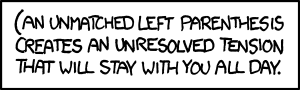
\includegraphics[keepaspectratio,width=0.6\textwidth]{elements/images/paranthesis.png}\par
  \vspace{5pt}
  \tiny{BY-NC 2.5 xkcd.com}
\end{center}
\par
\vfill
\newpage
\fvisa{Smedsvisa}{En gång i min ungdom älskade jag}
\vspace{10pt}
En gång i min ungdom älskade jag\\
en flicka med rena och sköna behag.\\
Hon lovfte mig tro, i lust och i nöd\\
allt in till sin blekaste död.\\
Hej hopp faderi faderalladerej\\
Hej hopp faderi faderalladerej\\
Hon lovfte mig tro, i lust och i nöd\\
allt in i sin blekaste död.\\
\\
Hon var som en lilja vit uti hyn\\
den vackraste kvinna man skådat i byn,\\
ett smittande skratt, en lustiger sång\\
vi älskade sommaren lång.\\
Hej hopp faderi faderalladerej\\
Hej hopp faderi faderalladerej\\
ett smittande skratt, en lustiger sång\\
vi älskade sommaren lång\\
\\
Men kärleken vissna', kärleken dog\\
vid Mikaels mässa den flickan fått nog.\\
Hon fann sig en riker och högfärdig man\\
sa ``Tack och adjö'' och försvann.\\
Hej hopp faderi faderalladerej\\
Hej hopp faderi faderalladerej\\
Hon fann sig en riker högfärdig man\\
sa ``Tack och adjö'' och försvann.\\
\\
Nu står jag vid städet sliten och grå\\
och hammaren bultar och hjärtat likså.\\
Den flickan hon kommer aldrig igen,\\
hon är hos sin nyfunne vän.\\
Hej hopp faderi faderalladerej\\
Hej hopp faderi faderalladerej\\
Den flickan hon kommer aldrig igen\\
men sången den trallar jag än.\\
Tra raj . . .
\vspace{15pt}
\fvisa{Smedsvisa den korta}{En gång i min ungdom älskade jag}
\vspace{10pt}
En gång i min ungdom älskade jag\\
sa ``Tack och adjö'' och försvann.

\vspace{15pt}
\visa{Min gode vän Joel}
{\footnotesize\textit{Melodi: Trampa på gasen}}\par
\vspace{10pt}
Min gode vän Joel,\\
han är en god kamrat,\\
han har äpplen fram\\
och en kulvert bak.\\
\\
Min gode vän Joel,\\
han ser rätt lustig ut.\\
Man kan kalla honom Knut,\\
om man vill och det vill man!
\par
\vspace{10pt}
{\footnotesize\textit{Text: Nils Dahlgren}}
\newpage
\visa{Jag ska festa}
{\footnotesize\textit{Melodi: Bamse}}\par
\vspace{10pt}
Jag skall festa, ta det lugnt med spriten.\\
Ha det roligt utan att va' full.\\
Inte krypa runt med festeliten.\\
Ta det sansat för min egen skull\\
\\
Först en öl i torra strupen,\\
efter det så kommer supen,\\
i med vinet, ner med punschen,\\
sist en groggbuffé.\\
\\
Jag är skitfull däckar först av alla,\\
missar festen, men vad gör väl det.\\
Blandar hejdlöst öl och gammalk filmjölk\\
Kastar upp på bordsdamen breve'\\
\\
Först en öl...\\
\\
Spyan rinner ner för ylleslipsen.\\
Raviolin torkar i mitt hår.\\
Vem har lagt mig under matsalsbordet?\\
Vems är gaffeln i mitt högra lår?

\newpage
\fvisa{Tacksamma visan}{Skål för den som lyssnar fast du inte pratar rent}
{\footnotesize\textit{Melodi: Halta Lottas krog}}\par
\vspace{10pt}
Skål för den som lyssnar fast du inte pratar rent\\
Skål för den som stöttar när det blivit väldigt sent\\
Skål för den som gör att det blir mera kvar till oss\\
och då menar jag förstås…\par
\vspace{10pt}
Skål för alla nykterister\\
som överser med våra brister\\
särskilt dom som är bilister\\
och kör oss hem igen\\
i gryningen
\par
\vspace{10pt}
{\footnotesize\textit{Text: Lena Olsson}}

\vspace{15pt}
\visa{Vi som oss för att glupa satt}
{\footnotesize\textit{Melodi: Vi går över daggstänkta berg}}\par
\vspace{10pt}
Vi som oss för att glupa satt, supa glatt,\\
ity den som försmå sin första tår, törsta får.\\
Av längtan att tryckas,\\
av trängtan att lyckas,\\
vi nu med bravur häller ur, eller hur?\par
\vspace{10pt}
Vi ge titt och tätt strupen sitt, supen stritt\\
skall forsa och snart får tarmen vår, varm en tår.\\
Er öven i seder\\
och söven ned Eder.\\
På denna protestbullerfest, full är bäst.

\newpage
\fvisa{SPRITROMANTIK}{Låt oss alla öppna gapet}
{\footnotesize\textit{Melodi: Mössens visa (Askungen)}}\par
\vspace{10pt}
Låt oss alla öppna gapet\\
och ge hän åt dryckenskapet.\\
För nu ska hela laget\\
va med på fylleslaget.\\
Om grannen din kollapsar\\
se till att sno \it{hans} snapsar.\\
För om du än kan stå upp\\
är det bara till att slå upp,\\
bara ställ de rosa djuren i tamburen.\\
\\
En sup ger tanken vingar,\\
skönt klingar helan går.\\
På detta vis betvingar\\
vår ångest som nyss var så svår.\\
Som sten ger på vattnet ringar\\
sprids glädjen kring, för det är visst:\\
Att supa solitä-ärt, är inte någe vä-ärt,\\
då är man ju blott en alkoholist!\\
\par
\vspace{10pt}
{\footnotesize\textit{Text: Algot Ritmer}}

\newpage
\fvisa{VIKINGEN}{En viking älskar livets vann}
{\footnotesize\textit{Melodi: When Johnny comes marching home}}\par
\vspace{10pt}
En viking älskar livets vann\\
Hurra, hurra!\\
Den hastigt i mitt svalg försvann\\
Hurra, hurra!\\
Till kalv, till oxe, till fisk, till fläsk,\\
när kärringar bara dricker läsk.\\
Ja, då vill alla vikingar ha en bäsk.\par
\vspace{10pt}
När bäsken småningom är slut\\
Tragik, tragik\\
Då bäres varje viking ut\\
som lik, sig lik\\
Och sen, om vi vaknar, vi sjunger en bit,\\
sen korkar vi upp Skånes Aquavit\\
Skål för alla vikingar som kom hit!\par
\vspace{10pt}
{\footnotesize\textit{Sångarstriden 1981 av E-LTH}}\par
\vspace{10pt}
Och datavetaren minsann,\\
vill också ha\\
en bäsk till maten då och då\\
det sitter bra\\
När datavetarens väg är klar\\
han lämnat inte en droppe har\\
skål för alla vikingar som finns kvar\par
\vspace{10pt}
{\footnotesize\textit{Text: Carl Leonardsson, Anders Steinrud, Niclas Stensbäck, Samuel Strand}}

\newpage
\visa{WE ARE SAILING}
%% {\footnotesize\textit{Melodi: Sailing}}\\
%% \\
\vspace{10pt}
We are sailing, we are sailing,\\
through the water, across the sea.\\
We are sailing, lugna waters,\\
to be ute, to be free.
\vspace{12pt}\\
\begin{tabular}{@{}m{0.1\textwidth}p{0.9\textwidth}@{}}
  \scalebox{3}{\Male} & \specialcell{I am länsing, I am glänsing,\\
    forsing framåt, mera vind!\\
    Elva meter, fulla segel,\\
    that's my life, my dear wife.}
\end{tabular}
\vspace{10pt}\\
\begin{tabular}{@{}m{0.1\textwidth}p{0.9\textwidth}@{}}
  \scalebox{3}{\Female} & \specialcell{I am freezing, it is gunging,\\
    båten laying, oh my God!\\
    Children crying, starta motor!\\
    Oh, where are we? I'll go home.}
\end{tabular}
\vspace{10pt}\\
\begin{tabular}{@{}m{0.1\textwidth}p{0.9\textwidth}@{}}
  \scalebox{3}{\Male} & \specialcell{Can't you hear me, can't you hear me?\\
    Tyst du stör mig, I am busy.\\
    I'm kappsegling, med en maxi,\\
    to be winner, or to die.}
\end{tabular}
\vspace{10pt}\\
\begin{tabular}{@{}m{0.1\textwidth}p{0.9\textwidth}@{}}
  \scalebox{3}{\Female} & \specialcell{Can't you hear me, can't you hear me?\\
    Reva segel, sun is down.\\
    Går på grundet, båt is läcking.\\
    Jag tar bussen in to town.}
\end{tabular}
\vspace{7pt}\\
We are sailing, we are sailing,\\
home again, across the sea.\\
We are flying, forever trying,\\
to be happy, to be free.

\newpage
\fvisa{MÄRTA}{Det var en flicka, hon var en snärta}
{\footnotesize\textit{Melodi: I Apladalen i Värnamo}}\par
\vspace{10pt}
Det var en flicka, hon var en snärta\\
hon bar det klingande namnet Märta.\\
Vi bruka' träffas så där ibland,\\
tills helt mitt hjärta hon satt i brand.\\
\\
En dag sa' Märta: "Ska vi spatsera\\
omkring i parken och resonera.\\
Vi kan gå runt ner på stan en stund,\\
sen får du följa mig på mitt rum."\\
\\
På ett bananskal, som låg på vägen,\\
där halka Märta, jag blev förlägen,\\
ty kan ni tänka vad jag fick se?\\
Min Märta hade ett ben av trä.\\
\\
Hom var en flicka av rätta sorten,\\
det fick jag se när vi kom till porten.\\
Hon hala klänningen upp en flik,\\
där hängde portnyckeln på en spik.\\
\\
Och när som Märta hon hade somnat,\\
och hennes träben det hade domnat,\\
jag rista' namnet i benets bark,\\
allt medan Märta i sängen snark.\\
\\
En tös med träben ska ni förvisa,\\
det har ni lärt er av denna visa.\\
Jag plocka stickor i fjorton dar,\\
och har väl alltjämt ett flertal kvar.

\vspace*{-10pt}
\newpage
\visa{Hästens rumpa}
{\footnotesize\textit{Melodi: Vintern rasat ut}}\par
\vspace{10pt}
Hästens rumpa skjuter stora bomber\\
byxor har den inte några alls.\\
När jag skyfflat skit i hekatomber\\
känner jag mig torr uti min hals.\\
Häller upp en liten jävel i glaset,\\
just som jag ska till att dricka den\\
tänker jag på jättedjuret med aset.\\
Dricker tills jag glömmer honom sen.

\vspace{15pt}
\fvisa{Flottarkärlek}{Jag var ung en gång för länge sen}
\vspace{10pt}
Jag var ung en gång för länge sen,\\
en flottare med färg.\\
Alla jäntor var som vax uti min famn.\\
I alla tork, i alla byar hade jag en liten vän\\
ifrån Norderås till skiljet ner vid Berg.\\
Haderian hadera, haderian hadera,\\
ifrån Norderås till skiljet ner vid Berg.\par
\vspace{10pt}
Jag har spelat på mitt handklaver\\
för flottare vid ån,\\
jag har spelat för små kullorna på Näs.\\
Jag har dansat över forsarna\\
med älvor och med rån,\\
medan dagen gått till ro på ängens gräs.\\
Haderian hadera, haderian hadera,\\
medan dagen gått till ro på ängens gräs.\par
\newpage
Jag har spelat sommarnätterna\\
till dans vid Rimo bro.\\
Jag har dansat med den vackra Maj i Nås.\\
Jag har svurit blonda Anna\\
evig kärlek, evig tro,\\
medan lägerelden falnat invid Ås.\\
Haderian hadera, haderian hadera,\\
medan lägerelden falnat invid Ås.\par
\vspace{10pt}
Jag ska spela på mitt bälgaspel\\
så länge jag finns till\\
i min koja invid Rekaforsens fall.\\
Jag ska drömma, jag ska älska,\\
jag ska sjunga om jag vill,\\
medan månen över moarna går vall.\\
Haderian hadera, haderian hadera,\\
medan månen över moarna går vall.

\vspace{15pt}
\visa{O HEMSKA LAB}
{\footnotesize\textit{Melodi: Julsång}}\par
\vspace{10pt}
O hemska lab, o grymma kval imorgon,\\
Här sitter jag och förstår ingenting.\\
Hela mitt inre fylls utav ett motstånd\\
Emot eländig elektrisk mätteknik.\\
Jag skulle nog behöva litet ledning,\\
Här räcker inte min kapacitans.\\
Kondensatorer och felvända dioder,\\
O hemska lab, nu vill jag koppla af.\\
O hemska lab, ty detta blir min graf!

\newpage
\fvisa{HÄRJAREVISAN}{Liksom våra fäder, vikingarna i Norden}
{\footnotesize\textit{Melodi: Gärdebylåten}}\par
\vspace{10pt}
Liksom våra fäder, vikingarna i Norden.\\
Drar vi riket runt och super oss under borden.\\
Brännvinet har blitt ett elixir,\\
för kropp såväl som själ.\\
Känner du dig liten och ynklig på jorden,\\
växer du med supen och blir stor ut i orden.\\
Slå dig för ditt håriga bröst och bli \\
en man från hår till häl.\par
\vspace{10pt}
Ja, nu skall vi ut och härja,\\
supa och slåss och svärja,\\
bränna röda stugor, slå små barn och säga fula ord.\\
Med blod skall vi stäppen färga.\\
Nu äntligen lär ja'\\
kunna dra någon riktig nytta\\
av min Hermodskurs i mord.\par
\vspace{10pt}
Hurra, nu ska man äntligen få röra benen,\\
hela stammen jublar och det spritter i grenen.\\
Tänk att än en gång få spränga fram\\
på Brunte i galopp!\\
Din doft o kära Brunte är trots sin brist i hygienen,\\
för en vild mongol minst lika ljuv som syrenen.\\
Tänk att på din rygg få rida runt\\
i stan och spela topp.\par
\vspace{10pt}
Ja, nu skall vi ut och härja...\par
\vspace{10pt}
Ja, mordbränder är klämmiga ta fram fotogenen\\
och eftersläckningen tillhör just de fenomenen\\
inom brandmansyrket som jag tycker\\
det är nån nytta med.\\
Jag målar för mitt inre upp den härliga scenen;\\
Blodrött mitt i brandgult, ej ens prins Eugen en\\
lika mustig vy kan måla, \\
ens om han målade med sked.\par
\vspace{10pt}
Ja, nu skall vi ut och härja...\par
\vspace{10pt}
{\footnotesize\textit{Text: Hans Alfredsson och Levin\\
Ur Lundaspexet Djingis Kahn 1954, första versen ej ur originalet.}}\par
\vspace{10pt}
\index{DATAVETARNAS HÄRJARVISA}
Nu ska vi kompilera,\\
supa och penetrera\\
söka rekusioner ända in\\
till fixpunktssemantik.\\
Av induktion och basfall\\
blir man med lätthet asknall.\\
Hashtabeller parsas rekursivt\\
ifrån hår till häl\par
\vspace{10pt}
{\footnotesize\textit{Text: Pär Mattsson \& Magnus Ingelbo från DVL
    Uppsala.}}

\newpage
\fvisa{Drunken Sailor}{What shall we do with the drunken sailor}
\vspace{10pt}
What shall we do with the drunken sailor,\\
what shall we do with the drunken sailor,\\
what shall we do with the drunken sailor,\\
early in the morning?\\
Hoorah! And up she rises!\\
Hoorah! And up she rises!\\
Hoorah! And up she rises!\\
Early in the morning!\par
\vspace{10pt}
Put him in the longboat 'til he's sober.\par
\vspace{10pt}
Pull out the plug and wet him all over.\par
\vspace{10pt}
Put him in the bilge and let him drink it.\par
\vspace{10pt}
Put him in a leaky boat and make him bale it.\par
\vspace{10pt}
Put him in the scupper with the hosepipe on him.\par
\vspace{10pt}
Scrape the hair off his chest with a hoop-iron razor.\par
\vspace{10pt}
Keelhaul him until he's sober\par
\vspace{10pt}
Put him in a bed with the captains daughter\par
\vspace{10pt}
Tie him to the taffrail when she's yardarm under\par
\vspace{10pt}
Heave him by the leg in a runnin' bowline.\par
\vspace{10pt}
Give 'im a dose of salt and water.

\newpage
\fvisa{CRAMBAMBOLI}{När Gud, en gång, den vackra världen skapade}
\vspace{10pt}
När Gud, en gång, den vackra världen skapade\\
så fann han allting ganska gott.\\
Han tyckte dock att Adam borde\\
få något drickbart på sin lott.\\
Så satt' han pricken över i\\
och skapade crambamboli,\\
cram-bim-bam-bamboli, crambamboli!\par
\vspace{10pt}
Napoleon, han var en tapper krigare\\
som du, som jag, som mången annan.\\
Och vet du, vad om honom sades\\
var grunden till hans tapperhet?\\
Napoleon med sitt batteri\\
han drack ett glas crambamboli,\\
cram-bim-bam-bamboli, crambamboli!\par
\vspace{10pt}
Vill du som jag hos flickor göra lycka?\\
Det kan gå bra, det kan gå galet.\\
Och vet, det är ett vågat stycke\\
som tarvar ganska mycket mod.\\
Men jag vill hålla ett mot tri\\
att hjälpa skall crambamboli,\\
cram-bim-bam-bamboli, crambamboli!\par
\vspace{10pt}
Crambamboli, ja det är jordens härlighet\\
och världens salighet förvisso.\\
En härlig dryck för tjocka magar\\
och för den magre ganska gott.\\
All världens split och tyranni\\
skall vika för crambamboli,\\
cram-bim-bam-bamboli, crambamboli!

\vspace*{-10pt}
\newpage
\fvisa{RECEPTET}{19 hönor, bruna bönor}
{\footnotesize\textit{Melodi: Gubben Noak}}\par
\vspace{10pt}
19 hönor, bruna bönor\\
18 kilogram\\
17 stycken sillar ner i magen trillar\\
16 läckra, spröda, smäckra rostade små lamm\par
\vspace{10pt}
15 bullar sedan rullar ner i halsen lätt\\
14 omeletter\\
13 fläskkotletter\\
Jag bland rätter nästan sätter dem som nummer 1\par
\vspace{10pt}
12 glas dricka kan jag slicka i mig när jag vill\\
11 små potäter jag till middag äter\\
10 gäddor\\
9 skäddor\\
8 kvistar dill\par
\vspace{10pt}
7 små harar jag väl klarar, pannekakor\\
6\\
5 små gäss med krås till\\
4 torskar, sås till\\
3 fasaner\\
2 bananer och till slut\\
1 älg. HEJ!

\newpage
\fvisa{GÄLLIVAREVISAN}{Dänkte på lörda skulle fara}\\
\vspace{10pt}\\ 
Dänkte på lörda skulle fara\\
in i Gällivare på Karakkatorg.\\
Där pjuda dricka brännvinsflaskor\\
gott som sälva satan voj, voj.\\
Det var liga liven, bara slagsmål ma niven\\
åka bolisstationen, vara jävliga fasonen.\\
Ligga inne alva natten, leva limpa å vatten\\
komma ut morrokröken, säja nappast då ajöken.\\
\\
Men dängte perkele anamma\\
ganse vara samma åka Vitafors.\\
Där sänner till en gammal licka\\
som jag prukar likka förståss.\\
De prukar pli ganska sällan, fara hälsa på fjällan\\
å ganse få lite mellan, bara inte vastna fällan.\\
De är glart man riskera, ingentin reflektera\\
bara inte nå mera, då måste gå å operera.\\
\\
Men nu jak sluta erotiken\\
öppna spritfabriken, sälja akvaviten\\
å komma lansfiskalen nära,\\
fråka om jak pära spriten.\\
De vara jävliga token, pliva hånkad av snoken\\
draka satan åt skogen, åka Luleå kroken.\\
Sitta inne halva åren, pliva krå uti håren\\
se av brännvin int spåren,\\
å komma bakas först på våren.

\newpage
\visa{Vi hade inga druvor}
{\footnotesize\textit{Melodi: Vi hade inga segel}}\par
\vspace{10pt}
Vi hade inga druvor\\
vi hade ingen råg,\\
det enda som vi hade\\
var en yxa och en såg.\\
Och så en kraftig tall\\
och efter tallens fall\\
vi kramar saften ur den\\
och tar den lagom kall.

\vspace{15pt}
\visa{När jag är fuller}
{\footnotesize\textit{Melodi: Månvisa}}\par
\vspace{10pt}
När jag är fuller, då är jag glad,\\
fan vet om jag ej är vacker.\\
Då går jag runt i vår lilla stad,\\
ibland lyxhus och baracker.\\
Jag sjunger stilla en serenad,\\
det gör jag bara när jag är glad,\\
och full och vacker, och full och vacker.\\
\\
När jag är fuller då är jag stark,\\
fan vet om jag ej är modig.\\
Då kan jag slå vem som helst i mark,\\
så han blir trasig och blodig.\\
Jag välter träden uti vår park,\\
det gör jag bara när jag är stark,\\
och full och modig, och full och modig.\\
\\
När jag är fuller då är jag rik,\\
fan vet om jag ej är snille.\\
Och dör jag blir jag ett vackert lik,\\
begravd med gravöl och gille.\\
I himlen möts jag av hornmusik,\\
det gör man bara när man är rik,\\
och är ett snille, och är ett snille\\
\\
Men om jag kvicknar till ett litet slag,\\
i något enkelrum med galler.\\
Då känner jag mig så rysligt svag,\\
och avskyr bråk och kravaller.\\
Min mage krånglar och är ur lag,\\
och fan ska veta att jag idag\\
är bakom galler, är bakom galler.
\par
\vspace{10pt}
{\footnotesize\textit{Sångartäflan 1942}}

\vspace{15pt}
\fvisa{VAR INTE BLYG}{Jag har inte fått nån sup}
{\footnotesize\textit{Melodi: Sov du lilla videung}}\\
\\
Jag har inte fått nån sup,\\
därför är jag blyger.\\
Uti magens trånga djup,\\
hämningarna smyger.\\
Men om blott jag får en tår,\\
hämningen ur kroppen går,\\
rodnar inte mera,\\
väntar blott på flera.

\newpage
\fvisa{BUSSLÅT}{Det var en buss som sa till en annan}
{\footnotesize\textit{Melodi: Båtlåt}}
\vspace{10pt}
Det var en buss som sa till en annan:\\
Va' du var stilig. Din lack é alld'less för grann.\\
Vi prejas lite grann och repar ned varann.\\
Som bara bussar kan.\\
Badda bam bam bam bam\\
Badda bam bam bam\par
\vspace{10pt}
Andra bussen sa: Klart att jag vill va'\\
med och krocka. Krossa din stiliga för.\\
Vi varann förstör. Busschauffören dör.\\
Av vägen sen vi kör.\\
Badda bam bam bam bam\\
Badda bam bam bam\par
\vspace{10pt}
Sedan kan vi slå en och kanske två\\
våldsamma volter. Landa nånstans vid en bäck.\\
Rulla lite däck. Bensintanken är läck.\\
Och elden är ej släckt.\\
Badda bam bam bam bam\\
Badda bam bam bam boom!

\newpage
\fvisa{PORTOS VISA}{Jag vill börja gasqua, var fan är min flaska}
{\footnotesize\textit{Melodi: You can't get a man with a gun, ur ``Annie get your gun''}}\par
\vspace{10pt}
Jag vill börja gasqua, var fan är min flaska,\\
vem i helvete stal min butelj.\\
Skall törsten mig tvinga en TT börja svinga,\\
men för fan bara blunda och svälj.\\
Vilken smörja, får jag spörja,\\
vem för fan tror att jag är en älg?\\
Till England vi rider och sedan vad det lider\\
träffar vi välan på någon pub.\\
Och där ska vi festa, blott dricka av det bästa,\\
utav whisky och portvin, \\
jag tänker gå hårt in\\
För att pröva på rubb och stubb.\par
\vspace{10pt}
Rubb och stubb...\par
\vspace{10pt}
{\footnotesize\textit{Text: Bergssektionen KTH\\
Det sista "stubb":et sjungs ej, enligt tradition från Linköping.}}

\vspace{15pt}
\fvisa{VÅRA FYRBENTA VÄNNER}{Mänskans bästa vän har ju fyra ben}
{\footnotesize\textit{Melodi: Bä bä vita lamm}}\par
\vspace{10pt}
Mänskans bästa vän har ju fyra ben\\
Kan de va' en gris eller va' en ren?\\
Kan de va' en tax? En katt jag fått från far?\\
Nej de är groggbordet fyllt med gin och klar.

\newpage
\fvisa{VÅRSÅNG}{Glad som en viking i offerlunden}
\vspace{10pt}
Glad som en viking i offerlunden\\
Full som en pumpa på sista april\\
Punschen i magen och lever för stunden\\
Så länge som studiestödsnämnden blott vill\par
\vspace{10pt}
Ta en poäng och sen ta sig en bläcka\\
Röja och ramla på gator och torg\\
Skändligen stans innevånare väcka\\
Slumra dan efter i lärdomens borg\par
\vspace{10pt}
Se hur med fransiga frackarna på\\
gossarna små hoppa och slå\par
\vspace{10pt}
Butter och bakis mot Heimstaden hasta\\
Lever på blodpudding pilsner och pasta\\
Och höja ett glas och sen höja ett glas\\
Som ett glatt och bekymmersfritt as.

\vspace{15pt}
\visa{KÖTTET KOMMER}
{\footnotesize\textit{Melodi: Vals ur Glada Änkan}}\par
\vspace{10pt}
...Köttet kommer, köttet kommer mört och rött.\\
Gnäggar inte springer inte, det är dött.\\
Skål för alla oxar! Skåla för varje säl.\\
Skål för alla hästar som vi slått ihjäl!\\
Raj raj raj raj raj…\par
\vspace{10pt}
{\footnotesize\textit{Text: Johan Tigrelius, Erik Hedlund,\\ David Danowsky, Linus Åkesson}}

\newpage
\fvisa{NYA STUDENTSÅNGEN}{Sjung om studentens lycklige far}
{\footnotesize\textit{Melodi: Studentsången}}\par
\vspace{10pt}
Sjungom studentens lyckliga far,\\
han kunde fröjdas i ungdomens vår!\\
Vi klappar samman i unga dar,\\
lån och pukas har grånat vårt hår.\\
Alla löften är\\
glömda för länge sen.\\
Glömt är vårt besvär,\\
men hoppas gör vi än\\
vid det löpande band som fil. kand,\\
att få bidrag till omskolningskurs!\\
att få bidrag till omskolningskurs!\\
AMS!

\vspace{15pt}
\fvisa{SI}{W kg m Wb s}
{\footnotesize\textit{Melodi: Studentsången}}\par
\vspace{10pt}
W kg m Wb s\\
$\Omega$ m T A rad\\
cd Sv N s\\
$\Omega$  A m lx dB\\
$^{\circ}$C W/$m^{2}$\\
J/kg H V C\\
kg/$m^{3}$ mol\\
m/$s^{2}$\\
m/$s^{2}$\\
F!\par
\vspace{10pt}
{\footnotesize\textit{Text: Anders Skog}}

\vspace*{-10pt}
\newpage
\visa{DANSEN GÅR PÅ SVINNSTA SKÄR}
{\footnotesize\textit{Melodi: Ljuvlig är sommarnatten}}\par
\vspace{10pt}
Dansen den går uppå Svinnsta skär,\\
hör klackarna mot hällen.\\
Gossen han svänger med flickan kär\\
i stilla sommarnatt.\\
Blommorna dofta från hagen där\\
och många andra ställen,\\
och mitt i taltrastens kvällskonsert\\
hörs många muntra skratt\par
\vspace{10pt}
Ljuvlig är sommarnatten,\\
blånande vikens vatten.\\
Och mellan bergen och tallarna\\
höres musiken och trallarna.\\
Flickan har blommor i håret,\\
månen strör silver i snåren.\\
Aldrig förglömmer jag stunderna där\\
uppå Svinnsta skär.\par
\vspace{10pt}
Gossen tar flickan uti sin hand\\
och vandrar nedåt stranden,\\
lossar sin jolle och ror från land\\
bland klippor och bland skär.\\
Drömmande ser han mot vågens rand,\\
som rullar in mot sanden,\\
kysser sin flicka så ömt ibland\\
och viskar: ''Hjärtans kär''.\par
\vspace{10pt}
Ljuvlig är sommarnatten...\par
\vspace{10pt}
Solen går upp bakom Konungssund\\
och stänker guld på vågen.\\
Fåglarna kvittra i varje lund\\
sin stilla morgonbön.\\
Gäddorna slå invid skär och grund\\
så lekfulla i hågen.\\
Men sista valsen i morgonstund,\\
man hör från Svinnerön:\par
\vspace{10pt}
Ljuvlig är sommarnatten...

\vspace{15pt}
\fvisa{KANTOM STUDIOSIJ}{Kantom studiosij extrabon sjur.}\\
{\footnotesize\textit{Melodi: Studentsången}}\\
\\
Lassom galejan in spring juvenar.\\
Noch funkar kordan kum san bravur\\
Kaj futura blondina est var\\
Nolla furii in va psykosan sit\\
Esperan vmi promissan va kredit\\
Kum voj knopa bandage in plantage\\
Kvo dullkissan diploma florit\\
Kvo dullkissan diploma florit\\
HOJLA!\\
\\
{\footnotesize\textit{In transpiranto par Ludviko Hagbaldo\\ Ur
    Grönköpings veckoblad.}}

\newpage
\fvisa{EN GLAD CALYPSO OM VÅREN}{Jag dansar runt och jag sjunger strunt}
\vspace{10pt}
Jag dansar runt och jag sjunger strunt\\
och jag är visst lite i hatten.\\
Tralalliralla i månens sken\\
där jag vandrar hemåt i natten.\\
Vart gick dom andra, var blev dom av?\\
Jag är ensam här med min flaska.\\
Tralalliralla, men det är ju kul\\
att i vattenpussarna plaska.\\
\\
Tralla-lalla-lalla-lalla.\\
Lalla-lalla-la-la.\\
Tralla-lalla-lalla-lalla-la.\\
Lalla-lalla-la-la.\\
\\
Så utmed dikena plaskar jag\\
på min stolta väg ifrån festen.\\
Tralalliralla jag trillar visst,\\
men det gör detsamma föresten.\\
Jag dansar långdans med alla trän,\\
så att mossan ryker i snåren.\\
Tralalliralla med rönn och en,\\
i en glad calypso om våren.\\
\\
Tralla...
\newpage
Jag dansa' ut på ett fält förut,\\
fullt av is som låg där och blänkte.\\
Tralalliralla precis som om\\
det var frost och snö, och jag tänkte:\\
Vad tusan frosten är svår i maj.\\
Oh, det lät som glas när jag trampa.\\
Å jädrans anamma vad jag blev skraj\\
för jag runt i drivbänkar trampa.\\
\\
Tralla...\\
\\
Men tjo, vad jag är glad ändå\\
fast jag trampat uti rabatten.\\
För det är härligt när det är vår\\
och jag dansar hemåt i natten.\\
Å, titta snart är det ljusan dag\\
alla fåglar sjunga i snåren.\\
Kom med och dansa med mig ett slag\\
i en glad calypso om våren.\\
\\
Tralla...\\
\\
{\footnotesize\textit{Text och Musik: Olle Adolphson}}

\newpage
\visa{JAG VAR FULL EN GÅNG}
{\footnotesize\textit{Melodi: Flottarkärlek}}\par
\vspace{10pt}
Jag var full en gång för länge sen,\\
på knäna kröp jag hem.\par
\vspace{10pt}
Varje dike var för mig ett vilohem.\\
I varje skåp, i varje vrå\\
hade jag en liten vän,\\
ifrån renat upp till 96 procent, procent.\par
\vspace{10pt}
Jag var full...\\
Och som sällskap hade jag en elefant.\\
Elefanten spruta vatten,\\
men jag trodde det var vin,\\
sedan dess har alla kallat mig för svin, mera vin.\par
\vspace{10pt}
Jag var full...\\
Och som sällskap hade jag en elefant.\\
Elefanten spruta vatten,\\
men jag trodde det var öl,\\
sedan dess har alla kallat mig för knöl, mera öl.\par
\vspace{10pt}
Jag var full...\\
Och som sällskap hade jag en elefant.\\
Elefanten spruta vatten,\\
men jag trodde det var sprit\\
sedan dess har alla kallat mig för skit, mera sprit

\newpage
\fvisa{Satans Tårar}{Och viljen I veta}
{\footnotesize\textit{Melodi: Viljen I veta}}\par
\vspace{10pt}
Och viljen I veta och viljen I förstå\\
hur brännvinet kommigt till världen?\\
Jo, satan försökte att Herran förmå\\
att frestas och vika för flärden.\\
Men satan han fick tji,\\
och ilsken som ett bi\\
han gav sig iväg och i ilskan han grät,\\
och tårarna hanns - det var brännvin.\\
\\
Och viljen I veta och viljen I förstå\\
hur svensken får mod uti barmen?\\
Jo, far min han fattade glaset som så,\\
och sedan så höjde han armen.\\
Han bugade sig hit,\\
han bugade sig dit,\\
så gladelig, så gladelig,\\
och hällde sen supen på tarmen.

\vspace{15pt}
\visa{FULL OCH GALEN}
{\footnotesize\textit{Melodi: Kors på Idas grav}}\par
\vspace{10pt}
Full och galen med moralen minimal.\\
Supen ger signalen till vår backanal.\\
Ritualen i lokalen är att tömma sin pokal.\\
Så skandalen i finalen är total.

\newpage
\fvisa{FAKULTATIV BACCHANAL}{Studentlivet är ett förnöjeligt stånd}
{\footnotesize\textit{Melodi: Turalleri}}\par
\vspace{10pt}
Studentlivet är ett förnöjeligt stånd.\\
Turalleri, turallera!\\
När nubbarnas bricka kring bordet gjort rond.\\
Turalleri, hurra!\\
En blomma är glädjen, i kväll slår hon ut,\\
men brännvin slås i när ditt glas tagit slut.\\
Turalleri, turallera, turalleri, hurra!\par
\vspace{10pt}
(Medicin)\\
Kvacksalvare klara Din anticeptik \\
med brännvin som snart gör baciller till lik\\
Och spara på etern, ty bättre narkos\\
av nubbarnas mångfaldigheter kan fås \par
\vspace{10pt}
(Teologi)\\
Och Du Teolog kan i smyg dricka ur \\
när inte Församlingen ser, eller hur? \\
För övrigt Vår Herre ej ogärna ser\\
sin tjänare låta en sup slinka ner .\par
\vspace{10pt}
(Juridik)\\
Det finns väl ett skäl, Du Juistitias slav, \\
att namn av brännvinsadvokat man dig gav \\
Presumptio juris det är för att Du\\
ej biter den sup som dig bjudes itu \par
\vspace{10pt}
(Filosofi)\\
Ack, Du Filosof, grå är all teori \\
Ty grön är blott snapsen som nyss slagits i \\
Och världsgåtan löses blott i alkohol\\
och visdomens kärna göms i ordet skål \par
\vspace{10pt}
Medicinare, prästmän, jurist, filosof, \\
tillsammans få trängas till sist i en strof \\
Vi mötas här alla vid bägarens rund\\
att fröjdas tillsammans en glimmande stund

\vspace{15pt}
\fvisa{SYSTEMET}{Jag kan hälsa till er från systemet}
{\footnotesize\textit{Melodi: Hälsa dem därhemma}}
\vspace{10pt}
Jag kan hälsa till er från systemet.\\
De tycker kunderna är för ivriga där.
Men en skylt skall numera lösa problemet:\\
"Drick inte ur flaskorna här!"\\
Nej, halsa dem därhemma,\\
så gör far och mor.\\
Så gör faster Elin, och lille fyllebror.\\
Halsa dem i hagen,\\
i skog, vid sjö och älv.\\
Ja, halsa dem var du vill, men inte hos oss.\\
Då får du hellre bränna själv!\\
Tjenamoss!
\vspace{10pt}
{\footnotesize\textit{Text: Povel Ramel}}

\newpage
\fvisa{SPRITBOLAGET}{Till spritbolaget ränner jag}
{\footnotesize\textit{Melodi: Emil i Lönneberga}}\\
\\
Till spritbolaget ränner jag,\\
och bankar på dess port.\\
Jag vill ha nå't som bränner bra,\\
och får mig skitfull fort.\\
Expediten sade goda',\\
hur gammal kan min herre va'.\\
Har du nåt leg, ditt fula drägg,\\
kom hit igen när du har fått skägg.\\
\\
Nej, detta var ju inte bra,\\
jag skall bli full ikväll.\\
Då plötsligt en ide jag fick,\\
de har ju sprit på Shell.\\
Många flaskor stod där på ra'.\\
Så nu kan jag bli full och gla'.\\
Den röda drycken åkte ner,\\
nu kan jag inte titta mer.\\
\\
{\footnotesize\textit{Text: Göran Svensson \\ \\ Sångarstriden 1989 av
    E-LTH.}}

\newpage
\fvisa{Reccens första}{Här kommer glasen immiga}
{\footnotesize\textit{Melodi: Fritjof Anderssons paradmarch}}\par
\vspace{10pt}
Här kommer glasen immiga med fyllning upp till rand\\
Det skall bli gott, när vi har fått\\
känna den långt ner i magen.\\
Ifall vi blir dimmiga så stödjer vi varann.\\
Lova mig att, faller jag platt\\
så tag mig uti kragen.\\
Och fröjder er nu reccar uti vårat glada gäng.\\
Att ingen får gå nykter hem att sussa i sin säng.\\
Så höjen era glas och stäm nu upp uti vårt skrål:\\
Helan är här, välkänd och kär\\
vi tar den med en SKÅL!

\vspace{15pt}
\visa{TAG NU DJUPA KLUNKAR}
{\footnotesize\textit{Melodi: Lili Marlene}}\par
\vspace{10pt}
Tag nu djupa klunkar,\\
sjung och drick, var glad.\\
Innan gänget lunkar\\
på festprisseparad.\\
Vad gör väl det om våra ben\\
då vingla lätt på gatans sten.\\
När vi beger oss hem.\\
Vi undrar blott till vem.

\chapterpageimage{Bakfyllevisor}{Bakfyllevisor}{elements/bakfylla.jpg}
\fvisa{BALLADEN DAGEN EFTER}{Han vaknade så fyllsjuk i ett främmande rum}
\vspace{10pt}
Han vaknade så fyllsjuk i ett främmande rum.\\
Aldrig hade Fredrik Åkare känt sig så dum.\\
Ty i slafen strax berdvid,\\
låg en jäntunge på glid.\\
Fröken Lind den stackars flickan\\
både barnslig och stupid.\par
\vspace{10pt}
Månens sken och dragspelstoner kan lura en man.\\
För igår när han var full var Cecilia grann.\\
Men idag i solens glans\\
ser hon ut som en schimpans.\\
Och mot kudden har hon gnidit av\\
sin forna elegans.\par
\vspace{10pt}
Vår Fredrik han är gammal men tjejen är ung.\\
Han ångrar vad han gjorde och skammen känns tung.\\
Den blir inte mindre svår\\
när han straff för otukt får.\\
För Cecilia har ljugit\\
hon är bara fjorton år.\par
\vspace{10pt}
{\footnotesize\textit{Text: Bengt Sändh}}

\newpage
\fvisa{MORALVISA}{Den som dricker mer än han tål}
{\footnotesize\textit{Melodi: Vem kan segla}}\par
\vspace{10pt}
Den som dricker mer än han tål,\\
strax runt badrummet crawlar,\\
i sitt surplus av får i kål,\\
bland roll-onnar och tvålar.

\vspace{15pt}
\visa{Snapsen var klar och kall}
{\footnotesize\textit{Melodi: Sankta Lucia}}\par
\vspace{10pt}
Snapsen var klar och kall.\\
Jag drack rätt många.\\
Strax blev jag full och knall,\\
Ågren mig fånga.\\
Nu ligger jag på dass,\\
känner mig ganska kass.\\
Ja, jag är nog dagen efter,\\
ja, dagen efter.\par
\vspace{10pt}
Aldrig, nej, aldrig mer\\
rör jag ett nubbeglas.\\
Mjölk, juice och äppelmer\\
skall jag ha på kalas.\\
Men om man tänker rätt\\
går det ju över lätt.\\
Snart så tar jag en ny pärla,\\
en liten pärla.

\newpage
\fvisa{BAKFYLLOSOFEN}{Eskimåer jagar valross}
{\footnotesize\textit{Melodi: 34:an}}\par
\vspace{10pt}
Eskimåer jagar valross.\\
Alla tyskar jagar älg.\\
Pedofiler jagar småglin.\\
Vilken värld, ja skål och svälj.\par
\vspace{10pt}
Uti skogen finns det blåbär.\\
På balkongen står en stol.\\
Uti stolen sitter jag.\\
Jag har vatt bakfull sen i fjol.\par
\vspace{10pt}
Om du hör nånting som tickar,\\
kan det kanske va en bomb.\\
Om det är en väckarklocka,\\
bara vänd och somna om.\\
Om du har en liten tax\\
och så en fet gul undulat.\\
\revrpt Ja då hopar sig problemen,\\
man kan inte ge dem samma mat.\rpt\par
\vspace{10pt}
{\footnotesize\textit{Text: Johan Tigrelius, David Danowsky,\\ Jonas Hörström, Rickard Nilsson \& Annika Svensson}}

\newpage
\visa{MJÖLK}
{\footnotesize\textit{Melodi: Trink, trink, brüderlein trink}}\par
\vspace{10pt}
\revrtp Mjölk, mjölk, vi vill ha mjölk,\\
det är en underbar dryck.\\
Mjölk, mjölk, vi vill ha mjölk,\\
det är vår senaste nyck.\\
Hämta din spann och mjölka din get\\
och ge mig en klunk utav det.\\
Slut upp i kampen för helnykterhet.\\
Mjölk är det bästa vi vet!\rpt

\vspace{15pt}
\fvisa{Ode till Treo Comp}{Morgonstund med smak av döda bävrar}
{\footnotesize\textit{Melodi: Längtan till landet}}\par
\vspace{10pt}
Morgonstund med smak av döda bävrar.\\
Frukostmorgonen är över oss.\\
Hur vi stretar, hur vi alla vägrar,\\
så går solen likt förbannat opp.\\
Snart är dagen här med hemska plågor,\\
huvudvärk och ångest, elände men\\
det finns faktiskt ett glas som dig kan hjälpa\\
Treo Comp vår frälsare och vän.

\newpage
\fvisa{KOPPARSLAGAREN 1}{Små kopparslagare här bor i staden}
{\footnotesize\textit{Melodi: En sockerbagare}}\par
\vspace{10pt}
Små kopparslagare här bor i staden\\
de är ett otyg för varje glad en.\\
De plågar stora, de plågar små,\\
de plågar många - mest dan därpå.\par
\vspace{10pt}
På förmiddagen de väcker opp en\\
med dunderslag uti huvudknoppen.\\
Sin dag de börjar med friskt humör\\
och till sin verkstad de huvet gör.\par
\vspace{10pt}
Men hettan ökar inunder pannan\\
man söker släcka med vattenkannan.\\
Man dricker mjölk och tar magnecyl\\
men ändock glöder var molekyl\par
\vspace{10pt}
Dock, kopparslagare kan man nog slippa\\
om man går nykter från var hippa\\
om man förblir vad man är helt visst\\
en pigg och skötsam absolutist.\par
\vspace{10pt}
Men vi, som lärt utav livet mera,\\
vet andra medel att den parera\\
vi har en visdom - oändligt djup;\\
vi stiger opp och tar oss en sup.

\newpage
\fvisa{KOPPARSLAGAREN 2}{En kopparslagare jag har i knoppen}
{\footnotesize\textit{Melodi: En sockerbagare}}\par
\vspace{10pt}
En kopparslagare jag har i knoppen\\
jag har försökt att på den få stopp men\\
det hjäpler inte med magnecyl\\
ej heller treo eller albyl.\par
\vspace{10pt}
Och i mitt barskåp blott tomma burkar\\
det blev helt länsat i natt av skurkar\\
som lämmnat mig här i hemmet torrt\\
med värk i huvud jag vill få bort.

\vspace{15pt}
\fvisa{Da'n därpå}{Sämre och sämre da'n därpå}
{\footnotesize\textit{Melodi: Bättre och bättre dag för dag}}\par
\vspace{10pt}
Sämre och sämre da'n därpå.\\
Säg mig, vad gjorde jag igår?\\
Många namn för hur man mår se'n\\
både bilmek, betongkeps och ågren\\
Tag, en\\
akvavitamin\\
och gå på för full maskin.\\
Aj, aj, aj, aj, aj, aj, aj\\
men jag mår sämre och sämre da'n därpå!

\newpage
\fvisa{STÖRTHÄRLIGT FULL}{Nu har alla lämnat festen}
{\footnotesize\textit{Melodi: Fat Mammy Brown}}\par
\vspace{10pt}
Nu har alla lämnat festen\\
och jag sitter ensam kvar\\
bland groggar, pilsnerflaskor\\
i en sönderslagen bar.\\
Första pilsnerflaskan tog jag\\
vid min frukost klockan fem\\
och nu sitter jag och väntar\\
på att bli buren hem.\par
\vspace{10pt}
För jag är störthärligt full.\\
Jag ramlar mest omkull.\\
Jag ser skära elefanter \\
som har jättekonstig ull.\\
Ja, jag är störthärligt full\\
och ramlar mest omkull.\\
Det är präktigt, härligt;\\
supa och va' full.\par
\vspace{10pt}
Ifrån festen minns jag inget,\\
men mitt öga blev visst blått.\\
Det måste jag ha fått\\
när någon kastat en karott\\
full med vispgrädde och fimpar\\
och en okammad peruk,\\
eller också när jag stod\\
i moraklockan och var sjuk.
\newpage
För jag är...\par
\vspace{10pt}
Nästa morgon när jag vaknar\\
med en bergsborr i min kropp\\
och sandpapper på tungan.\\
Jag vill ej stiga opp.\\
Mina armar dom känns tunga\\
och min näsa den är sne'.\\
Då raglar jag till köket\\
för en återställare.\par
\vspace{10pt}
För jag är...

\vspace{15pt}
\visa{Ont i huvudet}
{\footnotesize\textit{Melodi: Ingeborg}}\par
\vspace{10pt}
Om du har ont i huvet\\
när du vaknar någon da'\\
så häll en öl i håret\\
och låt den stå och dra.\par
\vspace{10pt}
Och känns det inte bättre\\
så skyll inte på oss,\\
Att hälla öl i huvet\\
är inte smart förstås.
\par
\vspace{10pt}
{\footnotesize\textit{Lundakarnevalen 1990}}

\newpage
\fvisa{VIT VECKA}{Jag drömmer om en vit vecka}
{\footnotesize\textit{Melodi: White christmas}}\par
\vspace{10pt}
Jag drömmer om en vit vecka\\
Sju dagar utan alkohol.\\
Tänk att bara skåla\\
i juice och cola\\
och sedan minnas allt man gjort.\par
\vspace{10pt}
Jag drömmer om en vit vecka,\\
det finns en gräns för vad jag tål.\\
Jag vill inte dricka\\
mera sprit\\
så låt nästa vecka vara vit.

\vspace{15pt}
\fvisa{ANTI-SNAPSVISA}{Huvudet vi lyfter med ett stön ur vår säng}
{\footnotesize\textit{Melodi: Sjösalavals}}\par
\vspace{10pt}
Huvudet vi lyfter med ett stön ur vår säng,\\
tvättmaskin i buken, kanoner i huvudet.\\
Tungan som en plyschsoffa och yrseln i sväng,\\
i ångesten vi svettas - kom sjung din refräng:\par
\vspace{10pt}
Varför finns det aldrig nå'n nykter karneval?\\
O, låt oss somna om så vi slipper våra kval -\\
men se, så många supar vi redan kastat upp i sängen:\\
Renat och Skåne, Svart Vinbär och fager Bäsk!

\newpage
\fvisa{Vattuvisa}{När min törst blir svår så vrider jag på kran}
{\footnotesize\textit{Melodi: Kors på Idas grav}}\par
\vspace{10pt}
När min törst blir svår så vrider jag på kran,\\
och bälgar i mig H$_2$O som fan!\\
Jag får spatten\\
utav vatten\\
Jag är bliven aquaman!\\
Bort med Skåne! Ge mig Boren, Roxen, Glan.\par
\vspace{10pt}
{\footnotesize\textit{Ur sångboken från Lunda karnevalen 1994.}}

\vfill
\index{ÃThe General Problem@\uppercase{The General Problem}}
\begin{center}
  \tiny{The General Problem}\par
  \vspace{5pt}
  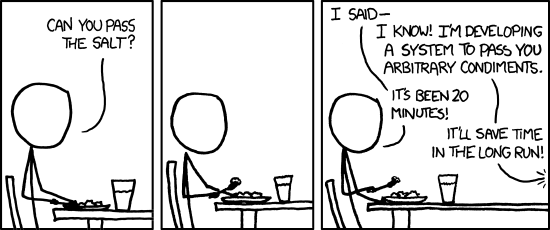
\includegraphics[keepaspectratio,width=0.9\textwidth]{elements/images/the_general_problem.png}\par
  \vspace{5pt}
  \tiny{BY-NC 2.5 xkcd.com}
\end{center}
\par
\vfill
\chapterpageimage{Säsongsvisor}{Säsongsvisor}{elements/sasong.jpg}
\fvisa{SOMMAREN �R MIN}{Och nu s� vill jag sjunga}
\vspace{10pt}
Och nu s� vill jag sjunga\\
att sommaren �r sk�n\\
och tr�den �r s� fina\\
och marken �r s� gr�n.\\
Och blommorna �r vackra\\
och h�et luktar gott\\
och solen �r s� solig\\
och vattnet �r s� v�tt.\\
Och lilla f�geln flyger\\
i boet ut och in\\
och d�rf�r vill jag sjunga\\
att sommaren �r min.\\
\\
Och jag vill ocks� sjunga\\
att fj�rilar �r bra\\
och alla s�ta myggor\\
dom vill jag ocks� ha\\
och jag �r brun om bena\\
precis som det ska va\\
och d�rf�r vill jag sjunga\\
att bruna ben �r bra.\\
Och jag har nya fr�knar\\
och prickigt sommarskin\\
och d�rf�r vill jag sjunga\\
att sommaren �r min.
\par
\vspace{10pt}
{\footnotesize\textit{Text: Astrid Lindgren\\ Musik: George Riedel}}

\newpage
\visa{DET ÄR VÅREN}
\vspace{10pt}
Det är våren, det är våren,\\
som har kommit igen\\
och med den kärleken.\\
Det är våren, ja det är våren,\\
som har kommit tillbaka igen.\\
När vi varann i portarna krama\\
och kattorna på gårdarna jama,\\
så är det våren, ja det är våren,\\
som har kommit tillbaka igen.\par
\vspace{10pt}
{\footnotesize\textit{Text: Jules Sylvain\\ Musik: Sten Hage}}

\vspace{15pt}
\fvisa{KRÄFTSNAPSEN}{Herrarna sitta, fånigt och titta}
{\footnotesize\textit{Melodi: Vårvindar friska}}\par
\vspace{10pt}
\begin{tabular}{@{}m{0.1\linewidth}p{0.8\linewidth}@{}}
  \scalebox{3}{\Female} & \specialcell{
	Herrarna sitta, fånigt och titta.\\
	Pärlorna glittra kalla som is. 
    }
\end{tabular}\par
\vspace{10pt}
\begin{tabular}{@{}m{0.1\linewidth}p{0.8\linewidth}@{}}
  \scalebox{3}{\Male} & \specialcell{
	Ja, varför dröja? Nej, låt oss höja\\
	glasen med klang på fädernas vis.\\
	Kräftpesten härjar inte i år.   
  }
\end{tabular}\par
\vspace{10pt}
Kräftfesten manar: Skål och gutår!\\
Mångubben myser, nubben den fryser.\\
Värm den i magen så att den mår.

\newpage
\fvisa{LÄNGTAN TILL LANDET}{Vintern rasat ut bland våra fjällar}
\vspace{10pt}
Vintern rasat ut bland våra fjällar\\
drivans blommor smälta ner och dö.\\
Himlen ler i vårens ljusa kvällar,\\
solen kysser liv i skog och sjö.\\
Snart är sommarn här! I purpurvågor \\
guldbelagda azurskiftande,\\
ligga ängarne i dagens lågor,\\
och i lunden dansa källorne.\\
\\
Ja, jag kommer! Hälsen glada vindar\\
ut till landet, ut till fåglarne,\\
att jag älskar dem, till björk och lindar,\\
sjö och berg, jag vill dem återse,\\
se dem än, som i min barndoms stunder,\\
följa bäckens dans till klarnad sjö,\\
trastens sång i furuskogens lunder,\\
vattenfågelns lek kring fjärd och ö.\\
\\
{\footnotesize\textit{Text: Herman Sätherberg\\ Musik: Otto Lindblad}}

\newpage
\visa{KRÄFTAN}
{\footnotesize\textit{Melodi: Räven raskar över isen}}\par
\vspace{10pt}
Kräftan lyser i karotten\\
och den största finns i botten,\\
dit ska vi ner, tills att vi ser\\
vem som till sist haver fått'en.\par
\vspace{10pt}
Uti glasen finns det vått än\\
bästa droppen finns i botten,\\
när den ska ner, ska botten upp\\
tills det går runt i kalotten.\par
\vspace{10pt}
Månen speglar sig i krusen,\\
ombesörjer gratis ljusen\\
när den går ner, då går vi opp\\
och vandrar hem lätt på snusen.

\vspace{15pt}
\fvisa{Till Kräftklon}{Med en klo som är så go}
{\footnotesize\textit{Melodi: Med en enkel tulipan}}\par
\vspace{10pt}
Med en klo som är så go\\
och en pärla jo, jo,\\
så är det bara,\\
ja det är bara att konsumera.\\
\\
Har man fått en,\\
vill man ha två,\\
och får man två är det så\\
att man vill gärna,\\
ja man vill gärna ha många flera.

\newpage
\fvisa{IDAS SOMMARVISA}{Du ska inte tro det blir sommar}
\vspace{10pt}
Du ska inte tro det blir sommar\\
ifall inte nån sätter fart\\
på sommarn och gör lite somrigt,\\
för då kommer blommorna snart.\\
Jag gör så att blommorna blommar,\\
jag gör hela kohagen grön\\
och nu så har sommaren kommit\\
för jag har just tagit bort snön.\\
\\
Jag gör mycket vatten i bäcken\\
så där så det hoppar och far.\\
Jag gör fullt med svallor som flyger\\
och myggor som svalorna tar.\\
Jag gör löven nya på träden\\
och småfågelbon här och där.\\
Jag gör himlen vacker om kvällen\\
för jag gör den alldeles skär.\\
\\
Och smultron det gör jag åt barnen,\\
för det tycker jag dom kan få,\\
och andra små roliga saker\\
som passar när barnen är små.\\
Och jag gör så roliga ställen\\
där barnen kan springa omkring,\\
då blir barnen fulla med sommar\\
och benen fulla med spring.
\par
\vspace{10pt}
{\footnotesize\textit{Text: Astrid Lindgren\\ Musik: Georg Riedel}}

\newpage
\visa{Små grodorna}
\vspace{10pt}
Små grodorna, små grodorna är lustiga att se.\\
Små grodorna, små grodorna är lustiga att se.\\
Ej öron, ej öron, ej svansar hava de.\\
Ej öron, ej öron, ej svansar hava de.\par
\vspace{10pt}
Kou ack ack ack, kou ack ack ack,\\
kou ack ack ack ack ka.\\
Kou ack ack ack, kou ack ack ack,\\
kou ack ack ack ack ka.\par
\vspace{10pt}
Små grisarna, små grisarna är lustiga att se.\\
Små grisarna, små grisarna är lustiga att se.\\
Båd svansar, båd svansar, och öron hava de.\\
Båd svansar, båd svansar, och öron hava de.\par
\vspace{10pt}
Nöff, nöff, nöff, nöff...

\vspace{15pt}
\fvisa{AVSLUTNINGSSÅNGEN}{Den studietid nu varit med tentor och projekt}\\
{\footnotesize\textit{Melodi: Den blomstertid nu kommer}}\\
\\
Den studietid nu varit med tentor och projekt\\
Det varit ganska marigt och några har den knäckt.\\
Ni andra har här samlats och nästan allt är klart.\\
Hur kan nu detta kännas om inte underbart.\\
\\
Nu kommer härlig sommar för oss som än är kvar\\
För er som nu skall knega glöm ej bort hur det var\\
med onsdagar på puben och greven som dessert\\
Ni säkert alltid ångrar att inte stanna här.

\newpage
\fvisa{Majsång}{Sköna maj}
\vspace{10pt}
Sköna maj, välkommen\\
till vår bygd igen! \\
Sköna maj, välkommen,\\
våra lekars vän!\\
Känslans gudaflamma\\
väcktes vid din ljusning;\\
jord och skyar stamma\\
kärlek och förtjusning;\\ 
sorgen flyr för våren,\\
glädje ler ur tåren,\\
morgonrodnad ur bekymrens moln.\par
\vspace{10pt}
Blomman låg förkolnad\\
under frost och snö;\\
höstens bleka vålnad,\\
gick hon nöjd att dö.\\
Vintern, härjarns like,\\ 
som föröder nejden\\
och i skövlat rike\\
tronar efter fejden,\\ 
satt med isad glaven\\
segrande på graven,\\
dyster själv och mörk och kall som den.\par
\newpage
Inga strålar sänktes\\
på vår morgon ner,\\
ingen daggtår skänktes\\
nordens afton mer,\\
tills, av svaner dragen,\\
maj med blomsterhatten\\
göt sitt guld i dagen,\\
purpurklädde natten,\\
vinterns spira bräckte\\ 
och ur lossat häkte\\
kallade den väna Flora fram.\par
\vspace{10pt}
Nu ur lundens sköte\\
och ur blommans knopp\\ 
stiga dig till möte\\
glada offer opp.\\
Blott ditt lov de susa,\\
dessa rosenhäckar,\\
till din ära brusa\\
våra silverbäckar,\\
och med tacksam tunga\\
tusen fåglar sjunga\\
liksom vi: Välkommen, sköna maj!
\par
\vspace{10pt}
{\footnotesize\textit{Text: Johan Ludvig Runeberg\\ Musik: Lars Magnus Béen}}

\newpage
\visa{VÅRVINDAR FRISKA}
\vspace{10pt}
Vårvindar friska, leka och viska,\\
lunderna kring, likt älskande par.\\
Strömmarna ila, finna ej vila,\\
förrän i havet störtvågen far.\\
Klappa mitt hjärta, klaga och hör,\\
vallhornens klang bland klipporna dör.\\
Strömkarlen spelar, sorgerna delar\\
vakan kring berg och dal.\\
\\
Hjärtat vill brista, ack, när den sista \\
gången jag hörde kärlekens röst\\
ögonens låga, avskedets plåga,\\
mun emot mun och klappande bröst.\\
Fjälldalen stod i grönskade skrud.\\
Trasten slog drill på drill för sin brud.\\
Strömkarlen spelar, sorgerna delar\\
vakan kring berg och dal
\par
\vspace{10pt}
{\footnotesize\textit{Text: Julia Nyberg\\ Folkvisa från Norrland}}

\newpage
\fvisa{VISA VID MIDSOMMARTID}{Du lindar av olvon en midsommarkrans}
\vspace{10pt}
Du lindar av olvon en midsommarkrans\\
och lägger den om ditt hår.\\
Du skrattar åt mångubbens benvita glans\\
som högt över tallen står.\\
I natt ska du dansa vid Svartrama tjärn\\
i långdans, i språngdans\\
på glödande järn.\\
I natt är du bjuden av dimman till dans\\
där Ull-Stina, Kull-Lina går.\\
\\
Nu tager du månen vid Blåbergets kam\\
att ge dig en glorias sken.\\
Och ynglet som avlas i gölarnas slam\\
blir fålar på flygande ben.\\
Nu far du till Mosslinda, Mosslunda mor,\\
där Ull-Stina, Kull-Lina, Gull-Fina bor.\\
I natt skall du somna vid Svartrama tjärn\\
där natten och mossan är len.
\par
\vspace{10pt}
{\footnotesize\textit{Text: Rune Lindström\\ Musik: Håkan Norlén}}

\newpage
\visa{SUMMARN KUMMARN}
\vspace{10pt}\\
Summarn kummar me sol,\\
kummar yvar hällmark u stain.\\
Yvar förfädars bain,\\
yvar martall yvar ain.\\
Yvar maurar u mack,\\
leiksum yvar pinnsvein u rack,\\
skeinar soli igen pa ladingen.\\
\\
Summar de jär när soli kummar yvar Austargarn\\
Summar de jär när brimsar brummar u myggar bleir me ban.\\
Summar de jär när lycku bjaudar sorgi upp till dans.\\
Visst skudd de vare trist skudd de var um summarn inte \\
fanns\\
\\
Summarn kummar...\\
\\
Vackat kan vare mosse pa en gammel sprucken stain,\\
Vackat kan var u hald si bei fast bärgningi är klain.\\
Vackat kan vare sånt som kalles fäult nån annenstans\\
Visst skudd de vare trist skudd de var um Gotland inte \\
fanns.\\
\\
Summarn kummar...\\
\\
{\footnotesize\textit{Text: Allan Nilsson\\ Musik: E Bjuresten}}

\newpage
\fvisa{Kväde till Lucian Benke}{Benke var en stalledräng}
{\footnotesize\textit{Melodi: Staffan var en stalledräng}}\par
\vspace{10pt}
Benke var en stalledräng\\
som hade liten hjärna.\\
Med sina IQ 75\\
var han ingen stjärna.\\
Handelshögen blev hans hem.\\
Han behövde aldrig mera tänka.\par
\vspace{10pt}
Vacker är han som en gud\\
och har en liten hjärna.\\
I sin konstifika skrud\\
är han ingen tärna.\\
Vår lucia då han blev.\\
Glansen från hans leende den blänka.\par
\vspace{10pt}
Med hans kropp gick upp ett ljus,\\
Benke blev en stjärna.\\
Femton kilo julesnus\\
finns det i hans hjärna.\\
Handelshögen blev hans hem.\\
Han behövde aldrig mera tänka.\par
\vspace{10pt}
Benke är en ljusets fe,\\
som har snus i hjärnan.\\
Men ingen bryr sig väl om det,\\
här uti Tavernan.\\
Handelshögen är hans hem.\\
Han behövde aldrig mera tänka.

\newpage
\visa{Kräftan är ett läckert djur}
{\footnotesize\textit{Melodi: Kovan kommer, kovan går}}\par
\vspace{10pt}
Kräftan är ett läckert djur,\\
läckert djur, läckert djur.\\
Färgen den går aldrig ur,\\
aldrig ur, aldrig ur.\\
Går den bakåt är den okokt,\\
går den framåt är det oklokt\\
att du tar en pärla till,\\
men du gör ju som du vill.\par
\vspace{10pt}
Kräftan fodrar nubbar små,\\
nubbar små, nubbar små.\\
Annars börjar den att gå,\\
den att gå, den att gå.\\
Uti magen din den kryper\\
och i tarmarna dig nyper.\\
Detta är ett ofint sätt\\
svälj nu nubben fort och lätt.

\newpage
\null
\vfill
\vspace*{-10pt}
\index{Ã1337: Part 4a@1337: Part 4a}
\begin{center}
  \label{13374a}
  \tiny{1337: Part 4a}\par
  \vspace{5pt}
  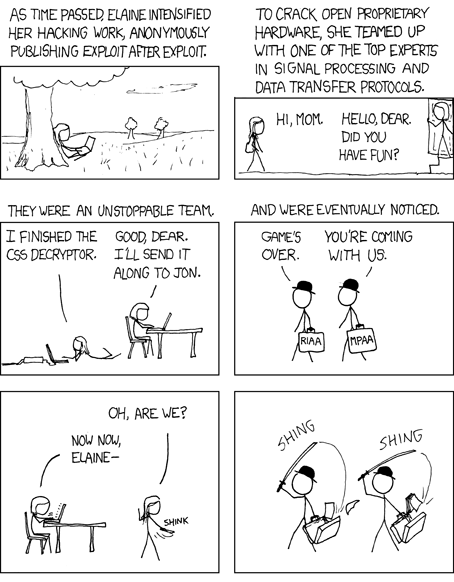
\includegraphics[keepaspectratio,width=0.8\textwidth]{elements/images/1337_part_4_1.png}\\
  \textline[t]{\tiny{\textit{s.\pageref{13373} $\leftarrow$ föreg.}}}{\tiny{BY-NC 2.5 xkcd.com}}{\tiny{\textit{forts. $\rightarrow$ s.\pageref{13374b}}}}\par
\end{center}\par
\vfill
\null
\chapterpageimage{Svenska visor}{Svenska visor}{elements/svenska.jpg}
\newpage
\tvisa{OM BELLMAN}
\vspace{10pt}
{\setstretch{0.89}\hspace{10pt} I Maria församling föddes Carl Michael
Bellman (1740-1795).  Under barndomen och ungdomens strövtåg blev Carl
Michael förtrogen med det brokiga livet på Ulla Winblads och korpral
Mollbergs söder, men hans egen barndomsmiljö var inte deras.  Bellman
gick bara en kort tid i Maria skola och undervisades sedan av
informatorer i hemmet. Familjen var inte utan lärdomstradition; Carl
Michaels farfar hade varit professor i Uppsala och hans far hade valt
ämbetsmannavägen först efter fl era utländska studieår.\par
\hspace{10pt} Att Bellman själv inte kom att leva ett vanligt borgerligt liv 
berodde på hans nöjeslystnad och ovanliga sällskapstalanger.
1760-talets Stockholm hemsöktes av en svårartad ekonomisk kris med
hastigt sjunkande penningvärde. De unga sekreterarna i ämbetsverken
roade sig på rent trots mot inf l ationen - vad tjänade det till att
spara på slantarna som för var dag blev allt mindre värda?\par
\hspace{10pt} Hemifrån hade Bellman inte heller någon hjälp att vänta. 
Familjens ekonomi undergrävdes ungefär samtidigt som sonen 1763 fl
ydde till Norge från efterhängsna fordringsägare. Från och med detta
år började hans visor spridas i huvudstaden.\par
\hspace{10pt} Snart var han åter bosatt på Söder, och i goda vänners hem 
träf f ade han stadens unga skalder som han underhöll med sin egen
märkliga talang. Och det var inte till krogar och kåkar hans talang
öppnade dörrarna, utan till grevars, riksråd och diplomaters palats -
och från och med 1772 även till kungens. 1776 fi ck han titeln
hovsekreterare och uppbar en liten ``pension'' ur kungens egen
handkassa. Samma år tillträdde han en någorlunda väl avlönad tjänst
vid Nummerlotteriet.\par}
\vspace{10pt}
{\footnotesize\textit{Ur ``Litteraturorientering för gymnasieskolan''.}}

\vspace*{-10pt}
\newpage
\visa{Bort alt hvad oro gör}
\vspace{10pt}
Bort alt hvad oro gör,\\
bort alt hvad hjertat qväljer!\\
Bäst at man väljer\\
Bland desse Bouteiller\\
Sin mag-ligueur.\\
\revrpt Granne! gör du just som jag gör,\\
Vet denna oljan ger humeur.\\
Hvad det var läckert!\\
Hvad var det? Renskt Bläckert?\\
	Oui Monseigneur.\rpt\\
\\
Bort alt hvad oro gör,\\
Alt är ju stoft och aska,\\
Lät oss bli raska,\\
Och tömma vår flaska\\
Bland Bröderna.\\
\revrpt Granne! gör du just som jag gör,\\
Vet denna oljan ger humeur.\\
Hvad det var mägtigt!\\
Hva var det? ... Jo präktigt,\\
	Mallaga - ja.\rpt

\newpage
\fvisa{Fredmans Epistel N:o 2 - Til Fader Berg, rörande Fiolen}{Nå Skruvfa Fiolen}
\\
Nå skrufva Fiolen,\\
Hej! Spelman skynda dej.\\
Kära Syster, hej!\\
Svara inte nej,\\
Svara Ja så bli Vi glada.\\
Sätt dej du på stolen,\\
Och stryk din Silfversträng;\\
Röda stråken släng,\\
Och med armen sväng;\\
Gör ej fiolen skada.\\
Du svettas, stor sak,\\
I Bränvin skall du bada;\\
Ty under detta Tak\\
Är Bacchi Lada.\\
-  -  Ganska rigtigt,\\
Ditt kall är vigtigt\\
Båd för Öra, Syn och Smak.\\
\\
Bland Nymphernas skara\\
Är du omistlig man;\\
Du båd vill och kan\\
Mer än någon ann\\
De unga hjertan binda,\\
Och kärlekens snara\\
På dina strängar står;\\
Hvarje Ton du slår,\\
Du et hjerta får,\\
At konstigt sammanlinda.\\
Just på en minut,\\
Små ögon blifva blinda,\\
Och flickorna til slut\\
De bli så trinda.\\
-  -  Hur du bullrar!\\
Men Nymphen kullrar,\\
Och du skrattar med din trut.\\
\\
Jag älskar de sköna,\\
Men Vinet ändå mer;\\
Jag på båda ser,\\
Och åt båda ler\\
Men skiljer ändå båda.\\
En Nymph i det gröna,\\
Och Vin i gröna glas:\\
Lika godt Calas,\\
Båda om mig dras.\\
Ge stråken mera kåda;\\
Confonium tag där\\
Uti min gröna Låda;\\
Och Vinet står ju här.\\
Jag är i våda.\\
-  -  Supa, dricka,\\
Och ha sin flicka,\\
Är hvad Sancte Fredman lär.

\newpage
\fvisa{Fredmans Epistel N:o 9}{Käraste bröder, systrar och vänner}
{\footnotesize\textit{Till Gumman på Thermopilum Boreale och hennes jungfrur.}}\par
\vspace{10pt}
Käraste bröder, systrar och vänner,\\
Si fader Berg han skruvar och spänner\\
Strängarna på fiolen och stråken han tar i hand.\\
Ögat är borta, näsan är kluven;\\
Si hur han står och spottar på skruven;\\
Ölkannan står på stolen;\\
Nu knäpper han litet grand;\\
- Grinar mot solen,\\
- Pinar fiolen,\\
Han sig förvillar, drillar ibland.\\
Käraste bröder, dansa på tå,\\
Handskar i hand och hattarna på.\\
Si på jungfru Lona, röda band i skona,\\
Nya strumpor himmelsblå.\par
\vspace{10pt}
Si Jergen Puckel fläktar med hatten,\\
Pipan i mun, och brännvin som vatten\\
Dricker han och gör fukter med huvud och hand och fot;\\
Guldguler rock med styva ducriner;\\
Tätt uti nacken hårpiskan hänger;\\
Ryggen i hundra bukter och kindbenen stå som klot;\\
- Gapar på noten,\\
- Skrapar med foten,\\
Pipan han stoppar, hoppar emot.\\
Käraste systrar, alltid honnett;\\
Bröderna dansa jämt menuett, hela natten fulla.\\
Rak i livet, Ulla,\\
Ge nu hand, håll takten rätt!\par
\vspace{10pt}
Si vem är det i nattrock så nätter,\\
Med gula böxor, vita stövletter,\\
Som dansar där med Lotta,\\
Den där som har röd peruk?\\
Ta mej sju tusen, se två i flocken,\\
Sydda manschetter, snören på rocken.\\
Drick, fader Berg, och spotta!\\
Tvi, svagdricka gör mig sjuk.\\
- Kruset ska rinna;\\
- Huset ska brinna,\\
Ingen ska klämta. Flämta, min buk!\\
Käraste systrar, tagen i ring,\\
Dansa och fläkta, tumla och spring!\\
Var nu blind och döver!\\
Spelman ger nu över, raglar med fiolen kring.\par
\vspace{10pt}
Hej, mina flickor lyfta på kjolen,\\
Dansa och skratta! Hör basfiolen!\\
Ge fader Berg konfonium\\
Och hoglands med gröna blan!\\
Hör, fader Berg säg du, vad hon heter,\\
Hon där vid skänken vindögd och feter!\\
Gumman på Thermopolium, hon är det, ja ta mig fan.\\
- Trumpen och blinder,\\
- Gumpen är trinder,\\
Halsfräs, min gumma! Brumma, dulcian!\\
Käraste bröder, här är behag,\\
Här är musik och flickor var dag,\\
Här är Bacchus buden, här är kärleksguden,\\
Här är allting, här är jag.\par
\vspace{10pt}
{\footnotesize\textit{Text \& Musik: Carl Michael Bellman}}

\vspace*{-10pt}
\newpage
\fvisa{Fredmans Epistel N:\lowercase{o} 81}{Märk, hur' vår skugga, märk, Movitz mon Frère}
{\footnotesize\textit{Till grälmakar Löfberg i stärbhuset vid Dantobommen, diktad vid graven.}}\par
\vspace{10pt}
Märk, hur' vår skugga, märk, Movitz mon Frère,\\
inom ett mörker sig slutar,\\
hur guld och purpur i skoveln, den där,\\
byts till grus och klutar.\\
Vinkar Charon från sin brusande älv,\\
och tre gånger sen dödgrävaren själv,\\
mer du din druva ej kryster.\\
Därföre Movitz kom hjälp mig och välv\\
gravsten över vår syster!\par
\vspace{10pt}
Ack längtansvärda och bortskymda skjul\\
under de susande grenar,\\
där tid och döden en skönhet och ful\\
till ett stoft förenar!\\
Till dig aldrig avund sökt någon stig;\\
lyckan, eljest uti flykten så vig,\\
aldrig kring grifterna ilar.\\
Ovän där väpnad, vad synes väl dig?\\
bryter fromt sina pilar.\par
\newpage
Lillklockan klämtar till storklockans dön,\\
lövad står kantorn i porten\\
och vid de skrålande gossarnas bön\\
helgar denna orten.\\
Vägen opp till templets griftprydda stad\\
trampas mellan rosors gulnade blad,\\
multnade plankor och bårar;\\
till dess den långa och svartklädda rad,\\
djupt sig buga med tårar.\par
\vspace{10pt}
Så gick till vila, från slagsmål och bal,\\
grälmakar Löfberg, din maka,\\
där, dit åt gräset långhalsig och smal\\
du än glor tilbaka.\\
Hon från Dantobommen skildes i dag,\\
och med henne alla lustiga lag.\\
vem skall nu fl askan befalla?\\
Torstig var hon och uttorstig är jag;\\
vi ä torstiga alla.\par
\vspace{10pt}
{\footnotesize\textit{Text \& Musik: Carl Michael Bellman}}

\newpage
\fvisa{Fredmans Epistel N:o 82}{Vila vid denna källa}
{\footnotesize\textit{eller Oförmodade avsked, förkunnat uid Ulla Winblads 
frukost en\\sommarmorgon i det gröna}}\par
\vspace{10pt}
Vila vid denna källa,\\ 
Vår lilla Frukost vi framställa:\\ 
Rödt Vin med Pimpinella\\ 
Och en nyss skuten Beccasin.\\ 
Klang hvad Buteljer, Ulla! \\ 
I våra Korgar öfverstfulla,\\ 
Tömda i gräset rulla,\\ 
Och känn hvad ångan dunstar fin,\\ 
Ditt middags Vin\\ 
Sku vi ur krusen hälla,\\ 
Med glättig min.\\ 
Hvila vid denna källa,\\ 
Hör våra Valdthorns klang Cousine.\\ 
Valdthornens klang Cousine.\par
\vspace{10pt}
Prägtigt på fältet pråla,\\ 
Än Hingsten med sitt Sto och Fåla,\\ 
Än Tjurn han höres vråla,\\ 
Och stundom Lammet bräka tör;\\ 
Tuppen på taket hoppar,\\ 
Och liksom Hönan vingen loppar,\\ 
Svalan sitt hufvud doppar,\\ 
Och Skatan skrattar på sin stör.\\ 
Lyft Kitteln; hör.\\ 
Lät Caffe-glöden kola,\\ 
Där nedanför.\\ 
Prägtigt på fältet pråla\\  
De ämnen som mest ögat rör.\\ 
Som mest vårt öga rör.\par
\vspace{10pt}
Himmel! hvad denna Runden,\\ 
Af friska Löfträn sammanbunden,\\ 
Vidgar en plan i Lunden,\\ 
Med strödda gångar och behag.\\ 
Ljufligt där löfven susa,\\ 
I svarta hvirflar grå och ljusa,\\ 
Träden en skugga krusa,\\ 
Inunder skyars fläkt och drag.\\ 
Tag, Ulla tag,\\ 
Vid denna måltids stunden,\\ 
Ditt glas som jag.\\ 
Himmel! hvad denna Runden,\\ 
Bepryds af blommor tusen slag!\\ 
Af blommor tusen slag.\par
\vspace{10pt}
Nymphen, se hvar hon klifver,\\ 
Och så beställsam i sin ifver,\\ 
Än Ägg och än Oliver,\\ 
Uppå en rosig tallrik bär.\\ 
Stundom en sked hon öser,\\ 
Och öfver Bunken gräddan slöser;\\ 
Floret i barmen pöser,\\ 
Då hon den Mandeltårtan skär.\\ 
En Kyckling där,\\ 
Af den hon vingen rifver,\\ 
Nyss kallnad är.\\ 
Nymphen se hvar hon klifver,\\ 
Och svettas i et kärt besvär.\\ 
Och svettas i besvär.\par
\vspace{10pt}
Blåsen J Musikanter,\\ 
Vid Eols blåst från berg och branter;\\ 
Sjungen små Kärleks-Panter,\\ 
Bland gamla Mostrars kält och gnag.\\ 
Syskon! en sup vid disken,\\ 
Och pro secundo en på Fisken;\\ 
Krögarn, den Basilisken,\\ 
Summerar Taflan full i dag.\\ 
Klang Du och Jag!\\ 
Klang Ullas amaranther,\\ 
Af alla slag!\\ 
Blåsen J Musicanter,\\ 
Och hvar och en sin kallsup tag.\\ 
Hvar en sin kallsup tag.\par
\vspace{10pt}
Ändtlig i detta gröna,\\ 
Får du mitt sista afsked röna;\\ 
Ulla! farväl min Sköna,\\ 
Vid alla Instrumenters ljud.\\ 
Fredman ser i minuten\\ 
Sig til Naturens skuld förbruten,\\ 
Clotho ren ur Surtouten,\\ 
Afklipt en knapp vid Charons bud.\\ 
Kom hjertats Gud!\\ 
At Fröjas ätt belöna\\ 
Med Bacchi skrud.\\ 
Ändtlig i detta gröna,\\ 
Stod Ulla sista gången Brud.\\ 
Den sista gången Brud.\par
\vspace{10pt}
{\footnotesize\textit{Text \& Musik: Carl Michael Bellman}}

\newpage
\fvisa{Fredmans Sång N:o 10}{Supa klockan öfver tolf}
\vspace{10pt}
Supa klockan öfver tolf,\\
Lefva bland förryckta!\\
Jorden är mitt kammargolf,\\
Solen är min lyckta!\\
Jag bryr mig om ingenting,\\
Blott at hjernen löper kring \\
	Löper kring\\
	Löper kring\\
	Löper kring\\
	Löper kring,\\
Intil dess hon domnar,\\
Och jag fattig somnar.\\
	 \\
I min Farfars gamla rock,\\
Hål uppå armbågen,\\
Står jag bland en lustig flock,\\
Super bara rågen,\\
Tar mig ur de vackra krus\\
Morgon-, middags-, afton-rus\\
	 Afton-rus\\
	 Afton-rus\\
	 Afton-rus\\
	 Afton-rus,\\
Och så blir jag röder\\
Som de ägta bröder.\\

Stode salig Far min opp,\\
Och mig hörde hicka,\\
Sade han: min gosse, topp!\\
Vi sku brorskål dricka.\\
Ja min Bror, så svarte jag:\\
Drick med mig til ljusan dag\\
	 Ljusan dag\\
	 Ljusan dag\\
	 Ljusan dag\\
	 Ljusan dag,\\
Sedan må du ila\\
Åter til din hvila.\\
\\

Blefve jag en riker man,\\
Finge mynt i pungen,\\
Skulle jag til Jul min sann,\\
Klä mig grann som Kungen,\\
Köpa mig förr'n någon tror,\\
Rock och väst och nya skor,\\
	 Nya skor\\
	 Nya skor\\
	 Nya skor\\
	 Nya skor,\\
Och så pung i håret,\\
Och så ur på låret.\\
	 \\

Men min strupe vil bli full,\\
Tål ej denna torken;\\
Guld ej annat är än mull,\\
Gubbar ta ur korken;\\
Låtom oss i ro och fred\\
Svälja sista klunken ned,\\
	Klunken ned\\
	Klunken ned\\
	Klunken ned\\
	Klunken ned,\\
Och oss sedan döda\\
I det våta röda.

\newpage
\fvisa{Fredmans Sång N:o 21}{Så lunka vi så småningom}
{\footnotesize\textit{Måltidssång}}\par
\vspace{10pt}
Så lunka vi så småningom\\
Från Bacchi buller och tumult,\\
När döden ropar, Granne kom,\\
Ditt timglas är nu fullt.\\
Du Gubbe fäll din krycka ner,\\
Och du, du Yngling, lyd min lag,\\
Den skönsta Nymph som åt dig ler\\
Inunder armen tag.\\
Tycker du at grafven är för djup,\\
Nå välan så tag dig då en sup,\\
Tag dig sen dito en, dito två, dito tre,\\
Så dör du nöjdare.\par
\vspace{10pt}
Du vid din remmare och präss,\\
Rödbrusig och med hatt på sned,\\
Snart skrider fram din likprocess\\
I några svarta led;\\
Och du som pratar där så stort,\\
Med band och stjernor på din rock,\\
Ren snickarn kistan färdig gjort,\\
Och hyflar på des lock.\\
Tycker du...\par
\newpage
Men du som med en trumpen min,\\
Bland riglar, galler, järn och lås,\\
Dig hvilar på ditt penningskrin,\\
Innom din stängda bås;\\
Och du som svartsjuk slår i kras\\
Buteljer, speglar och pocal;\\
Bjud nu god natt, drick ut dit glas,\\
Och helsa din rival;\\
Tycker du...\par
\vspace{10pt}
Och du som under titlars klang\\
Din tiggarstaf förgylt hvart år,\\
Som knappast har, med all din rang,\\
En skilling til din bår;\\
Och du som ilsken, feg och lat,\\
Fördömmer vaggan som dig hvälft,\\
Och ändå dagligt är placat\\
Til glasets sista hälft;\\
Tycker du...\par
\vspace{10pt}		  
Du som vid Martis fältbasun\\
I blodig skjorta sträckt ditt steg;\\
Och du som tumlar i paulun,\\
I Chloris armar feg;\\
Och du som med din gyldne bok\\
Vid templets genljud reser dig,\\
Som rister hufvud lärd och klok,\\
Och för mot afgrund krig;\\
Tycker du...\par
\vfill
\hfill {\footnotesize\textit{forts. $\rightarrow$}}
\newpage
Men du som med en ärlig min\\
Plär dina vänner häda jämt,\\
Och dem förtalar vid dit vin,\\
Och det liksom på skämt;\\
Och du som ej försvarar dem,\\
Fastän ur deras flaskor du,\\
Du väl kan slicka dina fem,\\
Hvad svarar du väl nu?\\
Tycker du...\par
\vspace{10pt}
Men du som til din återfärd,\\
Ifrån det du til bordet gick,\\
Ej klingat för din raska värd,\\
Fastän han ropar: Drick!\\
Drif sådan gäst från mat och vin,\\
Kör honom med sitt anhang ut,\\
Och sen med en ovänlig min,\\
Ryck remmarn ur hans trut.\\
Tycker du...\par
\vspace{10pt}				   
Säg är du nöjd? min granne säg,\\
Så prisa värden nu til slut;\\
Om vi ha en och samma väg,\\
Så följoms åt; drick ut.\\
Men först med vinet rödt och hvitt\\
För vår Värdinna bugom oss,\\
Och halkom sen i grafven fritt,\\
Vid aftonstjernans bloss.\\
Tycker du...\par
\vspace{10pt}
{\footnotesize\textit{Text \& Musik: Carl Michael Bellman}} 

\newpage
\fvisa{Fredmans Sång N:\lowercase{o} 35}{Gubben Noach, Gubben Noach}
\vspace{10pt}
\revrpt Gubben Noach, Gubben Noach\\ 
Var en hedersman,\rpt \\ 
När han gick ur arken\\ 
Plantera han på marken\\ 
Mycket vin, ja mycket vin, ja\\ 
Detta gjorde han.\par
\vspace{10pt}
\revrpt Noach rodde, Noach rodde\\ 
Ur sin gamla ark,\rpt \\ 
Köpte sig buteljer,\\ 
Sådana man sälljer,\\ 
För at dricka, för at dricka\\ 
På vår nya park.\par
\vspace{10pt}
\revrpt Han väl visste, han väl visste\\ 
At en mänska var\rpt \\ 
Torstig af naturen\\ 
Som de andra djuren,\\ 
Därför han ock, därför han ock\\ 
Vin planterat har.\par
\vspace{10pt}
\revrpt Inga skålar, inga skålar\\ 
Gjorde då besvär,\rpt \\ 
Då var ej den läran:\\ 
Jag skal ha den äran;\\ 
Nej i botten, nej i botten\\ 
Drack man ur så här.\par
\vspace{10pt}
{\footnotesize\textit{Text \& Musik: Carl Michael Bellman}} 

\newpage
\fvisa{Fredmans Sång N:\lowercase{o} 64}{Fjäriln vingad syns på Haga}
{\footnotesize\textit{Haga}}\par
\vspace{10pt}
Fjäriln vingad syns på Haga\\
mellan dimmors frost och dun\\
sig sitt gröna skjul tillaga\\
och i blomman sin paulun.\\
Minsta kräk i kärr och syra,\\
nyss av solens värma väckt,\\
till en ny högtidlig yra\\
eldas vid zefirens fläkt.\par
\vspace{10pt}
Haga, i ditt sköte röjes\\
gräsets brodd och gula plan.\\
Stolt i dina rännlar höjes\\
gungande den vita svan.\\
Längst ur skogens glesa kamrar\\
höres täta återskall,\\
än från den graniten hamrar,\\
än från yx i björk och tall.\par
\vspace{10pt}
Se, Brunnsvikens små najader\\
höja sina gyllne horn,\\
och de frusande kaskader\\
sprutas över Solna torn.\\
Under skygd av välvda stammar\\
på den väg, man städad ser,\\
fålen yvs och hjulet dammar,\\
bonden milt åt Haga ler.\par
\vspace{10pt}
Vad gudomlig lust att röna\\
inom en så ljuvlig park,\\
då man, hälsad av sin sköna,\\
ögnas av en mild monark!\\
Varje blick, hans öga skickar,\\
lockar tacksamhetens tår.\\
Rörd och tjust av dessa blickar,\\
själv den trumpne glättig går.\par
\vspace{10pt}
{\footnotesize\textit{Text \& Musik: Carl Michael Bellman}}

\newpage
\fvisa{En tokig sång}{Jag fångade en räv idag}
\vspace{10pt}
Jag fångade en räv idag,\\
men räven slank ur näven.\\
Men lika glad för det är jag,\\
men gladast är nog räven.\\
\\
Åh hum, vår sång är dum,\\
den é just ingenting,\\
men var gör det om hundra år,\\
när allting kommer kring.\\
\\
Jag brukar sjunga vart jag går,\\
men jag har tappat takten.\\
Jag ser den inte någonstans,\\
var kan jag förlagt den.\\
\\
Åh hum, vår sång är dum,\\
den é just ingenting,\\
men var gör det om hundra år,\\
när allting kommer kring.\\
\\
Jag sparkade en präst idag,\\
och prästen gick i gatan.\\
Men jag är lika glad för det,\\
men gladast är nog satan.\\
\\
Åh hum, vår sång är dum,\\
den é just ingenting,\\
men var gör det om hundra år,\\
när allting kommer kring.
\par
\vspace{10pt}
{\footnotesize\textit{Jag fångade en räv skrevs av Frank E. Churchill (musik) och Larry Morey (text) är en sång som sjungs av de sju dvärgarna i Disneyfilmen Snövit och de sju dvärgarna från 1937, där Blyger tar ton. Texten på svenska skrevs av Bernt Dahlbäck.}}

\newpage
\fvisa{KOKOSNÖT}{Far, jag kan inte få upp min kokosnöt}
\vspace{10pt}
Far, jag kan inte få upp min kokosnöt,\\
Alla sätt jag prövat har vart fel.\\
Med min lilla yxa högg jag tills jag blev stel,\\
Bordet fick hack,\\
parkettgolvet sprack men nöten den är hel.\par
\vspace{10pt}
Far, jag kan inte få upp min kokosnöt,\\
Nej inte med ens hammare och spik.\\
Vare vägg nu har små märken här och var,\\
Det är bara kokosnöten som är sig lik.\par
\vspace{10pt}
Ja det är bara kokosnöten som är sig liiiik!\\
Allt det andra verkar mera kalabalik.\par
\vspace{10pt}
Säg mig minns du flygeln far?\\
Glöm bort den är du rar.\\
för det är bara kokosnöten som är sig lik där hemma!\par
\vspace{10pt}
Far, jag kan inte få upp min kokosnöt,\\
Fast jag försökt att krossa'n mot en dörr.\\
Ty hur jag nu dängde så måste jag ha dängt fel.\\
För dörren gick upp,\\
och mamma kom in men nöten den är hel!\par
\vspace{10pt}
Far, jag kan inte få upp min kokonöt,\\
Ne trotts att jag gav min mor en ny mimik.\\
När du henne ser så tror jag att du ler,\\
för det är bara kokosnöten som är sig lik.\par
\vspace{10pt}
Ja det är bara kokosnöten som är sig liiiik!\\
Allt det andra verkar illa gjord mossaiik.\par
\vspace{10pt}
Mammas nos blev grann,\\
Och hakarna försvann.\\
Det är bara kokosnöten som är sig lik där hemma.\par
\vspace{10pt}
Far, jag kan inte få upp min kokosnöt,\\
Nej inte ens med nitroglycerin.\\
Ty när jag hade laddat mycket omsorgsfullt och väl,\\
Bortåt jag sprang och sen sa det pang.\\
Men nöten den är hel.\par
\vspace{10pt}
Far, jag kan inte få upp min kokonöt,\\
För jag behärskar ej nån sprängteknik.\\
Vårt lilla hus om du ser?\\
Se det står där inte mer.\\
Det är bara kokosnöten som är sig lik!\par
\vspace{10pt}
Ja det är bara kokosnöten som är sig liiiik!\\
Allt det andra verkar mera pyromanik, så att säga.\\
Brandkårns jobb blir lätt, den enklaste dom sett.\\
För det är bara kokosnöten som är sig lik,\\
så lik, så lik, så lik!\\
För det är bara kokosnöten som är sig liiiik!\par
\vspace{10pt}
{\footnotesize\textit{Text: Povel Ramel}}

\newpage
\visa{DEN FÖRSTA GÅNG JAG SÅG DIG}
\vspace{10pt}
Den första gång jag såg dig, det var en sommardag\\
på förmiddan, då solen lyste klar,\\
och ängens alla blommor av många hundra slag,\\
de stodo bugande i par vid par.\\
Och vinden drog så saktelig, och nere invid stranden,\\
där smög en bölja kärleksfullt till snäckan uti sanden.\\
Den första gång jag såg dig, det var en sommardag,\\
den första gång jag tog dig uti handen.\par
\vspace{10pt}
Den första gång jag såg dig, då glänste sommarskyn,\\
så bländande som svanen i sin skrud.\\
Då kom det ifrån skogen, från skogens gröna bryn\\
liksom ett jubel utav fåglars ljud.\\
Då ljöd en sång från himmelen, så skön som inga flera;\\
det var den lilla lärkan grå, så svår att observera.\\
Den första gång jag såg dig, då glänste sommarskyn\\
så bländande och grann som aldrig mera.\par
\vspace{10pt}
Och därför när jag ser dig, om ock i vinterns dag,\\
då drivan ligger glittrande och kall,\\
nog hör jag sommarns vindar och lärkans friska slag\\
och vågens brus i alla fulla fall.\\
Nog tycker jag ur dunig bädd sig gröna växter draga\\
med blåklint och med klöverblad, som älskande behaga,\\
att sommarsolen skiner på dina anletsdrag,\\
som rodna och som stråla och betaga.\par
\vspace{10pt}
{\footnotesize\textit{Text \& melodi: Birger Sjöberg}}

\newpage
\fvisa{Dityramb i morgonglans}{Jag går kring uti vår stad}
{\footnotesize\textit{Text och musik: Ulf Peder Olrog}}\par
\vspace{10pt}
Jag går kring vår uti stad,\\
fet och präktig, full och glad,\\
gör en morgonpsalm i dur,\\
alltför ful för vår censur.\\
\\
Marschen går till Bäverns gränd,\\
där en flicka, illa känd,\\
snarkar som en liten gris,\\
ganska söt på sätt och vis.\\
\\
Vakna opp min rosenknopp,\\
var så gunstig och stig opp!\\
Morgonstund har guld i mund,\\
vi far ut till Petterslund.\\
\\
Låt oss genast lämna stan,\\
jag har blivit rousseauan,\\
packa in en matsäckskorg,\\
bussen går från Fyristorg!\\
\\
Med en flicka i mitt knä\\
- femton pilsner har jag me’ -\\
far jag genom Kungsängstull,\\
fet och präktig, glad och full.

\newpage
\fvisa{R�VARNAS VISA}{Nu drar vi ut p� r�varstr�t}
\vspace{10pt}
Nu drar vi ut p� r�varstr�t.\\
Ja, vi ska ut och r�va.\\
Men bara s�nt vi kommer �t,\\
och s�nt vi kan beh�va.\\
Nu �r det m�rkt kring stad och land,\\
nu sover folk s� gott de kan.\\
Nu drar vi v�g med v�r s�ck och v�r spann.\\
B�de Kasper och Jesper och Jonatan.\\
\\
Vi g�r till Kamomilla stad,\\
till bageributiken.\\
Vi r�var br�d och lemonad\\
s� ingen blir besviken.\\
Det h�nder nog att Jonatan\\
vill ha en polkagris ibland.\\
Men annars s� tar vi s� lite vi kan\\
b�de Kasper och Jesper och Jonatan.\\
{\tiny(Ja, Jonatan ska ju alltid ha n�tt att tugga p�.)}\\
\\
Vi vet s� v�l var vi ska ta't\\
och har s� goda nerver.\\
Hos slaktar'n tar vi lejonmat\\
och fl�sk och k�ttkonserver\\
och oxfil� �r gott minsann\\
och prickig korv g�r ocks� an.\\
Men annars s� tar vi s� lite vi kan,\\
b�de Kasper och Jesper och Jonatan.\\
{\tiny(Ja, det g�r vi. Men lite m�ste man ju ha f�r att kunna leva.)}\\
\\
Men vi beh�ver ocks� gull\\
- det tar vi om vi kan det.\\
Och n�r vi sen f�tt s�cken full\\
s� drar vi hem till landet.\\
D� �r vi hungriga minsann\\
och mat vi lagar �t varann,\\
men annars s� g�r vi s� lite vi kan,\\
b�de Kasper och Jesper och Jonatan.\\
{\tiny(Ja, det �r just vad vi g�r det!)}
\par
\vspace{10pt}
{\footnotesize\textit{Text & Musik: Thorbj�rn Egner\\�vers�ttning: Ulf Peder Olrog & H�kan Norl�n}}

\vspace{15pt}
\visa{SJUNG OM FRU SVENSSONS}
{\footnotesize\textit{Melodi: Studentsången}}\\
\\
Sjung om fru Svenssons lyckliga karl,\\
låt honom plöja i ungdomens fåror.\\
Fem gamla hjärtan i sprit har jag.\\
Å' en ljus elefant i ett snår.\\
Inga stoppar den,\\
i vårat linneskåp.\\
Loppor tär vår vän,\\
som idisslar en sko\\
när vi snyta en rund liten hund.\\
\revrpt Där den här lilla bagaren bor.\rpt\\
Hursa?\\
\\
{\footnotesize\textit{Text: Povel Ramel, 1948}}

\newpage
\visa{JAG VILL HA BLOMMIG FALUKORV TILL LUNCH}
\vspace{10pt}
Jag vill ha blommig falukorv till lunch, mamma.\\
N�t annat vill jag inte ha.\\
Jag hatar tomaten och fisken och spenaten\\
och pl�ttarna med lingonsylt\\
Fl�sk - har vi f�r ofta\\
Lamm - smakar som kofta.\\
Biff med l�k �r riktigt l�bbigt.\\
Jag vill ha blommig falukorv till lunch, mamma.\\
N�t annat vill jag inte ha.\\
\\
Jag vill ha blommig falukorv till lunch, mamma.\\
N�t annat vill jag inte ha.\\
N�, aldrig jag �ter mer rotmos och pot�ter\\
och isterband och kalvkotlett.\\
Pytt - det �r f�r pyttigt.\\
Mj�lk - det �r f�r nyttigt.\\
Kn�ckebr�d f�r h�rt att tugga.\\
Jag vill ha blommig falukorv till lunch, mamma.\\
N�t annat vill jag inte ha.
\par
\vspace{10pt}
{\footnotesize\textit{Text \& Musik: Hans Alfredsson}}

\newpage
\visa{ÄN EN GÅNG DÄRAN}
\vspace{10pt}
Än en gång däran, bröder! Än en gång däran!\\
Följom den urgamla seden!\\
Intill sista man, bröder, intill sista man\\
trotsa vi hatet och vreden!\\
Blankare vapen sågs aldrig i en här\\
än dessa glasen, kamrater: I gevär!\\
Än en gång däran, bröder! Än en gång däran!\\
Svenska hjärtans djup - här är din sup!\par
\vspace{10pt}
Livet är så kort, bröder! Livet är så kort!\\
Lek det ej bort, nej var redo!\\
Kämpa mot allt torrt, bröder, kämpa mot allt torrt!\\
Tänk på de gamle som skredo\\
fram utan tvekan i floder av champagne\\
styrkta från början av brännvin från vårt land!\\
Kämpa mot allt torrt, bröder, kämpa mot allt torrt!\\
Svenska hjärtans djup - här är din sup!\par
\vspace{10pt}
{\footnotesize\textit{Text \& Musik: Evert Taube}}

\newpage
\fvisa{FLICKAN OCH KRÅKAN}{Jag satt häromdagen och läste min tidning}
\vspace{10pt}
Jag satt häromdagen och läste min tidning\\
en dag som så många förut.\\
O jag tänkte på alla dom drömmar man drömt som\\
en efter en har tatt slut\par
\vspace{10pt}
Då såg jag en bild av en flicka\\
med en skadskjuten kråka i famn\\
hon springer iväg genom skogen\\
så fort som hon någonsin kan\par
\vspace{10pt}
Och hon springer med fladdrande lockar\\
hon springer på taniga ben\\
o hon bönar och ber och hon hoppas och tror\\
att det inte ska vara för sent\par
\vspace{10pt}
Flickan är liten och hennes hår är så ljust\\
o hennes kind är så flämtande röd\\
kråkan är klumpig och kraxande svart\\
om en stund är den alldeles död\par
\vspace{10pt}
Men flickan, hon springer för livet\\
hos en skadskjuten fågel i famn\\
hon springer mot trygghet och värme\\
för det som är riktigt och sant\par
\vspace{10pt}
O hon springer med tindrande ögon\\
hon springer på taniga ben\\
för hon vet att det är sant, det som pappa har sagt\\
att finns det liv är det aldrig för sent\par
\vspace{10pt}
O jag började darra i vånda och nöd\\
jag skakade av rädsla och skräck\\
för jag visste ju alldeles tydligt och klart\\
att det var bilden av mig som jag sett\par
\vspace{10pt}
För mitt hopp är en skadsjuten kråka\\
och jag är ett springande barn\\
som tror det finns någon som kan hjälpa mig än\\
som tror det finns nån som har svar\par
\vspace{10pt}
O jag springer med bultande hjärta\\
jag springer på taniga ben\\
O jag bönar och ber, fast jag egentligen vet\\
att det redan är alldeles för sent
\par
\vspace{10pt}
{\footnotesize\textit{Text \& Musik Mikael Wiehe}}

\vspace{15pt}
\visa{I ett hus}
\vspace{10pt}
I ett hus vid skogens slut,\\
liten tomte tittar ut.\\
Haren skuttar fram så fort,\\
klappar på dess port.\\
Hjälp ack, hjälp ack, hjälp du mig,\\
annars skjuter jägarn mig.\\
Kom, ja kom i stugan in,\\
räck mig handen din!
\newpage
\fvisa{FANTOMENS BRALLOR}{Ingen har sett Fantomen utan kläder}
\vspace{10pt}
Ingen har sett Fantomen utan kläder\\
klädd i pyjamas och stövlar av läder.\\
Han drar nog bort en rand där fram\\
när han kissar bakom trädens stam.\par
\vspace{10pt}
Oh, vandrande vålnad kliar inte sviden.\\
När du knegar i djungeln hela tiden.\\
Gör som Guran skaffa dig en kjol.\\
Det är bättre under Afrikas sol.\par
\vspace{10pt}
Ingen har sett honom kavla upp ärmen\\
ljusblå lekdräkt i fukten och värmen.\\
Men han blev nog frussen om sin häck.\\
Om han satt i grottan alldeles näck.\par
\vspace{10pt}
Oh, vandrande vålnad...\par
\vspace{10pt}
Fantomen lättar inte på kalsongen.\\
Nej han håller värmen stången.\\
Ibland tar han på sig ännu mer.\\
När Mr. Walker sig till stan beger\par
\vspace{10pt}
Oh, vandrande vålnad...
\par
\vspace{10pt}
{\footnotesize\textit{Text \& Musik: Lasse Åberg}}

\newpage
\visa{}
\vspace{10pt}
Du käre lille snickerbo'\\
här kommer jag igen.\\
Nu är det bråttom, kan du tro,\\
nu är det klippt igen.\\
\\
Snickerboa hopp fallera\\
å snickerboa hopp fallerej\\
är bra att ha hopp fallera\\
för stackars mig -\\
hopp fallerej\\
\\
Till snickerboa ränner jag,\\
när det är nåt jag gjort.\\
Men farsan löper också bra\\
fast inte lika fort.\\
\\
Snickerboa hopp fallera...\\
\\
Det får bli slut med mine hyss\\
har farsan sagt i från.\\
Jag gjorde ett alldeles nyss\\
som visst tog knäcken på'n.\\
\\
Snickerboa hopp fallera...
\\
Du käre lille snickerbo'\\
va jag är glad åt dej !\\
Här sitter jag i lugn å ro\\
å bare viler mej.\\
\\
Snickerboa hopp fallera...
\vspace{10pt}
{\footnotesize\textit{Text: Astrid Lindgren \and Musik: Georg Riedel}}

\vspace*{-10pt}
\newpage
\fvisa{BACON I MITT HJÄRTA}{Fettoset kommer från köket}
{\footnotesize\textit{Melodi: Stockholm i mitt hjärta}}\par
\vspace{10pt}
Fettoset kommer från köket,\\
jag oljar min panna med smör.\\
Jag lägger en skiva däröver.\\
Det skapar en ljuvlig odör.\\
Med gaffeln min skiva jag vänder,\\
en gyllenbrun yta jag ser.\\
Och när det så äntligen händer:\\
i magen mitt kött slinker ner.\par
\vspace{10pt}
Bacon i mitt hjärta,\\
låt mig förtära dig nu.\\
Oljad i gudomlig sälta.\\
Änglarnas kött, det är du.\\
Av fläsk som jag känner i världen,\\
är du det kött som fått allt.\\
En tia paketet på Konsum,\\
en blandning av kött och salt.\par
\vspace{10pt}
Saften som sipprar ut köttet,\\
på smaklökar spelar den nu.\\
Bacon som kommer från grisen,\\
knaprigt och skuret itu.\\
Med fettrand som smälter i pannan,\\
och värmer mig med välbehag.\\
En skönhet från grisarnas bakdel,\\
som lär ge mig hjärtfel en dag.\par
\vspace{10pt}
Bacon i mitt hjärta...\par
\vspace{10pt}
Mättnaden fyller min mage.\\
Tomhet nu utgör mitt liv.\\
Ingen mer bacon på spisen.\\
Jag slickar min gaffel och kniv.\\
Det bränner av saknad till köttet:\\
Jag vill ha mitt bacon igen!\\
Jag kravlar mig fram, öppnar frysen,\\
smockfull med bacon är den.\par
\vspace{10pt}
Bacon i mitt hjärta...\par
\vspace{10pt}
{\footnotesize\textit{Text: Daniel Ahls´{e}n \& Jonne Mickelin}}

\vspace{15pt}
\fvisa{ROSEN}{När man söker stundens sorger glömma}
\vspace{10pt}
När man söker stundens sorger glömma,\\
är det skönt att vaken gå och drömma,\\
glömma, att lyckan, flugit har sin kos,\\
och att du ej fick min röda ros.\\
Ty just nu idag, så köpte jag,\\
en liten ros i en blomsteraffär,\\
en ros röd som blod, så att du förstod,\\
att det är dig som jag håller kär!

\newpage
\fvisa{Trettifyran}{Denna kåk har varit våran}
\vspace{10pt}
Denna kåk har varit våran\\
uti många herrans år.\\
Denna kåk har varit vår\\
och det har nog satt sina spår.\\
Denna kåk har hängt med\\
och den har stått i vått och torrt,\\
men nu är det slut med det\\
för nu skall trettifyran bort.\par
\vspace{10pt}
Ja nu är det slut på gamla tider,\\
Ja nu är det färdigt inom kort,\\
nu skall hela rasket rivas,\\
nu skall hela rasket bort.\\
Så jag tar farväl\\
och stora tårar rullar på min kind.\\
Nu är det slut på gamla tider,\\
nu går trettifyran i himlen in.\par
\vspace{10pt}
Denna kåk var ganska rar\\
och släppte solen till oss in.\\
Den var också generös med fukt\\
och kyla  regn och vind.\\
Den var snäll och lite gnällig\\
och den ville alla väl.\\
Den var vår i alla väder\\
fastän gisten, ful och skev.\par
\vspace{10pt}
Ja, nu är det slut...\par
\vspace{10pt}
Här i kåken har vi härjat\\
sen vi alla varit små.\\
här i kåken klådde morsan\\
vice värden gul och blå.\\
Ja vår kåk har fått stå pall\\
för smällar hårda så det dög,\\
som när far gick genom väggen\\
så att spån och plankor flög.\par
\vspace{10pt}
Ja, nu är det slut...\par
\vspace{10pt}
{\footnotesize\textit{Text: Olle Adolphson\\ Musik: Stuart
Hamblen\\Den som tycker att melodin eller texten är tråkig kan byta ut
den mot ``Oxdragarsång'', ``Flickorna i Småland'' eller ``Fjäriln
vingad''. Se även ``Kungens man''.}}

\newpage
\fvisa{Gällivarerallarna}{När järnväg skulle byggas}
\vspace{10pt}
När järnväg skulle byggas genom Lapplands vilda trakt\\
Då samlades ett rallarlag, tvåhundra man exakt\\
Vi var en brokig blandning ifrån landets alla hörn\\
från Sala, Sveg och Sundsvall, Gällivare, Hjo och Hjörn.\par
\vspace{10pt}
Då sade rallarbasen som var stöddig, stor och stark\\
Nu ska vi bygga bana här i denna ödemark\\
Vi klarar det med saltat fläsk och bröd och lite sprit\\
och slägga, korp och spade, borr och spett och dynamit.\par
\vspace{10pt}
Vi borrade i bergen. Våra släggor sjöng mot stål.\\
och sträckningen mot Gällivare var vårt närmsta mål.\\
Vi sprängde väg och spräckte stora klippor av granit\\
med slägga, korp och spade, borr och spett och dynamit.\par
\vspace{10pt}
Men efter dagens slut fick vi i kojan ta en törn\\
och våran kocka var den stora vilda svarta björn.\\
Hon gav oss bröd och brännvin och då glömde vi vårt slit\\
med slägga, korp och spade, borr och spett och dynamit.\par
\vspace{10pt}
När helgen kom så gick vi ner till byn på fest och dans\\
och svärmade med flickorna i midnattssolens glans.\\
Och mången mö fick oss att glömma att vi kommit hit\\
med slägga, korp och spade, borr och spett och dynamit.\par
\vspace{10pt}
Med pojkarna i trakten såg i rallarn en rival\\
och kom där hotfullt hojtande ett tjugo- trettital.\\
Men dom fick retirera ty vi slogs med frisk aptit\\
med slägga, korp och spade, borr och spett och dynamit.\par
\vspace{10pt}
Och handelsman i byn som levererade vår mat\\
var alltför dyr på korv och fläsk av dåligt fabrikat\\
så vi fick göra upp med denna ockrande bandit\\
med slägga, korp och spade, borr och spett och dynamit.\par
\vspace{10pt}
Vi svettades i sommarsol, vi frös i frost och snö\\
när isen den låg tjock och tunn på älv och myr och sjö\\
men genom Lapplands skogar byggdes banan bit för bit\\
med slägga, korp och spade, borr och spett och dynamit.\par
\vspace{10pt}
En dag så spikade vi spår på Vassara älvsbron\\
Vi var i Gällivare där det byggdes en station\\
Vi kommit fram till målet och fick lönen för vårt slit\\
med slägga, korp och spade, borr och spett och dynamit.\par
\vspace{10pt}
Så hände i december 1887\\
att första loket kommer ångande som ett jehu\\
till Gällivare ty vi byggde bana ända dit\\
med slägga, korp och spade, borr och spett och dynamit.\\
med slägga, korp och spade, borr och spett och dynamit.

\newpage
\visa{NU GRÖNSKAR DET}
\vspace{10pt}
Nu grönskar det i dalens famn.\\
Nu doftar äng och lid.\\
Kom med, kom med på vandringsfärd\\
i vårens glada tid!\\
Var dag är som en gyllne skål\\
till brädden fylld med vin.\\
Så drick, min vän, drick sol och doft\\
ty dagen den är din!\\
\\
Långt bort från stadens gråa hus\\
vi glatt vår kosa styr\\
och följer vägens vita band\\
mot ljusa äventyr.\\
Med öppna ögon låt oss se\\
på livets rikedom,\\
som gror och sjuder överallt\\
där våren går i blom.
\par
\vspace{10pt}
{\footnotesize\textit{Text: Evelyn Lindström\\ Musik: Johan Sebastian Bach (ur Bondekantaten)}}

\newpage
\fvisa{SJÖSALA VALS}{Rönnerdahl han skuttar med ett skratt ur sin säng}
\vspace{10pt}
Rönnerdahl han skuttar med ett skratt ur sin säng.\\
Solen står på Orrberget, sunnanvind brusar.\\
Rönnerdahl han valsar över Sjösala äng.\\
Hör min vackra visa, kom sjung min refräng!\\
Tärnan har fått ungar och dyker i min vik,\\
ur alla gröna dungar hörs finkarnas musik,\\
och se så många blommor\\
som redan slagit ut på ängen!\\
Gullviva, mandelblom, kattfot och blå viol.\\
\\
Rönnerdahl han virvlar sin lurviga ben,\\
under vita skjortan som viftar kring vaderna.\\
Lycklig som en lärka uti majsolens sken,\\
sjunger han för ekor'n som gungar på gren!\\
Kurre, kurre, kurre, nu dansar Rönnerdahl!\\
Koko och göken ropar uti hans gröna dal,\\
och se så många blommor\\
som redan slagit ut på ängen!\\
Gullviva, mandelblom, kattfot och blå viol
\par
\vspace{10pt}
{\footnotesize\textit{Text \& Musik: Evert Taube}}

\newpage
\visa{BREV FRÅN KOLONIEN}
\vspace{10pt}
Hejsan morsan, hejsan stabben!\\
Här e' brev från älsklingsgrabben.\\
Vi har kul på kolonien,\\
vi bor 28 gangstergrabbar i en...\\
\\
...stor barack med massa sängar.\\
Kan ni skicka mera pengar?\\
För det vore en god gärning\\
jag har spelat bort vartenda dugg på tärning.\\
\\
Här e' roligt vill jag lova\\
fastän lite svårt att sova.\\
Killen som har sängen över mig\\
han vaknar inte han, när han behöver, nej!\\
\\
Jag har tappat två framtänder\\
för jag skulle gå på händer\\
när vi lattjade charader\\
så när morsan nu får se mig får hon spader.\\
\\
Uti skogen finns baciller\\
men min kompis han har piller\\
som han köpt utav en ful typ\\
och om man äter dom blir man en jättekul typ.\\
\\
Jag är inte rädd för spöken\\
för min kompis, han har kröken\\
som han gjort utav potatis\\
och den säljer han i baracken nästan gratis.\\
Våran fröken är försvunnen\\
hon har dränkt sig uti brunnen\\
för en morgon blev hon galen\\
för vi släppte ut en huggorm i matsalen.\\
\\
Föreståndaren han har farit\\
han blir aldrig va' han varit\\
för polisen kom och tog hand\\
om honom för en vecka sedan när vi lekte skogsbrand.\\
\\
Uti skogen finns det rådjur,\\
i baracken finns det smådjur\\
och min bästa kompis Tage\\
han har en liten fickkniv inuti sin mage.\\
\\
Honom ska dom operera.\\
Ja, nu vet jag inge mera.\\
Kram och kyss och hjärtligt tack sen\\
men nu ska vi ut och bränna grannbaracken!\\
\\
{\footnotesize\textit{Bearbetning \and Text Cornelis Vreeswijk \\ Fritt efter Ponchielli}}

\newpage
\fvisa{Turistens Klagan}{Det sjunger några ungar på Karl Johan}
\vspace{10pt}
Det sjunger några ungar på Karl Johan.\\
Dom låter starka och fina som bara ungar kan.\\
Själv är jag bakom lås och bom på mitt hotell.\\
En kväll bak barrikaden en vanlig kväll.\\
\\
Över mitt huvud svävar en kolsvart gam.\\
I rummet bredvid mitt sjunger en tokig dam.\\
Och jag är trött och tveksam men deras sång är gla'.\\
Om inga ungar funnes så slutar ja'.\\
\\
Min dam att språket slinter i vissa fall.\\
På grund av snö som blöter, fast den är kall.\\
Stor sak däri, skidåkning har också charm.\\
Gnid in ditt skinn med nässlor, så du blir varm.\\
\\
Men det ska vara nässlor från vikens kant.\\
Och inga sneda nässlor från ruinens brant.\\
Bevara oss från dem som dessa saluför.\\
Oss och de glada ungarna här utanför.\\
\\
När inga ungar längre finns är allting slut.\\
Vad är det då för mening om man står ut?\\
Visst har det blivit kaos i tidens lopp,\\
men så länge det finns ungar så finns det hopp.\par
\vspace{10pt}
{\footnotesize\textit{Text \& Musik: Cornelis Vreeswijk}}

\newpage
\visa{VAR NÖJD MED ALLT SOM LIVET GER}
\vspace{10pt}
Var nöjd med allt som livet ger,\\
och allting som du kring dig ser.\\
Glöm bort bekymmer sorger och besvär.\\
Var glad och nöjd, för vet du vad?\\
En björntjänst gör ju ingen glad!\\
Var nöjd med livet som vi lever här.\\
\\
Varthän jag än strövar, varthän jag än går.\\
Står djungelns snår kring mina spår.\\
Jag älskar bin och deras bon,\\
för honung är ju min passion,\\
och vill du av myror få munnen full,\\
så ta en titt under sten och mull.\\
- Kanske smaka på dem?\\
- Éta myror?\\
- De är världens käk kittlar dödsskönt i kistan.\\
Var nöjd med livet som vi alla lever här, bland träd och bär.\\
\\
Om frukter dig lockar, banan eller bär.\\
Se till att du plockar dem utan besvär.\\
Vill du plocka frukter av bästa klass,\\
så använd din höger och vänster tass,\\
men klorna dom skall du dra in,\\
så fort du vill ha dig en fin apelsin.\\
- Hoppas att du har förstått?\\
- O ja, tack Baloo!\\
Var nöjd...
\par
\vspace{10pt}
{\footnotesize\textit{Ur djungelboken}}

\newpage
\fvisa{FELICIA ADJ�}{Felicia f�rsvann}
\vspace{10pt}
Felicia f�rsvann. Kan n�gon s�ga hur? 
Som f�geln ur sin bur,
som isen n�r det v�ras,
som k�rlek n�r den s�ras,
som tur utan retur.
Felicia f�rsvann - Kan n�gon s�ga hur?

Felicia �r d�d - d�d �r mitt enda hopp. 
F�rsvunnen hennes kropp.
Av n�cken blev hon tagen
och ned i �lven dragen.
Hon flyter aldrig opp.
Felicia �r d�d - f�rsvunnen hennes kropp.

Felicia f�rsvann - Felicia, adj�. 
Vi m�ste alla d�.
Du kysste mig p� munnen, 
du log och var f�rsvunnen. 
Ditt k�tt var ocks� h�.
Felicia f�rsvann - Felicia adj�.
\vspace{10pt}
{\footnotesize\textit{Text \& Musik: Cornelis Vreeswijk}}

\newpage
\fvisa{Gullefjun}{Det var en kyckling som hette Gullefjun}
\vspace{10pt}
Det var en kyckling som hette Gullefjun \\
hon skulle ge sig ut på promenad\\
Och solen lyste och gräset lockade\\
och hela världen var så hjärtans glad. \\
Det fanns ett hål uti hönsgår'ns nät\\
där genom trippade med lätta fjät \\
den lilla Gullefjun med mjuka silkesdun\\
och alla hönsen sa ka-ka-ka ka.\par
\vspace{10pt}
När Gullfjun kommit en bit på vägen\\
då mötte hon en svart och gammal katt.\\
Men Gullfjun trodde inte han var farlig\\
så han blev inte rädd ett enda skvatt.\\
Men katten slickade bums sin nos,\\
han tänkte nog av Gullfjun göra mos.\\
Den lilla Gullefjun med mjuka silkesdun,\\
och alla hönsen sa ka-ka-ka ka.\par
\vspace{10pt}
Då hörde Gullefjun att någon skällde\\
och det kom rusande en väldig hund.\\
Då tyckte katten det var bäst att springa\\
och så försvann han på en halv sekund.\\
- Tack kära hund, sa lilla kycklingen.\\
- Du räddat mig, du kan få bli min vän,\\
sa lilla Gullefjun med mjuka silkesdun\\
och alla hönsen sa ka-ka-ka ka.

\newpage
\fvisa{Pärleporten}{Som en härlig gudomskälla}
{\footnotesize\textit{Melodi: Pärleporten}}\\
\\
Som en härlig gudomskälla,\\
rik och mäktig, djup och stor\\
är den kärlek, nåd och sanning\\
som i Jesus hjärta bor.\\
\\
Han har öppnat pärleporten\\
så att jag kan komma in.\\
Genom blodet har han frälser mig\\
och bevarat mig som sin.\\
\\
Under över alla under,\\
allt förlat han mig en gång.\\
Om hans underbara godhet\\
glad jag sjunger nu min sång.\\
\\
Han har öppnat pärleporten...\\
\\
När en gång i livets morgon\\
till den gyline port jag når,\\
då för Jesus stora kärlek\\
ock för mig den öppen står.\\
\\
Han har öppnat pärleporten...


\newpage
\svisa{BALLADEN OM HERR FREDRIK ÅKARE OCH DEN SÖTA\\ FRÖKEN CECILIA LIND}{Från Öckerö loge hörs dragspel och bas}{BALLADEN OM HERR FREDRIK ÅKARE\\OCH DEN SÖTA FRÖKEN CECILIA LIND}
\vspace{10pt}
Från Öckerö loge hörs dragspel och bas\\
och fullmånen lyser som var den av glas.\\
Där dansar Fredrik Åkare kind emot kind\\
med lilla fröken Cecilia Lind.\par
\vspace{6pt}
Hon dansar och blundar så nära intill,\\
hon följer i dansen precis vart han vill.\\
Han för och hon följer så lätt som en vind,\\
Men säg varför rodnar Cecilia Lind?\par
\vspace{6pt}
Säg var det för det Fredrik Åkare sa:\\
Du doftar så gott och du dansar så bra.\\
Din midja är smal och barmen är trind.\\
Vad du är vacker, Cecilia Lind.\par
\vspace{6pt}
Men dansen tog slut och vart skulle dom gå?\\
Dom bodde så nära varandra ändå.\\
Till slut kom dom fram till Cecilias grind.\\
Nu vill jag bli kysst, sa Cecilia Lind.\par
\vspace{6pt}
Vet hut, Fredrik Åkare, skäms gamla karln!\\
Cecilia Lind är ju bara ett barn.\\
Ren som en blomma, skygg som en hind.\\
Jag fyller snart sjutton, sa Cecilia Lind.\par
\vspace{6pt}
Och stjärnorna vandra och timmarna fly\\
och Fredrik är gammal men månen är ny.\\
Ja, Fredrik är gammal men kärlek är blind.\\
Åh, kyss mig igen, sa Cecilia Lind.\par
\vspace{10pt}
{\footnotesize\textit{Text: Cornelis Vreeswijk}}

\vspace*{-14pt}
\newpage
\fvisa{LINGONBEN}{Bluff och Spark och Tork och Kvark}
\vspace{10pt}
Bluff och Spark och Tork och Kvark\\
voro sex små dvärgar.\\
En var ful och en var glad \\
och en var dum i huv'et.\\
Hej, sa Tork till lille Kvark,\\
känner du igelkotten Pilt?\\
Han som har varit i Paris?\\
Ja, det gjorde Ivar.\\
Hör du hans lilla runda tass\\
när som han trippar på sitt pass:\\
Tripp och trapp och trypa.\\
Se hans lilla piga!\par
\vspace{10pt}
Tomtefar i skogens brus\\
sitter som ett päron.\\
Han har inget eget hus \\
allt i sin stora näsa.\\
Söt och blöt är sagans fé.\\
Trollen är bjudna hit på te.\\
Det lilla trollet! Pass för det!\\
Nu ska mormor bada.\\
Väva och spinna natten lång.\\
Prinsen är här i fjorton språng.\\
Hopp och hipp och huppla.\\
Hästen heter Sverker!\par
\newpage
Stora slottet Drummeldimp\\
ligger bortom fjärran.\\
Dit får ingen komma in\\
som ej kan baka struvor.\\
Gyllenkrull och sockertipp.\\
Kom ska vi dansa häxan våt!\\
Vill du mig här, så har du nåt.\\
Sov du lilla tryne.\\
Kungen är full av stock och sten.\\
Skogen är full av lingonben.\\
Pär är full av tomtar.\\
Hur ska Lillan orka?\par
\vspace{10pt}
{\footnotesize\textit{Text \& Musik: Povel Ramel, 1957\\ En
    ``struva'' är ett flottyrkokt bakverk}}

\newpage
\visa{Telefonen}
\vspace{10pt}
Jag har en telefon
som går upp i det blå
och när han ringer på,
så svarar han som så,
''Hallå hallå hallå, vad är det som står på?´´
''Jo det är Frälsningsarmén som är här´´
och dom sjunger ju så här:

För vi har kastat våra sorger bakom vår rygg,
och vi ser dem inte mer,
nej vi ser dem inte mer.
För vi har kastat våra sorger bakom vår rygg,
och vi ser dem inte mer!

Jag är så lycklig, jag är så lycklig,
måndag, tisdag, onsdag, torsdag,
fredag, lördag, söndag.
Jag är så lycklig, jag är så lycklig,
hela veckan lång!

För vi tar spårvagnen upp till himmelen,
och det är Gud som kör, och Jesus konduktör.
Det går så lätt, lätt, lätt,
när man har fribiljett,
för jag har blivit frälst, halleluja!

Jag är så lycklig...

\newpage
\visa{SÅ'NT E' LIVET}
\vspace{10pt}
Så'nt e' livet! Så'nt e' livet!\\
Så mycken falskhet bor det här.\\
Den man förlorar, vinner en annan,\\
så håll i vännen, som du har kär.\\
\\
Han kom om våren, som om en vårvind,\\
Min kärlek fick han, och allt han tog.\\
Men så kom hösten, och den kärlek,\\
han svor var evig, bara dog.\\
\\
Så'nt e' livet...\\
\\
Han fick en annan. Jag har sett dem,\\
han verkar lycklig, och hon är ung.\\
Det jag har lärt mej, det är just detta:\\
När hjärtat svider, sjung blott sjung.\\
\\
Så'nt e' livet...\\
\\
Vårt liv är fattigt, utan kärlek.\\
Jag fick en annan som har mej kär.\\
Hans gamla kärlek har fått korgen,\\
hon undrar säkert vem jag är!\\
\\
Så'nt e' livet...
\par
\vspace{10pt}
{\footnotesize\textit{Text: Stickan Andersson\\Musik: Bill Cook}}

\newpage
\fvisa{Luring}{Meteorologen är en luring}
{\footnotesize\textit{Text och musik: Stefan Demert}}\par
\vspace{10pt}
Meteorologen är en luring, ja en riktig luring,\\
meteorologen är en luring, och det är vi allihop.\\
Han ritar upp en sol över platsen där du bor,\\
nästa dag når vattnet över dina skor.\par
\vspace{10pt}
Vi bara luras, lura, lura, luras\\
bara luras allihop och överallt\\
\\
Herr domarn är en luring, ja en riktig luring,\\
herr domarn är en luring, och det är vi allihop.\\
Nu dömer han en kvinna för lösdriveri,\\
själv är han inte noga med vems säng han ligger i.\par
\vspace{10pt}
Vi bara luras...\par
\vspace{10pt}
Generalen är en luring, ja en riktig luring,\\
generalen är en luring, och det är vi allihop.\\
Han eldar dig med floskler när du drar i striden ut,\\
själv går han under jorden när det börjar osa krut.\\
\\
Vi bara luras...\\
\\
Farbror doktorn är en luring, ja en riktig luring,\\
farbror doktorn är en luring, och det är vi allihop.\\
Han skriver ut ett intyg att du är vid full vigör,\\
nästa dag kan hända du säckar ihop och dör.\par
\vspace{10pt}
Vi bara luras...\par
\vspace{10pt}
Politikern är en luring, ja en riktig luring,\\
politikern är en luring, och det är vi allihop.\\
Guld och gröna skogar ska det bli när han får makt,\\
när valet sen är över har han glömt vad han har sagt.\\
\\
Vi bara luras...\\
\\
Trubaduren är en luring, ja en riktig luring,\\
trubaduren är en luring, och det är vi allihop.\\
Texten och musiken har han skrivit själv, tror ni,\\
men det är en översättning och en stulen melodi.\\
Vi bara luras...

\vspace{15pt}
\visa{En kulen natt}
\vspace{10pt}
En kulen natt-natt-natt,\\
min båt jag styrde\\
på havets vågade-vågade-våg,\\
så skummet yrde.\\
Och vart jag sågade-sågade-såg\\
på havets vågade-vågade-våg\\
långt ner i djupete-pete-pete-pet\\
en fisk jag såg\\
och det var du!\\
\\
\textbf{Rörelser}\\
vid styrde: fatta en låtsas-ratt och styr\\
vid våg: cosinus rörelse\\
vid såg: spana av (sätt handen över ögonen)\\
vid djup: peka nedåt\\
vid du: peka på någon

\newpage
\fvisa{Riddarna kring runda bordet}{Jag reste med ett tåg någonstans}
\vspace{10pt}
Jag reste med ett tåg någonstans;\\
Vägen var lång och innan vi kom fram\\
så föll jag i sömn och drömde en dröm\\
om tider och vänner jag trodde jag glömt.\\
\\
Jag kom till min första lägenhet,\\
där luften var unken och klibbig och het.\\
Där stank gamla mattor, där stank stearin;\\
Men lukten var helig, för lukten var min.\\
\\
Jag satt runt ett bord, täckt av flaskor och glas,\\
med alla dom andra i mitt blodsbrödralag.\\
Det var vännerna jag älskade, dom enda jag haft\\
som gett mej visioner och oskuldsfull kraft.\\
\\
Därute var Världen självisk och ful,\\
men moralen var hög runt vårt flämtande ljus;\\
En framgång för någon var allas triumf,\\
och ingen stod ensam i motgångens stund.\\
Vi var en för alla, vi var alla för en;\\
Och vår tanke var enkel och självklar och ren;\\
Vi svor att bekämpa det vi visste var fel;\\
\\
\\
För vi anade inget om framtidens spel.\\
\\
Vi talade som om tiden står still,\\
som om livet beter sej precis som man vill.\\
Som om Kosmos får plats i ett ungkarlsrum,\\
som om Världen är bordet om bordet är runt.\\
\\
Men tiden förändras och bröder med den.\\
Och vi reste ju trots allt mot framtiden.\\
Men vi lovade att strida på var sina håll;\\
Fast chansen att lyckas var mindre än noll.\\
\\
En del har försvunnit, en del har jag glömt;\\
En del har jag träffat, en del har jag fördömt.\\
En del lär förneka att dom varit min vän;\\
Dom ger jag min kärlek, för dom behöver den än.\\
\\
Jag önskar, jag önskar, jag önskar ibland\\
att jag åter kunde knyta ett blodsbrödraband.\\
En dryg million mitt på bordet, min vän,\\
det skulle jag betala för att få göra det ïgen!
\par
\vspace{10pt}
{\footnotesize\textit{Text: Björn Afzelius}}

\newpage
\fvisa{Storswänsken}{Nu är det tid att vi alla tar strid}
{\footnotesize\textit{Melodi: Traditionell}}\par
\vspace{10pt}
Nu är det tid att vi alla tar strid\\
o förvaltar det vikingaarv som vi fått\\
o gör oss av med varenda jugoslav\\
o skickar hem varenda slem hotten-tott.\\
Kom, låt oss jaga dom, dit därifrån dom kom\\
o sen aldrig släppa nån jävul över bron.\\
Ner med det utländska.\\
Fram för det storsvenska.\\
Fram för det svenska i vår svenska nation. \par
\vspace{10pt}
Bort med Bernadotte från vårt kungliga slott\\
o bort med hans invandrarkärring, och sen\\
sätter vi Reefat-Al Sayed på en kamel\\
o så skickar vi den hem till öknen igen.\\
O Miro Zalar, honom förklarar\\
vi som en icke längre önskvärd person.\\
Ner med det utländska.\\
Fram för det storsvenska.\\
Fram för det svenska i vår svenska nation. \par
\vspace{10pt}
Bort ävenledes med Ford o Mercedes,\\
kamera o klocka, telefon o kompass.\\
Bort med Jonnie Walker, bingo o poker,\\
fotboll o glass o Dallas o negerjazz.\\
Ner med bananerna o utländska ``vanerna''.\\
Ut med Pekingesern, av med joggingskon.\\
Ner med det utländska.\\
Fram för det storsvenska.\\
Fram för det svenska i vår svenska nation. \par
\vspace{10pt}
Bort med alfabete o sifferhelvete.\\
Bort med alla utländska ord likaså.\\
Tro inte en sekund på att jorden är rund\\
det är det nån svartskalle som har hittat på.\\
Ner med vetenskaperna. Länge leve aperna\\
ty vi är storsvenskar, saliga i tron\\
Ner med det utländska.\\
Fram för det storsvenska.\\
Fram för det svenska i vår svenska nation. 

\vspace{15pt}
\kvisa{Inga Blommor Växer På En Sjömansgrav}{Inga Blommor Växer På En\\Sjömansgrav}
\vspace{10pt}
Inga blommor växer på en sjömans grav\\
för där svallar vågor fram och där saknas kors och namn.\\ 
Inga blommor växer på en sjömans grav \\
och ingen känner vägen till hans vilorum.\par
\vspace{10pt}
Alla älskar doften av en Wunderbaum.\\
Ty den luktar ju så gott.\\
Den är billig dryg och flott\\
Alla älskar doften av en Wunderbaum\\
Den för hygienproblemen sätter stopp\par
\vspace{10pt}
Inga vårtor växer på mitt könsorgan\\
Varken herpes eller HIV\\
Växer i mitt underliv\\
Inga vårtor växer på mitt könsorgan\\
Det har redan torkat bort och ramlat av.

\newpage
\fvisa{Röda havet}{Vi gingo ner till Röda Havet}
{\footnotesize\textit{Melodi: Sing la la}}\par
\vspace{10pt}
Vi gingo ner till Röda Havet,\\
vi lågo i där minst en kvart,\\
men inte blev vi röda av’et,\\
men Röda Havet det blev svart.\par
\vspace{10pt}
Refräng:\\
\revrpt Men utav Aquavit\\
människan till kropp och själ\\
blir oskuldsfull och vit\rpt\par
\vspace{10pt}
Vi gingo ner till Lomma Bukten,\\
vi lågo i där minst en kvart,\\
men inte blev vi av med lukten,\\
men Lomma Bukten det blev svart.\par
\vspace{10pt}
Refräng:\par
\vspace{10pt}
Vi gingo ner till Finska Viken,\\
vi lågo i där minst en kvart,\\
men inte blev vi av med skiten,\\
men Finska Viken det blev svart.\par
\vspace{10pt}
Refräng:

\newpage
\fvisa{En kungens man}{Maria går på vägen som leder in till byn}
\vspace{10pt}
Maria går på vägen som leder in till byn.\\
Hon sjunger och hon skrattar åt lärkorna i skyn.\\
Hon är på väg till torget för att sälja lite bröd,\\ 
och solen stiger, varm och stor, och färgar himlen röd.\par
\vspace{10pt}
Då möter hon en herre på en häst med yvig man.\\
Han säger: ``Jag är kungens man. Så jag tar vad jag vill ha.\\ 
Och du är alltför vacker för att inte ha nån man.\\
Följ med mej in i skogen ska jag visa vad jag kan.''\par
\vspace{10pt}
Hon tvingas ner i gräset, och han tar på hennes kropp.\\
Hon slingrar sej, och ber honom för Guds skull hålla opp.\\
Men riddarn bara skrattar, berusad av sin glöd.\\
Så hon tar hans kniv och stöter till och riddaren är död.\par
\vspace{10pt}
Dom fängslade Maria, hon stenades för dråp.\\
Men minnet efter riddaren blev firat varje år.\\
Ja, herrarna blir hjältar, men folket det blir dömt.\\
Och vi som ser hur allt går till får veta att vi drömt.\par
\vspace{10pt}
{\footnotesize\textit{Text \& musik: Björn Afzeliues}}

\newpage
\fvisa{ROSA P� BAL}{T�nk att jag dansar med Andersson}
\vspace{10pt}
T�nk att jag dansar med Andersson,\\
lilla jag, lilla jag, med Fritiof Andersson. \\
T�nk att bli uppbjuden av en s�n \\
popul�r person.\\
\\
T�nk vilket underbart liv det ni f�r.\\
S�j mej hur k�nns det att vara charm�r,\\
sj�man och cowboy, musiker,\\
artist, det kan v�l aldrig bli trist?\\
\\
Nej, aldrig trist, fr�ken Rosa,\\
har man som er kavaljer.\\
Vart jag �n st�ller min kosa,\\
aldrig f�rgl�mmer jag er.\\
\\
Ni �r en s�ngm� fr�n Helikons berg,\\
o, fr�ken Rosa, er linje, er f�rg,\\
skuldran, profilen med lockarnas krans,\\
�gonens varma glans.\\
\\
T�nk, inspirera herr Andersson,\\
lilla jag, inspirera Fritiof Andersson.\\
F�r jag kanh�nda min egen s�ng,\\
lilla jag, en g�ng?\\
\\
'Rosa p� bal', vackert namn eller hur?\\
b�rjan i moll och finalen i dur.\\
N�r blir den f�rdig, herr Andersson, s�j,\\
visan ni diktar till mej?\\
\\
Visan om er, fr�ken Rosa,\\
f�r ni i kv�ll till ert bord.\\
Medan vi talar p� prosa,\\
diktar jag rimmande ord.\\
\\
Tyst, ingen s�g att jag kysste er kind,\\
k�nn hur det doftar fr�n parken av lind. \\
Blommande lindar kring m�nbelyst stig,\\
Rosa jag �lskar dig.
\par
\vspace{10pt}
{\footnotesize\textit{Text \& Musik: Evert Taube}}

\vspace{15pt}
\vfill
\index{ÃPointers@\uppercase{Pointers}}
\begin{center}
  \tiny{Pointers}\par
  \vspace{5pt}
  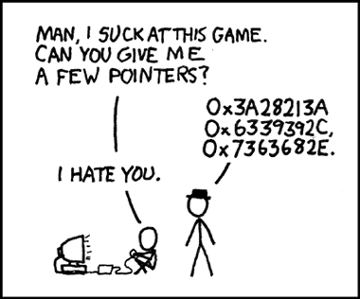
\includegraphics[keepaspectratio,width=0.6\textwidth]{elements/images/pointers.png}\par
  \vspace{5pt}
  \tiny{BY-NC 2.5 xkcd.com}
\end{center}
\par
\vspace{10pt}
\vfill
\newpage
\visa{UTI VÅR HAGE}
\vspace{10pt}
Uti vår hage där växa blåbär.\\
Kom hjärtans fröjd!\\
Vill du mig något, så träffas vi där.\\
Kom liljor och akvileja,\\
kom rosor och salivia,\\
kom ljuva krusmynta, kom hjärtans fröjd!\\
\\
Fagra små blommor där bjuda till dans.\\
Kom hjärtans fröjd!\\
Vill du så binder jag åt dig en krans.\\
Kom liljor...\\
\\
Kransen den sätter jag sen i ditt hår.\\
Kom hjärtans fröjd!\\
Solen den dalar, men hoppet uppgår.\\
Kom liljor...\\
\\
Uti vår hage finns blommor och bär.\\
Kom hjärtans fröjd!\\
Men utav alla du kärast mig är.\\
Kom liljor...
\par
\vspace{10pt}
{\footnotesize\textit{Folkvisa från Gotland.}}

\newpage
\fvisa{ÄNGLMARK}{Kalla den änglamarken eller himlajorden om du vill}
\vspace{10pt}
Kalla den änglamarken eller himlajorden om du vill,\\
jorden vi ärvde och lunden den gröna,\\
vildrosor och blåsippor och lindblommor och kamomill\\
låt dem få leva, de är ju så sköna!\par
\vspace{10pt}
Låt barnen dansa som änglar kring lönn och alm,\\
leka tittut mellan blommande grenar,\\
låt fåglar leva och sjunga för oss sin psalm\\
låt fiskar simma kring bryggor och stenar.\par
\vspace{10pt}
Sluta att utrota skogarnas alla djur.\\
Låt örnen flyga, låt rådjuren löpa!\\
Låt sista älven som brusar i vår natur\\
brusa alltjämt mellan fjällar och gran och fur.\par
\vspace{10pt}
Kalla den änglamarken eller himlajorden om du vill,\\
jorden vi ärvde och lunden den gröna,\\
vildrosor och blåsippor och lindblommor och kamomill\\
låt dem få leva, de är ju så sköna!\par
\vspace{10pt}
{\footnotesize\textit{Text \& Musik: Evert Taube}}

\newpage
\fvisa{ÖPPNA LANDSKAP}{Jag trivs bäst i öppna landskap}
\vspace{10pt}
Jag trivs bäst i öppna landskap\\
nära havet vill jag bo\\
några månader om året\\
så att själen kan få ro.\\
Jag trivs bäst i öppna landskap\\
där vindarna får fart.\\
Där lärkorna slår högt i skyn\\
och sjunger underbart.\\
Där bränner jag mitt brännvin själv\\
och kryddar med Johannesört\\
och dricker det med välbehag\\
till sill och hembakt vört.\\
Jag trivs bäst i öppna landskap\\
nära havet vill jag bo.\\
\\
Jag trivs bäst i fred och frihet\\
för både kropp och själ\\
ingen kommer in i min närhet\\
som stänger in och stjäl.\\
Jag trivs bäst när dagen bräcker\\
d'r fälten fylls av ljus\\
när tuppar gal på avstånd\\
när det är långt till närmsta hus.\\
Men ändå så pass nära\\
att en tyst och stilla natt\\
när man sitter under stjärnorna\\
kan höra festens skratt.\\
Jag trivs bäst i fred och frihet\\
för både kropp och själ.\\
\\
Jag trivs bäst när havet svallar\\
och måsarna ger skri\\
när stranden fylls med snäckskal\\
med havsmusik uti.\\
När det klara och det enkla\\
får råda som det vill\\
när ja är ja och nej är nej\\
och tvivlet tiger still.\\
Då binder jag en krans av löv\\
och lägger den vid närmasta sten\\
där runor ristats för vår skull\\
nån gång för länge sen.\\
Jag trivs bäst när havet svallar\\
och måsarna ger skri.\\
\vspace{10pt}
{\footnotesize\textit{Text \& Musik: Ulf Lundell}}

\newpage
\fvisa{JAMTLANDSSÅNGEN}{Ma går på stigom}
{\footnotesize\textit{Melodi: Jämtlandssången}}\\
\\
Ma går på stigom\\
å leit oss opp öve backan,\\
bort milla åkrom opp hitat vållom,\\
der bjällan pingel skvällt\\
i jänsmässti.\\
\\
Ma sir frå höjdom\\
bort mot åsom,\\
der kjörsan står milla gålom\\
bort ditat fjällom vår\\
der Skuta står,\\
så gnistrenes vit.\\
\\
\revrpt Fejen så sjong ma att JAMTLAND DE E LANNE\\
VÅRT!\\
I tusen år ha ma hadd’e,\\
håll’e därför hårt.\\
Ler ta den friheit som fedran ein gång at oss ga!\\
Hen ske ma lava å minnes allt,\\
som fedran oss sa.\rpt\\
\\
{\footnotesize\textit{Text: P-G Norman/Bo Oscarsson}}

\newpage
\visa{LÅNGT NER I SMÅLAND}
\vspace{10pt}
Långt ner i Småland,\\
där rider själva djävulen\\
med laddade pistoler och knallande gevär,\\
och alla små djävlar, dom spelar på fioler,\\
och själva fader Satan, han spelar handklaver.\par
\vspace{10pt}
Hurra för Svealand,\\
hurra för Götaland,\\
hurra för potatisland\\
som ger oss brännevin.\par
\vspace{10pt}
Ja, nog har vi glas,\\
men vi haver inget brännevin.\\
Finnes någon handlingsman\\
som haver ett glas öl.\par
\vspace{10pt}
Hurra för Svealand...\par
\vspace{10pt}
Ja, nubben kan tagas\\
på mångahanda sätt och vis.\\
Den lindar sig kring hjärtat\\
som rumpan på en gris.\par
\vspace{10pt}
Hurra för Svealand...

\newpage
\fvisa{Internationalen}{Upp trälar uti alla stater}\par
\vspace{10pt}
Upp, trälar uti alla stater,\\
som hungern bojor lagt uppå\\
Det dånar uti rättens krater,\\
snart skall uppbrottets timma slå.\\
Störtas skall det gamla snart i gruset.\\
Slav, stig upp för att slå dig fri!\\
Från mörkret stiga vi mot ljuset,\\
från intet allt vi vilja bli.\par
\vspace{10pt}
Upp till kamp emot kvalen.\\
Siste striden det är,\\
ty Internationalen\\
till alla lycka bär.\\
Upp till kamp emot kvalen.\\
Sista striden det är,\\
ty Internationalen\\
åt alla lycka bär.\par
\vspace{10pt}
I höjden räddarn vi ej hälsa,\\
ej gudar, furstar stå oss bi,\\
nej, själva vilja vi oss frälsa,\\
och samfälld skall vår räddning bli\\
För att kräva ut det stulna, bröder,\\
och för att slita andens band,\\
vi smida medan järnet glöder,\\
med senig arm och kraftig hand.\par
\vspace{10pt}
Upp till kamp emot kvalen...\par
\newpage
I sin förgudning avskyvärda,\\
månn'guldets kungar nånsin haft\\
ett annat mål än att bli närda\\
av proletärens arbetskraft?\\
Vad han skapat under nöd och vaka\\
utav tjuvar rånat är;\\
när folket kräva det tillbaka\\
sin egen rätt de blott begär.\par
\vspace{10pt}
I sin förgudning avskyvärda,\\
Upp till kamp emot kvalen...\par
\vspace{10pt}
I sin förgudning avskyvärda,\\
Båd'stat och lagar oss förtrycka\\
vi under skatter dignar ner.\\
Den rike inga plikter tycka,\\
den arme ingen rätt man ger.\\
Länge nog som myndingar vi böjt oss,\\
jämlikheten skall nu bli lag.\\
Med plikterna vi hittills nöjt oss .\\
Nu taga vi vår rätt en dag.\par
\vspace{10pt}
Upp till kamp emot kvalen...\par
\vfill
\hfill {\footnotesize\textit{forts. $\rightarrow$}}
\newpage
Till krigets slaktande vi dragits,\\
vi mejats ned i jämna led.\\
För furstars lögner har vi slagits,\\
nu vill vi skapa evig fred.\\
Om de oss driver, dessa kanibaler,\\
mot våra grannar än en gång,\\
vi skjuter våra generaler\\
och sjunger broderskapets sång.\par
\vspace{10pt}
Upp till kamp emot kvalen...\par
\vspace{10pt}
Arbetare, i stad på landet,\\
en gång skall jorden bliva vår\\
När fast vi knyta brodersbandet,\\
då lättingen ej råda får.\\
Många rovdjur på vårt blod sig mätta\\
men när vi nu till vårt försvar,\\
en dag en gräns för dessa sätta,\\
skall solen stråla lika klar.\par
\vspace{10pt}
Upp till kamp emot kvalen...

\newpage
\visa{Jungman Jansson}
\vspace{10pt}
Hej å hå jungman Jansson, redan friskar morgonvinden,\\
sista natten rullat undan, och Constantia ska' gå.\\
Har du gråtit med din Stina, har du kysst din mor på kinden,\\
har du druckit ur ditt brännvin så sjung hej å hå!\par
\vspace{10pt}
Hej å hå, jungman Jansson, är du rädd din lilla snärta\\
ska bedraga dej, bedraga dej och för en annan slå?\\
Och som morgonstjärnor blinka, säj, så bultar väl ditt hjärta,\\
vänd din näsa rätt mot stormen och sjung hej å hå!\par
\vspace{10pt}
Hej å hå, jungman Jansson, kanske ödeslotten faller,\\
ej bland kvinnfolk, men bland hajarna i Söderhaven blå?\\
Kanske döden står och lurar bakom trasiga koraller -\\
han är hårdhänt, men hederlig, så sjung hej å hå!\par
\vspace{10pt}
Kanske sitter du som gammal på en farm i Alabama,\\
medan åren siktas långsamt över tinningarna grå.\\
Kanske glömmer du din Stina för en sup i Jokohama -\\
det är slarvigt, med mänskligt, så sjung hej å hå!
\par
\vspace{10pt}
{\footnotesize\textit{Text och Musik: Dan Andersson}}

\newpage
\fvisa{KUNG LOUIE'S SÅNG}{Jag kungen är över alla här}
\vspace{10pt}
Jag kungen är över alla här\\
under trädens gröna höjd.\\
Jag har nått opp, till högsta topp,\\
men ännu är jag ej nöjd.\\
Jag vill bara va' en män'ska,\\
och kunna allt Ni kan.\\
Jag vill inte längre apa mig,\\
jag vill bara va en man.\par
\vspace{10pt}
Oh, obido. Jag vill va som du.\\
Jag vill se ut som du, gå som du, du.\\
Det vill jag nu, ett djur som jag.\\
Det lär sig bra bli en människa.\par
\vspace{10pt}
Försök inte lura mig gosse,\\
jag inga konster tål.\\
Att känna till hur eld blir till,\\
det är mina drömmars mål.\\
Din hemlighet vill jag veta,\\
så säg hur det går till.\\
O' då blir jag visst en man till sist,\\
o' det är vad jag vill.\par
\vspace{10pt}
Oh, obido...\\
...Vill lära mig bli en människa.
\par
\vspace{10pt}
{\footnotesize\textit{Text: M. Söderhjälm\\Ur djungelboken}}

\newpage
\null
\vfill
\index{Ã1337: Part 4b@1337: Part 4b}
\vspace*{-10pt}
\begin{center}
  \label{13374b}
  \tiny{1337: Part 4b}\par
  \vspace{5pt}
  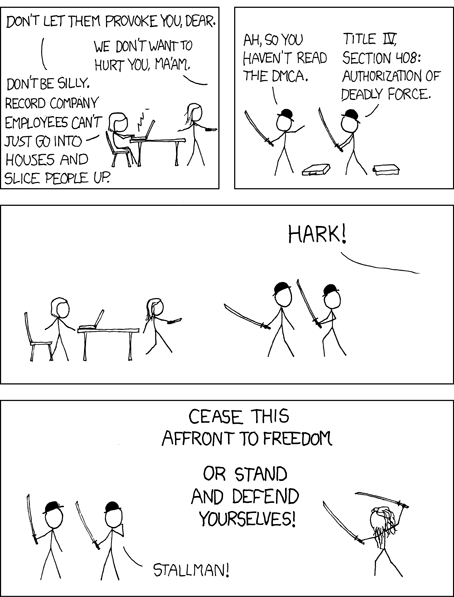
\includegraphics[keepaspectratio,width=0.8\textwidth]{elements/images/1337_part_4_2.png}\\
  \textline[t]{\tiny{\textit{s.\pageref{13374a} $\leftarrow$ föreg.}}}{\tiny{BY-NC 2.5 xkcd.com}}{\tiny{\textit{forts. $\rightarrow$ s.\pageref{13375a}}}}\par
\end{center}\par
\vspace*{-10pt}
\vfill
\null
\chapterpageimage{Osvenska visor}{Osvenska visor}{elements/osvenska.jpg}
\fvisa{ALWAYS LOOK ON THE BRIGHT SIDE SIDE OF LIFE}{Some things in life are bad}
\vspace{10pt}
Some things in life are bad\\
They can really make you mad\\
Other things just make you swear and curse.\\
When you're chewing on life's gristle\\
Don't grumble, give a whistle\\
And this'll help things turn out for the best...\par
\vspace{10pt}
And...always look on the bright side of life...\\
Always look on the light side of life...\par
\vspace{10pt}
If life seems jolly rotten\\
There's something you've forgotten\\
And that's to laugh and smile and dance and sing.\\
When you're feeling in the dumps\\
Don't be silly chumps\\
Just purse your lips and whistle - that's the thing.\par
\vspace{10pt}
And...\par
\vspace{10pt}
For life is quite absurd\\
And death's the final word\\
You must always face the curtain with a bow.\\
Forget about your sin - give the audience a grin\\
Enjoy it - it's your last chance anyhow.\par
\vspace{10pt}
And...\par
\newpage
Life's a piece of shit\\
When you look at it\\
Life's a laugh and death's a joke, it's true.\\
You'll see it's all a show\\
Keep 'em laughing as you go\\
Just remember that the last laugh is on you.\par
\vspace{10pt}
And...\par
\vspace{10pt}
{\footnotesize\textit{Text \& Musik: Eric Idle \\ Ur Life of Brian}}

\vspace{15pt}
\visa{Sit on my face}
\vspace{10pt}
Sit on my face and tell me that you love me\\
I'll sit on your face and tell you I love you too\\
I love to hear you oralize\\
When I'm between your thighs\\
You blow me away\par
\vspace{10pt}
Sit on my face and let my lips embrace you\\
I'll sit on your face and then I'll love you truly\\
Life can be fine if we both sixty nine\\
If we sit on our faces in all sorts of places\\
And play till we're blown away
\par
\vspace{10pt}
{\footnotesize\textit{Text: Eric Idle \& Harry Parr-Davies\\
Från Monty Python's Contractual Obligation Album.}}

\newpage
\fvisa{PROUD MARY}{Left a good job in the city}
\vspace{10pt}
Left a good job in the city,\\
working for the Man ev'ry night and day,\\
and I never lost one minute of sleepin',\\
worryin' 'bout the way things might have been.\par
\vspace{10pt}
Big wheel keep on turnin',\\
Proud Mary keep on burnin',\\
rollin' rollin' rollin' on the river.\par
\vspace{10pt}
Cleaned a lot of plates in Memphis,\\
pumped a lot of pain down in New Orleans,\\
but I never saw the good side of the city,\\
'til I hitched a ride on a riverboat queen\par
\vspace{10pt}
Big wheel, keep on turnin...\par
\vspace{10pt}
If you come down to the river,\\
bet you gonna find some people who live.\\
You don't have to worry 'cause you have no money,\\
people on the river are happy to give.\par
\vspace{10pt}
Big wheel, keep on turnin...\\
Rollin' rollin' rollin' on the river.
\par
\vspace{10pt}
{\footnotesize\textit{Text \& Musik: John Fogerty}}

\newpage
\fvisa{MÅ SAFTEN VARA MED ER}{Tell me Master Yoda, what is wrong with me?}
{\footnotesize\textit{Melodi: Obla-di obla-da}}\par
\vspace{10pt}
Tell me Master Yoda, what is wrong with me?\\
Feels like I've been stepped on by a horse.\\
Could it be that I have drunk a galaxy\\
and underestimate the dark side of the Force?\par
\vspace{10pt}
Obi-Wan, Obi two, Obi three,\\
hit me with your laser drink.\\
Obi-Wan, Obi two, come and save me! \\
Down under the bar I sink.\par
\vspace{10pt}
Waking up next morning was a big ordeal,\\
thought I had a Leia in my bed,\\
but you can imagine, Master, how i feel\\
when I see Jabba lying there with me instead.\par
\vspace{10pt}
Obi-Wan, Obi two, Obi three,\\
warp me to another place.\\
Obi-Wan, Obi two, come and save me!\\
Throwing up in hyperspace.\par
\vspace{10pt}
Calm down now, young Skywalker, you will be fine,\\
R2D2 would have laughed at this.\\
Help me drink this bottle of Han Solo’s wine\\
and I will tell you who your mother really is.\par
\vspace{10pt}
Obi-Wan, Obi two, Obi three,\\
drink and you will fly alright\\
Obi-Wan, Obi two, come and save me!\\
Man, I had a Jedi night!


\vspace*{-10pt}
\newpage
\fvisa{BLOWIN' IN THE WIND}{How many roads must a man walk down}
\vspace{10pt}
How many roads must a man walk down\\
Before you call him a man?\\
How many seas must a white dove sail\\
Before she sleeps in the sand?\\
Yes, how many times must the cannon balls fly\\
Before they're forever banned?\\
The answer my friend is blowin' in the wind\\
The answer is blowin' in the wind.\par
\vspace{10pt}
Yes, how many years can a mountain exist\\
Before it's washed to the sea?\\
Yes, how many years can some people exist\\
Before they're allowed to be free?\\
Yes, how many times can a man turn his head\\
Pretending he just doesn't see?\\
The answer my friend is blowin' in the wind\\
The answer is blowin' in the wind.\par
\vspace{10pt}
Yes, how many times must a man look up\\
Before he can see the sky?\\
Yes, how many ears must one man have\\
Before he can hear people cry?\\
Yes, how many deaths will it take till he knows\\
That too many people have died?\\
The answer my friend is blowin' in the wind\\
The answer is blowin' in the wind.\par
\vspace{10pt}
{\footnotesize\textit{Text: Bob Dylan}}

\newpage
\fvisa{THE ROSE}{Some say love it is a river}
\vspace{10pt}
Some say love it is a river\\
that drowns the tender reed.\\
Some say love it is a razor\\
that leaves your heart to bleed.\par
\vspace{10pt}
Some say love it is a hunger\\
an endless aching need.\\
I say love it is a flower\\
and you its only seed.\par
\vspace{10pt}
Its the heart afraid of breaking\\
that never learns to dance.\\
Its the dream afraid of waking\\
that never takes the chance.\par
\vspace{10pt}
It's the one who won't be taken\\
who can not seem to give.\\
And the soul afraid of dying\\
that never learns to live.\par
\vspace{10pt}
When the night has been too lonely\\
and the road has been too long.\\
And you think that love is only\\
for the lucky and the strong.\par
\vspace{10pt}
Just remember in the winter\\
far beneath the bitter snow,\\
lies the seed that with the sun's love\\
in the spring becomes the rose.
\par
\vspace{10pt}
{\footnotesize\textit{Text \& Musik: Amanda McBrown}}

\vspace*{-10pt}
\newpage
\visa{YESTERDAY}
\vspace{10pt}
Yesterday, all my troubles seemed so far away.\\
Now it look as though they're here to stay.\\
Oh, I believe in yesterday.\\
\\
Suddenly, I'm not half the man I used to be.\\
There's a shadow hanging over me.\\
Oh, yesterday came suddenly.\\
\\
Why she had to go I don't know, she wouldn't say.\\
I said something wrong, now I long for yesterday.\\
\\
Yesterday, love was such an easy game to play.\\
Now I need a place to hide away.\\
Oh, I believe in yesterday.\par
\vspace{10pt}
{\footnotesize\textit{Text \& Musik: Paul McCartney}}

\vspace{15pt}
\fvisa{BRIGHT EYES}{Is it a kind of dream}
\vspace{10pt}
Is it a kind of dream,\\
Floating out on the tide,\\
Following the river of death downstream?\\
Oh, is it a dream?\\
\\
There's a fog along the horizon,\\
A strange glow in the sky,\\
And nobody seems to know where you go,\\
And what does it mean?\\
Oh, is it a dream?\\
\\
Bright eyes,\\
Burning like fire.\\
Bright eyes,\\
How can you close and fail?\\
How can the light that burned so brightly\\
Suddenly burn so pale?\\
Bright eyes.\\
\\
Is it a kind of shadow,\\
Reaching into the night,\\
Wandering over the hills unseen,\\
Or is it a dream?\\
\\
There's a high wind in the trees,\\
A cold sound in the air,\\
And nobody ever knows when you go,\\
And where do you start,\\
Oh, into the dark.\\
\\
Bright eyes,\\
burning like fire.\\
Bright eyes,\\
how can you close and fail?\\
How can the light that burned so brightly\\
Suddenly burn so pale?\\
Bright eyes.\\
\\
Bright eyes,\\
burning like fire.\\
Bright eyes,\\
how can you close and fail?\\
How can the light that burned so brightly\\
Suddenly burn so pale?\\
Bright eyes.
\vspace{10pt}
{\footnotesize\textit{Text: Simon and Garfunkel}}

\newpage
\visa{WHEN WE GET DRUNKER}
{\footnotesize\textit{Melodi: When I'm sixty-four}}\par
\vspace{10pt}
When we get drunker, loosing our minds,\\
many beers from now.\\
Will we still be having us a real good time,\\
whiskey, gin and bottles of wine?\\
So fill up your glass now, get drunk as a skunk,\\
don't say you want no more.\\
We are the singers, we are the swingers\\
join us, you won't get bored!

\vspace{15pt}
\fvisa{DE BREVITATE VITAE}{Gaudeamus igitur}
\vspace{10pt}
Gaudeamus igitur\\
Juvenes dum sumus.\\
Gaudeamus igitur\\
Juvenes dum sumus.\\
Post jucundam juventutem\\
Post molestam senectutem\\
Nos habebit humus.\\
Nos habebit humus.\par
\vspace{10pt}
Vita nostra brevis est\\
Brevi finietur.\\
Vita nostra brevis est\\
Brevi finietur.\\
Venit mors velociter\\
Rapit nos atrociter\\
Nemini parcetur.\\
Nemini parcetur.\par
\newpage
Vivant omnes virgines\\
Faciles, formosae.\\
Vivant omnes virgines\\
Faciles, formosae.\\
Vivant et mulieres\\
Tenerae amabiles\\
Bonae laboriosae.\\
Bonae laboriosae.\par
\vspace{10pt}
Vivat academia!\\
Vivant professores!\\
Vivat academia!\\
Vivant professores!\\
Vivat membrum quodlibet\\
Vivant membra quaelibet\\
Semper sint in flore.\\
Semper sint in flore.\par
\vspace{10pt}
{\footnotesize\textit{Published by Halle in 1781 in Studentenlieder (``Students' Songs'') and written by Christian Wilhelm Kindleben (1748-1785)}}

\newpage
\fvisa{I Will Derive}{At first I was afraid}
{\footnotesize\textit{Melodi: I Will Survive}}\par
\vspace{10pt}
At first I was afraid, what could the answer be?\\
It said given this position find velocity.\\
So I tried to work it out,\\
but I knew that I was wrong.\\
I struggled; I cried,\\
``A problem shouldn't take this long!''\\
I tried to think, control my nerve.\\
It's evident that speed's tangential,\\
to that time-position curve.\\
This problem would be mine,\\
if I just knew that tangent line.\\
But what to do? Show me a sign!\par
\vspace{7pt}
So I thought back to Calculus.\\
Way back to Newton and to Leibniz,\\
And to problems just like this.\\
And just like that when I had given up all hope,\\
I said nope, there's just one way to find that slope.\\
And so now I, I will derive.\\
Find the derivative of x position with respect to time.\\
It's as easy as can be, just have to take dx/dt.\\
I will derive, I will derive. Hey, hey!\par
\newpage
And then I went ahead to the second part.\\
But as I looked at it I wasn't sure quite how to start.\\
It was asking for the time at which velocity\\
Was at a maximum, and I was thinking ``Woe is me.''\\
But then I thought, this much I know.\\
I've gotta find acceleration, set it equal to zero.\\
Now if I only knew what the function was for a.\\
I guess I'm gonna have to solve for it someway.\par
\vspace{10pt}
So I thought back to Calculus.\\
Way back to Newton and to Leibniz,\\
And to problems just like this.\\
And just like that when I had given up all hope,\\
I said nope, there's just one way to find that slope.\\
And so now I, I will derive.\\
Find the derivative of velocity with respect to time.\\
It's as easy as can be, just have to take dv/dt.\\
I will derive, I will derive.\par
\vspace{10pt}
So I thought back to Calculus.\\
Way back to Newton and to Leibniz,\\
And to problems just like this.\\
And just like that when I had given up all hope,\\
I said nope, there's just one way to find that slope.\\
And so now I, I will derive.\\
Find the derivative of x position with respect to time.\\
It's as easy as can be, just have to take dx/dt.\\
I will derive, I will derive, I will derive!

\newpage
\fvisa{LUMBERJACK SONG}{I'm a lumberjack}
\vspace{10pt}
\textbf{
I'm a lumberjack\\
And I'm O.K\\
I sleep all night\\
And I work all day\\
}
\\
He's a lumberjack\\
And he's O.K\\
He sleeps all night\\
And he works all day\par
\vspace{10pt}
\textbf{
I cut down trees'\\
I eat my lunch\\
I go to the lavatory\\
On Wednesdays I go shopping\\
And have buttered scones for tea\\
}
\\
He cuts down trees\\
He eats his lunch\\
He goes to the lavatory\\
On Wednesdays he goes shopping\\
And has buttered scones for tea\par
\vspace{10pt}
He's a lumberjack...\par
\vspace{10pt}
\textbf{
I cut down trees\\
I skip and jump\\
I like to press wild flowers\\
I put on women's clothing\\
And hang around in bars\\
}
\\
He cuts down trees\\
He skips and jumps\\
He likes to press wild flowers\\
He puts on women's clothing\\
And hangs around in bars\par
\vspace{10pt}
He's a lumberjack...\par
\vspace{10pt}
\textbf{
I cut down trees\\
I wear high heels\\
Suspenders and a bra\\
I wish I'd been a girlie\\
Just like my dear mama.\\
}
\\
He cuts down trees\\
He wears high heels\\
(sägs hellre än sjungs) Suspenders ..... and a bra?\\
That's shocking.\par
\vspace{10pt}
He's a lumberjack...
\par
\vspace{10pt}
{\footnotesize\textit{Text: Terry Jones \& Michael Palin}}

\newpage
\fvisa{Roma}{Jag satt en kväll i Roma}
{\footnotesize\textit{Melodi: Manschettvisan}}\par
\vspace{10pt}
Jag satt en kväll i Roma\\
och njöt cigarr aroma,\\
mitt fagra fysionoma\\
mot mången kvinna le.\par
\vspace{10pt}
Då kom en brallisita\\
med former trés bonita.\\
Ej utan all invita\\
var hennes bystament.\par
\vspace{10pt}
Hon sa på Roma måle:\\
``Ni vara fagro tvåle:\\
Jag har förslag frivole.\\
Vi älska med varann''.\par
\vspace{10pt}
Mitt inne bland spaljene\\
hon visa molto bene.\\
Mitt inne ibland grene\\
vi hade téte à téte.\par
\vspace{10pt}
Vi téte lite granda,\\
jag göra observanda\\
att kvinna confirmanda\\
hon vara långt ifrån.\par
\vspace{10pt}
Jag klänga kors och tvärso.\\
Det var en riktig pärzo.\\
Till sist bli kall om stjärtzo\\
och vi gå hem till hon.\par
\vspace{10pt}
Jag kysste'na mitt i nia.\\
Hon ropa: ``Madre mia!\\
Ni vara kyssgeni, ja''.\\
Jag släckte armatur.\par
\vspace{10pt}
Då kom där en señore\\
och skrek i hög tenore:\\
``Ni kan be Fadre Våre,\\
ty jag är hennes man''.\par
\vspace{10pt}
Han gjorde sig beretto\\
och drog en jädrans lång stiletto.\\
Jag kavla upp manschetto,\\
drog fram min nagelfil.\par
\vspace{10pt}
Så började duello\\
om denna bonne mamsello.\\
I hans akterkastello\\
jag rände mitt instrument.\par
\vspace{10pt}
Han vred sig i spirale\\
och ropade: ``Tvi vale'',\\
och la sig horisontale\\
och sluta sina dar.\par
\vspace{10pt}
Nu ligger han i jordo,\\
begravd av fattigvårdo,\\
och jag blev fast för mordo\\
och slängd i finkament.\par
\vspace{10pt}
Nu sitter jag i cello\\
och fäller många mjällo\\
för denna bonne mamsello,\\
ty hon hörs aldrig av.

\vspace*{-10pt}
\newpage
\visa{Roxanne}
{\footnotesize\textit{Melodi: Roxanne}}\par
\vspace{10pt}
Roxanne\\
You don't have to put on the red light\\
Those days are over\\
You don't have to sell your body to the night\\
Roxanne\\
You don't have to wear that dress tonight\\
Walk the streets for money\\
You don't care if it's wrong or if it's right\\
\\
Roxanne\\
You don't have to put on the red light\\
Roxanne\\
You don't have to put on the red light\\
\\
Roxanne put on the red light\\
Roxanne put on the red light\\
Roxanne put on the red light\\
Roxanne put on the red light\\
Roxanne put on the red light\\
\\
I loved you since I knew you\\
I wouldn't talk down to you\\
I have to tell you just how I feel\\
I won't share you with another boy\\
I know my mind is made up\\
So put away your makeup\\
Told you once I won't tell you again\\
It's a bad way\\
\\
Roxanne\\
You don't have to put on the red light\\
Roxanne\\
You don't have to put on the red light\\
\\
You don't have to put on the red light\\
Roxanne put on the red light\\
Roxanne put on the red light\\
Roxanne put on the red light\\
Roxanne put on the red light\\
Roxanne put on the red light\\
Roxanne put on the red light\\
Roxanne put on the red light\\
Roxanne put on the red light\\
Roxanne put on the red light\\
You don't have to put on the red light\\
Roxanne put on the red light\\
You don't have to put on the red light\\
Roxanne put on the red light\\
Roxanne put on the red light\\
Roxanne put on the red light
\par
\vspace{10pt}
{\footnotesize\textit{Text: The Police\\ Dryckesspel: ena gruppen dricker på roxanne och andra på red light}}

\newpage
\visa{SHE'LL BE COMING 'ROUND THE MOUNTAIN}
\vspace{10pt}
She'll be coming 'round the mountain when she comes.\\
She'll be coming 'round the mountain when she comes.\\
She'll be coming 'round the mountain,\\
She'll be coming 'round the mountain,\\
She'll be coming 'round the mountain when she comes.\par
\vspace{10pt}
Singing ay, ay, yippee, yippee, ay...\par
\vspace{10pt}
She'll be drinking all the whiskey when she comes...\par
\vspace{10pt}
She was wearing pink pyjamas when she came...\par
\vspace{10pt}
She was wearing no pyjamas making love...\par
\vspace{10pt}
She was wearing my pyjamas when she left...\par
\vspace{10pt}
She will never, never be the same again...

\vspace*{15pt}
\visa{Sancta lucia}
{\footnotesize\textit{Melodi: Sankta Lucia}}\par
\vspace{10pt}
Jag in silentio\\
gör promenado\\
nocturno solo\\
in Esplanado.\\
Jag där med grand favor\\
väntar min pia\\
Sancta Lucia, Sancta Lucia.\par
\newpage
Con vehementio\\
slår jag rivale\\
och etablerar\\
grande scandale.\\
Polisconstabelo\\
otti in krago\\
Sancta Lucia, Sancta Lucia.\par
\vspace{10pt}
Jag skrek fortissimo:\\
``Släpp mig för Phano!''\\
Han röt crescendo:\\
``Parla non guano!''\\
Jag in arresto förs\\
oh, infamia\\
Sancta Lucia, Sancta Lucia.\par
\vspace{10pt}
Oh, hårda destiné\\
här in obscuro\\
gråter jag lacrimae\\
ödet är duro.\\
Önskar al diavolo\\
amore mia\\
Satans Lucia, Satans Lucia.

\newpage
\visa{TRINK, TRINK, BRÜDERLEIN TRINK}
\vspace{10pt}
Trink, trink, Brüderlein, trink,\\
lass doch die Sorgen zu Haus!\\
Trink, trink, Brüderlein, trink,\\
zieh doch die Stirn nicht so krauss!\\
Meide den Kummer und meide den Schmerz,\\
dann ist das Leben ein Scherz!\\
Meide den Kummer und meide den Schmerz,\\
dann ist das Leben ein Scherz!\par
\vspace{10pt}
Das Trinken, das soll man nicht lassen,\\
das Trinken regiert doch die Welt,\\
man soll auch den Menschen nicht hassen,\\
der stets eine Lage bestellt.\\
Ob Bier, ob Wein, ob Champagner,\\
nur lasst uns beim Trinken nicht prahl'n,\\
es trank den Champagner schon mancher\\
und konnt ihn nachher nicht bezahl'n.\par
\vspace{10pt}
Trink, trink, Brüderlein, trink...\par
\vspace{10pt}
Das Lieben, das Trinken, das Singen\\
schafft Freude und fröhlichen Mut,\\
den Frauen, den musst du eins bringen,\\
sie sind doch so lieb und so gut.\\
Verlieb dich, solange du jung bist,\\
die Hauptsach', du bist noch nicht blau,\\
denn wenn man beim fröhlichen Trunk ist,\\
bekommt man sehr leicht eine Frau.\par
\vspace{10pt}
Trink, trink, Brüderlein, trink...\par
\vspace{10pt}
Der Moses, der hat, gar nicht übel,\\
ein elftes Gebot noch erdacht,\\
das steht aber nicht in der Bibel\\
und hat so viel Freude gemacht.\\
Man hatte es uns unterschlagen,\\
weil fröhliches Trinken es preist,\\
ich aber, ich will es euch sagen.\\
Ja, wisst ihr denn auch, wie es heisst?\par
\vspace{10pt}
Trink, trink, Brüderlein, trink...

\vspace{15pt}
\fvisa{Små grodorna (Latin)}{Ranunculi ranunculi}
\vspace{10pt}
Ranunculi ranunculi\\
Quam sunt ridiculi\\
\\
Ranunculi ranunculi\\
Quam sunt ridiculi\\
\\
Non aures, non aures\\
non caudas habent hi.\\
\\
Non aures, non aures\\
non caudas habent hi.

\newpage
\fvisa{Auld Lang Syne}{Should auld acquaintance be forgot}
{\footnotesize\textit{Melodi: Skotskt Traditionell}}\par
\vspace{10pt}
Should auld acquaintance be forgot,\\
and never brought to mind?\\
Should auld acquaintance be forgot,\\
and auld lang syne?\par
\vspace{10pt}
For auld lang syne, my jo,\\
for auld lang syne,\\
we'll tak' a cup o' kindness yet,\\
for auld lang syne.\par
\vspace{10pt}
And surely ye'll be your pint-stoup!\\
and surely I'll be mine!\\
And we'll tak' a cup o' kindness yet,\\
for auld lang syne.\par
\vspace{10pt}
For auld lang syne, my jo...\par
\vspace{10pt}
We twa hae run about the braes,\\
and pou'd the gowans fine;\\
But we've wander'd mony a weary fit,\\
sin' auld lang syne.\par
\vspace{10pt}
For auld lang syne, my jo...\par
\vspace{10pt}
We twa hae paidl'd in the burn,\\
frae morning sun till dine;\\
But seas between us braid hae roar'd\\
sin' auld lang syne.\par
\newpage
For auld lang syne, my jo...\par
\vspace{10pt}
And there's a hand, my trusty fiere!\\
and gie's a hand o' thine!\\
And we'll tak' a right gude-willie waught,\\
for auld lang syne.\par
\vspace{10pt}
For auld lang syne, my jo...\par
\vspace{15pt}
{\footnotesize\textit{``Scots pronunciation guide'' finnes på nästa uppslag. $\rightarrow$}}\par
\newpage
\svisa{Auld Lang Syne - Scots pronunciation guide}{Shid ald akwentans bee firgot}{Auld Lang Syne - \\Scots pronunciation guide}
{\footnotesize\textit{Melodi: Skotskt Traditionell}}\par
\vspace{10pt}
Shid ald akwentans bee firgot,\\
an nivir brocht ti mynd?\\
Shid ald akwentans bee firgot,\\
an ald lang syn?\par
\vspace{9pt}
Fir ald lang syn, ma jo,\\
fir ald lang syn,\\
wil tak a cup o kyndnes yet,\\
fir ald lang syn.\par
\vspace{9pt}
An sheerly yil bee yur pynt-staup!\\
an sheerly al bee myn!\\
An will tak a cup o kyndnes yet,\\
fir ald lang syn.\par
\vspace{9pt}
Fir ald lang syn, ma jo...\par
\vspace{9pt}
We twa hay rin aboot the braes,\\
an pood the gowans fyn;\\
Bit weev wandert monae a weery fet,\\
sin ald lang syn.\par
\vspace{9pt}
Fir ald lang syn, ma jo...\par
\vspace{9pt}
We twa hay pedilt in the burn,\\
fray mornin sun til dyn;\\
But seas between us bred hay roard\\
sin ald lang syn.\par
\newpage
Fir ald lang syn, ma jo...\par
\vspace{10pt}
An thers a han, my trustee feer!\\
an gees a han o thyn!\\
And we'll tak a richt gude-willie-waucht,\\
fir ald lang syn.\par
\vspace{10pt}
Fir ald lang syn, ma jo...

\vspace{15pt}
\visa{Professor Baltazar}
\vspace{10pt}
Balt, Balt, Baltazar.\\
Balt, Balt, Baltazar.\\
Baltazar\\
Baltazar\\
Baltazar.
\par
\vspace{10pt}
{\footnotesize\textit{Professor Balthazar är namnet på en animerad
TV-serie ifrån 1967 producerad av den kroatiska animationstudion
Zagreb Film och animatören Zlatko Grgić.}}

\newpage
\fvisa{THE LAUGHING POLICEMAN}{I know a fat old policeman}
\vspace{10pt}
(\textit{Laughter})\par
\vspace{10pt}
I know a fat old policeman\\
He's always on our street\\
A fat and jolly red-faced man\\
He really is a treat\par
\vspace{10pt}
He's too kind for a policeman\\
He's never known to frown\\
And everybody says\\
He is the happiest man in town!\par
\vspace{10pt}
(\textit{Laughter})\par
\vspace{10pt}
He laughs upon point duty\\
He laughs upon his beat\\
He laughs at everybody\\
When he's walking in the street\par
\vspace{10pt}
He never can stop laughing\\
He says he's never tried\\
But once he did arrest a man\\
And laughed until he cried!\par
\vspace{10pt}
(\textit{Laughter})\par
\vspace{10pt}
His jolly face is wrinkled\\
And then he shut his eyes\\
He opened his great big mouth\\
It was a wonderous size!\par
\vspace{10pt}
He said: ``I must arrest you!''\\
He didn't know what for\\
And then he started laughing\\
Until he cracked his jaw!\par
\vspace{10pt}
(\textit{Laughter})\par
\vspace{10pt}
So if you chance to meet him\\
While walking 'round the town\\
Shake him by his fat ol' hand\\
And give him half a crown\par
\vspace{10pt}
His eyes will beam and sparkle\\
He'll gurgle with delight\\
And then you'll start him laughing\\
With all his blessed might!

\newpage
\fvisa{OUR FAMILY}{My father makes counterfeit money}
{\footnotesize\textit{Melodi: My Bonnie}}
My father makes counterfeit money,\\
my mother makes synthetic gin.\\
My sister sells kisses to sailors,\\
and that's how the money rolls in'.\par
\vspace{10pt}
\revrpt Rolls in, rolls in,\\
thats how the money rolls in, rolls in' \rpt\par
\vspace{10pt}
My uncle's a slum missionary,\\
saving young maidens from sin.\\
He'll save you a blonde for a shilling,\\
and that's how the money rolls in'\par
\vspace{10pt}
Rolls in...\par
\vspace{10pt}
My aunt runs a girl's seminary,\\
teaching young girls to begin.\\
She doesn't say where they've to finish,\\
and that's how the money rolls in'.\par
\vspace{10pt}
Rolls in...\par
\vspace{10pt}
My father has spent all his money,\\
my mother has drunk all her gin.\\
My sister’s beauty has fainted,\\
and no more money rolls in!
\par
\vspace{10pt}

\newpage
\null
\vfill
\index{Ã1337: Part 5a@1337: Part 5a}
\vspace*{-10pt}
\begin{center}
  \label{13375a}
  \tiny{1337: Part 5a}\par
  \vspace{5pt}
  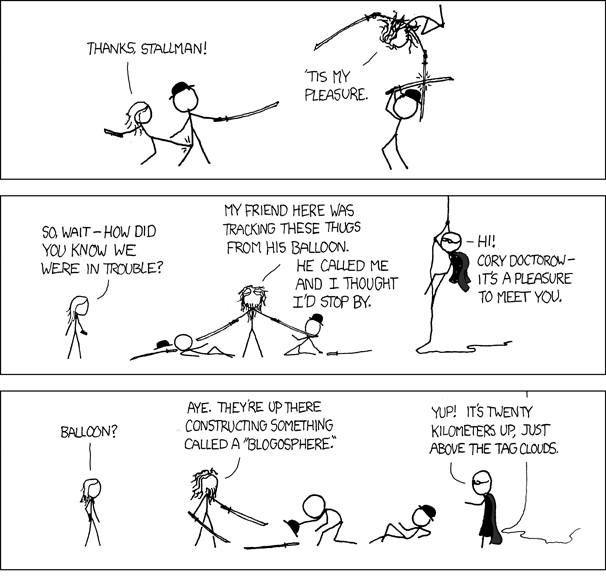
\includegraphics[keepaspectratio,width=0.9\textwidth]{elements/images/1337_part_5_1.png}\\
  \textline[t]{\tiny{\textit{s.\pageref{13374b} $\leftarrow$ föreg.}}}{\tiny{BY-NC 2.5 xkcd.com}}{\tiny{\textit{forts. $\rightarrow$ s.\pageref{13375b}}}}\par
\end{center}\par
\vfill
\null
\chapterpageimage{Interwebz}{Interwebz}{elements/interwebz.jpg}
\visa{ANSIKTSBURK}
{\footnotesize\textit{Melodi: Am Tekbar el Farha}}\par
\vspace{10pt}
Ansiktsburk, ansiktsburk\\
han fick vad han ville för hatt\\
Han tjalla' på sin lilla tjeeeej\\
tjohofidelittan, hatt\par
\vspace{10pt}
Ansiktsburk, ansiktsburk\\
han fick vad han ville för hatt\\
Han tjalla' på sin lilla tjeeeej\\
tjohofidelittan, hatt\par
\vspace{10pt}
Hammarby-Nisse är haaaarlig\\
Bitter e han ej - ja, jääääävligt\\
Hammarby-Nisse är haaaarlig\\
Bitter e han ej - jaha, jääääävligt\par
\vspace{10pt}
När hatten har blitt färdig\\
rasar han in för en ha-aaaaatt\par
\vspace{10pt}
Ansiktsburk, ansiktsburk\\
han fick vad han ville för hatt\\
Han tjalla' på sin lilla tjeeeej\\
tjohofidelittan, hatt

\newpage
\visa{I Can't Poop In Strange Places}
\vspace{10pt}
\par
I can't poop in strange places\\
(strange places)\\
I can only poop in my home\\
It's as though i'm watched by strange faces\\
(strange faces)\\
I'ts why I never roam\par
\vspace{10pt}
I've left Stewie alone with strangers\\
(strangers)\\
To satisfy my fecal needs\\
I've put my whole family in danger\\
To poop before my anus bleeds\par
\vspace{10pt}
Home bowl, home bowl\\
You know just what I need\\
Home bowl, home bowl\\
Poop before my anus bleeds\par
\vspace{10pt}
{\footnotesize\textit{Glenn Quagmire and Peter Griffin perform this amazing song}}

\newpage
\fvisa{Llama song}{Here's a llama}
\vspace{10pt}
Here's a llama, there's a llama, and another little Llama\\
Fuzzy Llama, Funny Llama, llama llama duck\\
\\
Llama, llama, cheesecake, llama, tablet, brick, potato llama, llama llama, mushroom llama, llama llama duck\\
\\
I was once a treehouse, i lived in a cake,\\
though i never saw the way, the orange slayed the rake,\\
i was only three years dead, but it told a tale\\
and now listen, little child, to the safety rail\\
\\
Have you ever seen a llama, kiss a llama, on a llama\\
llama's llama, tastes of llama, llama llama duck\\
\\
half a llama, twice a llama, not a llama, farmer llama\\
llama in a car, alarm a llama llama duck\\
\\
is it how it's told now? is it all so old?\\
is it made of lemon juice? doorknob, ankle, cold\\
now my song is getting thin, i've run out of luck!\\
time for me to retire now, and become a duck

\newpage
\fvisa{FANTASTIK HÄST}{Se på min häst, min häst är fantastisk}
{\footnotesize\textit{Melodi: Amazing Horse}}
\vspace{10pt}
Se på min häst, min häst är fantastisk\\
Ge den en slick!\par
\vspace{10pt}
Mmm, den smakar som russin!\par
\vspace{10pt}
När man stryker dess man, förvandlas den till ett plan,\\
och förvandlas igen när man drar i dess \textit{penis}\par
\vspace{10pt}
Åh, va snuskigt!\par
\vspace{10pt}
Tycker du det? Då borde jag nog inte\\
visa dig vad jag gör med min lemonad.\\
Söt lemonad, åh, söt lemonad,\\
söt lemonad, ja, söt lemonad!\par
\vspace{10pt}
...\par
\vspace{10pt}
Upp på min häst, vi flyger runt i rymden!\\
Och alla andra platser med!\par
\vspace{10pt}
Jag tror att du lär inse att vår rymd\\
i princip täcker nästan...\par
\vspace{10pt}
Käften \textit{kvinna}, upp på min häst!

\newpage
\fvisa{Parents are gross}{You never should look at your mother's boobies}
\vspace{10pt}
You never should look at your mother's boobies\\
No matter how big and round they are\\
You'll end up seeing something you don't wanna\\
It's guaranteed to leave a mental scar\\
You never should look at your daddy's penis\\
When he's walkin' down the hall on Sunday morn\\
An acorn in a nest of twigs\\
And underneath two fetal pigs\\
It'll make you wish you weren't even born\par
\vspace{10pt}
Parents are gross, parents are gross...
\par
\vspace{10pt}
{\footnotesize\textit{``Parents Are Gross'' is sung by Peter Griffin and Glenn Quagmire in ``In Harmony's Way'' on Conan O'Brien's show until Peter's antics cause Quagmire to storm offstage.}}

\newpage
\fvisa{The Duck Song}{A duck walked up to a lemonade stand}\index{Duck Song@The Duck Song}
\vspace{10pt}
(Bum bum bum, ba-dum ba-dum)\\
A duck walked up to a lemonade stand\\
And he said to the man, running the stand\\
``Hey! (Bum bum bum) Got any grapes?''\\
The man said\\
``No, we just sell lemonade. But it's cold\\
And it's fresh\\
And it's all home-made. Can I get you\\
glass?''\\
The duck said,\\
``I'll pass.''\par
\vspace{10pt}
Then he waddled away.\\
(Waddle waddle)\\
'Til the very next day.\\
(Bum bum bum bum Bum da-dum)\par
\vspace{10pt}
The duck walked up to the lemonade stand\\
And he said to the man, running the stand,\\
``Hey! (Bum bum bum) Got any grapes?''\\
The man said\\
``No, like I said yesterday,\\
We just sell lemonade. OK?\\
Why not give it a try?''\\
The duck said,\\
``Goodbye.''
\newpage
Then he waddled away.\\
(Waddle waddle)\\
Then he waddled away.\\
(Waddle waddle waddle)\\
Then he waddled away\\
(Waddle waddle)\\
'Til the very next day.\\
(Bum bum bum bum bum ba-dum)\par
\vspace{10pt}
When the duck walked up to the lemonade stand\\
And he said to the man running the stand,\\
``Hey! (bum bum bum) Got any grapes?''\\
The man said,\\
``Look, this is getting old.\\
I mean, lemonade's all we've ever sold.\\
Why not give it a go?''\\
The duck said,\\
``How 'bout, no.''\par
\vspace{10pt}
Then he waddled away\\
(Waddle waddle)\\
Then he waddled away.\\
(Waddle waddle waddle)\\
Then he waddled away\\
(Waddle waddle)\\
'Til the very next day.\\
(Bum bum bum bum bum ba-dum)\par
\vfill
\hfill {\footnotesize\textit{forts. $\rightarrow$}}
\newpage
When the duck walked up to the lemonade stand\\
And he said to the man running the stand,\\
``Hey! (Bum bum bum) Got any grapes?''\\
The man said,\\
``THAT’S IT!\\
If you don't stay away, Duck,\\
I'll glue you to a tree and leave you there all day,\\
stuck.\\
So don't get to close!''\\
The duck said,\\
``Adios.''\par
\vspace{10pt}
Then he waddled away.\\
(Waddle waddle)\\
Then he waddled away.\\
(Waddle waddle waddle)\\
Then he waddled away\\
(Waddle waddle)\\
'Til the very next day.\\
(Bum bum bum bum bum ba-dum)\par
\vspace{10pt}
When the duck walked up to the lemonade stand\\
And he said to the man running the stand,\\
``Hey! (Bum bum bum) got any glue?''\\
``What?''\\
``Got any glue?''\\
``No, why would I– oh!''\\
And one more question for you;\\
``Got any grapes?''\\
(Bum bum bum, bum bum bum)
\newpage
And the man just stopped.\\
Then he started to smile.\\
He started to laugh.\\
He laughed for a while.\\
He said,\\
``Come on duck, let’s walk to the store.\\
I’ll buy you some grapes\\
So you won't have to ask anymore.''\\
So they walked to the store\\
And the man bought some grapes.\\
He gave one to the duck and the duck said,\\
``Hmm... No thanks. But you know what sounds good?\\
It would make my day.\\
Do you think this store...\\
Do you think this store...\\
Do you think this store... has any... lemonade?''\par
\vspace{10pt}
(Fading)\\
Then he waddled away.\\
(Waddle waddle)\\
Then he waddled away.\\
(Waddle waddle waddle)\\
Then he waddled away\\
(Waddle waddle)

\newpage
\fvisa{Hatten är din}{Lalalalala}
\vspace{10pt}
Lalalala...\\
Åååååååhhh\\
Vinna kinky roligt, vinna kinky roligt\\
Hatten är din, hatten är din\\
Hatt-baby, hatt-baby\\
Den hatten lever så roligt,\\
den hatten lever så roligt\\
Hatten är din, hatten är din\\
Hatt-baby hatt-baby\\
Det här är förjävligt\\
Det tycker vi blir bögigt\\
Det alltid var roligt\\
Hatten är din ... 2ggr\\
Lalalalala\\
Åååååååhhh\\
\\
Cool kille med läsk I hand\\
Ja, det tycker vi - nånting sött\\
Cool kille med läsk I hand\\
Ja, det tycker vi - nånting sött\\
\revrpt Välte hatten i Berts cola-au-lait \rpt \\
\revrpt Men sen visste nog du, att baby \rpt \\
\revrpt Men sen visste nog du, hatt baby \rpt \\
Hatten är din ...\\
Lalalala\\
Åååååååhhh\\
\\
Låna LP:n "Hatten är din"\\
Man kan klä ut sej och hångla i TV\\
Lana LP:n "Hatten är din"\\
Man kan knarka och hamna i TV\\
\revrpt Hatten är visst det din, din!AAA \rpt \\
\revrpt Alla vet varför och allt blir perfekt \\
Alla vet varför och allt blir perfekt \rpt \\
Hatten är din ... \\
Lalalala\\
Åååååååhhh\\
\\
Limma skinkbit cooligt\\
Limma skinkbit cooligt, cooligt\\
Hatten är din ...\\
\revrpt Hatten lever så roligt \rpt \\
Ja, det hatten lever så roligt\\
Vi har det förjävligt\\
Det tycker vi blir bögigt\\
Det alltid var roligt\\
\revrpt Hatten är din ... \rpt \\
Lalalala\\
Lalalala
\newpage
\visa{Trololo}
{\footnotesize\textit{Melodi: Mr.Trololo}}\par
\vspace{10pt}
Ahhhhhhhhh\\
Ya ya yaaaah\\
Ya ya yaaah\\
Yaaah ya yah\\
\\
Ohohohohoooo\\
Oh ya yaaah\\
Ya ya yaaah\\
Yaaah ya yah\\
\\
Ye-ye-ye-ye-yeh\\
Ye-ye-yeh\\
Ye-ye-yeh\\
Ohohohohoh\\
\\
Ye-ye-ye-ye-yeh\\
Ye-ye-yeh\\
Ye-ye-yeh\\
Ohohohohooooooooooo\\
Aaaaoooooh aaaooo\\
Hooo haha\\
\\
Nah nah nah nah\\
Nuh nuh nuh\\
Nuh nuh nuh\\
Nuh nuh nuh\\
Nuh nuh nah!\\
\\
Nah nah nah nah nun\\
Nun-ah nun\\
Nun-ah nuh\\
Nah nah nah nah nah!\\
\\
Nah nah nah nah Naaaaaaaaaaaaaaaaaaaaaaaaah!\\
Dah dah daaaaaaaaaah...\\
Da-da-dah...\\
Daaah.\\
Da-dah...\\
\\
Trolololololoooooooooooooo!\\
\\
Lah la-laaah\\
La la laaah\\
lol\\
haha\\
\\
Ohohohoho\\
ho-ho-ho\\
ho-ho-ho\\
oh-ho-ho-ho-ho\\
\\
Ohohohoho\\
ho-ho-ho\\
ho-ho-ho\\
Lololololooo...\\
\\
AAIIEEEEEEEEEEEEEEEEEEEEEEEEEEEEEEEEEEEEEEEEEEEEEEEE\\
eeeee-eeeee-EEEEEEEEE!\\
\\
Luh-luh-lah...\\
Lah\\
Lah-lah\\
\\
Ohohohohooooooooo!\\
BOPadududu-dah-da-du-daaaah!\\
Da-da-daaaah\\
Daaah\\
Da-daaah...\\
\\
Trololololo\\
Trolololo\\
Trolololol\\
Lalalalah!\\
\\
Trolololo\\
lalala\\
\\
Oh-hahaha-ho\\
Haha-hehe-ho\\
Hohoho-he-ho\\
Hahahaha-ho\\
\\
Trolololololo\\
Trolololololo\\
Trolololololo\\
Lololo-LOL!\\
\\
Aaaaaaaaaaahhhhhhhhhhhhh!\\
La-la-laaaah!\\
La la laaaah!\\
Laaaah\\
La-lah...\\
\\
Ohohohohoooooooooo!\\
La, la-laaah!\\
La-la-laaah\\
lol\\
haha...\\
\\
Trololololo\\
Trololo\\
Trololo\\
\\
Ohohohoho!\\
\\
Trololololol\\
Trololo\\
Trololo\\
\\
Ohohohohooooooooooooooooooooooooooooooooooooooooooooooooooooooooooo!

\newpage
\visa{Badger Song}
\vspace{10pt}
Badger, Badger, Badger, Badger\\
Badger, Badger, Badger, Badger\\
Badger, Badger, Badger, Badger\\
Mushroom, Mushroom\par
\vspace{10pt}
Badger, Badger, Badger, Badger\\
Badger, Badger, Badger, Badger\\
Badger, Badger, Badger, Badger\\
Mushroom, Mushroom\par
\vspace{10pt}
Badger, Badger, Badger, Badger\\
Badger, Badger, Badger, Badger\\
Badger, Badger, Badger, Badger\\
Mu-Mushroom\par
\vspace{10pt}
Badger, Badger, Badger, Badger\\
Badger, Badger, Badger, Badger\\
Badger, Badger, Badger, Badger\\
Aah, snake, aah, snake, snake! Snake! Ooooh, it's a snake!

\newpage
\visa{Narwhals}
\vspace{10pt}
Narwhals Narwhals swimming in the ocean\\
causing a commotion, cos they are so awsome\\
Narwhals Narwhals swimming in the ocean\\
Pretty big and pretty white \\
They beat a Polar bear in a fight\par
\vspace{10pt}
Like an underwater unicorn\\
They have a kick ass facial horn\\
They're the Jedi of the sea\\
I love them and they love me\\
\\
Narwhals, They are narwhals\\
Narwhals , just don't let them touch your balls\\
Narwhals, they are narwhals\\
Narwhals, Inventors of the shish kebab.

\newpage
\begin{alltt}
{\Large\textbf{Not Found}}
{\footnotesize
The requested PAGE was not found in this Manual.
\noindent\makebox[\linewidth]{\rule{\linewidth}{0.4pt}}
\textit{Manualen/3.0 (Solaris) Server at localhost Port 80}}
\end{alltt}
\newpage
\fvisa{Pop Tart}{It's so frickin' good}
\vspace{10pt}
Have you ever put butter on a Pop Tart?\\
It's so frickin' good\\
Have you ever put butter on a Pop Tart?\\
If you haven't then I think you should\par
\vspace{10pt}
I was sittin' in the kitchen\\
One day, and I was itchin'\\
To fill up my belly\\
With the pipin' hot jelly\\
Of the best damn treat in the world\par
\vspace{10pt}
(He's talkin' Pop Tarts!)\par
\vspace{10pt}
And I saw a stick of butter\\
And it almost made me shudder\\
And scream like a baby girl\par
\vspace{10pt}
I don't want a giant penis\\
Or a rocket ship to Venus\\
I don't want to win the lottery\\
I just want to squat and gobble\\
'Til I'm dizzy and I wobble\\
In a butter, fruit and dough tart dream\\
So I put butter on a Pop Tart\\
It was so freakin' good\\
Have you ever put butter on a Pop Tart?\\
If you haven't then I think you should\par
\vspace{10pt}
{\footnotesize\textit{Pop Tart is sung by Peter Griffin and Glenn Quagmire in ``In Harmony's Way''}}

\newpage
\visa{Caramelldansen}
\vspace{10pt}
Vi undrar är ni redo att vara med\\
Armarna upp nu ska ni få se\\
Kom igen\\
Vem som helst kan vara med\\
\\
Så rör på era fötter\\
Oa-a-a\\
Och vicka era höfter\\
O-la-la-la\\
Gör som vi\\
Till denna melodi\par
\vspace{10pt}
Dansa med oss\\
Klappa era händer\\
Gör som vi gör\\
Ta några steg åt vänster\\
Lyssna och lär\\
Missa inte chansen\\
Nu är vi här med\\
Caramelldansen\\
O-o-oa-oa...\par
\vspace{10pt}
Det blir en sensation överallt förstås\\
På fester kommer alla att släppa loss\\
Kom igen\\
Nu tar vi stegen om igen\\
\\
Så rör på era fötter\\
Oa-a-a\\
Och vicka era höfter\\
O-la-la-la\\
Gör som vi\\
Till denna melodi\par
\vspace{10pt}
\revrpt Så kom och\\
Dansa med oss\\
Klappa era händer\\
Gör som vi gör\\
Ta några steg åt vänster\\
Lyssna och lär\\
Missa inte chansen\\
Nu är vi här med\\
Caramelldansen\par
\vspace{10pt}
Dansa med oss\\
Klappa era händer\\
Gör som vi gör\\
Ta några steg åt vänster\\
Lyssna och lär\\
Missa inte chansen\\
Nu är vi här med\\
Caramelldansen\rpt

\newpage
\fvisa{Never Gonna Give You Up}{We're no strangers to love}
{\footnotesize\textit{Text och sång: Rick Astley}}\par
\vspace{10pt}
We're no strangers to love\\
You know the rules and so do I\\
A full commitment's what I'm thinking of\\
You wouldn't get this from any other guy\par
\vspace{10pt}
I just want to tell you how I'm feeling\\
Gotta make you understand\par
\vspace{10pt}
[Chorus:]\\
Never gonna give you up, never gonna let you down\\
Never gonna run around and desert you\\
Never gonna make you cry, never gonna say goodbye\\
Never gonna tell a lie and hurt you\par
\vspace{10pt}
We've known each other for so long\\
Your heart's been aching but you're too shy to say it\\
Inside we both know what's been going on\\
We know the game and we're gonna play it\par
\vspace{10pt}
And if you ask me how I'm feeling \\
Don't tell me you're too blind to see\par
\vspace{10pt}
[Chorus x2]\par%% \\
%% Never gonna give you up, never gonna let you down\\
%% Never gonna run around and desert you\\
%% Never gonna make you cry, never gonna say goodbye\\
%% Never gonna tell a lie and hurt you
\vspace{10pt}
(Ooh give you up)\\
(Ooh give you up)\\
(Ooh) Never gonna give, never gonna give (give you up)\\
(Ooh) Never gonna give, never gonna give (give you up)\par
\newpage
We've known each other for so long\\
Your heart's been aching but you're too shy to say it\\
Inside we both know what's been going on\\
We know the game and we're gonna play it\par
\vspace{10pt}
I just want to tell you how I'm feeling\\
Gotta make you understand\par
\vspace{10pt}
[Chorus]%% \\
%% Never gonna give you up, never gonna let you down\\
%% Never gonna run around and desert you\\
%% Never gonna make you cry, never gonna say goodbye\\
%% Never gonna tell a lie and hurt you

\vspace{15pt}
\fvisa{Magical Trevor 1}{Everyone loves Magical Trevor}
\vspace{10pt}
Everyone loves Magical Trevor,\\
'cos the tricks that he does are ever so clever,\\
Look at him now, disappearing a cow,\\
Where is the cow, hidden right now?\par
\vspace{10pt}
Taking a bow, it's Magical Trevor,\\
Everybody's seen that the trick is clever,\\
Look at him there, with his leathery, leathery whip,\\
It's made of magic, and with a little flick.\par
\vspace{10pt}
Yeah, yeah, yeah, the cow is back,\\
Yeah, yeah, yeah, the cow is back,\\
Back back, back from his magical journey.\par
\vspace{10pt}
What did he see, in the parallel dimension?\\
He saw beans, lots of beans, lots of beans, lots of beans,\\
Oh, beans lots of beans, lots of beans,\\
lots of beans, yeah yeah...

\vspace*{-10pt}
\newpage
\fvisa{Magical Trevor 2}{He's back, and he's got a new trick}
\vspace{10pt}
He's back, and he's got a new trick,\\
Magical Trevor is ten times as slick\\
As the last time,\\
The last time you saw him,\\
Now you can see why we really adore him,\par
\vspace{10pt}
You might think, his new trick is sick,\\
Sawing a pigeon in half with a stick,\\
Look at the pigeon, now it's in two,\\
Oh my it's rear end is having a poo,\par
\vspace{10pt}
Look at the mess, in aisle 2,\\
Aisle 2,\\
That's the place where we saw the ragu,\\
Theres so much ragu.

\newpage
\visa{Magical Trevor 3}
\vspace{10pt}
Magical Trevor is here for the day,\\
We all love him, its safe to say.\\
It's 12 PM so he starts with a thriller,\\
He's gonna do tricks with a chinchilla.\par
\vspace{10pt}
Covers it up with his magical cloak,\\
Gets out some petrol and gives it a soak.\\
Look out kids, he's playing with matches,\\
He better be careful in case that cloak catches\par
\vspace{10pt}
On fire.\\
Oh no, the cloak is on fire.\par
\vspace{10pt}
Its turning to ashes with our furry friend,\\
When will this horror finally end?\\
Oh look its okay well that was amazin',\\
The chinchilla's just fine but now its turned into a raisin.\par
\vspace{10pt}
Shame no one's watching, put this in you journal.\\
Dear Diary, chinchillas sure are nocturnal.\\
Check up your animal facts next time Trevor\\
Ooh. You sure get nice coats at ``World of Leather''.

\newpage
\visa{Magical Trevor 4}
\vspace{10pt}
Magical Trevor is back once again\\
He's doing tricks that will drive you insane\\
How does he do them?\\
I wanna' know\\
Ahh!\\
He's got a magical toe!\\
Start of the gig\\
Here comes a pig\\
Look at Trev's toe\\
It's started to glow\\
What will the trick be?\\
Don't let that pig pee!\\
Oh my! What happened?\\
Trev's summoned the kraken\\
He's causing havok\\
If I'm not mistaken his face is a haddock\\
Cheer up pig. Don't you cry\\
There's a special offer on fish pie!

\newpage
\visa{Nyan cat}
\vspace{10pt}
Nyan nyan nyan nyan nyan nyan nyan nyan nyan nyan\\
nyan nyan nyan nyan nyan nyan nyan nyan nyan nyan\\
nyan nyan nyan nyan nyan nyan nyan nyan nyan nyan\\
nyan nyan nyan nyan nyan nyan nyan nyan nyan nyan\\
nyan nyan nyan nyan nyan nyan nyan nyan nyan nyan\\
nyan nyan nyan nyan nyan nyan nyan nyan nyan nyan\\
nyan nyan nyan nyan nyan nyan nyan nyan nyan nyan\\
nyan nyan nyan nyan nyan nyan nyan nyan nyan nyan\\
nyan nyan nyan nyan nyan nyan nyan nyan nyan nyan\\
nyan nyan nyan nyan nyan nyan nyan nyan nyan nyan\\
nyan nyan nyan nyan nyan nyan nyan nyan nyan nyan\\
nyan nyan nyan nyan nyan nyan nyan nyan nyan nyan\\
nyan nyan nyan nyan nyan nyan nyan nyan nyan nyan\\
nyan nyan nyan nyan nyan nyan nyan nyan nyan nyan\\
nyan nyan nyan nyan nyan nyan nyan nyan nyan nyan\\
nyan nyan nyan nyan nyan nyan nyan nyan nyan nyan\\
nyan nyan nyan nyan nyan nyan nyan nyan nyan nyan\\
nyan nyan nyan nyan nyan nyan nyan nyan nyan nyan\\
nyan nyan nyan nyan nyan nyan nyan nyan nyan nyan\\
nyan nyan nyan nyan nyan nyan nyan nyan nyan nyan\\
nyan nyan nyan nyan nyan nyan nyan nyan nyan nyan\\
nyan nyan nyan nyan nyan nyan nyan nyan nyan nyan\\
nyan nyan nyan nyan nyan nyan nyan nyan nyan nyan\\
nyan nyan nyan nyan nyan nyan nyan nyan nyan nyan\\
nyan nyan nyan nyan nyan nyan nyan nyan nyan nyan\\
nyan nyan nyan nyan nyan nyan nyan nyan nyan nyan\\
nyan nyan nyan nyan nyan nyan nyan nyan nyan nyan\\
nyan nyan nyan nyan nyan nyan nyan nyan nyan nyan\\
nyan nyan nyan nyan nyan nyan nyan nyan nyan nyan\\
nyan nyan nyan nyan nyan nyan nyan nyan nyan nyan\\
nyan nyan nyan nyan nyan nyan nyan nyan nyan nyan\\
nyan nyan nyan nyan nyan nyan nyan nyan nyan nyan\\
nyan nyan nyan nyan nyan nyan nyan nyan nyan nyan\\
nyan nyan nyan nyan nyan nyan nyan nyan nyan nyan\\
nyan nyan nyan nyan nyan nyan nyan nyan nyan nyan\\
nyan nyan nyan nyan nyan nyan nyan nyan nyan nyan\\
nyan nyan nyan nyan nyan nyan nyan nyan nyan nyan\\
nyan nyan nyan nyan nyan nyan nyan nyan nyan nyan\\
nyan nyan nyan nyan nyan nyan nyan nyan nyan nyan\\
nyan nyan nyan nyan nyan nyan nyan nyan nyan nyan\\
nyan nyan nyan nyan nyan nyan nyan nyan nyan nyan\\
nyan nyan nyan nyan nyan nyan nyan nyan nyan nyan\\
nyan nyan nyan nyan nyan nyan nyan nyan nyan nyan\\
nyan nyan nyan nyan nyan nyan nyan nyan nyan nyan\\
nyan nyan nyan nyan nyan nyan nyan nyan nyan nyan\\
nyan nyan nyan nyan nyan nyan nyan nyan nyan nyan\\
nyan nyan nyan nyan nyan nyan nyan nyan nyan nyan\\
nyan nyan nyan nyan nyan nyan nyan nyan nyan nyan\\
nyan nyan nyan nyan nyan nyan nyan nyan nyan nyan\\
nyan nyan nyan nyan nyan nyan nyan nyan nyan nyan\\
nyan nyan nyan nyan nyan nyan nyan nyan nyan nyan\\
nyan nyan nyan nyan nyan nyan nyan nyan nyan nyan\\
nyan nyan nyan nyan nyan nyan nyan nyan nyan nyan\\
nyan nyan nyan nyan nyan nyan nyan nyan nyan nyan\\
nyan nyan nyan nyan nyan nyan nyan nyan nyan nyan\\
nyan nyan nyan nyan nyan nyan nyan nyan nyan nyan\\
nyan nyan nyan nyan nyan nyan nyan nyan nyan nyan\\
nyan nyan nyan nyan nyan nyan nyan nyan nyan nyan\\
nyan nyan nyan nyan nyan nyan nyan nyan nyan nyan\\
nyan nyan nyan nyan nyan nyan nyan nyan nyan nyan

\chapterpageimage{Phula visor}{Phula visor}{elements/phula.jpg}
\fvisa{FIDO}{Har du sett en? Har du sett den?}
{\footnotesize\textit{Melodi: Flottarkärlek}}\par
\vspace{10pt}
Har du sett den? Har du sett den?\\
Har du haft den i din mun?\\
Har du sett den? Har du haft den i din mun?\\
Har du kallat den för Fido?\\
Har du haft den i din mun?\\
Har du sett den? Har du haft den i din mun?\par
\vspace{10pt}
Jag har sett den. Jag har sett den.\\
Jag har haft den i min mun.\\
Jag har sett den. Jag har haft den i min mun.\\
Jag har kallat den för Fido.\\
Jag har haft den i min mun.\\
Jag har sett den. Jag har haft den i min mun.

\vspace{15pt}
\fvisa{Atombomben}{Vi går och demonstrerar}
{\footnotesize\textit{Melodi: Atombomben}}\\
\\
Vi går och demonstrerar, vi går och onanerar\\
Vi går mot allt som heter makt och heter lag\\
Det därför är egentligt, vi knulla skall offentligt\\
om inte vi får rätt vi gör det du och jag\\
Du liksom jag i sex är ganska van\\
Vi går igång på varje öppen plan\\
Först går du skönt och strippar\\
och sen vi båda pippar\\
till slut så sjunger mor med oss och hela stan\\
\\
När atombomben kommer låt oss ta en kasse öl\\
och gå ut i skogen med tills det blir fred\\
När atombomben kommer låt oss ta en kasse öl\\
både du och jag går med\\
När atombombens åska mäktigt rullar\\
ligger vi i gräset dricker öl och knullar\\
När atombomben kommer tänk på ditt och tänk på mitt\\
överleva skall vår fitta liksom ävenså vår pitt\\
\\
Vi två på lördagskvällen, ibland går på bordellen\\
Vi har vart gifta några år och vill ha nytt\\
Du tar en stilig sjöman, och jag en tös från Öland\\
Vi provar alla medel, det är ungt och krytt\\
Sen går vi hem och pippar med varann\\
det är så härligt vad vi båda kan\\
Just det, just det gör susen\\
emellan lördagsrusen\\
Vår kuk är en atombomb, fittan vår vulkan\\
\\
När atombomben ...

\vspace{15pt}
\visa{Katten den har fyra ben}
{\footnotesize\textit{Melodi: Mitt lilla face och jag}}\par
\vspace{10pt}
Katten den har fyra ben\\
Tuppen den har två\\
Snoppen den har inga alls,\\
men den kan stå ändå!

\newpage
\fvisa{BALLADEN OM THEOBALD THOR}{En man som hette Theobald Thor}
\vspace{10pt}
En man som hette Theobald Thor\\
han var en skicklig tamburmajor\\
succén han gjorde var alltid stor\\
när han snurra och svängde sin kuk.\par
\vspace{8pt}
Det var en stor kuk\\
lång, kraftig och tung\\
från dess topp till dess rot\\
var den tre, fyra fot\\
och en medelstor ryggsäck till pung.\par
\vspace{8pt}
En dag gick Theobald ut en stund\\
att gå för sig själv i en lummig lund\\
han mötte en söt liten dam med en hund\\
som fick se honom svänga sin kuk.\par
\vspace{8pt}
För de var en...\par
\vspace{8pt}
Och Theobald prova ett trick han lärt,\\
han släppte sin lem med en kraftig snärt\\
i huvet på hunden som avled tvärt\\
när han snurra och svängde sin kuk.\par
\vspace{8pt}
För de var en...\par
\vspace{8pt}
Men damen hon blev helt bestört\\
hon svor och skrek nåt oerhört\\
så det var ingen lyckad flirt\\
att snurra och svänga sin kuk.\par
\vspace{8pt}
För de var en...
\newpage
Till följd av damens arga gnäll\\
han anhölls redan samma kväll\\
och sattes i en ensam cell\\
att snurra och svänga sin kuk.\par
\vspace{8pt}
För de var en...\par
\vspace{8pt}
När målet kom i rätten opp\\
sa åklagarn det får bli stopp\\
man får ej vifta med sin snopp\\
och snurra och svänga sin kuk.\par
\vspace{8pt}
För de var en...\par
\vspace{8pt}
Men domarn' han var tolerant\\
han sa: själv gör jag likadant\\
jag tycker att det är intressant\\
att snurra och svänga min kuk.\par
\vspace{8pt}
För de var en...\par
\vspace{8pt}
Så Theobald han släpptes fri\\
och liksom domarn tycker vi\\
att män'skor de ska skita i\\
om man snurrar och svänger sin kuk.\par
\vspace{10pt}
För jag har en stor kuk\\
lång, kraftig och tung\\
från dess topp till dess rot\\
är den tre, fyra fot\\
och en fjällräven-kånken till pung.\par
\vspace{10pt}
{\footnotesize\textit{Text: Christian Engström}}

\newpage
\fvisa{Blottarkärlek}{Jag var ung en gång...}
{\footnotesize\textit{Melodi: Flottarkärlek}}\\
\\
Jag var ung en gång för länge sen,\\
en blottare på stan,\\
och dessutom var jag traktens nymfoman.\\
Varje flicka, varje pojk,\\
var för mig ett sexobjekt.\\
Även hästar, kor och får har jag betäckt.\\
Haderian hadera, gnida löken varje dag,\\
om man dricker råa ägg, så går det bra.\\
\\
Jag skall gnida min pillesnopp\\
så länge jag förmår.\\
Jag ska gnida fram och åter tills det går.\\
Och när sädesvätskan sprutar,\\
sjunger jag en liten sång,\\
och jag drömmer om en flicka het och trång.\\
Haderian haderej sätta på varenda tjej.\\
Om du ringer mig så sätter jag på dig

\vspace{15pt}
\visa{ENO}
{\footnotesize\textit{Melodi: Staffan var en stalledräng}}\par
\vspace{10pt}
Eno är en masochist\\
vi slår honom så gärna.\\
Motorsåg och giftig kvist\\
allt för den sjuka hjärna.\\
Inga skador synes än.\\
Spikarna i huvudet de blänka

\newpage
\fvisa{Flickan och svinet}{Det var en gång en flicka}
{\footnotesize\textit{Melodi: Jag gick mig ut en afton}}\par
\vspace{10pt}
Det var en gång en flicka\\
som red uppå ett svin,\\
och flickan hon var naken,\\ 
och glad var hennes min.\\
Den borsten, den borsten\\
den river gott som brännevin\\
Den borsten, den borsten,\\
den river gott som sprit.\par
\vspace{8pt}
Det var en gång en flicka\\
som red uppå en katt,\\
och flickan hon var naken,\\ 
och glatt var hennes skratt.\\ 
Den svansen, den svansen,\\
den visste var den satt, satt, satt.\\ 
Den svansen, den svansen,\\
Den visste var den satt.\par
\vspace{8pt}
Det var en gång en flicka\\
som red uppå en ål,\\
och flickan hon var naken,\\ 
och glatt var hennes vrål.\\
Den ålen, den ålen,\\
känns som en stång av stål, stål, stål,\\ 
den ålen, den ålen,\\
den känns ju som en... SKÅL!\par
\vspace{8pt}
Det var en gång en flicka \\
som red uppå en älg, SVÄLJ!

\newpage
\fvisa{Intellektuell visa}{Räven raska röva riset}
{\footnotesize\textit{Melodi: Räven raskar över isen}}\par
\vspace{10pt}
Räven raska röva riset.\\
Riset raska renar räven.\\
Å röva ris, å röva rös.\\
Å riva räven i röven.\par
\vspace{10pt}
Finne finna femton flaskor\\
Flickan finna finnen fyller\\
Å finnen fes, å flickan fås.\\
Å riva flickan å flaskan\par
\vspace{10pt}
Lisa längtar leva loppan.\\
Ludvig längtar Lisa lära.\\
Å Lisa låg och läxan lär.\\
Å leva loppan i ladan

\vspace{15pt}
\fvisa{BAMSE}{Bamse knullar lille skutt i baken}
{\footnotesize\textit{Melodi: Bamse}}\par
\vspace{10pt}
Bamse knullar lille skutt i baken\\
Svansen kittlar så skönt när man är naken.\\
Skalman runkar, Farmor kokar honung,\\
så att Bamse kan få stånd igen.\par
\vspace{10pt}
Gangbang uti alla hål\\
är mer än Michelina tål.\\
För det är svårt att säga stopp\\
med munnen full av snopp.

\newpage
\visa{Dambasunen}
\vspace{10pt}

När dambasunen ljuder,\\
och världen tagit slut,\\
ska du din jävla hallick,\\
på gatan kastas ut.\\
Och skogsrå't ska dig suga,\\
med spikbeslagen mun,\\
och tasken skola bitas,\\
av tänder mittitu.


\vspace{15pt}
\visa{NÄR DOMBASUNEN LJUDER}
\vspace{10pt}
När dombasunen ljuder och världen tagit slut,\\
skall du ditt jävla luder, på gatan kastas ut!\\
Och satan ska dig knulla, med järnbeslagen kuk!\\
Och taskor skola rulla, som eldklot på din buk!

\vspace{15pt}
\visa{Mera verser}
{\footnotesize\textit{Melodi: Internationalen}}\par
\vspace{10pt}
Mera verser i sången\\
mera sång i vårt blod\\
mera blod i tampongen\\
så blir tampongen mera god\par
\vspace{10pt}
{\footnotesize\textit{Alternativ omstart till Mera brännvin i glasen, Text: cc93}}

\vspace*{-10pt}
\newpage
\visa{DEN RUNKANDE SPÅRVAGNSCHAUFFÖREN}
\vspace{10pt}
Jag känner en runkande spårvagnschaufför\\
i hjärtat utav Göteborg\\
Han runkar sin balle alltmedan han kör\\
sin spårvagn gator och torg\par
\vspace{7pt}
Han rattar sin spårvagn med ackuratess\\
med kuken i ett säkert grepp\\
Han runkar och spårvagnen svajar i takt\\
precis som ett gungande skepp\par
\vspace{7pt}
Han har kört sin spårvagn sen trettiotre\\
av monotonin blev han sjuk\\
Då fick han en verkligt fantastisk idé\\
han började runka sin kuk\par
\vspace{7pt}
Nu går ryktet på snabba vingar i stan\\
att boten mot melankoli\\
Är att åka spårvagn tre gånger om dan’\\
och ägna sig åt onani\par
\vspace{7pt}
Vår förare gapar, och fiser och rapar\\
och slår kuken i vagnens plåt\\
Och tanterna dundrar och stirrar och undrar\\
hur fan mänska bär du dig åt\par
\vspace{7pt}
Då säger han fromt med ett milt leende\\
och solsken i sin blåa blick\\
Det finns inget som är så avslappnande\\
som att långsamt runka sin pick\par
\newpage
Ibland tar han helt andra linjer än han ska\\
och känner sig lycklig och fri\\
Och runkar och sprutar på nunnor och snutar\\
och andra som han kör förbi\par
\vspace{8pt}
Då skriker dom ilsket med lågande blick\\
vad gör du din jävla filur\\
Men han säger stillsamt att runka sin pick\\
är en del av mänskans natur\par
\vspace{8pt}
Så staden fick tillsätta en kommission\\
som skulle få honom på knä\\
Och snutarna rusade in i hans vagn\\
och skrek att nu kommer du med\par
\vspace{8pt}
Men han la i handbromsen och reste sig\\
och tiden den tycktes stå still\\
Så dängde han kuken i väggen och sa\\
jag runkar så mycket jag vill\par
\vspace{8pt}
Så än finns en runkande spårvagnschaufför\\
i hjärtat utav Göteborg\\
Det är alltid fullt i den spårvagn han kör\\
på stans alla gator och torg\par
\vspace{8pt}
Och knegare och kommunaltjänstemän\\
dom runkar så kukarna blö’r \\
Och snuten har pådrag med blåljuset på\\
så resan skall gå som sig bör\\
För alla ska se vem som kör\\
vår runkande spårvagnschaufför!\par
\vspace{10pt}
{\footnotesize\textit{Text: Eddie Meduza}}

\vspace*{-10pt}
\newpage
\fvisa{STORSTADEN MORA}{Jag åkte till storstaden Mora}
{\footnotesize\textit{Melodi: När jag var en ung caballiero}}\par
\vspace{10pt}
Jag åkte till storstaden Mora,\\
där träffa jag stans största - flicka.\\
En flicka för kärlek och solsken och sång,\\
för kärlek och solsken och sång.\\
Pling plong!\par
\vspace{10pt}
Hon fråga' om jag ville titta\\
på hennes förtjusande - våning.\\
En våning för kärlek och solsken och sång,\\
för kärlek och solsken och sång.\\
Pling pong!\par
\vspace{10pt}
Hon sa: Här är det vackert om hösten\\
och smekte dom fylliga - bolstren.\\
Det var bolster för kärlek och solsken och sång,\\
för kärlek och solsken och sång.\\
Pling plong!\par
\vspace{10pt}
Som förrätt, hon sa, får väl duga\\
att vi varann häftigt kan - krama.\\
Det var kramar för kärlek och solsken och sång,\\
för kärlek och solsken och sång.\\
Pling plong!\par
\vspace{10pt}
Hon bjöd mig på kaffe och tårta,\\
och vi blev så helvetes - mätta.\\
Mätta på kärlek och solsken och sång,\\
på kärlek och solsken och sång.\\
Pling pong!\par
\vspace{10pt}
Och jag spillde kaffe på duken\\
och hon torka upp det med - trasan\\
En trasa för kärlek och solsken och sång,\\
för kärlek och solsken och sång.\\
Pling pong!\par
\vspace{10pt}
På kvällen när hemåt ja lunka,\\
jag stanna i porten och - rökte.\\
En rök för kärlek och solsken och sång,\\
för kärlek och solsken och sång.\\
Pling pong!

\vspace{15pt}
\visa{In kommer far}
{\footnotesize\textit{Melodi: Jänta å ja}}\par
\vspace{10pt}
In kommer far, full som han var\\
drämde sin task i bordet.\\
Efter kom mor, spotta och svor\\
undra va' fan han gjorde.\\
Ska du förstöra pillevicken din\\
som du ska köra in i fittan min.\\
Ungarna skrek, katten den sket\\
och hunden han satt och runka.

\newpage
\fvisa{Flickornas Sång}{Jag spejar i salen, ett offer jag ser}
{\footnotesize\textit{Melodi: Visa i midsommartid}}\par
\vspace{10pt}
Jag spejar i salen, ett offer jag ser,\\
tar sikte, går fram och ler.\\
I dansen jag trycker mig hårt mot hans kropp,\\
och känner hans stigar......hopp.\\
I natt ska jag visa vad flickor vill ha\\
med handbojor å piskor,\\
ja hårt ska det va'.\\
Å säg inte nej för jag vet att du vill,\\
jag ber aldrig en gång till.\\
\\
Väl avklädd och fastkedjad, rädsla jag ser,\\
men tar det som bedjan om mer.\\
Du skriker och stönar och vill dig ta loss,\\
men älskling i kväll är jag boss.\\
Det går flera gånger, men jag blir ej nöjd,\\
jag måste nå högre i extasernas höjd.\\
Väl åter i salen, nytt offer jag ser,\\
tar sikte, går fram och ler.
\par
\vspace{10pt}
{\footnotesize\textit{Text: Frida mörtsell, C95, Sara Borgström, C95 och Anna Ahlgren, C95. \\
					 Uruppfördes vid återsparken -95}}

\newpage
\visa{SVORDOMSVISAN}
{\footnotesize\textit{Melodi: Zuckerman's famous pig}}\par
\vspace{10pt}
Din satan ...\\
satan ...\\
du din satans helvetes jävla skit!\\
Din jävla skit;\\
Bondlurk, läbbiga skurk,\\
ynkliga parasit!\\
Pottsork, snuskiga stork,\\
din ruttna rot, din fulla kork!\\
Avskum, spattig och krum, \\
du är så jävla dum!\\
Din usla gam,\\
din slemmige torsk,\\
förnicklade pappskalle,\\
skunk, förbanne mig,\\
lägg ägg, slibbiga drägg\\
skitstövel och bandit!\\
Slashas, ditt vidriga as,\\
piss och pest och senapsgas!!\\
Sopprot, helidiot, fan vad du bär dig åt!\\
Din sabla bock, ditt feta arsel,\\
våga dig aldrig mer hit!\\
Attans skitstropp, hörru din\\
saaaa, saaaatan,\\
helvete,helvete, helvete, helvete,\\
helvete,\\
helvetes jävla skit!

\newpage
\fvisa{JULVISA}{Jag såg mamma stycka Tomten}
{\footnotesize\textit{Melodi: Jag såg mamma kyssa tomten}}\par
\vspace{10pt}
Jag såg mamma stycka Tomten, jag\\
med sin sekatör och polygrip.\\
När som Tomten drack sin glögg,\\
Mor i nacken yxan högg.\\
Då tomten for i golvet \\
gick hon lös med vinkelslip.\\
Som en bärsärk löpte Mor amok.\\
Benen bröts och tänderna slog ut.\\
Och kan Ni tänka Er minsann\\
att Pappa han försvann\\
samma kväll som tomtens liv tog slut.

\vspace{15pt}
\fvisa{SÖVA BAKOM RÖVA}{}
{\footnotesize\textit{Melodi: Söva bakom röva}}\par
\vspace{10pt}
Du skall få kalsonger blå,\\
med amerikanska flaggan på,\\
bara jag får söva, söva bakom röva. \\
\\
Oh nej, oh nej, det får du ej.\\
Du skulle bara killa mej.\\
Killa mej på buken,\\
med den stora...\\
\\
Ompa ompa ompappa,\\
ompa ompa ompappa.\\
\\
Du skall få en hink med färg\\
att hälla på ditt venusberg,\\
bara jag får...\\
\\
Du skall få en dosa snus\\
att stoppa i din stora mus,\\
bara jag får...\\
\\
Du skall få en barkad stam\\
att stoppa i ditt hål därfram,\\
bara jag får...\\
\\
Du skall få mitt hela liv\\
och halva task, som tidsfördriv,\\
bara jag får...\\
\\
Du skall få en hink med is\\
att kyla ned din clitoris,\\
bara jag får...\\
\\
Du skall få en oljad nål,\\
att köra i ditt anushål\\
bara jag får...

\newpage
\fvisa{The Ball of Kirriemuir}{There were for and twenty virgins}
{\footnotesize\textit{Melodi: Skotsk Traditionell}}\par
\vspace{10pt}
There were four and twenty virgins\\
coming down from Inverness\\
And when the ball was over\\
there were four and twenty less.\par
\vspace{10pt}
Swing your balls to your partner\\
and your arse against the wall.\\
If you never get fucked on a Saturday night\\
you never get fucked at all!\par
\vspace{10pt}
The undertaker, he was there\\
Dressed in a long black shroud\\
Swingin' on the chandelier\\
an' pissin' on the crowd\par
\vspace{10pt}
Swing your balls...\par
\vspace{10pt}
There was fuckin' in the courtyard\\
there were fuckin' 'mong the ricks\\
you couldn't hear the music\\
for the swishing of the pricks\par
\vspace{10pt}
Swing your balls...\par
\vspace{10pt}
The ministers wife was there\\
she had us all in fits\\
jumping off the mantlepiece\\
bouncing on her tits\par
\vspace{10pt}
Swing your balls...\par
\vspace{10pt}
They were fuckin' in the bathrooms\\
they were fuckin' on the stairs\\
You couldn't see the carpet \\
for the cum and curly hairs\par
\vspace{10pt}
Swing your balls...\par
\vspace{10pt}
The bride was in her bower\\
explaining to the groom\\
The vagina, not the asshole\\
is the entrance to the womb\par
\vspace{10pt}
Swing your balls...\par
\vspace{10pt}
The queen was in the kitchen\\
eatin' bread and honey.\\
The king was in the kitchen maid\\
and she was in the money.\par
\vspace{10pt}
Swing your balls...\par
\vspace{10pt}
The village idiot he was there\\
sitting on a pole.\\
He his foreskin over his head\\
and whistled through the hole\par
\vspace{10pt}
Swing your balls...\par
\vspace{10pt}
Down in the square\\
the village dunce he stands\\
Amusing' himself by abusing' himself\\
and using both his hands\par
\vspace{10pt}
Swing your balls...\par
\vspace{10pt}
The postman, he was there\\
the poor man had the pox.\\
He couldn't fuck the lassies\\
so he fucked the letter box\par
\vspace{10pt}
Swing your balls...\par
\vspace{10pt}
It's the first lady forward,\\
and the second lady back\\
and the third lady's finger\\
in the fourth lady's crack.\par
\vspace{10pt}
Swing your balls...\par
\vspace{10pt}
The village granny she was there\\
doing her favourite stund\\
flippin' peanuts in the air\\
and catch them with her cunt\par
\vspace{10pt}
Swing your balls...\par
\vspace{10pt}
The village cripple was also there\\
he wasn't up to much\\
He lined the lassies against the wall\\
and fucked them with his crutch\par
\vspace{10pt}
Swing your balls...\par
\vspace{10pt}
There were fucking in the barley,\\
fucking in the oats.\\
Some were fuckin' sheep\\
but most were fuckin' goats\par
\vspace{10pt}
Swing your balls...\par
\vspace{10pt}
The village parson, he was there\\
and on the couch he sat\\
Thinking of pussy to get it hard\\
then ramming it into the cat.\par
\vspace{10pt}
Swing your balls...\par
\vspace{10pt}
And when the ball was over,\\
the opinion was expressed:\\
The music was exquisite but\\
the fuckin' was the best
\par
\vspace{10pt}
{\footnotesize\textit{Det finns tusentals verser och versioner, inklusive olika namn, av denna visa, minst en per skotte.}}


\vspace{15pt}
\visa{PUNKROCKAREN}
{\footnotesize\textit{Melodi: En sockerbagare}}\par
\vspace{10pt}
En punkrockare han bor i staden,\\
han krockar pungar mest hela dagen.\\
Han krockar stora han krossar små,\\
han krockar några så de blir blå.
\par
\vspace{10pt}
{\footnotesize\textit{Text: Hans Alfedsson}}

\vspace*{-10pt}
\newpage
\fvisa{PÖKVISA}{Vårvindar friska, kjolfållar piska}
{\footnotesize\textit{Melodi: Vårvindar friska}}\par
\vspace{10pt}
Vårvindar friska, kjolfållar piska,\\
portarna fylls av älskande par.\\
Gossarna smila, myrorna kila\\
i mina kjolar nätter och dar.\\
Vårsaven spritter ut i var lök.\\
Uppå verandan dricks kaffegök.\\
Pojkarna pilla, flickorna gilla.\\
Nu är det dags för pök!

\vspace{15pt}
\fvisa{SMURFSÅNGEN}{Smurfarna blå uti backarna står}
{\footnotesize\textit{Melodi: Blåsippan}}\par
\vspace{10pt}
Smurfarna blå uti backarna står\\
barn kommer dit för att sparka och slå.\\
Smurfarna skriker och springer omkring,\\
barnen är smarta och bildar en ring.\\
\\
Mor nu är smurfarna fångna, mor\\
nu ska här ordnas massaker så stor.\\
Barnen de piskar och sparkar och slår,\\
några de binder å levande flår.\\
\\
Mor uti stugan hon säger så,\\
ni får ej sluta att jaga de små.\\
Det där var ej många så därför jag tror,\\
att än finns det smurfar kvar säger mor.

\newpage
\visa{PISKSNÄRTAR FRISKA}
{\footnotesize\textit{Melodi: Vårvindar friska}}\par
\vspace{10pt}
Pisksnärtar friska, vina och smiska.\\
Sprider behag i hela min kropp.\\
Klatschigt det smäller, brunstigt jag gnäller.\\
Härligt! Jag tror att jag kastar opp!\\
Bojorna kring min hals de dras åt.\\
Gud, jag tror nästan att jag blir kåt.\\
Risa mig duktigt, ögat blir fuktigt.\\
Jag gåter glädjens tår.\\
\\
Slagen blir värre. Var nu min herre!\\
Piska mig med din strumpebandsknopp!\\
Taggtåd kring magen ökar behagen\\
uti min förr så välskapta kropp.\\
Blodet som forsar ur öppna sår\\
klibbar så sakta fast i mitt hår.\\
Varbölder spricka. O, vilken flicka!\\
Säkert du blir min död!

\vspace{15pt}
\fvisa{Tomten}{Tomten sätter på en ren}
\vspace{10pt}
Tomten sätter på en ren\\
som inte kan stå stilla\\
renen sätter av i sken\\
när tomten börjar pilla\\
raj, raj, raj...\\
när tomten börjar pilla\par
\vspace{10pt}
{\footnotesize\textit{Stulet från Wijkmanska Blecket}}

\vspace*{-10pt}
\newpage
\fvisa{Roll me over}{We've tried it once or twice}
\vspace{10pt}
We've tried it once or twice\\
And found it rather nice\\
Roll me over lay me down and do it again\\
Roll me over in the clover, roll me over lay me down and do it again\par
\vspace{10pt}
Oh this is number one \\
And the fun has just begun\\
Roll me over...\par
\vspace{10pt}
Oh this is number two,\\
Down in front he's comin through\\
Roll me over...\par
\vspace{10pt}
Oh this is number three\\
And his hand is on me knee\\
Roll me over...\par
\vspace{10pt}
Oh this is number four\\
And he's been there twice before\\
Roll me over...\par
\vspace{10pt}
Oh this is number five\\
I'm surprised I'm still alive\\
Roll me over...\par
\vspace{10pt}
Oh this is number six,\\
And he's got me doin tricks\\
Roll me over...
\newpage
Well this is number seven,\\
And he took me straight to heaven\\
Roll me over...\par
\vspace{7pt}
Oh this is number eight,\\
He bent me o'er the garden gate\\
Roll me over...\par
\vspace{7pt}
Oh this is number nine,\\
And the baby's doin fine\\
Roll me over...\par
\vspace{7pt}
Oh this is number ten,\\
And when he's through we'll do it again\\
Roll me over...\par
\vspace{7pt}
Oh this is number eleven,\\
and I started again from seven\\
Roll me over...\par
\vspace{7pt}
Oh this is number twelve,\\
and she said: ``Nu kan jag själv!''\\
Roll me over...\par
\vspace{7pt}
Oh this is number twenty,\\
and my gun is getting empty\\
Roll me over...\par
\vspace{7pt}
Oh this is number thirty,\\
and this song is getting dirty\\
Roll me over...\par
\vspace{7pt}
Oh this is number onethousandtwohundredandthirtyfour,\\
and she's crying out for more.\\
Roll me over...
\vspace*{-10pt}

\newpage
\fvisa{Sista Dansen}{Och om du inte vill dansa}
\vspace{10pt}
Och om du inte vill dansa sista dansen med mig\\
som jag vet att du gör\\
du har gjort det en gång förr.\\
Så får du inte följa mig till grinden ikväll.\\
Det lovar jag dig,\\
det lova' jag min mamma och det lovar jag dig.\\
\\
Men om du skulle följa mig till grinden ikväll,\\
som jag vet...\\
Så får du inte kyssa mig på munnen ikväll.\\
Det lovar jag dig...\\
\\
Men om du skulle kyssa mig på munnen ikväll \\
som jag vet...\\
Så får du inte följa mig till kammaren ikväll\\
Det lovar jag dig...\\
\\
Men om du skulle följa mig till kammaren ikväll\\
som jag vet...\\
Så får du inte ligga mellan lakanen hos mig.\\
Det lovar jag dig...\\
\\
Men om du skulle ligga mellan lakanen hos mig\\
som jag vet...\\
Så får du inte ta mig på 'kissemurran' ikväll.\\
Det lovar jag dig...\\
\\
Men om du skulle ta mig på 'kissemurran' ikväll\\
som jag vet...\\
Så får du inte sticka 'Petter-Niklas' i mig.\\
Det lovar jag dig...\\
\\
Men om du skulle sticka 'Petter-Niklas' i mig\\
som jag vet...\\
Så får du inte släppa hela satsen i mig.\\
Det lovar jag dig...\\
\\
Men om du skulle släppa hela satsen i mig\\
som jag vet...\\
Så får du inte göra några flickebarn med mig.\\
Det lovar jag dig...\\
\\
Men om du skulle göra några flickebarn med mig\\
som jag vet...\\
Så får dom inte kallas 'Kåta Lisa' efter mig.\\
Det lovar jag dig...\\
\\
Men om dom skulle kallas 'Kåta Lisa' efter mig\\
som jag vet...\\
Så får dom inte ta alla kunderna för mig.\\
Det lovar jag dig...\\
\\
Men om dom skulle ta alla kunderna för mig\\
som jag vet att dom gör\\
dom har gjort det en gång förr.\\
Så får du inte dansa sista dansen med mig.\\
Det lovar jag dig,\\
det lova' jag min mamma och det lovar jag dig!

\newpage
\fvisa{Scoutledar-Frasse}{Vem är det som knackar på min dörr}
\vspace{10pt}
\revrpt Vem är det som knackar på min dörr?\rpt\\
Vem är det som knackar på min dörr?\\
sa den väna jungfrun.\\
\revrpt Det är jag på patrull som är här för ett knull!\\
sa Scoutledar-Frasse\rpt\\
\\
Du får stanna här inatt...\\
En timme får va' bra. Det är fler som ska ha...\\
\\
Det kostar tie spänn...\\
Jag skiter i tian. Vi tar 69:an...\\
\\
Får jag bjuda på champagne...\\
Jag skiter i skumpan, kör rätt upp i rumpan...\\
\\
Du får viska vackra ord...\\
Jag skiter i tugget, kör rätt upp i hugget...\\
\\
Du får tala med min far...\\
Din morsa får duga. Hon är bra på att suga...\\
\\
Du får tala med min mor...\\
Äh, sitta och pladdra, det är fittan som ska fladdra...\\
\\
Du får sova på min arm...\\
Jag skiter i armen, kör rätt upp i tarmen...\\
\\
Tänk på infektion...\\
Jag skiter i smittan, kör rätt upp i fittan...\\
\\
\revrpt Du får sitta i mitt knä\rpt\\
Du får sitta i mitt knä, sa den väna jungfrun.\\
Sitta och sitta! Nej! Nej! Nej!\\
Fram med din fitta! Hej! Hej! Hej!

\vspace{15pt}
\fvisa{PENIS SONG}{Isn't it awfully nice to have a penis}
{\footnotesize\textit{a.k.a The Not Noël Coward Song}}\par
\vspace{10pt}
Isn't it awfully nice to have a penis?\\
Isn't it frightfully good to have a dong?\\
It's swell to have a stiffy.\\
It's divine to own a dick.\\
From the tiniest little tadger,\\
to the world's biggest prick.\\
\\
So three cheers for your Willy or John Thomas.\\
Hooray for your one-eyed trouser snake,\\
Your piece of pork, your wife's best friend,\\
your Percy or your cock.\\
You can wrap it up in ribbons,\\
you can slip it in your sock.\\
But don't take it out in public,\\
or they will stick you in the dock.\\
And you won't come back.
\par
\vspace{10pt}
{\footnotesize\textit{Text \& Musik: Eric Idle \\
Från filmen 'The Meaning of Life'.}}

\newpage
\fvisa{Tuffe Uffe}{Välkommen till förslamlingen som kallas Livets Ord...}
{\footnotesize\textit{Melodi: Trad.}}\par
\vspace{10pt}
\par
Välkommen till församlingen som kallas Livets Ord
Den leds utav de största skurkarna på denna jord
Vilsekomna män’skor man på gatan plockar upp
Som betalar för att hjärntvättas i grupp

Skänk en slant till Tuffe Uffe, skänk en slant till Tuffe Uffe
Ingen fattar att han bluff e’, förrän plånboken är tom

Ingen sjukdom drabbar den som tror på deras bud
Och pastorn för sitt synfel fått dispens av Herren Gud
Ben som växer ut ser den som går på LSD
Här det kallas underverk och helande

Smisk och spanking lärs det uti skolan givetvis
Ty djävulen ska drivas ut och det görs bäst med ris
Och på dagis bankar man sen vett uti dom små
Som ännu inte tillbaka kan slå

Skänk en slant…

Köp videoband, kassetter, skivor, allt har Uffe gjort
Och får du nånting kvar så lägg det in kollekten fort
För enligt de pastorer som har fått kontakt dit opp
Så älskar Gud att få stora belopp

Här talas det i tungomål så ingen kan förstå
Nej inte ens vår Herre om han råkar höra på
Men troligtvis så vill han inte höra Livets Ord
För det ligger mera på hin håles bord

Skänk en slant…

Vill ni bli fria från synd och skam så titta nu här vad farbror Ulf tar fram
En liten plasthink och då ska ni höra vad man med en liten plasthink kan göra
Stoppa i sedlar och prasseliplock så blir min plånbok stor och tjock

Ett litet råd på vägen pastor Ekman sist ska få
När du ska träffa Sankte Per ta badbyxorna på
För skipas det vid pärleporten någon form av rätt
Då blir det dit du kommer djävligt hett

Skänk en slant…
\vspace{10pt}
{\footnotesize\textit{Text: Garry Nilsson}}

\vspace{15pt}
\visa{Nu har vi ljus}
{\footnotesize\textit{Melodi: Nu har vi ljus}}\par
\vspace{10pt}
Nu har vi ljus här i vårt hus.\\
Far har tagit sig ett präktigt rus.\\
Mor hon är full, dansar omkull,\\
välter ett ljus.\\
Hej! Se hur alla barnen brinner inne.\\
Fjorton stycken, lille Karl i minne.\\
Farfar trogen, han säljer plogen\\
och går åt skogen på krogen!

\newpage
\visa{CHARLIE VAR EN MAFFIADRÄNG}
{\footnotesize\textit{Melodi: Staffan var en stalledräng}}\par
\vspace{10pt}
Charlie var en maffiadräng\\
Vi tackom nu så gärna\\
Han mörda sin bröder fem\\
Allt för den ljusa stjärna\\
Ingen dagar synes än\\
I hans själ som dryper utav ondska\par
\vspace{10pt}
Första brodern fick ett hål\\
Vi tackom nu så gärna\\
Blåst uti sin huvudsvål\\
Allt för den ljusa stjärna\\
Ingen hjärna har han nu\\
Där han ligger sex fot under marken\par
\vspace{10pt}
Andra brodern fick en dos\\
Vi tackom nu så gärna\\
Utav cyanid-potatismos\\
Allt för den ljusa stjärna\\
Ingen kunde alls förstå\\
Varför grabben plötsligt slutat andas\par
\vspace{10pt}
Broder nummer tre, fyr fem\\
Vi tackom nu så gärna\\
Brann inne i sitt eget hem\\
Allt för den ljusa stjärna\\
Inga bröder finns nu kvar\\
Hur kan Charlie sova lugnt om natten?\par
\vspace{10pt}
Charlies mamma var för sträng\\
Vi tackom nu så gärna\\
Hon fick av kofoten en släng\\
Allt för den ljusa stjärna\\
Inga vänner Charlie har,\\
Utan dem som köpas kan för pengar.\par
\vspace{10pt}
{\footnotesize\textit{Text: Johan Runesson \& Anders Ramsell\\Spex framfört på DVP's Dammiddag (Tema: Brott och straff) 20/11-1996}}

\vspace{15pt}
\visa{Piska mig}
{\footnotesize\textit{Melodi: Besame Mucho}}\par
\vspace{10pt}
\par
Piska mig, piska mig mycket\\
Slå mig och bit mig och ge mig ett riktigt kok stryk\\
Piiiiiska mig mycket\\
Klatchet mot skinkan ska ljuda som banket mot byk\\
Spanking det är ju kul\\
Det kvittar om du är ful\\
Bara du kan ge mig smisk\\
Brudar med nitar förklädda till plitar\\
Prygla mig, kom lilla ungen\\
Bind mig vid sängen så blir jag din slav för ikväll\\
Slååååå mig på pungen\\
Dra mig i håret en enda gång till är du snäll
\vspace{10pt}
{\footnotesize\textit{Texten improviserades fram av någon ur Upplands nationsorkester Wijkmanska Blecket}}

\newpage
\visa{Jag fångade}
{\footnotesize\textit{Melodi: En tokig sång / Räven}}\par
\vspace{10pt}
Jag fångade en sup idag,\\
men supen gled ur näven.\\
Men lika glad för det är jag,\\
men gladast är nog levern.\par
\vspace{10pt}
Tralala...\par
\vspace{10pt}
Jag fångade en biff i dag,\\
men den var seg som kola.\\
Lika seg som den är jag,\\
det är så kul att skåla.\par
\vspace{10pt}
Tralala...\par
\vspace{10pt}
Jag fångade en präst idag,\\
men prästen föll i gatan.\\
Men lika glad för det är jag,\\
men gladast är nog satan.\par
\vspace{10pt}
Tralala...\par
\vspace{10pt}
Jag köpte en kondom idag,\\
men det var hål i påsen.\\
Men lika glad för det är jag,\\
för tjejen fick ju såsen.\par
\vspace{10pt}
Tralala...\par
\vspace{10pt}
Jag fångade en brud idag,\\
men bruden slank ur näven.\\
Men lika glad för det är jag,\\
för jag har ju höger näven.\par
\vspace{10pt}
Tralala...\par
\vspace{10pt}
Jag mjölkade en ko idag,\\
men när jag såg på juvret,\\
så hade jag nog tagit fel,\\
för gladast var nog tjuren.\par
\vspace{10pt}
Tralala...\par
\vspace{10pt}
Jag köpte en kondom idag,\\
men det var hål i påsen.\\
Men lika glad för det är jag,\\
för tjejen fick ju såsen.\par
\vspace{10pt}
Tralala...

\vspace{15pt}
\visa{Onani onana}
{\footnotesize\textit{Melodi: Obladi oblada}}\par
\vspace{10pt}
Måndag, tisdag, onsdag onanerar jag,\\
torsdag, fredag, lördag - det går lika bra!\\
Söndag onanerar jag dubbelt opp.\\
Ja, onanerar gör jag gärna varje dag!\par
\vspace{10pt}
\revrpt Onani, onana, onanera,\\
onanera varje dag!\rpt

\newpage
\fvisa{SOLO-LARS}{En herde fingrar på sin flöjt om kvällen}
{\footnotesize\textit{Melodi: SOLOLA}}\par
\vspace{8pt}
En herde fingrar på sin flöjt om kvällen\\
och flöjten vänjer sig och det känns bra\\
och herden smeker sig på vissa ställen\\
och slappnar av efter sin herdedag\\
När Solo-Lars har krupit under fällen\\
då rör sig fällen som ett böljehav\\
och ingen kulla kan där bli på smällen\\
för Lars är ensam med sin herdestav\par
\vspace{8pt}
Men om nu rätt ska vara rätt så händer\\
det att vår herde tröttnar på sin hand\\
Nå detta händer inte särskilt ofta\\
men någon gång då ibland \\
att Solo-Lars har vänt sin blick mot djuren\\
då vänder djuren sig mot Solo-Lars \\
när Solo-Lars har vänt sin blick mot djuren\\
då vänder djuren sig mot Solo-Lars\par
\vspace{8pt}
Och djuren springer emot alla håll och kanter\\
och gömmer sig bakom stock och sten\\
Och Solo-Lars han hoppar som en panter\\
och springer på sina krumma ben \\
När Solo-Lars bestämt sig för att dunka\\
en get då skyr han inga medel i sin jakt\\
när Solo-Lars har tröttna på att runka\\
då hotar han sin stora flock med slakt\par
\vspace{10pt}
{\footnotesize\textit{Text: Peter Apelgren\\Ifrån radioprogrammet Rally i P3}}

\newpage
\null
\vfill
\index{Ã1337: Part 5b@1337: Part 5b}
\vspace*{-10pt}
\begin{center}
  \label{13375b}
  \tiny{1337: Part 5b}\par
  \vspace{5pt}
  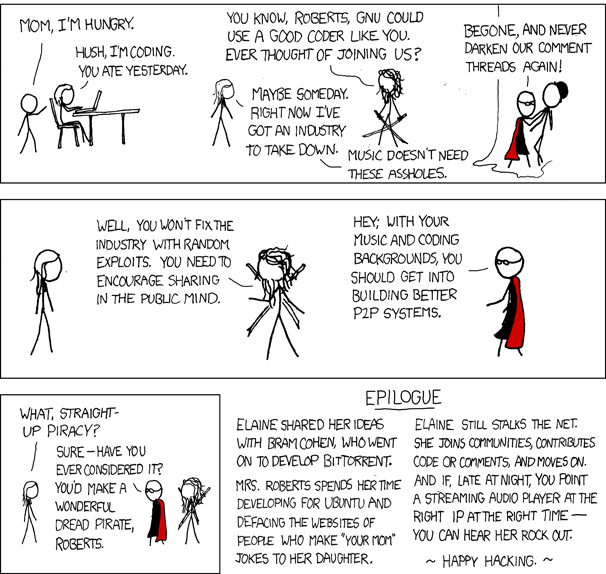
\includegraphics[keepaspectratio,width=0.9\textwidth]{elements/images/1337_part_5_2.png}\\
  \textline[t]{\tiny{\textit{s.\pageref{13375a} $\leftarrow$ föreg.}}}{\tiny{BY-NC 2.5 xkcd.com}}{}\par
\end{center}\par
\vfill
\null
\chapterpageimage{Register}{Register}{elements/register.jpg}
\cfoot{}
\newgeometry{top=1cm,bottom=1.2cm,left=1cm,right=1cm,footskip=0pt,headsep=0.2cm,footskip=0.5cm}
\small
\printindex
\newpage
\ohead{}
\newpage
\null
\newpage
\null
\newpage
\null
\newpage
\null
\newpage
\null
\end{document}
